\documentclass[openany]{report}
%\documentclass[a4paper]{book}
\usepackage[utf8]{inputenc}
\usepackage[T1]{fontenc}
\usepackage[english]{babel}
\usepackage[table,dvipsnames]{xcolor}
\usepackage{xspace}
\usepackage[title]{appendix}
\usepackage{wrapfig}
\usepackage{graphicx}
\usepackage{subcaption}
\usepackage{csquotes}
\usepackage{longtable,array,booktabs,makecell}
\usepackage{booktabs}
\usepackage{quotes}
\usepackage{awesomebox}
\usepackage{ltablex}
\usepackage{tablefootnote}
\usepackage[pdfpagelabels]{hyperref}
\usepackage{lscape}


\title{The Mega Man X Compedium}

\newcommand{\x}{\textit{X1}\xspace}
\newcommand{\mhx}{\textit{MHX}\xspace}
\newcommand{\PtIIWarning}{Part \ref{assumptions} preface}
\newcommand{\portraitsize}{5cm}
\hypersetup{
	colorlinks=true,
	linkcolor=blue,
	urlcolor=cyan,
	citecolor=red,
	pdftitle={The Mega Man X Compendium}
}
\newcommand{\enemSpecs}[3]{\begin{itemize}
			\item \textbf{HP}: #1
			\item \textbf{Damages}: #2
			\item \textbf{Description}: #3
		\end{itemize}}
	
\newcommand{\tabline}{\hskip-0.5pt\vrule width 1pt\hspace{\labelsep}}
\newcommand{\tabdot}{\makebox[0pt]{\textbullet}\tabline}

\newcommand{\timepoint}[1]{\tabdot & #1 \\}
\newcommand{\timemoment}[1]{\tabline & $\cdot$ #1 \\}

\begin{document}
\pagenumbering{Alph}
\begin{titlepage}
	\maketitle
	\thispagestyle{empty}
\end{titlepage}
\pagenumbering{arabic}

\tableofcontents

\part{Games}
	\section*{Preface}
	This document aims to serve as a comprehensive compendium of all available knowledge on the Mega Man X games, encompassing both the main plot/lore and game mechanics. It will also include trivia, fun facts, and even glitches/bugs. Each game in the series will be covered with information regarding its story, characters (albeit in a superficial manner), weapons, and game mechanics. Additionally, a thorough analysis of each stage, including its secrets and boss (with both story-related and game-related details), will be provided.
	
	Following the analysis of the games, a more accurate and complete description of each character will be presented. This will be achieved by combining information from various sources, including in-game content and other official materials.
	
	It is important to note that this document is designed to be accessible and understandable to everyone, catering to experienced players and newcomers alike. It accommodates those seeking to dive deeper into the series' lore and those who wish to uncover tricks and secrets in each game.
	
	Furthermore, this document is open for editing by anyone. It welcomes suggestions for additions if something is missing or modifications if any errors are found.
	
	Finally, it is essential to clarify that this document does not intend to be a guide for new players or speedrunners. While it will offer some tips for both categories, readers should not consider the content here as a definitive guide of any sort.
	
	\section*{How to read this document}
	While perusing the document, readers will come across words or numbers highlighted in different colors. These serve as links, connecting various sections and chapters within the document, facilitating seamless navigation for the reader. The color codes and their corresponding functions are as follows:
	\begin{itemize}
		
	\item \textcolor{blue}{Blue text}: These are links to other sections of the document that provide a more in-depth analysis of the referenced topics.
	
	\item \textcolor{red}{Red numbers}: These indicate bibliographic references within the text and are presented with an entry number in square brackets. Clicking on these numbers will direct the reader to the corresponding entry in the bibliography section.
	
	\item \textcolor{cyan}{Cyan words}: These are URLs that lead to web pages, typically serving as sources of bibliographic material.
	\end{itemize}
	
	Furthermore, recognizing that certain concepts may require visual demonstration, a video folder accompanies this document. Inside, readers will find short video demonstrations complementing the explanations provided in the text
	
	
\chapter{Mega Man X}
\label{cha:X1}
%	%MEGA MAN X.TEX

\textit{Mega Man X} is born as a spin-off game of the classic Mega Man franchise for the Super Famicon/SNES consoles (later also for PC)  between the 1993 and the 1995~\cite{wiki:MMX}. The game takes place one hundred years after the main franchise timeline, in a world where humans and special robots capable of having feelings co-exists and where X, one of those robots, fights the evil Sigma which aims to eliminate humans on order to create a world only for robots.

\begin{figure}[htp]
	\centering
	\begin{subfigure}{0.4\linewidth}
		\centering
		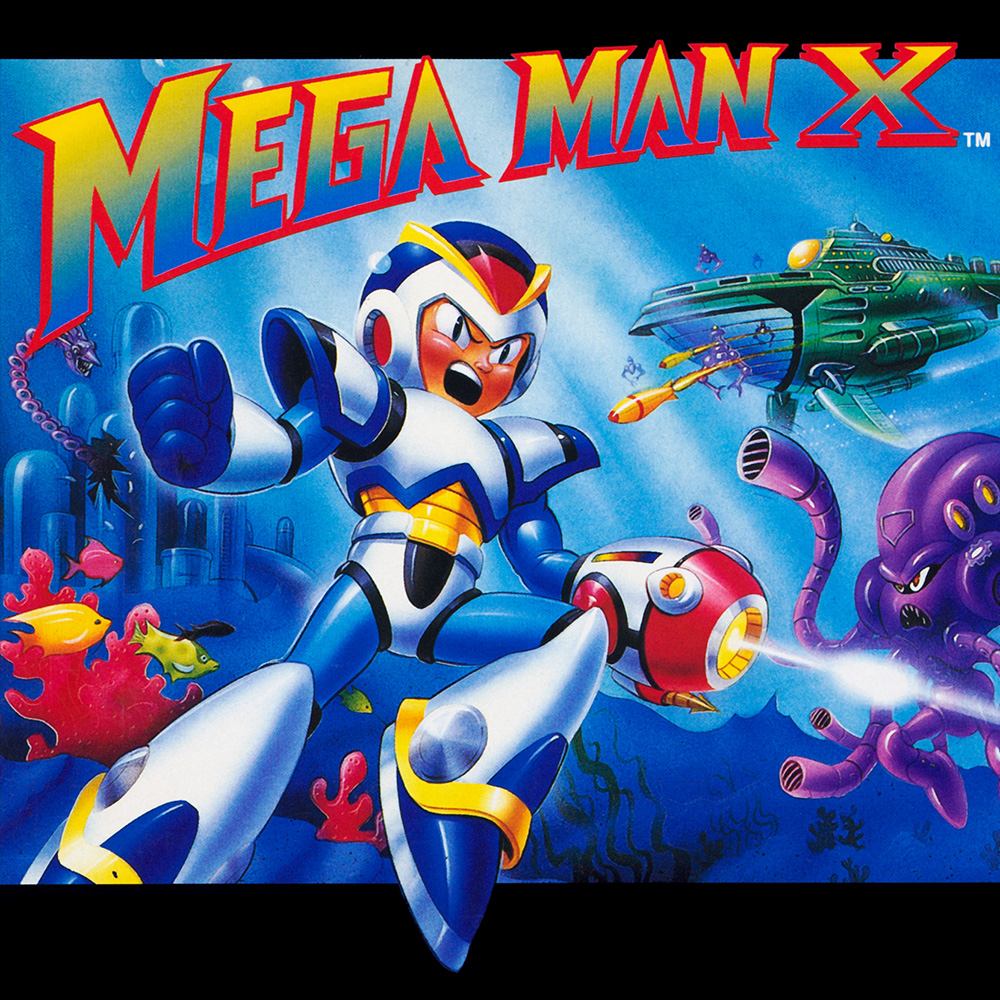
\includegraphics[width=\linewidth]{figures/X1/mmx_cover.jpeg}
	\end{subfigure}
	\begin{subfigure}{0.4\linewidth}
		\centering
		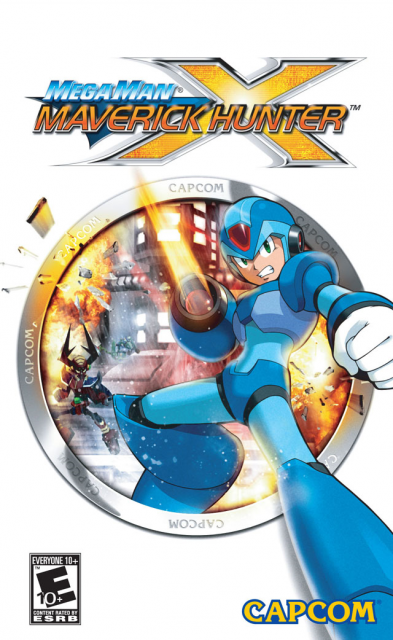
\includegraphics[width=\linewidth]{figures/X1/mmxmh.png}
	\end{subfigure}
\end{figure}

In the year 2005 a remake of the game was done for PlayStation Portable, upgraded to a 3D graphic close to the precedent title, Mega Man X8. This game (named \textit{Maverick Hunter X }or \mhx in short) had the purpose to re-tell the first game's story with some minor changes such as X relationship with Mavericks and Sigma, which weren't present in the original game. Changes also effected level design, such as Light's capsule positions or Sigma stages, completely different from original ones.



\section[Main plot]{Main plot (X)}
In the year 21XX humans live peacefully with new kind of robots: reploids. Reploids are particular type of robots with the ability to take autonomous decisions as well as having feelings and sentiments~\cite{Xcoll1:Manual_X1}. However sometimes  a reploid's electric brain can undergo  malfunctioning making him act dangerously for nearby humans and others reploids . When this happen the reploid is labeled as ``Maverick'' and has to be stopped, in order to be repaired or disposed, by a special organization created with the exact purpose to stop mavericks: the Maverick Haunters. Leader of the Maverick Haunters is Sigma, one of the most advanced reploid of the time. 

The situation takes a turn when Sigma himself go maverick, declaring war against humanity and recruiting in its rank other maverick haunters, both willing to follow him or threatened by Sigma himself. In order to stop the war X, the main protagonist of the story, decides to joining the fight alongside Zero, a close friend of him, on the battlefield, an highway currently under attack. There he is however stopped by Vile, an ex-haunter released by Sigma from prison, in his ride armor. Only the intervention of Zero himself, which force Vile to flee, allow X to escape safely.
\begin{figure}[htp]
	\centering
	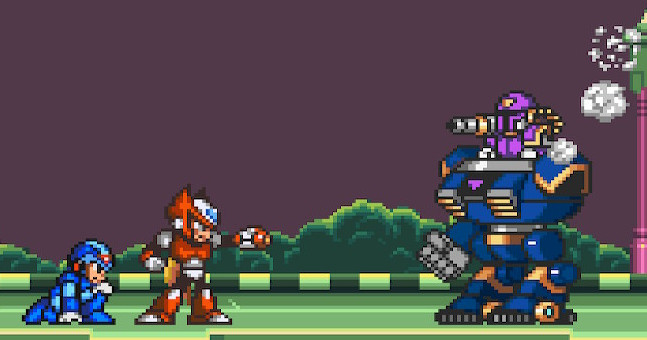
\includegraphics[width=0.5\linewidth]{figures/X1/Highway_end.jpg}
	\caption{Zero saving X from Vile.}
\end{figure}

The two then decide to split: while Zero goes to locate the enemy fortress, X has to deal with the threat of Sigma's mavericks. As X defeats all the eight mavericks, acquiring in the process new power-ups and strength, he joins Zero who in the meanwhile has located the Sigma fortress flying over the sea. At the entrance however they are immediately confronted with Vile and his ride armor, which first manages to capture Zero (that challenged him in a one-versus-one fight) and subsequently X too. As Vile laughs at his victory, Zero manages to escape from his cage, latches on the ride armor and detonates himself, destroying it but leaving Vile untouched. Seeing his friend's action give X new energy, allowing him to break free too and face Vile, now vulnerable, defeating him in the process. Before going on however X listens to Zero's ultimate words~\cite{wiki:MMX_script}. Zero informs X that his auto-repair system cannot handle all damages taken and that X has a power even greater than his own, which makes him capable of face Sigma (eventually Zero also gives X his own Z-buster if he didn't manage to get his own buster upgrade).
\begin{figure}[htp]
	\centering
	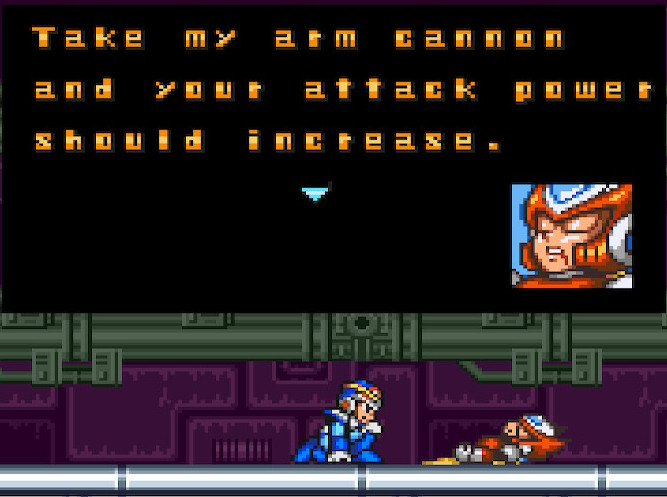
\includegraphics[width=0.5\linewidth]{figures/X1/Zero_cannon.jpg}
	\caption{Zero, near death, giving X his arm cannon.}
\end{figure}
After that, Zero dies and X proceeds infiltrating Sigma's fortress and his dangers, including re-facing all the previously-defeated mavericks. At the end X arrives at Sigma's place where Sigma is waiting. At first Sigma acts with arrogance, looking surprised that X has managed to reach him with his only forces and claiming he could destroy him without effort. However he decides to leave the pleasure to his pet Velguarder, as he leaves the scene to assist at the fight. After X successfully manages to destroy Velguarder, Sigma changes his mind a little, understanding why Zero placed his trust in X and claiming X could have been an haunter as strong as he was. After that he proceeds to confront X on his own, but gets defeat and his body destroyed so that only his head remaining, which subsequently proceed to merge with a giant wolf-based mechaniloid in the room, giving Sigma a new body to fight X. However X succeeds in destroying the new body as well, effectively getting rid of Sigma for good. As Sigma blames X for destroying his dream of a world only for reploids, Sigma himself and the fortress start to explode, forcing X to teleport to the outside. In the end X ponders about the destruction he helped to generate, on the sacrifices made for the victory, and questioning if choosing to fight was the right choice, meditating if another option was possible. As the flying fortress sinks in the ocean, X realizes that he will have to fight more battles before having the answers he needs. 
After the game's credits, it is however revealed that the next battle will not take long before occurring, since a message form Sigma is played, where the maverick states that his spirit is still intact and waiting for a new body to be built to face X again.
\begin{figure}[htp]
	\centering
	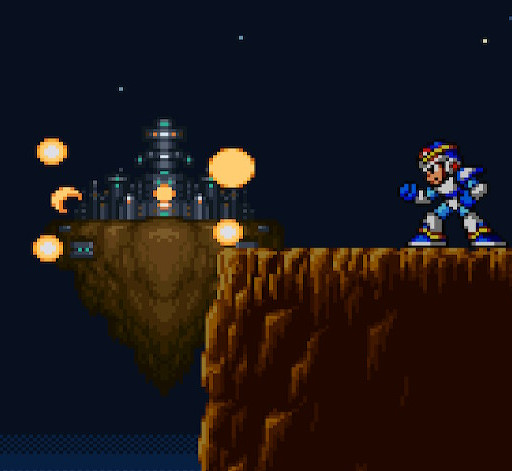
\includegraphics[width=0.45\linewidth]{figures/X1/Ending.jpg}
	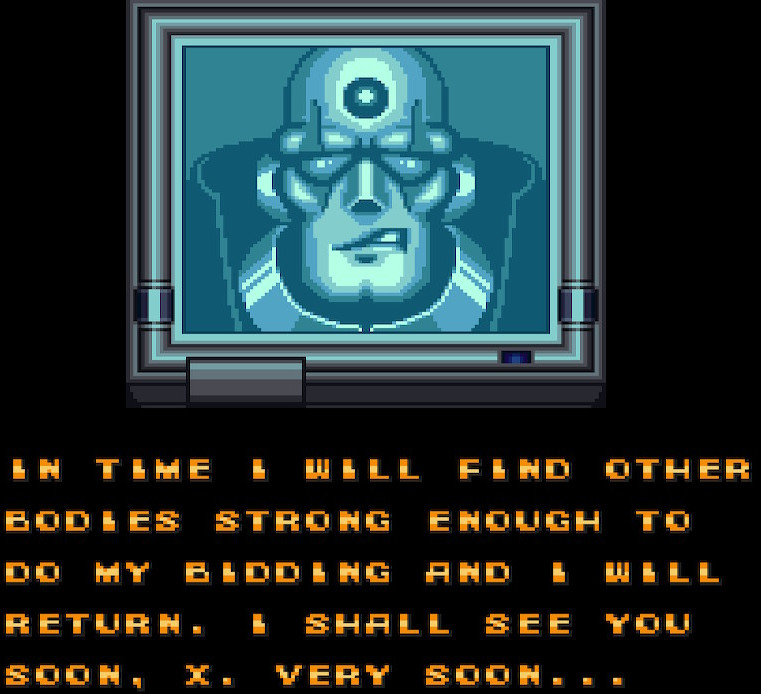
\includegraphics[width=0.45\linewidth]{figures/X1/sigma_message.jpg}
	\caption{Sigma's fortress sinking in the ocean and Sigma's final message to X.}
\end{figure}

\section{Main Plot (\mhx)}
While being for the major part similar to the original plot, \textit{Maverick Haunter X} takes some divergence regarding characters relationship as well as X's background~\cite{wiki:MM_MHX}. One of the main divergence point regard X's story prior to the war's beginning. Next is a summary of \textit{Maverick Haunter X} differences respect \x.
\begin{itemize}
\item An in-depth background of the war is given, via the ``Day of $\Sigma$"" OVA, explaining how Sigma started his revolution. Here X's background is also changed, now already being a Maverick Haunter (in contrast with the original, where no information are available) serving in the 17th Elite Unit alongside Zero and commanded by Sigma himself. X's haunter rank is B (in contrast to Zero's SA rank) due to his kindness and pacifist spirit making him prefer dialogue over fighting, traits which most mistake for weakness. The only ones suspecting of his true potential are again Zero and Sigma. 

\item Another character with an expanded background is Vile. Here he aims to destroy both X and Sigma, to create his own world, hence following Sigma plans only due the fact some objectives they have match.

\item A main difference between games regards the final portion of the story~\cite{wiki:MM_MHX_script} and in particular final level's layout. In fact, while in the original X and Zero immediately face Vile as they enter Sigma fortress, here X first travel through the fortress, facing previous bosses brought back to life, and only at end he meets with Zero and is stopped by Vile. As the main story, however, Vile captures both of them, resulting in Zero sacrificing himself and X destroying him. 
\item Finally, even Sigma has a different attitude regarding X due already suspecting X's great potential. In fact he first tests X by making him fight Velguarder (in contrast with the original game, where Sigma use Velguarder thinking to be sufficient to defeat X) and then challenges X himself, ending in the same way as the original story.	
\end{itemize}

\section{Main Characters}
\subsection{X}
\begin{figure}[htp]
	\centering
	
\includegraphics[width=0.3\linewidth]{figures/X1/X_X1.png}
	\caption{X}
\end{figure}
X (see chap.~\ref{char:X} for full information) is the first type of a new kind of sentient robot capable of having feeling and take decision of his own, developed by Dr. Thomas Light in the year 20XX. Being provided with great power, Dr. Light needed to ensure X's integrity by running a series of test which would have required thirty years to be completed. Unlikely, Dr. Light lifespan didn't allow himself to live longer to complete all tests, so he sealed X in a capsule capable of running tests in autonomy.

In the year 21XX X's capsule is found by Dr. Cain (chap. \ref{char:Cain}) during an archaeological expedition~\cite{X:Manual},~\cite{wiki:Cain_journal}. Dr. Cain awakes X and, using Light's designs and X's help, develops a new kind of robot  which he names ``Reploids'' which quickly integrate in the society due their great contribute in doing hard tasks. X however remains questioning about his place in the world and the future Dr. Light wanted for him. Despite this, when the evil Sigma starts his war against human kind, X is forced to step up and fight in order to restore peace alongside his friend Zero. 

What told until now refers to the original role of X in the \x game. Nevertheless, as stated before, \textit{Maverick Haunter X} re-write X's story by providing a new background for events prior to Sigma's revolt. In this continuity Dr. light seals X away not for testing his integrity, but rather believing the world not to be ready for X's technology and potential. Here Light is firmly convinced that X has a good spirit and that he will use his power to achieve peace~\cite{wiki:MM_MHX_X}. Moreover after his awakening X joins the Maverick Haunters (which do not happen in the original story), serving in the 17th Elite Unit, alongside Zero and under the direct command of Sigma. Despite having great potential, however, X's haunter rank is only B (in contrast with the SA rank of Zero) due is what seems to be his lack of decision during battle. In reality this is caused by his pacifist nature, making him reluctant to fight and preventing him to use his real power~\cite{Xcoll1:Manual_X1}. Nevertheless, when the evil Sigma starts his war against human kind, X is forced to step up and fight in order to restore peace together with Zero.

\subsection{Zero}
\begin{figure}[htp]
	\centering
	
\includegraphics[width=0.3\linewidth]{figures/X1/Zero_X1.png}
	\caption{Zero}
\end{figure}
Fighting alongside X against Sigma is Zero (see chapter~\ref{char:Zero}). In the original \x game, very few information are give regarding Zero, except being a friend of X and the new leader of the Maverick Haunters~\cite{X:Manual}, having the highest rank above all haunters which didn't side with Sigma. 
Different is the situation in the \mhx game, where Zero's relationship with X is explained better, the former being a close friend and a mentor to X in the 17th Elite Unit, having an SA haunter rank and working under Sigma. Here it is also stated how Zero repel evil with all his strength, fighting merciless against Maverick, Sigma included~\cite{Xcoll1:Manual_X1}.  

In any case, Zero story is the same for both games. He first appears at the end of the highway saving X from Vile's grasp, and asking X to take care of Sigma forces while he locates the enemy hideout. Next he's seen at the entrance of Sigma fortress where he suggests to split up, offering to act as decoy to let X sneak inside. Lastly Zero is seen for the last time at the final battle with Vile, where he sacrifices himself to destroy Vile's armor and allow X to defeat him. Finally with his last words he ask X to go and take down Sigma, eventually giving X his own Z-buster, in case X hasn't upgraded it yet.

\section{Game Mechanics}
\textit{Mega Man X}'s gameplay stays faithful to its original series by being a 2D hybrid between a run'n'gun game and a platformer, where the main protagonist (X in this case) has to clear different stages in order to unlock the final area of the game. Each stage has its own theme, contains a certain number of items to collect (depending on the stage it could be one ore more) which may require other power-ups to be collected first in order to be obtained (typically bosses weapons). Finally at the end of the stage a boss waits, which has to be defeat in order to clear the stage and which will give X a new weapon based on one of his attacks. As the original series all main stages can be accessed in any order and all bosses presents have a ``weak point'' corresponding to a weapon obtained from defeating one another boss first. The ``weak point'' typically consists in a weapon dealing more damage to the boss, but sometimes others effects can occur, such has stunning him or preventing the boss to do certain actions.

\x introduces however some new mechanics which will later define the series~\cite{wiki:X1_features}:
\begin{itemize}
	\item Dash: X, via the boot parts, can dash and move faster, as well as jump higher via a dash-jump. It can be considered an evolution of the sliding mechanism, as it is tie to a specific button instead of a combination of two buttons.
	\item Wall-jumping: X can jump onto wall in order to climb them or can slide down to descend slowly. He can also dash-jump off to a wall to cover a greater distance.
	\item Armor parts (sec. \ref{X1:Armor}): By finding Light's capsules (four in total) X can be upgraded unlocking new powers which can help the player during the game.
	\item Sub-Weapon charging (sec.~\ref{X1:sub_weapon}): via the buster upgrade, X can not only charge his main X-buster, as in the main series, but he can also charge his other sub-weapon to increase damage dealt or change their functionalities.
	\item Heart tanks: beside classical Sub-tank X, eight heart tank are also scattered in various stages (one per each). By picking them up X's energy grows by two, starting from 16 up to a maximum of 32~\cite{stratwiki:Heart_tank}.
	\item Stage interactions: although a very limited feature, by clearing certain stages, other ones will be effected and change in some portions.
\end{itemize}

\section{Weapons}\label{X1:sub_weapon}
Here is a list of all sub-weapons available in\textit{ Mega Man X}/ \textit{Mega Man Maverick Haunter X} (\cite{MHX:manual}, \cite{wiki:X_weapons}):

\subsection{
\includegraphics[scale=0.2]{figures/X1/weapons/Homig_T.jpg} Homing Torpedo}\label{Homing_torpedo}
When equipping this sub-weapon X gains the ability to fire up to two (three in \mhx)~\cite{wiki:Homing_torpedo} torpedoes capable of tracking enemies. As they pick up speed, they home in on the closest enemy and pursue it. When charged X will release a fan of four (six in \mhx) fish-shaped missiles with greater speed and attack power which home better to enemies. This weapon is obtained after defeating Launch Octopus (sec.~\ref{boss:Launch_octopus}).
\begin{figure}[htp]
	\centering
	\begin{subfigure}{0.39\linewidth}
		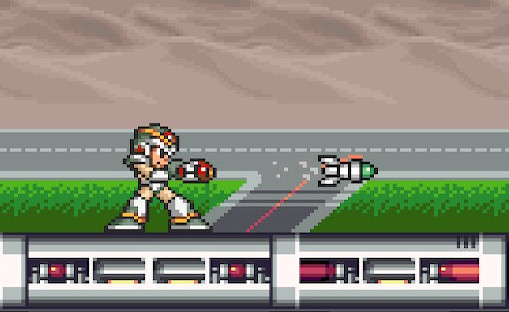
\includegraphics[width=\linewidth]{figures/X1/weapons/Homing_torpedo_1.jpg}	
	\end{subfigure}
		\begin{subfigure}{0.3\linewidth}
		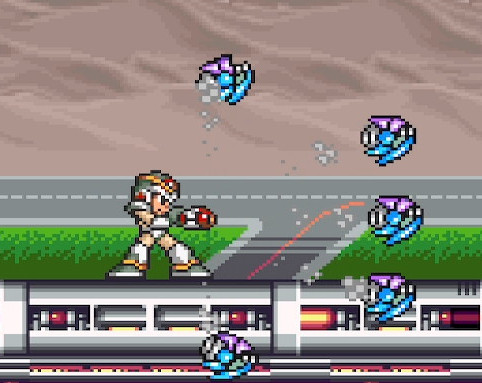
\includegraphics[width=\linewidth]{figures/X1/weapons/Homing_torpedo_2.jpg}	
	\end{subfigure}
	\caption{Homing Torpedo sub-weapon's regular and charged attack.}
\end{figure}

\subsection{
\includegraphics[scale=0.2]{figures/X1/weapons/C_sting.jpg} Chameleon Sting}\label{Chameleon_sting}
The Chameleon Sting, obtained after beating Sting Chameleon (sec.~\ref{boss:Sting_chameleon}), emits a single straightforward laser which than splits into three directions: forward, up-forward, down-forward. In \mhx it instead directly emits three lasers, which can be angled diagonal-up and diagonal-down and are slightly faster. In both games the charged version makes X flash in various colors of the rainbow making him invincible to any damage (besides insta-kill hazards like pits) for a short amount of time. In the original game X cannot switch to any weapon while the invincibility is active, meanwhile in the remake is free to fire both with the current one and any other weapon~\cite{wiki:Chameleon_sting}.
\begin{figure}[htp]
	\centering
	\begin{subfigure}{0.35\linewidth}
		
\includegraphics[width=\linewidth]{figures/X1/weapons/Chameleon_sting.jpg}
	\end{subfigure}
	\caption{Chameleon Sting sub-weapon}
\end{figure}

\subsection{
\includegraphics[scale=0.2]{figures/X1/weapons/Rolling_S.jpg} Rolling Shield}\label{Rolling_shield}
After beating Armored Armadillo (sec.~\ref{boss:Armored_Armadillo}), X will gain the Rolling Shield. By using it X spins energy at high speeds within the X-Buster and launches it as an energy shot that rolls along the ground. The generated projectile is about the same size as X (half in \mhx) and will roll following the ground until making contact with an enemy or disappear after a while. Only in \mhx the shield will absorb any projectile directed toward it, as well as dispose Mets even while hiding~\cite{wiki:Rolling_shield}. Upon contact whit a wall, the shield will ricochet once and disappear up hitting a wall again. When charged X will surround himself with an energy field which eliminates any enemy with less than three hit points that makes contact, but will disappear upon hitting enemies with more than that life value. In the original game while the charged shield is active X cannot shoot nor change weapon while in game, requiring the player to change weapon from the pause menu and thus making the shield disappear.
\begin{figure}[htp]
	\centering
	\begin{subfigure}{0.35\linewidth}
		
\includegraphics[width=\linewidth]{figures/X1/weapons/Rolling_shield_1.jpg}	
	\end{subfigure}
	\begin{subfigure}{0.3\linewidth}
		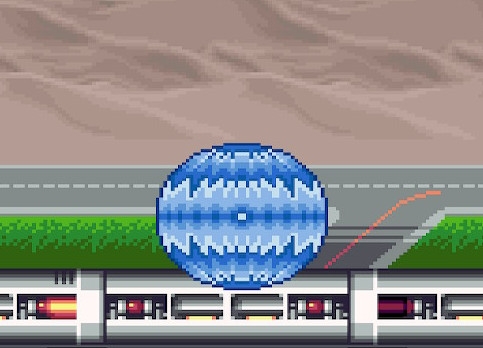
\includegraphics[width=\linewidth]{figures/X1/weapons/Rolling_shield_2.jpg}	
	\end{subfigure}
	\caption{Rolling Shield sub-weapon's regular and charged attack.}
\end{figure}

\subsection{
\includegraphics[scale=0.2]{figures/X1/weapons/F_wave.jpg} Fire Wave}\label{Fire_wave}
Fire Wave converts the X-buster into a powerful flamethrower, which deals continuous damage to enemies but that cannot be used underwater. Upon pressing the fire button X will start shooting fire from his X buster at a continuous rate draining energy in the process. Once charged X will fire a fireball which creates a pillar of fire upon hitting the ground and that moves forward for a while. However in order to charge the weapon X must keep firing, draining energy in the process. If used underwater the weapon won't work, only producing smoke (but still draining energy)  This weapon is obtained once Flame Mammoth is defeated (sec.~\ref{boss:Flame_mammoth}). 
\begin{figure}[htp]
	\centering
	\begin{subfigure}{0.35\linewidth}
		\centering
		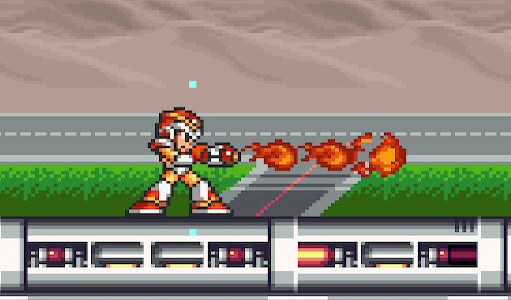
\includegraphics[width=\linewidth]{figures/X1/weapons/Fire_wave_1.jpg}
	\end{subfigure}
	\begin{subfigure}{0.35\linewidth}
		\centering
		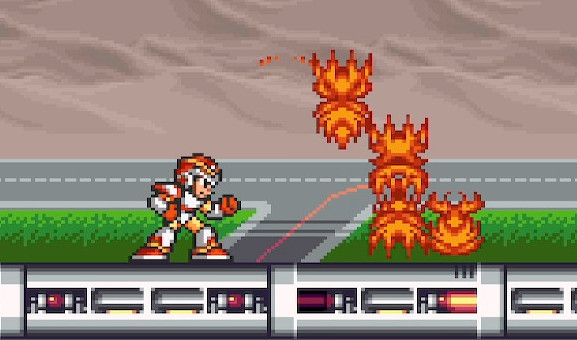
\includegraphics[width=\linewidth]{figures/X1/weapons/Fire_wave_3.jpg}
	\end{subfigure}
\end{figure}
\begin{figure}[htp]
	\ContinuedFloat
	\centering
	\begin{subfigure}{0.34\linewidth}
		\centering
		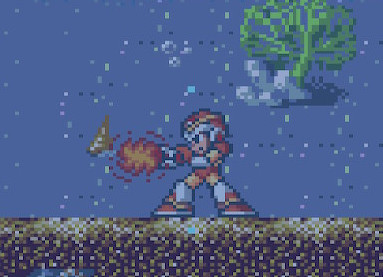
\includegraphics[width=\linewidth]{figures/X1/weapons/Fire_wave_2.jpg}
	\end{subfigure}
	\begin{subfigure}{0.36\linewidth}
		\centering
		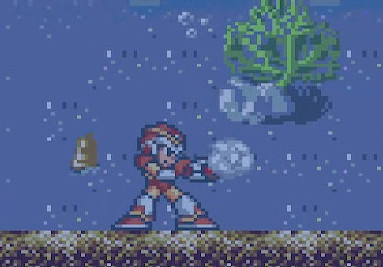
\includegraphics[width=\linewidth]{figures/X1/weapons/Fire_wave_4.jpg}
	\end{subfigure}
	\caption{Fire Wave sub-weapon's regular and charged attack both outside and inside water.}
\end{figure}


\subsection{
\includegraphics[scale=0.2]{figures/X1/weapons/Storm_T.jpg} Storm Tornado}\label{Storm_tornado}
The Storm Tornado turns the X-buster into a high-power fan that blasts opponents with hard-hitting wind, capable of destroying enemies that stand in its path. It shoots an horizontal tornado which stays on the screen for a short amount of time, and then starts moving in the direction X was facing when shot. Due to his length it can hit enemies multiple times, being an effective way to dispose most of them, especially bigger ones.  The \mhx version has its length halved, which allows to shoot it at a faster rate. When charged the Storm Tornado will create a large vortex covering all the screen in high, which surrounds X in the original game while explodes instead from a shot projectile once it hits a solid surface in the remake~\cite{wiki:Storm_tornado}. It is obtained by defeating Storm Eagle (sec.~\ref{boss:Storm_Eagle}).
\begin{figure}[htp]
	\centering
	\begin{subfigure}{0.35\linewidth}
		
\includegraphics[width=\linewidth]{figures/X1/weapons/Storm_tornado_1.jpg}
	\end{subfigure}
	\begin{subfigure}{0.25\linewidth}
		
\includegraphics[width=\linewidth]{figures/X1/weapons/Storm_tornado_2.jpg}
	\end{subfigure}
	\caption{Storm Tornado sub-weapon's regular and charged attack.}
\end{figure}

\subsection{
\includegraphics[scale=0.2]{figures/X1/weapons/E_Spark.jpg} Electric Spark}\label{Electric_spark}
Electric spark creates high-pressure voltage within the X-Buster and fires it, for a maximum of three shots at time. If the electric spark hits an hard surface, it splits in half, starting to travel up and down along the surface. The charged version of this weapon differs between the original game and his remake. In X1 upon charged X will release two electric columns in front and behind him and which will move in their respective directions, while in \mhx X will generate electricity in all directions from his body, covering the entire screen. This weapon is acquired upon defeating Spark Mandrill (sec.~\ref{boss:Spark_mandrill}).
\begin{figure}[htp]
	\centering
	\begin{subfigure}{0.35\linewidth}
		
\includegraphics[width=\linewidth]{figures/X1/weapons/Electric_spark_1.jpg}
	\end{subfigure}
	\begin{subfigure}{0.25\linewidth}
		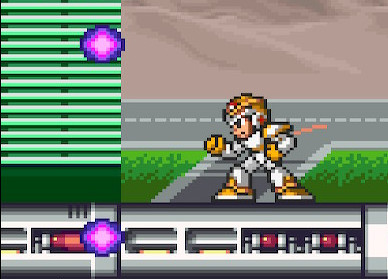
\includegraphics[width=\linewidth]{figures/X1/weapons/Electric_spark_2.jpg}
	\end{subfigure}
	\begin{subfigure}{0.3\linewidth}
		
\includegraphics[width=\linewidth]{figures/X1/weapons/Electric_spark_3.jpg}
	\end{subfigure}
	\caption{Electric Spark sub-weapon's regular (normal and split) and charged attack.}
\end{figure}

\subsection{
\includegraphics[scale=0.2]{figures/X1/weapons/B_cutter.jpg} Boomerang Cutter}\label{Boomerang_cutter}
The Boomerang Cutter is the weapon obtained by defeating Boomer Kuwanger (sec.\ref{boss:Boomer_Kuwanger}). It fires up to three~\cite{wiki:Boomerang_cutter} sharp boomerangs made from a special metal whose trajectory depends on the position X was when he fired them: they will arc upwards if X was standing on the ground, while they will arc downwards if X was in the air. If a boomerang does not hit an enemy, it returns to its owner, and if it passes an item on its way back, it picks up the item and delivers it to its own owner (even bringing dropped life/weapon energy from enemies). If a boomerang successfully return to X without hitting an enemy, it will replenish the energy used to create it. Upon charged X will release four bigger boomerang spiraling out of him diagonally. In \mhx this has been changed with four boomerang of doubled size which will move back and forward in straight line a few times. 

This weapons has, finally, a special perk. Both Flame Mammoth and Launch Octopus, in fact, while not being directly weak to Boomerang Cutter can be heavily damaged when hit with this weapon, the former loosing his trunk and the latter his tentacles, resulting in both being unable to perform certain attacks anymore.
\begin{figure}[htp]
	\centering
	\begin{subfigure}{0.3\linewidth}
		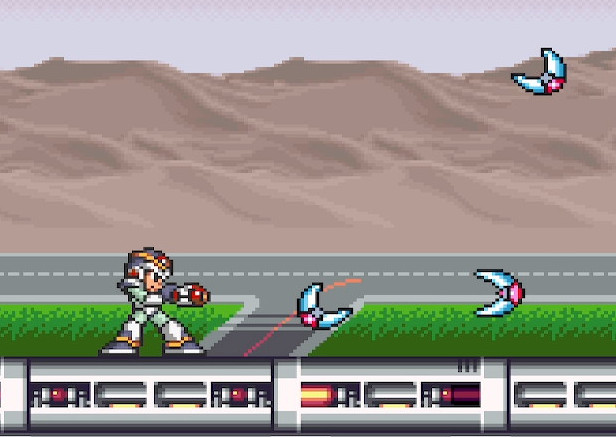
\includegraphics[width=\linewidth]{figures/X1/weapons/Boomerang_1.jpg}
	\end{subfigure}
	\begin{subfigure}{0.3\linewidth}
		
\includegraphics[width=\linewidth]{figures/X1/weapons/Boomerang_2.jpg}
	\end{subfigure}
	\caption{Boomerang Cutter sub-weapon's regular and charged attack.}
\end{figure}

\subsection{
\includegraphics[scale=0.2]{figures/X1/weapons/S_ice.jpg} Shotgun Ice}\label{Shotgun_ice}
Shotgun Ice is the weapon obtained by X after defeating Chill Penguin (sec.\ref{boss:Chill_Penguin}). It absorbs moisture in the air and fires it in crystallized form. If it hits an enemy or a hard surface, it breaks into 5 pieces which ricochet backward and get destroyed if hit another wall or enemy. When charged the weapon creates a Chill Penguin-shaped ice platform (only in \x, while in \mhx is only a sharp sled of ice) in similarly to how the boss creates his ice sculpture. X can stand on the platform which will start moving forward shortly after being created. If X creates the platform and then places himself in the same spot where the platform is creating (due the fact that the creation in not immediate) the platform will slightly push X left or right depending of its position, enabling some glitches such as wall clipping( sec.~\ref{X1:misc}, only in \x).
\begin{figure}[htp]
	\centering
	\begin{subfigure}{0.3\linewidth}
		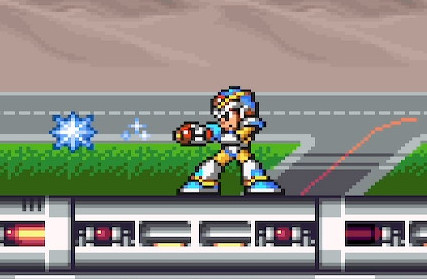
\includegraphics[width=\linewidth]{figures/X1/weapons/Shotgun_ice_1.jpg}
	\end{subfigure}
	\begin{subfigure}{0.31\linewidth}
	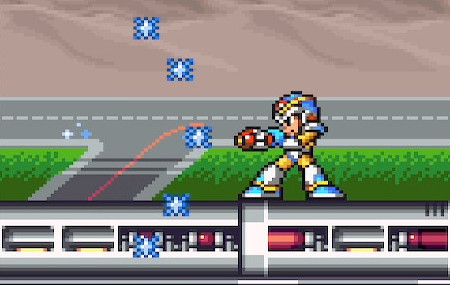
\includegraphics[width=\linewidth]{figures/X1/weapons/Shotgun_ice_2.jpg}
	\end{subfigure}
	\begin{subfigure}{0.29\linewidth}
		
\includegraphics[width=\linewidth]{figures/X1/weapons/Shotgun_ice_3.jpg}
	\end{subfigure}
	\caption{Shotgun Ice sub-weapon's regular (normal and deflected shots) and charged attack.}
\end{figure}


\section{First Armor}\label{X1:Armor}

While exploring stages X can run into one of the four capsules hidden by Dr.~Light. When X makes contact with the capsule, it will open revealing Dr.~Light's hologram which will talk to X and give him one of the armor parts~\cite{wiki:First_armor}, explaining in the process how it works.
\begin{figure}[htp]
	\centering
	
\includegraphics[width=0.2\linewidth]{figures/X1/First_armor.png}
	\caption{First armor X.}
\end{figure}

The First Armor is composed by the following parts:
\begin{itemize}
	\item Foot Parts:	Namely ``Emergency Acceleration System''~\cite{X:Manual} allow X to dash forward, as well as to perform dash-jumps and wall dash-jumps, also reducing his hitbox's height a little while dashing.
	 \begin{figure}[htp]
		\centering
		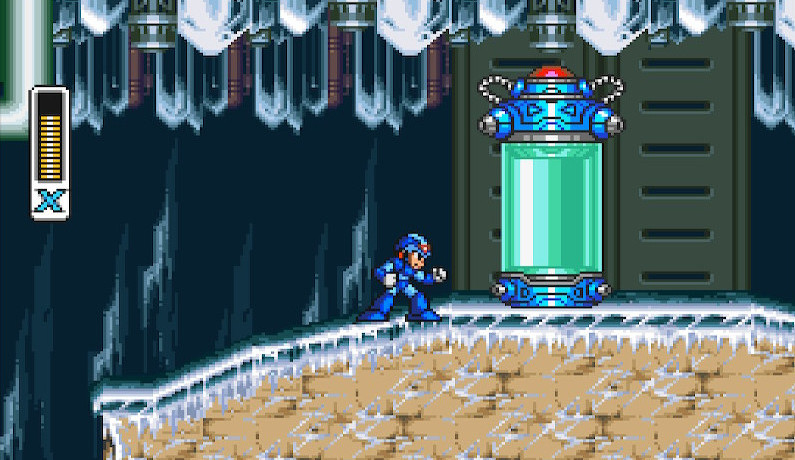
\includegraphics[width=0.4\textwidth]{figures/X1/Chill_penguin/Armor_foot.jpg}
		\caption{Foot Part capsule location}
	\end{figure}
	Moreover X can destroy specifics blocks by wall-jumping onto them. The capsule containing the foot parts reside right in the middle of the Snow Mountain Stage, being mandatory to take. In \mhx the capsule is instead at the beginning of the Factory Stage.
	
	
	\item Body Parts: When equipped, X will have all incoming damage reduced by 50\%. It is found in the Forest stage after climbing the wall right before the cave. After defeating RT-55J the capsule will emerge from the ground. Meanwhile \textit{Maverick Haunter X} has moved it in Storm Eagle Stage, requiring the head part to access it.
	\begin{figure}[htp]
		\centering
		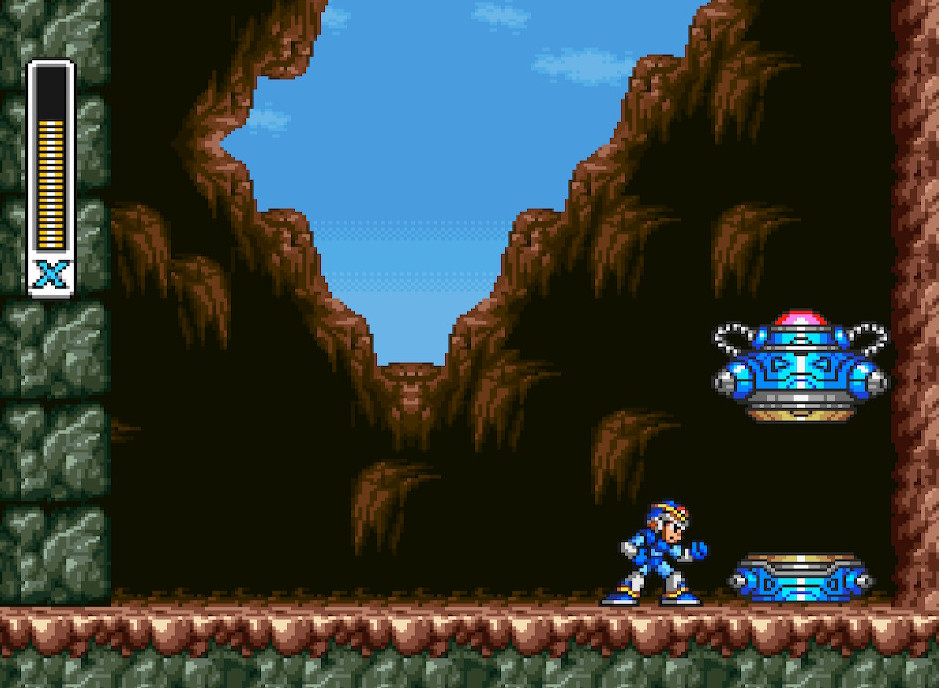
\includegraphics[width=0.4\textwidth]{figures/X1/Sting_chameleon/Sting_armor_capsule.jpg}
		\caption{Body Part capsule location}
	\end{figure}
	
	\item Arm Parts: Allow the X-Buster to be charged up to a third level, and to charge up special weapons. Originally Dr. Light thought this upgrade to be included in the basic X-Buster~\cite{X:Manual}, but he sealed away X when the upgrade was not ready yet, forcing him to turn it into a modification to give to X only later.
	\begin{figure}[htp]
	\centering
	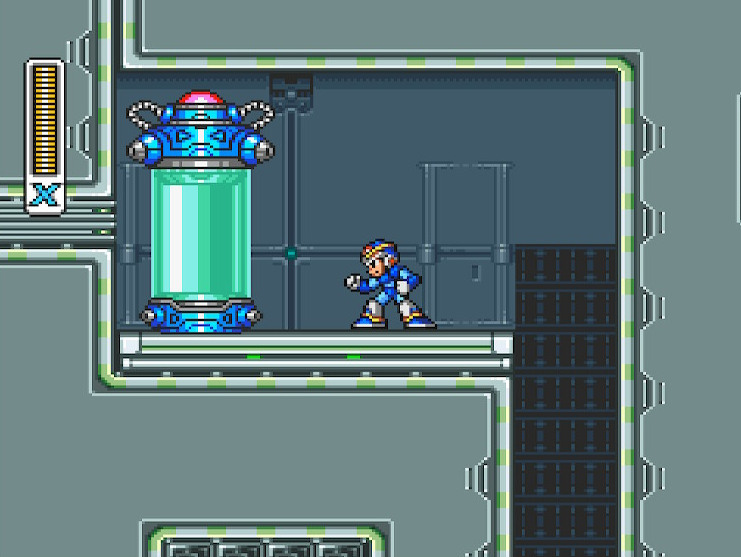
\includegraphics[width=0.4\textwidth]{figures/X1/Flame_mammoth/Flame_armor_2.jpg}
	\caption{Arm Parts capsule location}
	\end{figure}

	Despite the capsule itself not being mandatory, the game will in any case give the player the buster upgrade in form of the Z-Buster if the player arrives at facing Vile without having found the capsule first. While in \x there are no differences between the Arm Parts and the Z-Buster, in \mhx the former allow to shoot the Spiral Crush Buster, which has the same power of the second-level charged shot but is larger and hit multiple times, while the latter deals more damage against bosses that the previous alternative. In \textit{Meg Man X} the capsule reside in the Factory stage, requiring a precise dash-jump and the Head Parts to break some blocks in the ceiling, while in the remake it is in the same place the Body Parts was in the original game.
	\begin{figure}[htp]
		\centering
		
\includegraphics[width=0.5\textwidth]{figures/X1/weapons/Buster_4.jpg}
		\caption{Spiral Crush Buster attack.}
	\end{figure}
	
	
	\item Head Parts: When equipped X will gain the ability to break specific blocks with an headbutt, as well as avoid damage from falling rocks in the Forest stage (file \path{videos/X/Helmet\_protection1.mp4}). The capsule is found in the Airport stage, hidden behind an obstacle marked with a flammable warning which can be destroyed simply by shooting at it, and in Chill Penguin's stage in the remake, this time requiring the foot part to break blocks hiding it.
	\begin{figure}[htp]
		\centering
		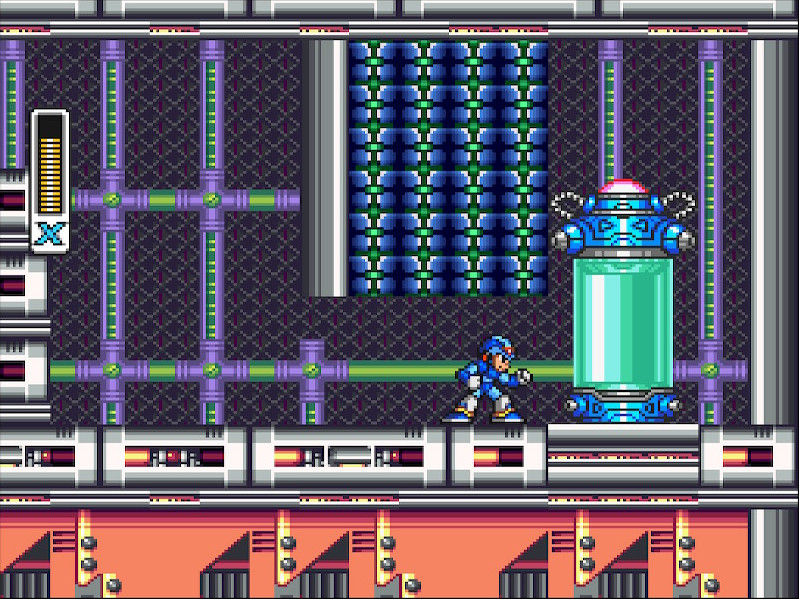
\includegraphics[width=0.5\textwidth]{figures/X1/Storm_eagle/Storm_armor_2.jpg}
		\caption{Head Part capsule location}
	\end{figure}
	
	\item Hadoken. While not being technically a component of the First Armor, rather an hidden bonus, this technique is stored too inside a Light's capsule so it is reported here. It allows X to perform the well-know technique from \textit{Street Fighter} by inputting the button combination $\downarrow$ $\searrow$ $\rightarrow$ (with X facing right) + fire button or using the same combination while X is charging and release the charged shot~\cite{RTA_wiki:X1}  AND X is at full health. The projectile deals 32 point of damage~\cite{wiki:Hadoken} to all enemies, basically one-shotting every non-shielded enemy, bosses included. The only exception is Sigma's final form, and only in the original \textit{Mega Man X}. 
	
	Both in the original game and its remake the capsule is hidden in Armored Armadillo Stage (see sec.~\ref{hadoken} for more information on how unlock it).
	\begin{figure}[htp]
		\centering
		\begin{subfigure}{0.3\linewidth}
			\centering
			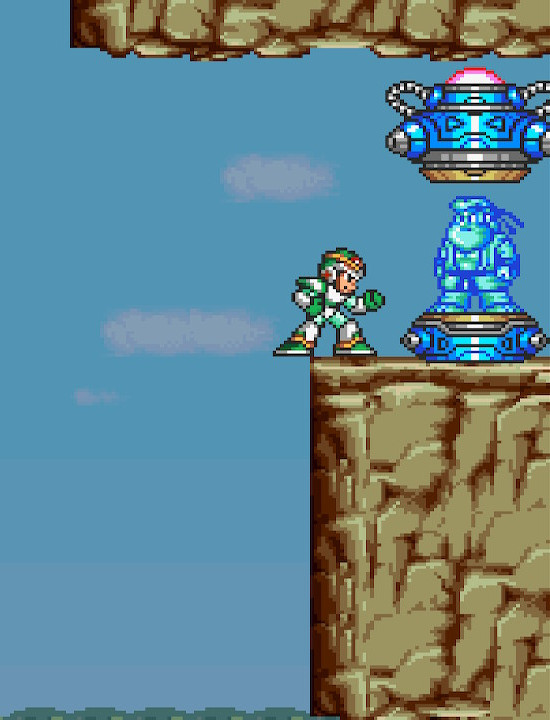
\includegraphics[width=\textwidth]{figures/X1/Armored_armadillo/Armadillo_hadoken.jpg}
		\end{subfigure}
		\begin{subfigure}{0.5\linewidth}
			\centering
			\includegraphics[width=\textwidth]{figures/X1/weapons/hadoken.jpg}
		\end{subfigure}
		\caption{hadoken Capsule location and technique}
	\end{figure}
	In any case the player has to keep in mind that, in the original game, this power-up isn't save by the password system, meaning that it has to be re-unlocked again if the game is restarted.
\end{itemize}

\section{Highway}
The Highway Stage (Central HighWay in \textit{Maverick Haunter X}) is the first stage of the game. X arrives here in order to join the fight against Sigma's forces.
 The stage is rather straightforward, having X to travel it while eliminating different enemies, and also teaching the player some basic mechanics such as wall-jumping.  The stage can be split into two main sections~\cite{stratwiki:HighWay}, the second one having more gaps and pieces of the highway falling as X stands on (recognizable by a darker texture color). In the first section of the highway two sub-bosses are presents in form of \hyperlink{miniboss:Bee_Blader}{Bee Blader}. At the end of the stage X will be attacked by the \hyperlink{veichle:Death_Rogumer}{Death Rogumer}, which will start sending towards him several \hyperlink{enem:Road_Attackers}{Road Attackers}.

 
 Once some of them have been destroyed, Vile will drop out the airship and start attacking X with his ride armor. Vile is literally invincible, so there is 
 no point in fighting. Instead as X drop below a certain amount of energy Vile will start shooting an energy projectile toward X and has soon as it connects, X gets trapped and the fight ends, starting the cutscene with Zero saving X. A common speedrun  technique involve having X getting hurt in order to start the boss fight with low health, which will force Vile to immediately shoot the trapping projectile and then run into it, basically skipping the entire fight.  Attention however has to be made, since Vile will not stop attacking with the armor, which may results in the player being defeated.
 
\begin{figure}[htp]
	\centering
	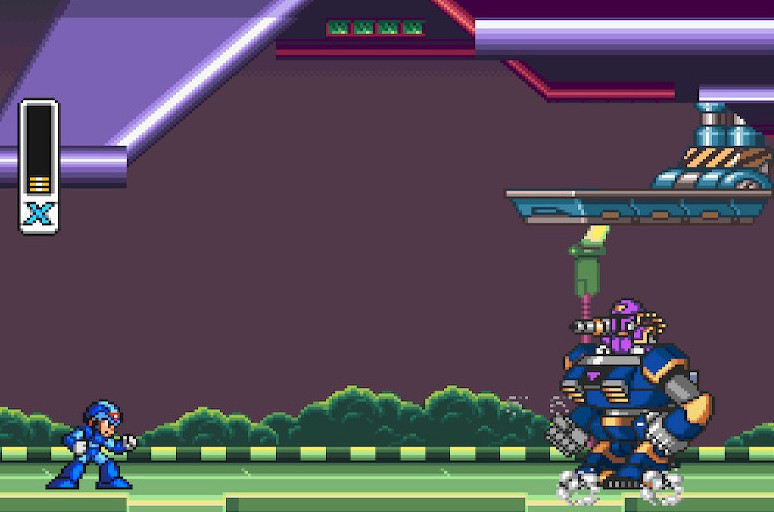
\includegraphics[width=0.5\linewidth]{figures/X1/Highway_screenshot.jpg}
	\caption{X facing Vile.}
\end{figure}
This stage contains following enemies~\cite{wiki:Highway}:
\begin{itemize}
	\item \hyperlink{enem:Ball_De_Voux}{Ball De Voux }
	\item \hyperlink{enem:Bomb_Been}{Bomb Been }
	\item \hyperlink{enem:Crusher}{Crusher }
	\item \hyperlink{enem:Gun_Volt}{Gun Volt}
	\item \hyperlink{enem:Jamminger}{Jamminger}
	\item \hyperlink{enem:Road_Attackers}{Road Attackers }
	\item \hyperlink{enem:Spiky}{Spiky }
	\item \hyperlink{miniboss:Bee_Blader}{Bee Blader }
\end{itemize}


Once finished the introduction stage the player will be presented with the classical boss selection screen typical of the Mega Man franchise, which allow the player to choose which boss face first. Here stages will be presented in order as they appear on the screen, from left to right, top to down.
\begin{figure}[htp]
	\centering
	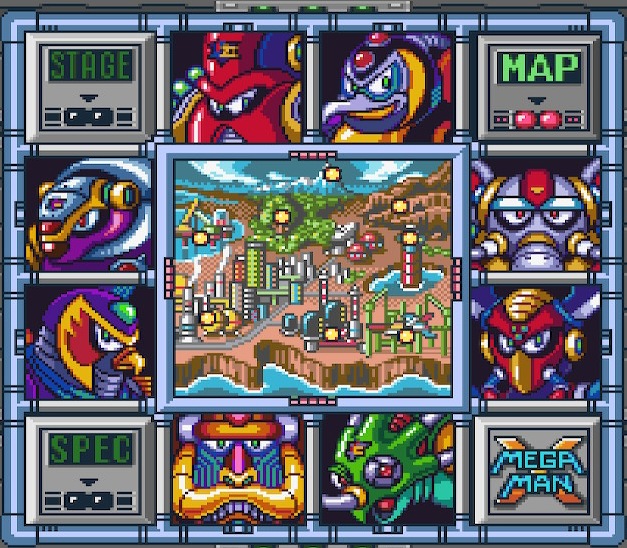
\includegraphics[width=0.5\linewidth]{figures/X1/Full_map.png}
	\caption{Full map with Bosses and their locations}
\end{figure}
 
 
 
\section{Ocean}
The \textit{Ocean stage} (later renamed Subterranean Base in \mhx) is where Launch Octopus hides himself. Here X starts from the shoreline to immerse underwater shortly after level's beginning. Once underwater X will jump higher than normal which, combined with dash-jump high reach and the beginning of the level being placed on top of a cliff, makes the player capable of skipping a good portion of stage's first part~\cite{stratwiki:Ocean}. Various fish-based enemies are present, but main difficulties comes the sub-bosses the stage has, being three plus an optional one. In the first part main difficulties are given by spiked pit which X has to jump and from where \hyperlink{enem:Sea_Attacker}{Sea Attacker} will spawn in group of three, interrupting X's jump and making him fall into the pit, and from the two \hyperlink{miniboss:Anglerge}{Anglerge} sub-bosses, the second one being particular dangerous, since the floor has two spiked pits and the Anglerge will keep using his vacuum attack to push/pull X into them. Here the best strategy consists in stay at the leftmost platform and keep shooting, dashing to the right once it start pulling and shooting while it pushes X. Other than that Anglerges will also shoot X four serpent-shaped harpoon which will move horizontally and then fall'rise onto X when they're above/below him. Finally Anglerges will rarely shoot a beam of light from their lamp, which can also be destroyed. After passing the second sub-boss the second part of the stage begins. Here spiked gaps are rarer (although still present) and whirlpools will start to appear at regular intervals and in specific positions. Those whirlpools can be used to propel X up to the ocean's surface. Proceeding in the stage bombs will start dropping from above, fired by a \hyperlink{miniboss:Cruiziler}{Cruiziler} enemy. X can either climb a whirlpool to get onto it and destroy its core, making it sink and stop it from shooting bombs, or avoiding it and proceed in the level. Once passed falling bombs, X will find himself into an arena filled with sand. Here an \hyperlink{miniboss:Utuboros}{Utuboros} will start attacking him, rising from the sand, than swimming for a while and then immerse again in the sand. It is invincible for most of its body (which X can stand on), only the head and tail being vulnerable. Although its weakness is considered to be the Boomerang Cutter, due to lack of invincibility frame a single Storm Tornado fired behind its head will destroy him in one shot~\cite{wiki:Utuboros}. After this other sub-boss X will have go forward on only for a little before finding himself in front of the boss door.

Here is a list of all enemies present in the stage~\cite{wiki:Ocean}:
\begin{itemize}
	\item \hyperlink{enem:Amenhopper}{Amenhopper}
	\item \hyperlink{miniboss:Anglerge}{Anglerge}
	\item \hyperlink{miniboss:Cruiziler}{Cruiziler}
	\item \hyperlink{enem:Gulpfer}{Gulpfer }
	\item \hyperlink{enem:Mega_Tortoise}{Mega Tortoise }
	\item \hyperlink{enem:Sea_Attacker}{Sea Attacker}
	\item \hyperlink{enem:Sky_Claw}{Sky Claw }
	\item \hyperlink{miniboss:Utuboros}{Utuboros}
\end{itemize}

\subsection{Heart Tank}
This stage only has an heart tank has its collectible. In order to get it the player musts first destroy the Cruizer by reaching the ocean's surface via the closest whirlpool, climbing it and then shooting Cruizer's blue core, avoiding in the meanwhile the Sky Claws which the ship will spawn. Once destroyed, the Cruizer will sink and will destroy the ocean's floor, revealing an hidden portion with a large room filled with spiked gaps on the ground. Here another Utuboros (technically the first since the other reside later in the level) must be defeated, in order to open the door which leads to an Heart Tank. After that X must exit from where he entered and climb the wall where the ship fall in order to return to the main path.
\begin{figure}[htp]
	\centering
	\begin{subfigure}{0.37\textwidth}
		\centering
		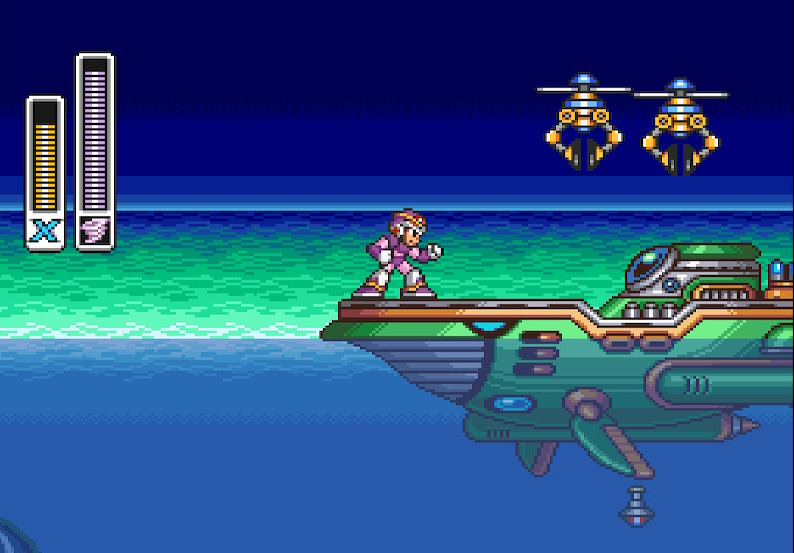
\includegraphics[width=\linewidth]{figures/X1/Launch_octopus/Octopus_heart_1.jpg}
		\caption{}
	\end{subfigure}
	\begin{subfigure}{0.4\textwidth}
		\centering
		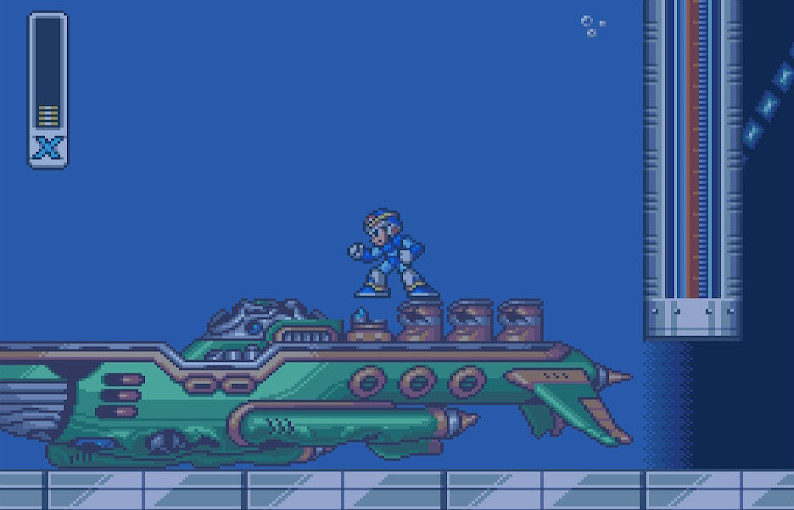
\includegraphics[width=\linewidth]{figures/X1/Launch_octopus/Octopus_heart_2.jpg}
		\caption{}
	\end{subfigure}\\
	\begin{subfigure}{0.4\textwidth}
		\centering
		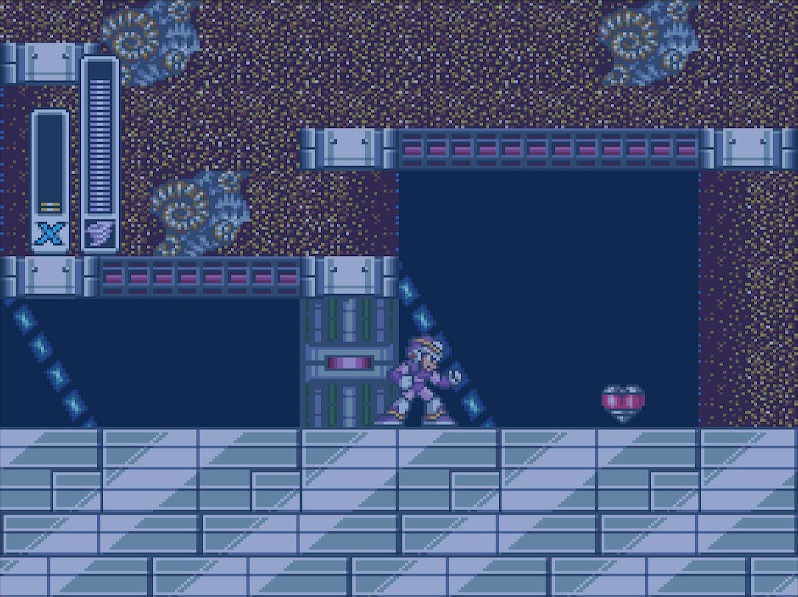
\includegraphics[width=\linewidth]{figures/X1/Launch_octopus/Octopus_heart_3.jpg}
		\caption{}
	\end{subfigure}
	\caption{(a)Via whirlpool the player can reach the Cruizer on ocean's surface,(b) When destroyed the ship will fall down, breaking the ocean floor and opening a new path,(c) One destroyed the Utuboros inside the cave, a room will open with the Heart Tank inside}
\end{figure}

\subsection{Launch Octopus}\label{boss:Launch_octopus}
\begin{figure}[htp]
	\centering
	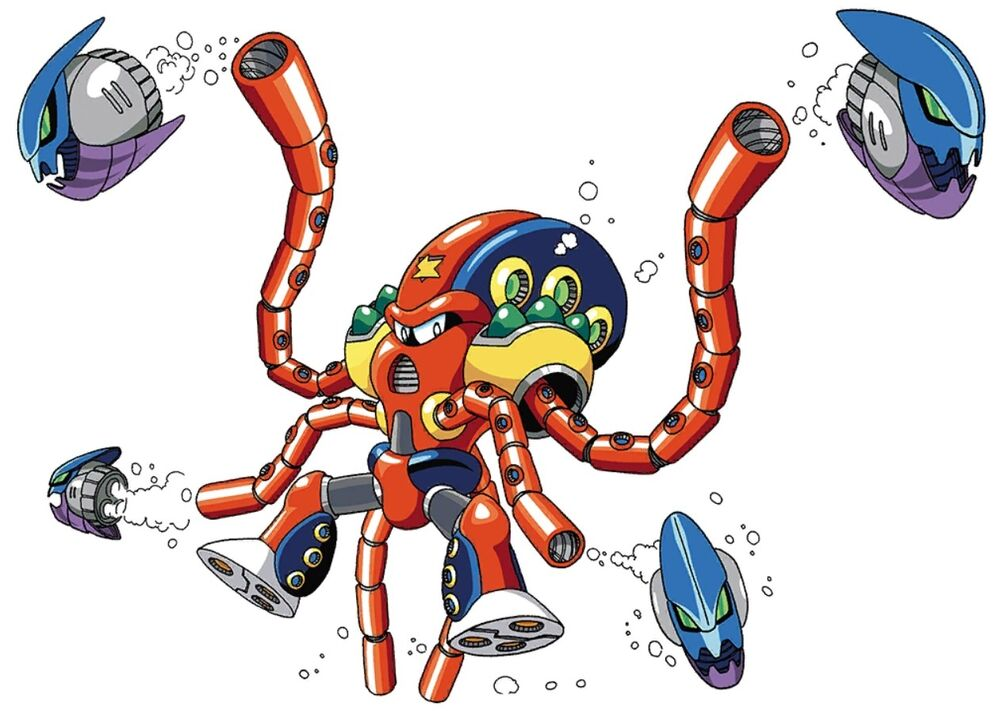
\includegraphics[width=0.5\linewidth]{figures/X1/Launch_octopus/LaunchOctopus.jpg}
	
\includegraphics[width=0.4\linewidth]{figures/X1/Launch_octopus/MHXLaunchOctopus.jpg}
	\caption{Launch Octopus' designs (\cite{book:MMX_Complete_art})}
\end{figure}

Launch Octopus, the ``\textit{General of the Deep Sea}''~\cite{book:MMX_Complete_art} was a Maverick Haunter of the 6th Fleet armada before joining Sigma's rebellion and setting his base in the dept of the Ocean, in order to attack marine cities with his army of mechaniloids and to cut off shipping routes. In \x he joins Sigma due the fact he shares the dream of a world only for reploids, having always doubt about protecting humans, while in \mhx he is pictured military tactician which want to achieve beauty in combat, considering himself an unappreciated artist of underwater fighting. Only Sigma understand his art, making Launch Octopus side with him~\cite{wiki:MM_MHX_script}.

\begin{figure}[htp]
	\centering
	\begin{subfigure}{0.48\textwidth}
		\centering
		\includegraphics[width=\linewidth]{figures/X1/Launch_octopus/Octopus_missile.jpg}
		\caption{Homing Torpedo}
	\end{subfigure}
	\begin{subfigure}{0.49\textwidth}
		\centering
		\includegraphics[width=\linewidth]{figures/X1/Launch_octopus/Octopus_piranha.jpg}
		\caption{Charged Homing Torpedo}
	\end{subfigure}
	\end{figure}

	\begin{figure}
	\ContinuedFloat
	\centering
	\begin{subfigure}{0.2\textwidth}
		\centering
		\includegraphics[width=\linewidth]{figures/X1/Launch_octopus/Octopus_vortex.jpg}
		\caption{Vortex}
	\end{subfigure}
	\begin{subfigure}{0.37\textwidth}
			\centering
			\includegraphics[width=\linewidth]{figures/X1/Launch_octopus/Octopus_drain.jpg}
			\caption{Energy Drain}
	\end{subfigure}
	\begin{subfigure}{0.39\textwidth}
		\centering
		\includegraphics[width=\linewidth]{figures/X1/Launch_octopus/Octopus_cut.jpg}
		\caption{Tentacles cut off}
	\end{subfigure}
	
	\caption{Launch Octopus' attacks}

\end{figure}

In battle Octopus has two main techniques: Homing torpedo and Energy Drain. In reality he has a third technique, which consists in firing what can be considered a charged version of his Homing Torpedo. Both his types of missiles can be destroyed by shooting at them. Launch Octopus will always start the boss fight with a barrage of homing missile, to than  switch to one of the other two weapons he has. Just like X, Octopus can fire a charged version of his homing missiles, which are piranha-shaped and homes much faster than their counterpart. Finally he has his Energy Drain attack. When performing this Octopus will first swim on top of the arena, either left or right, and then start spinning to create a whirlpool to suck X in. If he succeeds he will start draining X energy to replenish his own, prolonging the fight until the player breaks free. Octopus main weakness is the Rolling Shield, which deals him extra damage but can be hard to hit, due Octopus high mobility and the shield colliding with his missiles instead. However Octopus can be also heavily damaged by the Boomerang Cutter, which in three hits will sever his tentacles blocking him to perform his Energy Drain attack. 


Officially~\cite{wayback:X_resources} Launch Octopus is 232 cm tall and 182 Kg heavy, in contrast with in-game information~\cite{wiki:Launch_octopus} which show a weight value smaller than actual ones (see fig ~\ref{Octopus_specs}).

Oncee Launch Octopus has been defeated X will gain the Homing Torpedo (\ref{Homing_torpedo}) weapon, as well as cause a flood in the Forest Stage, making water appear near the beginning of the stage.
\begin{figure}[htp]
	\begin{minipage}[c]{0.45\linewidth}
		\vspace{0pt}
		\centering
		\includegraphics[width=\linewidth]{figures/X1/Launch_octopus/Launch_octopus_specs.png}
	\end{minipage}
	\begin{minipage}[c]{0.45\linewidth}
		\centering
		\vspace{0pt}
		\begin{tabular}[h]{l c}
			\toprule
			Health Bar & 32\\
			\midrule
			\multicolumn{1}{c}{Attack} & \multicolumn{1}{c}{Damage}\\
			Contact & 4\\
			Homing Torpedo & 2\\
			Charged H. Torpedo & 2\\
			Energy Drain & 1-15\\
			\bottomrule
		\end{tabular}
	\end{minipage}
	\caption{Left: Launch Octopus' specifications and according to X1; Right: In-game data~\cite{wiki:Launch_octopus}. }
	\label{Octopus_specs}
\end{figure}


\section{Snow Mountain}
\textit{Snow Mountain}(\textit{Abandoned Missile Base in \mhx}) is probably the first stage most people go when starting the game, due to its low level of danger it contains~\cite{stratwiki:Snow_mountain}, as for having inside the most useful upgrade X get can get, the Foot Parts. The stage, as the name states, takes place in a snow-covered mountain which X has to climb to get to the boss. The stage is divided into three main areas. The first area is where X starts and consists in a path that brings him inside a cave through a series of enemies. Once inside the cave (the second area) X has first to climb it by following a zig-zag path while also avoiding enemies which drop from higher level, and then to surpass some iced platform separated by pits until he reaches the end of the cave. In the third area X is again on the outside. Here he can take a Ride Armor and proceed for a while. With the armor X can also destroy the igloo he finds and that would otherwise start spawning enemies. Passed the first igloo a choice can be made: to keep the Ride Armor and enter the small cave which comes next, where it is request to jump some gaps using the armor while also face another enemy Ride Armor, or use the armor to reach the top of the cave (jumping out of the armor to gain extra lift), basically skipping the lower portion. After that section X meets a tall wall which the armor cannot surpass, forcing him to leave it behind. Here he has to following a path full of slopes, gaps and \hyperlink{enem:Snow_Shooter}{Snow Shooters}, which will throw snowballs at him and that become bigger the longer they roll on the snowy ground. After passing these enemies, the player will reach the boss door.

The stage contains following enemies~\cite{wiki:Snow_mountain}:
\begin{itemize}
	\item \hyperlink{enem:Armor_Soldier}{Armor Soldier} (with Ride Armor)
	\item \hyperlink{enem:Axe_Max}{Axe Max}
	\item \hyperlink{enem:Batton_Bone}{Bat Bone}
	\item \hyperlink{enem:Bomb_Been}{Bomb Been}
	\item \hyperlink{enem:Flammingle}{Flammingle}
	\item \hyperlink{enem:Jamminger}{Jamminger }
	\item \hyperlink{enem:Ray_Bit}{Ray Bit}
	\item \hyperlink{enem:Snow_Shooter}{Snow Shooter}
	\item \hyperlink{enem:Spiky}{Spiky}
	\item \hyperlink{enem:Tombot}{Tombot}
\end{itemize}

\subsection{Light's Capsule}\label{X:Foot_Parts}
In Mega Man X this stage contains the Armor capsule for the Foot Parts, which allows X to dash, also allowing to perform dash-jumps and wall dash-jumps. Furthermore dashing also reduce a little X's height and hitbox, allowing do dodge certain attacks by dashing beneath them. The capsule is found directly onto the main path after climbing the first part of the cave. Since it is right in the middle of the path it is not avoidable, making it the only mandatory capsule of the entire series.
\begin{figure}[htp]
	\centering
	\includegraphics[width=0.5\textwidth]{figures/X1/Chill_penguin/Armor_foot.jpg}
	\caption{Foot Part capsule location}
\end{figure}

In the remake \mhx, instead, this stage hides the Head Parts. The capsule is hidden in the first indoor climbing section, hide by block breakable only via Foot Parts.
\subsection{Heart Tank}\label{Penguin:heart_tank}
The Heart Tank of this stage is hidden in the last igloo X meet before facing the section with snow balls. To reach it X has to jump using the Ride Armor. After the first igloo there is a light blue column, right before the cave with the enemy Ride Armor. From the top of the column the player has to jump with the armor and, once reached the maximum height, jump out of it in order to reach the wall which brings to the upper path. Here two other igloo are found which can be destroyed, now that the armor is gone, by using the Fire Wave weapon. In particular the last one contains the searched Heart Tank.
\begin{figure}[htp]
	\centering
	\begin{subfigure}{0.375\linewidth}
		\centering
		\includegraphics[width=\textwidth]{figures/X1/Chill_penguin/Chill_heart_1.jpg}	
		\caption{}
	\end{subfigure}
	\begin{subfigure}{0.4\linewidth}
		\centering
		\includegraphics[width=\textwidth]{figures/X1/Chill_penguin/Chill_heart_2.jpg}	
		\caption{}
	\end{subfigure}
	\caption{Heart Tank location.}
\end{figure}

\subsection{Chill Penguin}\label{boss:Chill_Penguin}
\begin{figure}[htp]
	\centering
	\includegraphics[width=0.5\linewidth]{figures/X1/Chill_penguin/Chill_Penguin.jpg}
	\includegraphics[width=0.4\linewidth]{figures/X1/Chill_penguin/MHXChillPenguin.jpg}
	\caption{Chill Penguin's designs (~\cite{book:MMX_Complete_art})}
\end{figure}

The ``\textit{Glacial Emperor}''~\cite{book:MMX_Complete_art}, better known as Chill Penguin was a reploid of the 13th Polar Division, specifically designed for operating in polar environments also tanks to his small-size body. However due to the long permanence in the South Pole, away from civilization, Chill Penguin grown tired of his mission, seeking a way to get away from there. Sigma's rebellion give him exactly what he needed to return to the civilization, allowing him to escape and join Sigma in his fight. There are however some differences in how his story is told between \x and \textit{Maverick Haunter X}. In the former, after Sigma starts his revolt, Chill Penguin autonomously eliminated his own commander and escaped to join Sigma~\cite{Xcoll1:Manual_X1}, seizing a mountain base in order to crush nearby cities using avalanches. Meanwhile in the remake it is Sigma himself which took away Chill Penguin from the South Pole by making him join the 17th division together with X and Zero, even before the revolution's beginning~\cite{MHX:manual}. Later, while facing X, Chill Penguin reveals that, beside to leave the South Pole, he also joined the revolt due the payment Sigma gave him~\cite{wiki:MMX_script}. Another minor difference with the original version is that, in the remake, Chill Penguin seized an abandoned missile base, hinting his purpose was to use it to attack the cities. 

According to descriptions, Chill Penguin is known to be a belligerent, rowdy (sometimes even warped) individual, while also having trouble with his partner Flame Mammoth (\ref{boss:Flame_mammoth}) due his jealously of Mammoth size and the latter attitude of bullying smaller reploids.


Chill Penguin is often considered the easiest boss of the game and the first one a player should face due the simplicity of avoiding his attacks, also thanks to the Foot Parts the stage give to the player. He has four main attack which will perform at random~\cite{wiki:Chill_Penguin}. When he use his Shotgun Ice, Chill Penguin will shot four frozen projectiles which travel in a straight line, although some of them  can fall off and slide on the ground, which shatter upon contact with a wall but can nullify X's shots if the two met. Other times instead of his projectiles he will emit a snowy breath which will create two penguin-shaped ice sculpture and, if X is in range, will also freeze him in place. Sculptures act both as obstacles (X takes damage if he makes contact with them) and as covers since both X and Chill Penguin projectiles will be stopped by them, but can be destroyed if enough damage are dealt to them.
\begin{figure}[htp]
	\centering
	\begin{subfigure}{0.44\textwidth}
		\centering
		\includegraphics[width=\linewidth]{figures/X1/Chill_penguin/Chill_shot.jpg}
		\caption{Shotgun Ice}
	\end{subfigure}
	\begin{subfigure}{0.53\textwidth}
		\centering
		\includegraphics[width=\linewidth]{figures/X1/Chill_penguin/Chill_frozen.jpg}
		\caption{X frozen near two ice statues}
	\end{subfigure}
	\begin{subfigure}{0.5\textwidth}
		\centering
		\includegraphics[width=\linewidth]{figures/X1/Chill_penguin/Chill_shatter.jpg}
		\caption{Chill Penguin's shotgun ice stopped by his own statues}
	\end{subfigure}
	\begin{subfigure}{0.4\textwidth}
		\centering
		\includegraphics[width=\linewidth]{figures/X1/Chill_penguin/Chill_slide.jpg}
		\caption{Slide attack}
	\end{subfigure}
	\begin{subfigure}[t]{0.5\textwidth}
		\centering
		\includegraphics[width=\linewidth]{figures/X1/Chill_penguin/Chill_blizzard.jpg}
		\caption{Blizzard attack}
	\end{subfigure}
	\begin{subfigure}[t]{0.35\textwidth}
		\centering
		\includegraphics[width=\linewidth]{figures/X1/Chill_penguin/Chill_burn.jpg}
		\caption{Chill Penguin is burnt by the Fire Wave}
	\end{subfigure}
	\caption{Chill Penguin's attacks}
\end{figure}
In some occasion Chill Penguin will leap in the air and grab the hook on the ceiling, unleashing a blizzard which will push X and the statues (if present) against a wall, causing sculptures to shatter in the process. Finally he can also slide on the floor for a while, turning immediately in case he hits a wall. While in this state he is invincible, but will also get rid the sculpture he creates.  As it is possible to see, Chill Penguins attacks only cover the low part of the arena, meaning the best strategy to fight him consist in staying on the higher part via continuous wall-jumps, only dropping to hit him when possible. Attention however must be made, since sometimes Chill Penguin will perform a high jump toward X position which can hit him even if he's  in the high corner of the room. Beside that he can be hit at any times, even when grabbing the hook, beside when sliding. He's weakness is the Fire Wave, which will burn and stun him for a while, but it has no other particular effect.

After defeating him X will gain the Shotgun Ice (\ref{Shotgun_ice}) weapon as well as freezing the lava in the Factory Stage, considerably reducing the danger level of the stage.

Chill Penguin is 163 cm tall and 108 Kg heavy, despite the information screen on the game report different (\ref{Penguin_specs}).

\begin{figure}[htp]
	\begin{minipage}[c]{0.45\linewidth}
		\vspace{0pt}
		\centering
	\includegraphics[width=\linewidth]{figures/X1/Chill_penguin/Chill_penguin_specs.jpg}
	\end{minipage}
	\begin{minipage}[c]{0.45\linewidth}
		\centering
		\vspace{0pt}
		\begin{tabular}[h]{l c}
			\toprule
			Health Bar & 32\\
			\midrule
			\multicolumn{1}{c}{Attack} & \multicolumn{1}{c}{Damage}\\
			Contact & 6\\
			Shotigun Ice & 2\\
			Ice Breath & 0\\
			Ice statue & 4\\
			Sliding & 6\\
			\bottomrule
		\end{tabular}
	\end{minipage}
	\caption{Left: Chill Penguin's specifications and according to X1; Right: In-game data~\cite{wiki:Chill_Penguin}. }
	\label{Penguin_specs}
\end{figure}


\section{Gallery}
The Gallery Stage (or Energy Mines Ruins in \mhx) is the stage controlled by Armored Armadillo. Peculiarity of this level are its mine carts on which X can stand and, as soon as he does it, they start moving following the track, increasing their speed as they keep going and destroying all enemies that enter in contact with them. Hoever the player must be careful, as all the carts end their run into pits, bringing X down with them if he doesn't jump off at the right moment. This stage is also famous for containing the secret Light's capsule which teach X the hadoken technique, as well as being the best place to farm health capsule and lives.

The stage itself is rather simple. Immediately at the beginning a mine cart is present which brings the player forward in the level while also taking care of enemies, but that end its ride when it comes across a series of gaps, one of which it cannot jump and falls into. For that moment the player must have dismounted from the cart. After this sequence only few small gaps and some enemies separate X from the next section, which begin when he has to fall off a long pit in the ground. Here as he touches the floor a \hyperlink{miniboss:Mole_Borer}{Mole Borer} will destroy the left wall and start chasing X. This enemy is invincible and its roller can insta-kill X if he touches it, so only two solutions are possible: the first one is to escape to the right, continuing in the level; the second one is, as soon as X reaches the ground, wall jump immediately to the left before the Mole Borer breaks the wall and then jump down, following it from behind (while also gaining acces to the sub tank). In both cases the player has to go right to continue, followed by the mechaniloid (which will eventually crash and explode) or behind it. After this section another mine cart waits, which will bring the player deeper in the level to end, again, its ride into a pit. Just like the previous section, after this part too ends with large hole in the ground X has to fall off to proceed, meeting another Mole Borer once he lands. This time however he will land behind it, avoiding another chase and, on the other hand, allow the mechanilod to create a passage for the player, until it crashes and explodes again (the player may also want to destroy it since while going it also destroys the access to the heart tank). Here there is the final cart X has to take to proceed. This mine cart brings X through many enemies until it reaches an opening on the mountain and flies off over a huge gap, impossible for X to jump. Once in the air the player must jump off the cart in order to land on the other side of the pit (or grab the wall if high enough), where the boss door is. While riding in the final parts a group of mechanical birds enemies will start spawning and fly alongside X. Since they fly the cart cannot destroy them, but X will have to, since they can mess up the final jump by hitting him and making him fall into the pit.

Following enemies are present in the stage~\cite{wiki:Gallery}:
\begin{itemize}
	\item \hyperlink{enem:Batton_Bone}{Bat Bone} 
	\item \hyperlink{enem:Batton_M-501}{Batton M-501} 
	\item \hyperlink{enem:Dig_Labour}{Dig Labour} 
	\item \hyperlink{enem:Flammingle}{Flammingle} 
	\item \hyperlink{enem:Metal_Wing}{Metal Wing} 
	\item \hyperlink{enem:Metall_C-15}{Metall C-15} 
	\item \hyperlink{miniboss:Mole_Borer}{Mole Borer}
	\item \hyperlink{enem:Spiky}{Spiky}
\end{itemize}
\begin{figure}[htp]
	\centering
	\includegraphics[width=0.5\linewidth]{figures/X1/Armored_armadillo/Armadillo_tank.jpg}
	\caption{Gallery stage's subtank location}
\end{figure}
\subsection{Sub Tank}
This stage's Sub Tank is located where the first Mole Borer appears. In order to get it the player has, once arrived to the firs big gap in the ground, jump into it and then immediately wall-jump to the left, in order to let the Mole Borer break the wall and go right passing under X. Once it is passed, the player can safely jump off and go left to find the sub tank where the Mole Borer originally was. 


\subsection{Heart Tank}
The heart tank is located near where the second Mole Borer is found. Once  X jumps off the gap he has to chase the mechaniloid and destroy it in time, since as it proceeds it will destroy walls which allow to access the Heart Tank. To do this the Fire Wave weapon is suggested, since it deals massive amount of damage to it in a short amount of time. 
\begin{figure}[htp]
	\centering
	\begin{subfigure}{0.3\linewidth}
		\centering
		\includegraphics[width=\linewidth]{figures/X1/Armored_armadillo/Armadillo_heart.jpg}
		\caption{}
	\end{subfigure}
	\begin{subfigure}{0.3\textwidth}
		\centering
		\includegraphics[width=\linewidth]{figures/X1/Armored_armadillo/Armadillo_heart_2.jpg}
		\caption{}
	\end{subfigure}
	\caption{Gallery stage's heart tank location. In (a) the Mole Borer has been destroyed and X can wall jump and reach it, while in (b) the Mole Borer has passed and X cannot reach the opening anymore}
\end{figure}

\subsection{Hadoken}\label{hadoken}
The hadoken is the last upgrade X can get before facing finals stages. The capsule containing it can be unlocked only of the player has managed to collect every other upgrade in the game: eight Heart Tanks, four Sub-Tank, four armor capsule and all the weapon from bosses. Next the player has to travel trough the gallery stage and reach the top of the ledge above the boss door at least three time after defeating Armored Armadillo. At the fourth time, if the player manages to reach the place at full health, near the usual health drop there will also be the secret capsule.
\begin{figure}[htp]
	\centering
	\includegraphics[width=0.3\linewidth]{figures/X1/Armored_armadillo/Armadillo_hadoken.jpg}
	\caption{hadoken capsule with Dr.Light in Ryu's attire.}
\end{figure}
The best way to make the capsule spawn is as follow: As the stage begin, the player has to travel the level (by walking or on the mine cart) unit it reaches the zone where a single \hyperlink{enem:Batton_M-501}{Batton M-501} drops from the roof (near the first Flammingle). Here the player should farm lives by continuing killing that enemy (which has a increased drop rate for them)  and making it respawn by walking away and returning (it is suggest to use a charged Rolling Shield as it destroys it in one hit). After having accumulated enough lives (at leas five) the player can proceed in the level until the last mine cart is reached, making sure to be at full health by this point. Here X has first to release a charged Sting Chameleon and immediately after ride the cart until over the pit, where he should jump off and grab the ledge over the boss door, reaching the top of if. As X reaches it, he has to jump into the pit, loosing a life and respawning at the last checkpoint (before the second Mole Borer). From here the player has to repeat this procedure for other three times until, at the  fourth one, the capsule will be there. In the remake the capsule does not require multiple travel through the stage, being available immediately.

Once opened the capsule will reveal Dr. Light wearing robe similar to Ryu's one from the Street Fighter series, which will ask X to step into the capsule to teach him the technique. In the Japanese  script of the game~\cite{wordpress:X_japanese_script} Light states that he trained under the nearby waterfall a lot to learn it, and that he will now teach it to X who can learn it, as stated again by Light himself in the remake, due to him having a nearly-human soul.


\subsection{Armored Armadillo}\label{boss:Armored_Armadillo}
\begin{figure}[htp]
	\centering
	\includegraphics[width=0.3\linewidth]{figures/X1/Armored_armadillo/Armored_armadillo.jpg}
	\includegraphics[width=0.4\linewidth]{figures/X1/Armored_armadillo/MHXArmoredArmadillo.png}
	\caption{Armored Armadillo's designs (~\cite{book:MMX_Complete_art})}
\end{figure}
Armored Armadillo was the commander in charge of the 8th armored force, as well as a soldier loyal to his superior, Sigma. Once the latter started his revolt, Armored Armadillo blindly followed his orders, occupying a mine to extract raw materials from which Sigma aims to create weapons for his plans.

Faithful to his name and title (``\textit{Armored Warrior}''~\cite{book:MMX_Complete_art}) Armored Armadillo fights by using his impenetrable armor both as a shield to deflect X shots and as a weapon to crush him while using his main attack, the Rolling Shield, which see him turning into a ball and start bouncing off arena's walls while also being immune to any attack. In some occasion Armadillo will also take out the cannon hidden in his forehead and start shooting a sequence of rapid bullet in a straight line before beginning to roll again. 
\begin{figure}[htp]
	\centering
	\begin{subfigure}[t]{0.3\textwidth}
		\centering
		\includegraphics[width=\linewidth]{figures/X1/Armored_armadillo/Armadillo_rolling.jpg}
		\caption{Rolling Shield}
	\end{subfigure}
	\begin{subfigure}[t]{0.4\textwidth}
		\centering
		\includegraphics[width=\linewidth]{figures/X1/Armored_armadillo/Armadillo_cannon.jpg}
		\caption{Cannon}
	\end{subfigure}	
	\begin{subfigure}{0.35\textwidth}
		\centering
		\includegraphics[width=\linewidth]{figures/X1/Armored_armadillo/Armadillo_energy_1.jpg}
		\caption{Absorbing a charged shot}
	\end{subfigure}
	\begin{subfigure}{0.42\textwidth}
		\centering
		\includegraphics[width=\linewidth]{figures/X1/Armored_armadillo/Armadillo_energy_2.jpg}
		\caption{Releasing the energy}
	\end{subfigure}
\end{figure}
\begin{figure}[htp]
	\ContinuedFloat
	\centering
	\begin{subfigure}[t]{0.4\textwidth}
		\centering
		\includegraphics[width=\linewidth]{figures/X1/Armored_armadillo/Armadillo_shock_1.jpg}
		\caption{Armadillo hit by the Electric Spark}
	\end{subfigure}
	\begin{subfigure}[t]{0.4\textwidth}
		\centering
		\includegraphics[width=\linewidth]{figures/X1/Armored_armadillo/Armadillo_shock_2.jpg}
		\caption{Armor broken}
	\end{subfigure}\\
	\caption{Armored Armadillo's attacks.}
\end{figure}
Finally Armored Armadillo can also guard X's attacks, which makes him invincible and, moreover, he allows him also absorb and re-release charged shot which X fired at him.  

The main difficulty in facing Armored Armadillo is given mainly by the few time he leaves open himself to hits before turning invincible and start attacking again. To solve this problem his weak point comes in play. Armored Armadillo is in fact extremely weak to the Electric Spark since not only this weapon deals him more damage than others but it also can remove his plating. Once deprived of his armor, Armadillo won't be able to guard himself anymore and will also lost his invincibility while rolling, basically making the fight much easier for the player to manage.

Upon beating Armored Armadillo X gains the Rolling Shield weapon (\ref{Rolling_shield}), but no other effects take place in other stages.

According information give, Armored Armadillo is 194 cm tall and 232 kg heavy, while in-game information report him slightly smaller and lighter (\ref{Armadillo_specs}).
\begin{figure}[htp]
	\begin{minipage}[c]{0.45\linewidth}
		\vspace{0pt}
		\centering
		\includegraphics[width=\linewidth]{figures/X1/Armored_armadillo/Armored_armadillo_specs.png}
	\end{minipage}
	\begin{minipage}[c]{0.45\linewidth}
		\centering
		\vspace{0pt}
		\begin{tabular}[h]{l c}
			\toprule
			Health Bar & 32\\
			\midrule
			\multicolumn{1}{c}{Attack} & \multicolumn{1}{c}{Damage}\\
			Contact & 6\\
			Rolling Shield& 6\\
			Guarding & 6\\
			Head Beam & 4\\
			\bottomrule
		\end{tabular}
	\end{minipage}
	\caption{Left: Armored Armadillo's specifications and according to X1; Right: In-game data~\cite{wiki:Armored_Armadillo}. }
	\label{Armadillo_specs}
\end{figure}


\section{Factory} 
The \textit{Factory Stage} (\textit{Prototype Weapons Plant} in \mhx)  is probably one of the most difficult stage among the eight, due to the high number of danger X can met and that can kill him instantly. The level takes place inside a factory which has been designated to weapons production, as the numerous conveyor belts, presses, and molten metal suggest and that X must face before reaching the boss. However if X manages to defeat Chill Penguin before entering the level, he will found the metal frozen solid, reducing considerably the danger level of the area, as he can stands on it whether he falls from a conveyor belt.
\begin{figure}[h]
	\centering
	\begin{subfigure}{0.49\textwidth}
		\centering
		\includegraphics[width=\linewidth]{figures/X1/Flame_mammoth/Flame_fire.jpg}
		\caption{}
	\end{subfigure}
	\begin{subfigure}{0.465\textwidth}
		\centering
		\includegraphics[width=\linewidth]{figures/X1/Flame_mammoth/Flame_frozen.jpg}
		\caption{}
	\end{subfigure}\\
	\caption{Factory Stage before (a) and after (b)  defeating Chill Penguin}
\end{figure}

The stage can be divided into four parts. At the beginning two sets of conveyor belt are present over molten metal which will try to obstacle his movement, together with  \hyperlink{enem:Scrap_Robo}{Scrap Robos} which will keep spawning on them and that will try attack X by crawling at him or by shooting lasers. At the end of this section X has to jump off a hole into the ground which brings him deeper into the factory. The next section is where all level's power-up are concentrated. It consists in a single big room, again on top of molten metal, without conveyor belts but with multiple platform at different heights from which enemies will attack X throwing down their pickaxes. The main danger here is given by the trajectory of the pickaxes since, being parabolic, allow them to be throw safely from upper levels (eventually even from off-screen) without giving X the chance to fire back until he reaches the same platform the enemy stands on. Reached the exit of this part on the top right of the room, another section with conveyor belts and Scrap Robo is present, this time with the addition of presses which insta-kill X if he gets caught. Finally the last part of the stage sees X walking on pipes. Here dangers comes from molter iron dripping from pipes, although it only damages X,  \hyperlink{enem:Rolling_Gabyoall}{Rolling Gabyoalls} which move along pipes while also flipping up and down and finally \hyperlink{enem:Hoganmer}{Hoganmers}, enemies which can be hit only when attacking (as they lower their shield) or by attacking them from behind. In this section some ladders are present, but their only purpose it to create side-paths to skip enemies and their utility is questionable. At the end of this section there is the boss door which leads to Flame Mammoth.

These enemies appears in this stage~\cite{wiki:Factory}:
\begin{itemize}
	\item \hyperlink{enem:Dig_Labour}{Dig Labour} 
	\item \hyperlink{enem:Hoganmer}{Hoganmer}
	\item \hyperlink{enem:Metall_C-15}{Metall C-15}
	\item \hyperlink{enem:Scrap_Robo}{Scrap Robo}
	\item \hyperlink{enem:Sky_Claw}{Sky Claw}
	\item \hyperlink{enem:Rolling_Gabyoall}{Rolling Gabyoall}
\end{itemize}

\subsection{Light's Capsule}
At the entrance of the big room the player will notice some blocks on the roof which can be broke with the Head parts. In order to do so the player has to dash-jump to the left from the very end of the first platform in order to make X destroy rightmost block, which will allow him to wall-jump on the remaining one. Once X has started wall jumping the player has to keep going, in order to climb while destroying remaining blocks and then to access the capsule with the Arm Parts. It is a very precise jump, so many tries can be needed. Furthermore it is possible for X to destroy the block but not starting to wall jump, falling on the ground. This complicates the situation, since the jump now is even more difficult, but still doable, requiring enough precision to make X land on the remaining block at sufficient height to start a wall jump. If for some reasons the player destroy the second block too the climb became impossible and the player has to kill himself to reset the area.
\begin{figure}[h]
	\centering
	\begin{subfigure}{0.3\textwidth}
		\centering
		\includegraphics[width=\linewidth]{figures/X1/Flame_mammoth/Flame_armor_1.jpg}
		\caption{}
	\end{subfigure}
	\begin{subfigure}{0.4\textwidth}
		\centering
		\includegraphics[width=\linewidth]{figures/X1/Flame_mammoth/Flame_armor_2.jpg}
		\caption{}
	\end{subfigure}\\
	\caption{Buster upgrade position: a dash-jump is required from (a) to to start wall-jumping and break the ceiling to reach (b).}
\end{figure}

In the \mhx remake the capsule is easier to get since the roof is lower, requiring no other items to get it. However this time it will contain Foot Parts instead.

\subsection{Sub Tank}
In the big room, while going to the top-right brings to the exits, going to the top-left corner will bring the player to the sub tank. To obtain it the player has first to reach the highest platform (the one with a life up) and then dash-jump to the left to reach the wall and climb it. While climbing X will reach a part of the wall made of block breakable with the Foot Parts. Behind these blocks there is a small path with the sub tank in it.
\begin{figure}[h]
	\centering
	\includegraphics[width=0.35\textwidth]{figures/X1/Flame_mammoth/Flame_tank.jpg}
	\caption{Flame Mammoth's Sub Tank}
\end{figure}



\subsection{Heart Tank}
As the previous power-ups, the Heart Tank too is ``hidden'' in the big room. In truth it isn't hidden at all, since it is in plain sight at the bottom-right corner of the room, floating on top of the molten iron. There is no way X can get it with the iron in the molten state, so the only way to get it is to defeat Chill Penguin first, freezing the ground and allowing X to walk on it to reach the Heart Tank safely.

\begin{figure}[h]
	\centering
	\begin{subfigure}{0.49\textwidth}
		\centering
		\includegraphics[width=\linewidth]{figures/X1/Flame_mammoth/Flame_heart_1.jpg}
		\caption{}
	\end{subfigure}
	\begin{subfigure}{0.4\textwidth}
		\centering
		\includegraphics[width=\linewidth]{figures/X1/Flame_mammoth/Flame_heart_2.jpg}
		\caption{}
	\end{subfigure}\\
	\caption{Factory Stage's Heart Tank location. To get it defeating Chill Penguin is mandatory.}
\end{figure}

\subsection{Flame Mammoth}\label{boss:Flame_mammoth}
\begin{figure}[htp]
	\centering
	\includegraphics[width=0.3\linewidth]{figures/X1/Flame_mammoth/Flame_mammoth.jpg}
	\includegraphics[width=0.4\linewidth]{figures/X1/Flame_mammoth/MHXFlameMammoth.jpg}
	\caption{Flame Mammoth's designs (~\cite{book:MMX_Complete_art})}
\end{figure}
Flame Mammoth, the ``\textit{Blazing Oil Tank}''~\cite{book:MMX_Complete_art} was the captain of the 4t Land battalion, with base in the Middle East, before joining Sigma and being labeled as Maverick. His big size and firepower have always been his pride, making him arrogant and cocky, eventually even leading to enjoy bullying/humiliating smaller reploids (which as ~\cite{wayback:X_resources} states, he even hates), Chill Penguin (sec. \ref{boss:Chill_Penguin})~\cite{wiki:Flame_mammoth} included. Mammoth's only desire was to show his full power and use it to go into a violent rampage, destroying everything he wants, and Sigma's rebellion was the perfect way to achieve it. However due to being an extremely arrogant and hated leader, no one of his old battalion followed him~\cite{MHX:manual}.

\begin{figure}[htp]
	\centering
	\begin{subfigure}{0.4\textwidth}
		\centering
		\includegraphics[width=\linewidth]{figures/X1/Flame_mammoth/Mammoth_oil.jpg}
		\caption{Oiling}
	\end{subfigure}
	\begin{subfigure}{0.4\textwidth}
		\centering
		\includegraphics[width=\linewidth]{figures/X1/Flame_mammoth/Mammoth_fire.jpg}
		\caption{Fire Wave}
	\end{subfigure}\\
	\begin{subfigure}{0.5\textwidth}
		\centering
		\includegraphics[width=\linewidth]{figures/X1/Flame_mammoth/Mammoth_oil_fire.jpg}
		\caption{Oil ignited by the fire}
	\end{subfigure}
	\begin{subfigure}{0.3\textwidth}
		\centering
		\includegraphics[width=\linewidth]{figures/X1/Flame_mammoth/Mammoth_trunk.jpg}
		\caption{Trumpet}
	\end{subfigure}
\end{figure}

\begin{figure}
	\ContinuedFloat
	\centering
	\begin{subfigure}{\textwidth}
		\centering
		\includegraphics[width=0.3\linewidth]{figures/X1/Flame_mammoth/Mammoth_press_1.jpg}
		\includegraphics[width=0.4\linewidth]{figures/X1/Flame_mammoth/Mammoth_press_2.jpg}
		\caption{Jump Press}
	\end{subfigure}
	\begin{subfigure}{0.3\textwidth}
		\centering
		\includegraphics[width=\linewidth]{figures/X1/Flame_mammoth/Mammoth_cut.jpg}
		\caption{Flame Mammoth with his trunk cut off}
	\end{subfigure}
	\caption{Flame Mammoth's attacks.}
\end{figure}
The battle against Mammoth takes place in a large arena on top of a conveyor belt Mammoth himself commands. He has three main attacks: When he use his ``Oiling'' attack he launches a blob of oil (stored in his stomach~\cite{wayback:X_resources}) from his trunk. 
The oil itself does not harm X but can set up a trap when combined with another of Mammoth's attack, the Fire Wave. With this attack, Flame Mammoth shoots several fireballs from his buster towards X which fall onto the ground. If a fireball makes contact with the oil, it bursts into pillar of fire. Finally Mammoth can use his ``Jump Press'' attack, which sees him leaping toward X in order to crush him. Once he lands, a shock-wave is produced which stuns X making him fall onto the ground, if he was on the ground when Mammoth landed. Occasionally Flame Mammoth will also trumpet inverting the direction the conveyor is facing. 

Battling Flame Mammoth can be tricky, but is not impossible. While his oil and Fire Wave attacks are rather simply to dodge, the real threat reside in his press attack, which he will use often and, moreover, he will perform from off-screen. The arena in fact is much wider than all other, not fitting into a single screen. This can lead to the boss to attack from outside the field of view of the player, that has  to act quickly to dodge incoming attacks, such as Mammoth leaping onto X. Furthermore, as stated previously, his jump attack also creates a tremor which stun X if on the ground, so avoid his landing may not be sufficient. Flame Mammoth weakness is the Storm Tornado which however just deals more damage to him and can dispel his flame attack, but it has no other effect on Mammoth himself. What instead has an effect on Flame Mammoth is the boomerang cutter: three hits will cut his trunk, preventing him to spit oil and to reverse the belt direction.

By beating Flame Mammoth X gain the Fire Wave (\ref{Fire_wave}) and, by consequence, the access to Chill Penguin's heart tank (see sec.~\ref{Penguin:heart_tank}). However beating this stage has no interaction with others stages.

According to data available, Flame Mammoth is 321 cm tall and 327 Kg heavy (slightly heavier than what portrayed in game).

\begin{figure}[htp]
	\begin{minipage}[c]{0.45\linewidth}
		\vspace{0pt}
		\centering
		\includegraphics[width=\linewidth]{figures/X1/Flame_mammoth/Flame_mammoth_specs.jpg}
	\end{minipage}
	\begin{minipage}[c]{0.45\linewidth}
		\centering
		\vspace{0pt}
		\begin{tabular}[h]{l c}
			\toprule
			Health Bar & 32\\
			\midrule
			\multicolumn{1}{c}{Attack} & \multicolumn{1}{c}{Damage}\\
			Contact & 4\\
			Fire wave& 2\\
			Oiling & 0\\
			\bottomrule
		\end{tabular}
	\end{minipage}
	\caption{Left: Flame Mammoth's specifications and according to X1; Right: In-game data~\cite{wiki:Flame_mammoth}. }
	\label{Mammoth_specs}
\end{figure}

\section{Sky}
In the \textit{Sky stage} (or \textit{New Type Airport} in the remake) X starts from the ground and has to climb up the airport structures in order to reach the \hyperlink{veichle:Death_Rogumer}{Death Rogumer} as it leaves, in order to destroy it. 

The stage focus mainly on platforming above bottomless pit and on moving platforms, as it takes place in the sky. Various enemies are also placed on some of this platform in order to obstacle X while jumping. X starts on the ground and has immediately to climb using some moving platforms to reach the airport's roof, while some \hyperlink{enem:Sky_Claw}{Sky Claws} try to grub him and make him fall into the pit. After reaching the roof, X can either continue along it, fighting more enemies while going, or can destroy the lift cannon at the beginning , and use the platform it leaves behind to reach the top of the nearby tower, where X can enter after destroying the window and go through, skipping below enemies. Next comes a platforming section with a series of platform which move up and down in an alternate way. Furthermore on some of them \hyperlink{enem:Flamer}{Flamers} are positioned, which have a good horizontal range and must destroyed in order for X to step on the platform. However they are positioned every other platform, meaning the player can skip them, by dash-jumping from the platform X stands when it's at the peak (meaning the next one with the enemy is lower) and landing two platforms ahead, in an empty one. Following this part, there is a pretty straightforward section where X has to defeat more enemies in order to proceed. Finally the last part begins with a series of three platforms above a bottomless pit which will proceed to fall as X steps on them, giving the player few time to jump onto the following one. Passed this X will reach the Death Rogumer itself and, after passing its two cannons, X will stand in front of the boss door. On the far right of the ship, before entering the boss, a weapon tank and a health tank are present onto the ship wing.

The stage has the following enemies~\cite{wiki:Airport}:
\begin{itemize}
	\item \hyperlink{enem:Ball_De_Voux}{Ball De Voux }
	\item \hyperlink{enem:Flamer}{Flamer}
	\item \hyperlink{enem:Gun_Volt}{Gun Volt}
	\item \hyperlink{enem:Hoganmer}{Hoganmer}
	\item \hyperlink{enem:Lift_Cannon}{Lift Cannon}
	\item \hyperlink{enem:Metall_C-15}{Metall C-15}
	\item \hyperlink{enem:Sky_Claw}{Sky Claw}
	\item \hyperlink{veichle:Death_Rogumer}{Death Rogumer}'s cannons
\end{itemize}

\subsection{Heart Tank}
Right at the beginning of the stage, if when the rising platform reaches its top X jumps left instead of right will land onto a platform right above the starting point but not accessible from below. On this platform is where the Heart Tank is.
\begin{figure}[htp]
	\centering
	\begin{subfigure}{0.4\linewidth}
		\centering
		\includegraphics[width=\linewidth]{figures/X1/Storm_eagle/Storm_heart_1.jpg}
		\caption{}
	\end{subfigure}
	\begin{subfigure}{0.4\linewidth}
		\centering
		\includegraphics[width=\linewidth]{figures/X1/Storm_eagle/Storm_heart_2.jpg}
		\caption{}
	\end{subfigure}
	\caption{Sky's Heart Tank location. A dash-jump from (a) to the left brings the player to the Heart's location (b).}
\end{figure}

\subsection{Sub Tank}
After reaching the airport roof the player will find a 	\hyperlink{enem:Lift_Cannon}{Lift Cannon}, a cannon on top of a platform which rises and lowers as the cannon spins. Once the enemy is destroyed the platform will fall down, only to rise again if X stands on it, bringing him near a window X can destroy and enter the tower. Here a \hyperlink{enem:Gun_Volt}{Gun Volt} is present and, as X destroys it, all windows will shatter, opening and exit on the opposite side X has entered. At the end of this tower is where the Sub Tank is. 
 
 \begin{figure}[htp]
 	\centering
 	\begin{subfigure}{0.4\linewidth}
 		\centering
 		\includegraphics[width=\linewidth]{figures/X1/Storm_eagle/Storm_tank_1.jpg}
 		\caption{}
 	\end{subfigure}
 	\begin{subfigure}{0.4\linewidth}
 		\centering
 		\includegraphics[width=\linewidth]{figures/X1/Storm_eagle/Storm_tank_2.jpg}
 		\caption{}
 	\end{subfigure}
 	\caption{Airport's Sub Tank location. From the top of the platform X has to break the window and enter the tower. At the end is where the Sub Tank is.}
 \end{figure}
 
\subsection{Light's Capsule} 

 While traveling the stage the player may notice that some locations present walls which incorporates canisters bearing a flammable mark onto them. These objects are not background but breakable objects which hide secret paths. 
  \begin{figure}[htp]
 	\centering
 	\begin{subfigure}{0.4\linewidth}
 		\centering
 		\includegraphics[width=\linewidth]{figures/X1/Storm_eagle/Storm_armor_1.jpg}
 		\caption{}
 	\end{subfigure}
 	\begin{subfigure}{0.4\linewidth}
 		\centering
 		\includegraphics[width=\linewidth]{figures/X1/Storm_eagle/Storm_armor_2.jpg}
 		\caption{}
 	\end{subfigure}
 	\caption{Head parts location: by destroying the fuel tanks the capsule is on the right.}
 \end{figure}While it is logical to think the Fire Wave weapon is necessary to detonate them, this is not true and X buster's charged shots can work as well, only requiring few more shots. Most of these secret paths lead only to small rooms with single health tanks or life up, but the one near the pylon after the moving platforms' sequence (which also presents a slightly different color pattern) hides the  secret path which leads to the Head Parts capsule. 

 In \mhx this capsule contains the Body Parts instead, placed in the same location as the original game. However to reach it the Head Parts are required since the entrance is closed by some breakable blocks.
 
 \subsection{Storm Eagle}\label{boss:Storm_Eagle}
 \begin{figure}[htp]
 	\centering
 	\includegraphics[width=0.4\linewidth]{figures/X1/Storm_eagle/Storm_Eagle.jpg}
 	\includegraphics[width=0.4\linewidth]{figures/X1/Storm_eagle/MHXStormEagle.jpg}
 	\caption{Storm Eagle's designs (\cite{book:MMX_Complete_art})}
 \end{figure}
 Storm Eagle was the taciturn, calm, careful strategist and leader of the Maverick Hunters' 7th Airborne Unit~\cite{wiki:Storm_eagle}. Although not talking much and being difficult to approach, Storm Eagle was a very popular leader among his men~\cite{MHX:manual}. Loyal to his job as Maverick Haunter, when the rebellion broke out Eagle's first reaction was to haunt down and challenge Sigma. However Sigma was no match for him, and Storm Eagle was forced to surrender. It not clear however if him joining Sigma was mostly due simply to an self-preservation instinct (as the original game and the collection hint~\cite{Xcoll1:Manual_X1}) or due his pride, which forced him to follow Sigma even if reluctant (hinted in the remake). In both cases Storm Eagle ended up controlling the Death Rogumer, a new type of aerial battleship (the same one X meets at the end of the Highway Stage from which Vile descends).
 
 The difficulty of Storm Eagle's battle can vary a lot depending on whether X has already obtained the Foot Parts (sec. \ref{X:Foot_Parts}) or not. This is due the fact that most of Storm Eagle's attacks (two out of four) revolve around pushing X off the arena, which is only a long platform ontop of a pit with walls, and having the dash completely nullify these attacks. In particular these two attack are his Gust~\cite{wiki:Storm_eagle} and Storm Tornado.
 \begin{figure}[htp]
 	\centering
 	\begin{subfigure}{\linewidth}
 		\centering
 		\includegraphics[width=0.25\linewidth]{figures/X1/Storm_eagle/Eagle_egg_1.jpg}
% 		\caption{}
% 	\end{subfigure}
% 	\begin{subfigure}{0.30\linewidth}
% 		\centering
 		\includegraphics[width=0.3\linewidth]{figures/X1/Storm_eagle/Eagle_egg_2.jpg}
 		\caption{Bird Summon}
 	\end{subfigure}
	\begin{subfigure}{0.35\linewidth}
	 	\centering
	 	\includegraphics[width=\linewidth]{figures/X1/Storm_eagle/Eagle_dive.jpg}
	 	\caption{Dive}
	\end{subfigure}
 	\begin{subfigure}{0.4\linewidth}
 		\centering
 		\includegraphics[width=\linewidth]{figures/X1/Storm_eagle/Eagle_push.jpg}
 		\caption{Gust}
 	\end{subfigure}
 	\begin{subfigure}{0.4\linewidth}
 		\centering
 		\includegraphics[width=\linewidth]{figures/X1/Storm_eagle/Eagle_tornado.jpg}
 		\caption{Storm Tornado}
 	\end{subfigure}
 	\caption{Storm Eagle's attacks.}
 \end{figure}


 The former sees Eagle flapping his wings to create a rush of air which push X away at a slow rate and simply walking can prevent X from falling, if he has enough space left, while the latter generates a horizontal tornado which doesn't deal any damage but push X much faster and, without dashing through, can be hard to counter. Beside them, Storm Eagle has also his Diving attack, that makes him rise out of the screen to dive-bomb diagonally onto X several times before returning on the ground. X can either focus on dodging Eagle, which should be rather simple as the arena is enough tall and wide to see Eagle diving in advance, or can even try to hit him, as he's not invincible while performing this attack. Finally Storm Eagle has his Bird Summon attack, that consists in him shooting out an egg from his beak while hovering mid-air and, if the egg hits the ground, it hatches into four mini bird-like robots which fly towards X. 

 Storm Eagle's weakness is the Chameleon Sting, which deals him more damage and, thanks to its angle, can hit him better when he's mid-air. Upon defeating him, X will gain the Storm Tornado (\ref{Storm_tornado}) and, furthermore, the Death Rogumer will crash land onto the Power Plant Stage cutting the electricity in some section, making the level easier to navigate (moreover the the airship will also disappear from the level preview screen and from the level itself, since future revisits will have X exit before the falling platforms section).
 
 Storm Eagle is 250 cm tall and 135 Kg heavy, while his title is ``\textit{Nobleman of the Skies}''~\cite{book:MMX_Complete_art}.

\begin{figure}[htp]
	\begin{minipage}[c]{0.45\linewidth}
		\vspace{0pt}
		\centering
		\includegraphics[width=\linewidth]{figures/X1/Storm_eagle/Storm_eagle_specs.png}
	\end{minipage}
	\begin{minipage}[c]{0.45\linewidth}
		\centering
		\vspace{0pt}
		\begin{tabular}[h]{l c}
			\toprule
			Health  & 32\\
			\midrule
			\multicolumn{1}{c}{Attack} & \multicolumn{1}{c}{Damage}\\
			Contact & 4\\
			Diving & 4\\
			Birds & 1\\
			Gust & 0\\
			Storm Tornado & 0\\
			\bottomrule
		\end{tabular}
	\end{minipage}
	\caption{Left: Storm Eagle's specifications and according to X1; Right: In-game data~\cite{wiki:Storm_eagle}. }
	\label{Eagle_specs}
\end{figure}

\begin{figure}[htp]
	\centering
\begin{subfigure}{0.4\linewidth}
	\centering
	\includegraphics[width=\linewidth]{figures/X1/Storm_eagle/Storm_prev_1.jpg}
	\caption{}
\end{subfigure}
\begin{subfigure}{0.4\linewidth}
	\centering
	\includegraphics[width=\linewidth]{figures/X1/Storm_eagle/Storm_prev_2.jpg}
	\caption{}
\end{subfigure}
\caption{Airport level preview before and after defeating Storm Eagle. Note how the Death Rogumer disappears.}
\end{figure}

\section{Tower}
Among all other stages, the \textit{Tower Stage} (or \textit{Fortress Tower}) is the most different due the fact of extending mostly in vertical. This translate in the player having to climb it via wall-jumping or using moving platforms, with the risk of being hit and fall down at the beginning.

The first part of the stage sees X climbing a series of platform placed in a zig-zag patter and with enemies on them, which will try to attack X while jumping from one to another and make him fall down. Next is a horizontal section in which \hyperlink{enem:Sine_Faller}{Sine Faller} will keep spawning and chasing after X which will have also to deal with laser traps that will shoot X if he passes trough laser triggers while active. The traps cannot be destroyed, but it is possible to trigger them and avoid lasers if the player move fast enough. 

The next part is pretty straightforward: it is another vertical section divided into different levels, one on top of another, each one with a \hyperlink{enem:Mega_Tortoise}{Mega Tortoise} in the center which will shoot bombs at X's position. These enemies are placed on top of platforms and, due their size, make difficult to proceed undamaged without disposing of them first (although it is still possible by precise dash-jumps). Once on top the player will reach an elevator with spikes all along the walls. As X stands on it, it will start ascending and going towards some platform with spike beneath them, which will insta-kill X if he isn't fast enough to dodge them. Furthermore other enemies will spawn and aim at X to obstacle his movements. As the elevator goes up it will start increasing its speed making more difficult to avoid obstacles. Near the end of its ride the elevator will slow down to let X dismount in time, before crashing against the spiked roof. During this part a trick can be performed: if X stands on the rightmost side of the elevator he will avoid all spiked platform, eliminating the major risk factor of this part (see fig.~\ref{tower_spike} or the video file \path{videos/X1/Tower_spike_climb.mp4} for more information). 
\begin{figure}[htp]
	\centering
	\includegraphics[width=0.5\linewidth]{figures/X1/Boomer_kuwanger/Tower_spike_skip.jpg}
	\caption{By standing in this precise position X will not collide with any spikes, even the lateral one, lowering the difficulty of this section.}
	\label{tower_spike}
\end{figure}


Next there are two other climbing sections, one on the outside with moving platform and enemies on top of them, and the last one, inside, again with enemies on top of moving platform and on walls as well. At the end of this last part the player will find the boss door.


This stage contains following enemies~\cite{wiki:Tower}:

\begin{itemize}
	\item \hyperlink{enem:Dodge_Blaster}{Dodge Blaster}
	\item \hyperlink{enem:Hoganmer}{Hoganmer}
	\item \hyperlink{enem:Jamminger}{Jamminger}
	\item \hyperlink{enem:Ladder_Yadder}{Ladder Yadder}
	\item \hyperlink{enem:Mega_Tortoise}{Mega Tortoise}
	\item \hyperlink {enem:Ray_Trap}{Ray Trap}
	\item \hyperlink{enem:Sine_Faller}{Sine Faller}
	\item \hyperlink{enem:Slide_Cannon}{Slide Cannon}
	\item \hyperlink{enem:Turn_Cannon}{Turn Cannon}
\end{itemize}

\subsection{Heart Tank}
This stage's Heart tank is hidden in plain sight right at the end of the outside section, on a large platform near the entrance for the last stage's portion. While being easy to spot, it is isn't as easy to get, especially during the stage's first run. Three methods exists to get it. The first and easiest way is to replay the stage after having acquired the Boomerang Cutter and use a boomerang to grub it from the tower's inside, since boomerangs pass trough wall. The second way is to use a charged Shotgun Ice from the entrance and ride the platform while midair, to perform a dash jump from it which will give X enough high to grub to the platform's edge (see video file \path{videos/X1/Tower_heart_ice.mp4}). Finally it is also possible to reach the platform via a pixel-perfect dash-jump which gives X barely enough high to trigger a wall-jump of the platform's edge and subsequently reach its top and the Heart Tank (see sec.~\ref{misc:iceless} for information on involved tricks). This last technique is known as \textit{Iceless}. 
\begin{figure}[htp]
	\centering
	\includegraphics[width=0.4\linewidth]{figures/X1/Boomer_kuwanger/Tower_heart.jpg}
	\caption{Tower Stage's Heart Tank location.}
\end{figure}

\subsection{Boomer Kuwanger}\label{boss:Boomer_Kuwanger}
\begin{figure}[htp]
	\centering
	\includegraphics[width=0.4\linewidth]{figures/X1/Boomer_kuwanger/Boomer_kuwanger.jpg}
	\includegraphics[width=0.4\linewidth]{figures/X1/Boomer_kuwanger/MHXBoomerKuwanger.jpg}
	\caption{Boomer Kuwanger's designs (\cite{book:MMX_Complete_art})}
\end{figure}
Boomer Kuwanger (lately renamed \emph{Boomerang} Kuwanger) was a former Maverick Haunter of the 17th Elite Unit under the direct command of Sigma (and also partner of X and Zero in the \mhx remake). However due to his cold, analytic, almost nihilist~\cite{book:MH_field_guide}, and cynical vision of the world, he has never had a true sense of justice nor ideals, acting only following logic and his own interest~\cite{MHX:manual}. This has lead him to join Sigma's rebellion without interest in its meanings, but the true reasons behind his choice have never been explained. Some sources suggest Kuwanger went Maverick and followed Sigma only has it was the most logical action~\cite{MHX:manual}, others due to his own interest in seeing the events' turn~\cite{wiki:Boomer_kuwanger} or even both~\cite{book:MH_field_guide}. Other sources even suggest he went Maverick out of fun~\cite{Xcoll1:Manual_X1} or out of spite for humans~\cite{wayback:X_resources}. Whatever Boomer Kuwanger's reasons were, after joining Sigma he conquered the tower symbol of the city, to convert it into his own base.

In battle Boomer Kuwanger attack with his signature ability, the instant transmission, which allow him to teleport across the arena, typically behind his opponent, to strike him with his horns. This teleportation ability worth him the title of  ``\textit{Blade Demon of Space and Time}''~\cite{book:MMX_Complete_art}. 
\begin{figure}[htp]
	\centering
	\begin{subfigure}{0.41\linewidth}
		\centering
		\includegraphics[width=\linewidth]{figures/X1/Boomer_kuwanger/Boomer_dash.jpg}
		\caption{Dash}
	\end{subfigure}
	\begin{subfigure}{0.3\linewidth}
		\centering
		\includegraphics[width=\linewidth]{figures/X1/Boomer_kuwanger/Boomer_throw.jpg}
		\caption{Boomerang Cutter}
	\end{subfigure}
	\caption{Boomer Kuwanger's attacks.}
\end{figure}
\begin{figure}
	\ContinuedFloat
	\centering
	\begin{subfigure}{\linewidth}
		\centering
		\includegraphics[width=0.4\linewidth]{figures/X1/Boomer_kuwanger/Boomer_lift_1.jpg}
		\includegraphics[width=0.2\linewidth]{figures/X1/Boomer_kuwanger/Boomer_lift_2.jpg}
		\caption{Death Lift}
	\end{subfigure}
\end{figure}
Once Kuwanger reappears he will perform one attack between Boomerang Cutter and Death Lift. With the first one he will throw his horns toward X with a curved trajectory which will then travel back to him, as the name suggest, while when performing the second one, Death Lift, he will grab X with his mandibles and throw him into the ceiling dealing large damage. Finally Boomer Kuwanger also has a dash attack, where he dashes toward X to damage him.

Dealing with Boomer Kuwanger isn't easy without his weakness, as the continuous teleporting makes him hard to hit with buster shots more than once. Furthermore the player has to keep moving in the arena to avoid Kuwanger to teleport near him and use his Death Lift attack for massive damage.

The boss fight takes a turn when fought with Boomer Kuwanger main weakness: the Homing Torpedo (sec.~\ref{Homing_torpedo}). Since missiles shot with this weapons lock onto enemies they can chase Kuwanger even when teleporting, meaning they will always hit him no matter his position. This drastically reduce the fight complexity as X can literally hide in a corner while shooting torpedoes which will automatically hit Boomer Kuwanger, also with increased damage as they're his weakness.


\begin{figure}[htp]
	\begin{minipage}[c]{0.45\linewidth}
		\vspace{0pt}
		\centering
		\includegraphics[width=\linewidth]{figures/X1/Boomer_kuwanger/Boomer_kuwanger_specs.png}
	\end{minipage}
	\begin{minipage}[c]{0.45\linewidth}
		\centering
		\vspace{0pt}
		\begin{tabular}[h]{l c}
			\toprule
			Health  & 32\\
			\midrule
			\multicolumn{1}{c}{Attack} & \multicolumn{1}{c}{Damage}\\
			Contact & 4\\
			Boomerang cutter& 2\\
			Death Lift & 4\\
			\bottomrule
		\end{tabular}
	\end{minipage}
	\caption{Left: Boomer Kuwanger's specifications and according to X1; Right: In-game data~\cite{wiki:Boomer_kuwanger}. }
	\label{Kuwanger_specs}
\end{figure}

According to his specifications Boomer Kuwanger is 242 cm tall and 94 Kg heavy (again, different from in-game information which makes him shorter and lighter). More interesting however is the fact Boomer Kuwanger is one of few reploids known to have family relationship with another reploid (in this specific case a brother): Gravity Beetle.%~\ref{Gravity_beetle}.

After defeating him X will gain the Boomerang Cutter weapon (sec.~\ref{Boomerang_cutter}) for his own use.

\section{Power Plant}
The \textit{Power Plant} stage (or \textit{Electromagnetic Power Plant} in the remake) is where Spark Mandrill resides. As to be expected from its name, this stage's main feature revolve around electricity in various form. However if the player manages to defeat Storm Eagle first the Death Rogumer will crash land onto this stage, cutting the power and removing part of the stage's hazards.
\begin{figure}[htp]
	\centering
\begin{subfigure}{0.42\linewidth}
	\centering
	\includegraphics[width=\linewidth]{figures/X1/Spark_mandrill/Mandrill_power.jpg}
	\caption{}
\end{subfigure}
\begin{subfigure}{0.4\linewidth}
	\centering
	\includegraphics[width=\linewidth]{figures/X1/Spark_mandrill/Mandrill_no_power.jpg}
	\caption{}
\end{subfigure}
\caption{Power Plant first (a) and after (b) Death rogumer crash land. In (b) remains of the airship are also visibles}
\end{figure}

The first section of the stage consists in a maze of pipes split into different levels connected by ladders. Here, along with some enemies, electric sparks will spawn and travel along the ground, dealing damage on contact. If Storm Eagle has already been defeated these sparks won't spawn, and lights will turn on and off at regular intervals. Passed this part a dangerous one awaits: here the light will shut down at regular interval making difficult to spot the level layout, especially pits. Furthermore along the stage  \hyperlink{enem:Hotarion}{Hotarions} will spawn traveling horizontally illuminating the stage along their path. They can be rather dangerous as the move fast and, if the player doesn't know where they spawn, can hit X while jumping and make him fall into a pit.
At the middle of the stage a sub-boss is present: the \hyperlink{miniboss:Thunder_Slimer}{Thunder Slimer}. Its main attack consists in leaping into X with his big hitbox or to block X by scattering around bubbles of slime which trap X in place, making him vulnerable to his lightning bolts which it will shoot after having absorbed electricity from the plant. However if the player has cut off the power Thunder Slimer will no be able to perform this last attack.

Passed the sub-boss there is a more traditional section with enemies placed along the way which ends with another platforming part with light going off. Once passed this section the player will reach the boss room.

Following enemies appear in this stage~\cite{wiki:Power_plant}:
\begin{itemize}
	\item \hyperlink{enem:Ball_De_Voux}{Ball De Voux}
	\item \hyperlink{enem:Flammingle}{Flammingle}
	\item \hyperlink{enem:Jamminger}{Jamminger}
	\item \hyperlink{enem:Gun_Volt}{Gun Volt}
	\item \hyperlink{enem:Hotarion}{Hotarion}
	\item \hyperlink{enem:Mega_Tortoise}{Mega Tortoise}
	\item \hyperlink{enem:Rush_Roader}{Rush Roader}
	\item \hyperlink{miniboss:Thunder_Slimer}{Thunder Slimer}
	\item \hyperlink{enem:Turn_Cannon}{Turn Cannon}
\end{itemize}

\subsection{Sub Tank}
This stage's Sub Tank can be found right at the beginning of the stage in the tube ``maze''. At one of its dead end, in fact, the player should be able to spot The Sub Tank inside a room behind a wall, which is however impossible for X to enter, as all its side are closed. This force the player to have acquired the Boomerang Cutter and use its ability to grub item from distance in order to get it, by throwing it while midair as doing it on the ground will cause boomerangs to curve upward, missing the desired item.
\begin{figure}[htp]
	\centering
	\includegraphics[width=0.45\linewidth]{figures/X1/Spark_mandrill/Mandrill_tank.jpg}
	\caption{The stage's Sub Tank.}
\end{figure}

\subsection{Heart Tank}
While not properly hidden, this stage Heart Tank can be easily missed if the player does not pay enough attention during the level. More in detail, the Heart Tank is hidden at the end of the corridor passed Thunder Slimer, before descending the ladder. It is placed in the rightmost corner, which players could easily avoid if they fall down immediately instead of climbing the wall.

In order to get the collectible two option are possibles: by using again Boomerang Cutter's grub ability or with an accurate dash-jump from the wall.
\begin{figure}[htp]
	\centering
	\includegraphics[width=0.3\linewidth]{figures/X1/Spark_mandrill/Mandrill_heart.jpg}
	\caption{Heart Tank location.}
\end{figure}

\subsection{Spark Mandrill}\label{boss:Spark_mandrill}
\begin{figure}[htp]
	\centering
	\includegraphics[width=0.5\linewidth]{figures/X1/Spark_mandrill/SparkMandrill.jpg}
	\includegraphics[width=0.4\linewidth]{figures/X1/Spark_mandrill/MHXSparkMandrill.png}
	\caption{Spark Mandrill's designs (~\cite{book:MMX_Complete_art})}
\end{figure}
Spark Mandrill was originally a Maverick Haunter of the 17th Elite unit directly under Sigma's control. When the latter started his revolt, Mandrill followed his commander without questioning, thus being labeled as a Maverick too. While not being very smart, Spark Mandrill compensatesd this lacking by holding incredible raw power~\cite{MHX:manual} which, also due his taste for electricity, made him the perfect candidate to seize the Power Plat, to private cities of electric power while also granting Sigma a stable source of energy. Another main trait Mandrill was also know for was his laziness. In fact once seized the Power Plant, he left the remaining work to his subordinates, while he stayed in the sidelines napping and chowing of the electricity produced by the main generator~\cite{wayback:X_resources}.
\begin{figure}[htp]
	\centering
	\begin{subfigure}{0.4\linewidth}
		\centering
		\includegraphics[width=\linewidth]{figures/X1/Spark_mandrill/Mandrill_punch.jpg}
		\caption{Punch}
	\end{subfigure}
	\begin{subfigure}{0.45\linewidth}
		\centering
		\includegraphics[width=\linewidth]{figures/X1/Spark_mandrill/Mandrill_spark.jpg}
		\caption{Electric Spark}
	\end{subfigure}
	\begin{subfigure}[t]{0.4\linewidth}
		\centering
		\includegraphics[width=\linewidth]{figures/X1/Spark_mandrill/Mandrill_hang.jpg}
		\caption{Hanging on the ceiling}
	\end{subfigure}
	\begin{subfigure}[t]{0.4\linewidth}
		\centering
		\includegraphics[width=\linewidth]{figures/X1/Spark_mandrill/Mandrill_frozen.jpg}
		\caption{Mandrill frozen after being hit by the Shotgun Ice}
	\end{subfigure}
	\caption{Spark Mandrill's attacks.}
\end{figure}

Better known as the ``\textit{Quick-Fisted King of Lightning}'' Mandrill keeps faith to his title by fights against X mostly using melee attacks, but he can also use ranged attack in the form of his own Electric Spark whether the situation requires.
 
Although his size, Mandrill can move quite fast, especially when using his dash punch. This attack can be hard to avoid if X is near Mandrill since the punch comes out at high speed, while is easier to avoid when far from him, since Mandrill's dash speed is relatively low.  As said before Spark Mandrill can also attack from the distance using his Electric Spark. With this move Mandrill punches the ground producing two orbs made of electricity which travel in split directions along the ground and also along walls. These orbs move relatively fast but can be avoided with a jump at the right timing. Finally Mandrill will sometimes jump and hang to the ceiling and move toward X, dropping down when he passes below him. 

Spark Mandrill weakness is the shotgun ice. This weapons is extremely effective against him since not only it deals more damage and can hit him everywhere, thanks to its ricochet ability, but most importantly it freezes him in place, also making him fall if hanging on the ceiling. Once frozen Mandrill will reset his attack pattern, which means that if stopped while attacking he won't complete the attack once defrosted, but he will start a new one. More importantly Mandrill lacks of invincibility frames when the ice shatters that makes him vulnerable to a second hit. This leads Mandrill into a deadly loop in which he get frozen, breaks free and get get immediately frozen again without having the chance to attack. The time window to hit Mandrill as he breaks free isn't wide, but is large enough to allow most players to use this technique. 

According to his specifications Spark Mandrill is 305~cm tall and weights 394~Kg (slightly heavier than in-game information). Upon defeated X will gain the Electric Spark (sec.~\ref{Electric_spark}) weapon.

\begin{figure}[htp]
	\centering
	\includegraphics[width=0.4\linewidth]{figures/X1/Spark_mandrill/Spark_mandril_specs.png}
	\caption{Spar Mandril's specifications.}
\end{figure}

\begin{figure}[htp]
	\begin{minipage}[c]{0.45\linewidth}
		\vspace{0pt}
		\centering
		\includegraphics[width=\linewidth]{figures/X1/Spark_mandrill/Spark_mandril_specs.png}
	\end{minipage}
	\begin{minipage}[c]{0.45\linewidth}
		\centering
		\vspace{0pt}
		\begin{tabular}[h]{l c}
			\toprule
			Health  & 32\\
			\midrule
			\multicolumn{1}{c}{Attack} & \multicolumn{1}{c}{Damage}\\
			Contact & 6\\
			Dash Punch& 6\\
			Electric Spark & 4\\
			\bottomrule
		\end{tabular}
	\end{minipage}
	\caption{Left: Spark Mandrill's specifications and according to X1; Right: In-game data~\cite{wiki:Spark_mandrill}. }
	\label{Mandrill_specs}
\end{figure}

\section{Forest}
Last but not least of \x's main stages is the Forest (or Recon Base Ruins). This is a rather plain and straightforward level with no particular gimmicks involved or secret paths. Finally this is also one of the few stages which change depending if another boss has been defeated before: in this particular case if Launch Octopus is gone the Forest will be flooded. However this doesn't have an impact on level's difficulty, in opposite of other stages with this feature.

\begin{figure}[htp]
	\centering
	\begin{subfigure}{0.4\linewidth}
		\centering
		\includegraphics[width=\linewidth]{figures/X1/Sting_chameleon/Sting_no_water.jpg}
		\caption{}
	\end{subfigure}
	\begin{subfigure}{0.4\linewidth}
		\centering
		\includegraphics[width=\linewidth]{figures/X1/Sting_chameleon/Sting_water.jpg}
		\caption{}
	\end{subfigure}
	\caption{Forest stage before (a) and after (b) the flooding caused by Launch Octopus' defeated.}
\end{figure}

The beginning of the level sees X teleporting in the middle of the forest. From here he must proceed to the right fighting enemies, some of them also disguised as bushes, until he reaches the entrance of a tunnel. From here there are three possible paths: if X climbs the wall above the tunnel he will reach and area with the optional miniboss \hyperlink{miniboss:RT-55J}{RT-55J} and the Armor Parts; if he slide down the pit he will reach a hidden cave with the Heart Tank; finally if he proceed straight he will go on in the stage. While in the tunnel an earthquake will cause rocks to fall from the roof, damaging X if they hit him. Moreover enemies will also fall from the roof: they're \hyperlink{enem:Crag_Man}{Crag Men} which disguise themselves as rocks and fall onto X as he passes beneath, only to transform after hitting the floor. This section is far less dangerous if X has either defeated RT-55J (which is the earthquake's cause) or obtained the helmet parts (which makes X invulnerable to falling rocks). In both cases Crag Men will always be present.

The last portion of the Stage is a Ride Armor section. Right at the beginning X is given a Ride Armor to proceed in the stage, which now present large ponds of mud which makes X and the Armor slowly sink, interrupted by small platform where the player can stand on. While X can free himself by repeatedly jumping, one the Ride Armor has sunk it is gone. This can be problematic since near the end enemies Ride Armors will start attacking and can be tough to take down without using one too. At the end of this stage's portion the player will find the boss door.

Following enemies appear in this stage~\cite{wiki:Forest}:
\begin{itemize}
	\item \hyperlink {miniboss:RT-55J}{RT-55J}
	\item \hyperlink {enem:Amenhopper} {Amenhopper}
	\item \hyperlink {enem:Armor_Soldier} {Armor Soldier(with Ride Armor)}
	\item \hyperlink {enem:Axe_Max} {Axe Max}
	\item \hyperlink {enem:Crag_Man} {Crag Man}
	\item \hyperlink {enem:Creeper} {Creeper}
	\item \hyperlink {enem:Hoganmer} {Hoganmer}
	\item \hyperlink {enem:Jamminger} {Jamminger}
	\item \hyperlink {enem:Mad_Pecker} {Mad Pecker}
	\item \hyperlink {enem:Planty_Iworms} {Planty\&Iworms}
\end{itemize}

\subsection{Light's Capsule}
The armor parts is found near the beginning of the stage, before entering the tunnel. If X climbs the wall above said tunnel (reaching it by a dash-hump from above the pit) and proceed right he will reach an arena which will immediately close the exit with some falling rocks, and the RT-55J miniboss will appear. His main attacks consists using his claw to grub X (or pull itself towards the wall if the claw hits it) or, if X is out of the claw's range, jump onto him. Its weak point are the head and his hole body, which however is covered most of the times by its claw, which is instead immune to all attack. This means that beside specific occasions (such when it throws the claw), the main spot to hit is the head. Due the lack of invincibility frames, the Storm Tornado is the best choice, although the Boomerang Cutter is considered its main weakness~\cite{wiki:RT55J}. As the fight proceed RT-55J will start smoking, hinting the fact that his health bar is low. Once the miniboss has been defeated the Light Capsule with the enhancement(Armor parts in the original, Buster parts in the remake) will rise from the ground.
\begin{figure}[htp]
	\centering
	\includegraphics[width=0.5\linewidth]{figures/X1/Sting_chameleon/Sting_armor_capsule.jpg}
	\caption{Body part's capsule location.}
\end{figure}

\subsection{Heart Tank}
The Heart Tank position is mirrored respect the Armor Parts. To reach it X has in fact to slide down the pit near the beginning of the stage to find a wall breakable by the Foot Parts which leads to a small cavern. Once inside the Heart Tank will be on a small platform in the top-right corner of the room, above a bottomless pit. X cannot reach it normally with dash jump due the distance, but he can if  the cave is flooded as consequence of defeating Launch Octopus, thanks to the extra height X gains when jumping underwater. Doing a wall dash-jump from the cave entrance is not recommended, since X will hit the roof and fall down into the pit.
\begin{figure}[htp]
	\centering
	\begin{subfigure}{0.4\linewidth}
		\centering
		\includegraphics[width=\linewidth]{figures/X1/Sting_chameleon/Sting_heart_1.jpg}
	\end{subfigure}
	\begin{subfigure}{0.45\linewidth}
		\centering
		\includegraphics[width=\linewidth]{figures/X1/Sting_chameleon/Sting_heart_2.jpg}
	\end{subfigure}
	\caption{Forest stage's Heart Tank location}
\end{figure}

\subsection{Sting Chameleon}\label{boss:Sting_chameleon}
\begin{figure}[htp]
	\centering
	\includegraphics[width=0.5\linewidth]{figures/X1/Sting_chameleon/Stingchameleon.jpg}
	\includegraphics[width=0.45\linewidth]{figures/X1/Sting_chameleon/MHXStingChameleon.jpg}
	\caption{Sting Chameleon's designs (~\cite{book:MMX_Complete_art})}
\end{figure}
Sting Chameleon once belonged to the Maverick Haunter's Ranger Unit (namely 9th Special Force~\cite{wayback:X_resources}). He was a very high-skilled Haunter which however was never worth a promotion due his sly, sneaky and sharp-tongue nature, which made him unpopular~\cite{Xcoll1:Manual_X1} among his commander and the other members of his unit. Furthermore Sting Chameleon's preference for strategy and his strong belief in the ``\textit{By any mean necessary}'' mantra  worth him the title of coward~\cite{MHX:manual}. Once Sigma started his riot, he saw an opening to rise through ranks and prove what he was capable of. Sigma then proceed to put him in charge of defending the front-line base in the forest.

\begin{figure}[htp]
	\centering
	\begin{subfigure}{\linewidth}
		\centering
		\includegraphics[width=0.4\linewidth]{figures/X1/Sting_chameleon/Chameleon_tongue_1.jpg}
		\includegraphics[width=0.5\linewidth]{figures/X1/Sting_chameleon/Chameleon_tongue_2.jpg}
		\caption{Iron Tongue attack/combo}
	\end{subfigure}
	\begin{subfigure}[t]{0.32\linewidth}
		\centering
		\includegraphics[width=\linewidth]{figures/X1/Sting_chameleon/Chameleon_sting.jpg}
		\caption{Chameleon Sting}
	\end{subfigure}
%\end{figure}
%\begin{figure}[htp]
%	\ContinuedFloat
%	\centering
	\begin{subfigure}[t]{0.26\linewidth}
		\centering
		\includegraphics[width=\linewidth]{figures/X1/Sting_chameleon/Chameleon_spike_fall.jpg}
		\caption{Thorns rain}
	\end{subfigure}
	\begin{subfigure}[t]{0.27\linewidth}
		\centering
		\includegraphics[width=\linewidth]{figures/X1/Sting_chameleon/Chameleon_blend.jpg}
		\caption{Blending with the surrounding}
	\end{subfigure}\\
	\caption{Sting Chameleon's main attacks.}
\end{figure} 
Sting Chameleon uses three main weapons when fighting~\cite{wiki:Sting_chameleon}: his natural ability to blend with the surrounding, which makes him almost invisible to enemies, his long tongue, which he use to deliver high-speed attacks or even to hang himself around, and his main projectile, the Chameleon Sting, which he shots from his tail. These weapons all translate in attack he can perform while battling X at the end of the Forest Stage. His main method of movement is his Transparent Movement, which makes him transparent and invincible. After a short amount of time Chameleon will reappear, usually hanged on the background, ready to attack X. The player can however spot his position due the distortion he causes when moving, and intercept him before he launches his attack. If Chameleon reappears near X this means he will use his Iron Tongue attack, which strikes the player by rapidly extending his tongue, even up to three times in a row. Otherwise if he reappears in a top corner, then he will use his Chameleon Sting attack, shooting a sheet three of projectiles by swinging his tail. Finally Chameleon can also hang to the roof by using his tongue and start shaking, causing spikes to fall from the roof (Thorn Rain) which will damage X, even with the Helmet Parts equipped.

While fighting Sting Chameleon without the correct weapon is not trivial, everything changes when using the Boomerang Cutter, his weakness. Although at first it seems this weapons only does increased damage to him, since it does not sever him like Flame Mammoth or Launch Octopus, at a more accurate analysis is possible to see this weapon force his AI into a loop which can be exploited to end the fight quickly. Once hit Chameleon will, in fact, always move to the opposite side of the room and use his Thorn Rain attack. This means that the only thing the player has to do is stay in the center of the room, shooting some Boomerang Cutters where Chameleon will reappears and, as soon as he gets hit, turn and do the same thing in the opposite direction. The player hasn't even to take care of weapon energy, as all boomerangs which don't hit the boss will return and replenish the weapon energy used(see video \path{videos/X1/Sting_Chameleon_boomerang_loop.mp4} for an example of what said).  

According to data Sting Chameleon was 177 cm tall and 77 Kg heavy, while his title was ``\textit{Frightening Forest's Strike}''
After defeating Sting Chameleon X will add the Chameleon Sting (se.~\ref{Chameleon_sting}) weapon to his arsenal.

\begin{figure}[htp]
	\begin{minipage}[c]{0.45\linewidth}
		\vspace{0pt}
		\centering
	\includegraphics[width=\linewidth]{figures/X1/Sting_chameleon/Sting_chameleon_specs.png}
	\end{minipage}
	\begin{minipage}[c]{0.45\linewidth}
		\centering
		\vspace{0pt}
		\begin{tabular}[h]{l c}
			\toprule
			Health  & 32\\
			\midrule
			\multicolumn{1}{c}{Attack} & \multicolumn{1}{c}{Damage}\\
			Contact & 4\\
			Iron tongue & 4\\
			Torn rain & 2\\
			Chameleon Sting & 2\\
			Spikes (ceiling) & 8\\
			\bottomrule
		\end{tabular}
	\end{minipage}
	\caption{Left: Sting Chameleon's specifications and according to X1; Right: In-game data~\cite{wiki:Sting_chameleon}. }
	\label{Chameleon_specs}
\end{figure}

\section{Sigma's Hideout 1 (X)}
After having defeated all eight stages Zero will contact X telling him he has find Sigma's hideout and asking to reach him. This will unlock the first of the four Sigma Stages. These levels all takes place inside the Sigma Fortress and lead toward the final boss. However before starting it is important to note that the game doesn't save the progress between these stages, meaning that all of them have to be done without exiting, or the player will be brought back to the first stage losing all progress done.

The stage begins with a dialogue between X and Zero, where the latter says he will act as decoy to let X infiltrate from the back. After this scene the player regains control of X and can start traveling through the level. 

At the beginning X has to face some enemies to reach a wide gap which separates him from the hideout entrance. Over the pit there are moving platform at different heights, requiring the player to jump from one to another to reach the entrance while also fighting enemies which will spawn and home to X, making jumping across platform harder as if they hit X he will be stunned and fall. Moreover moving on these platform isn't as easy as it looks, since sometimes the game will not register any dash input for a short amount of time if the player has first entered a moving input~\cite{RTA_wiki:X1}. Basically this means that if the player starts moving while on one of these platforms, for about six frames all dash input will be ignored messing with movement and, probably, resulting into a death as X jumps off the platform without enough speed to reach the next one. To avoid this it is suggested both not to stop on these platforms or to directly input the dash command when start moving. Furthermore it is also possible to reach the entrance without needing to use all platforms. In fact the third platform brings X near the fortress's basements which are considered as a solid wall where X can wall jump. Although not easy it is possible for the player to climb this portion (while also dealing with enemies, so it is suggested a protective weapon such as charged Chameleon Sting or charged Rolling Shield) and reach the entrance.

Following the pit part is a more regular section with enemies placed on the floor and ceiling shooting at X. This part terminate with a series of ladder leading the player to a boss door. Once reached the door Vile will appear and Zero will challenge him, leaving the room before X. After this scene the player can enter the next room, an empty one, and then the following one. Here Vile (inside his own Ride Armor) has captured Zero and now challenges X to a fight which, similar to the first one, the player cannot win. In fact this battle will always end with Vile paralyzing X once he drop below a certain amount of health. After this Zero will break free, leach to Vile and explode, destroying however only his armor and leaving Vile untouched: it is then X's task to finish him by breaking free too, regaining all lost energy and facing him in fight.

After beating Vile one last scene will play with Zero speaking his last words to X, and eventually giving the player his Z-buster (which behave exactly as the Arm parts). The rest of the level is another traditional run-and-gun section with enemies coming from the Tower stage, springs and laser included. This is not a coincidence as once reached the end of this part another boss fight awaits: it's the rematch against Boomer Kuwanger (sec.~\ref{boss:Boomer_Kuwanger}) and the very first of eight rematches the player has to face before reaching the final boss, a tradition shared across all Mega Man games. These fights have nothing new respect original ones, so those same strategy used back than works here as well. However should the player have unlocked the hadoken technique, and reached the fight with full health, most of these rematches can be won very easily. Boomer Kuwanger, for example, will always use his dash attack as first move, which open him very well to be hit by the hadoken (file \path{videos/X1/Kuwanger\_rematch\_hadoken.mp4}).

Once Kuwanger has been defeated the door to the last portion of the stage will open. Again this is a traditional run-and-gun section leading to the final boss of the stage: Bospider.

Enemies present in the stage are following~\cite{wiki:sigma_stages}:
\begin{itemize}
	\item \hyperlink {enem:Ball_De_Voux}{Ball De Voux}
	\item \hyperlink {enem:Dodge_Blaster}{Dodge Blaster}
	\item \hyperlink {enem:Gun_Volt}{Gun Volt}
	\item \hyperlink {enem:Hoganmer}{Hoganmer}
	\item \hyperlink {enem:Jamminger}{Jamminger}
	\item \hyperlink {enem:Mega_Tortoise}{Mega Tortoise}
	\item \hyperlink {enem:Metall_C-15}{Metall C-15}
	\item \hyperlink {enem:Ray_Trap}{Ray Trap}
	\item \hyperlink {enem:Sine_Faller}{Sine Faller}
	\item \hyperlink {enem:Spiky}{Spiky}
	\item \hyperlink {enem:Turn_Cannon}{Turn Cannon}
\end{itemize}

\subsection{Vile}\label{boss:vile}

Vile (or \textit{Vava} in Japanese, chap.~\ref{char:Vile}) was once an SA ranked Maverick Haunter (the highest rank, the same of Zero) belonging to the 17th Elite Unit commanded by Sigma himself. However due to a fault in his electric brain his mission of protecting humans became twisted in the obsessive need to destroy Mavericks at all cost, even ignoring collateral damage. Because of this he was removed from the Maverick Haunter and incarcerated with the suspect of being a Maverick himself. His time in prisons was not long however since Sigma's rebellion began shortly after his capture and this gave him the perfect chance to escape~\cite{Xcoll1:Manual_X1},\cite{MHX:manual},\cite{wayback:X_resources} (or, as see in the \textit{day of $\Sigma$} OVA, Sigma himself set him free). 
\begin{figure}[htp]
	\centering
	\includegraphics[width=0.4\linewidth]{figures/X1/Sigma_stages/Vile.jpg}
	\includegraphics[width=0.35\linewidth]{figures/X1/Sigma_stages/MhxVile.png}
	\caption{Vile's designs (~\cite{book:MMX_Complete_art})}
\end{figure}
Vile's personality and roles in the \x game and its remake are rather different. In the original game little is known of the reasons he joins Sigma, but it seems he occupies an high position among Sigma's ranks, first taking part in the attack to the highway and later being the first line of defense in Sigma's hideout. In both situation Vile proves himself to be an arrogant and violent person, but also a careful one, knowing that Zero is a formidable opponent that he can't face easily and which leads him first to retreat, during the highway attack, and later to set up a trap to capture him when the two face in Sigma's hideout~\cite{wiki:Vile}.  However he doesn't reserve the same treatment to X, implying the fact Vile doesn't consider X to be a match for him. In the remake Vile has similar traits, but also has a deep hatred for X from the beginning due the high expectations everyone has for him and that Vile doesn't understand. Here Vile's sole purpose is to destroy X at all cost and has no interest in helping Sigma at all, even arriving to the point of claiming he will defeat Sigma and change the world instead\footnote{\enquote{You underestimated me. I hate that about you... X! There's nothing you can do! I'll defeat you and Sigma! Then I'll change the world}~\cite{wiki:MMX_script}}.
\begin{figure}[htp]
	\centering
	\includegraphics[width=0.35\linewidth]{figures/X1/Sigma_stages/VileRideArmor.jpg}
	\caption{Vile in his custom Ride Armor(\cite{book:MMX_Complete_art})}
\end{figure}

As stated by Zero himself, Vile \emph{``is designed to be a war machine''}. While this is especially true when he's inside his Ride Armor, which makes him completely invincible, it is not so true for Vile himself. In battle he only have few attacks which, while they deal a good amount of damage, are easily avoidable even if the arena has no walls to perform wall jumps.

\begin{figure}[htp]
	\centering
	\begin{subfigure}[t]{0.4\linewidth}
		\centering
		\includegraphics[width=\linewidth]{figures/X1/Sigma_stages/Vile_cannon_1.jpg}
		\caption{Electric shock}
	\end{subfigure}
	\begin{subfigure}[t]{0.5\linewidth}
		\centering
		\includegraphics[width=0.5\linewidth]{figures/X1/Sigma_stages/Vile_bomb_1.jpg}
		\includegraphics[width=0.35\linewidth]{figures/X1/Sigma_stages/Vile_bomb_2.jpg}
		\caption{Head Bombs}
	\end{subfigure}
	\begin{subfigure}[t]{0.4\linewidth}
		\centering
		\includegraphics[width=\linewidth]{figures/X1/Sigma_stages/Vile_dash.jpg}
		\caption{Dashing toward X}
	\end{subfigure}
	\begin{subfigure}[t]{0.4\linewidth}
		\centering
		\includegraphics[width=\linewidth]{figures/X1/Sigma_stages/Vile_leap.jpg}
		\caption{Leaping onto X}
	\end{subfigure}
	\caption{Vile's attack.}
\end{figure} 
Vile has only three attacks~\cite{wiki:Vile}. The first one is his Electric Shock Round, which is the same projectile Vile uses to paralyze X in the previous fights. Just as other instances if this attack connects it won't damage X but will stun him briefly, making him unable to move and open to other attacks. His second attack is the Head Bomb. Vile will perform this attack while hovering in the air and will drop two bombs from his knee which, upon contact with the ground, will split into two sparks which travels along the ground in opposite directions. Finally Vile can also dash at X with relative good speed to deal him contact damage. He can perform this attack either by dashing along the ground or by leaping into the air and land onto X.

\begin{table}
	\centering
	\begin{tabular}[htp]{l c}
		\toprule
		Health  & 32\\
		\midrule
		\multicolumn{1}{c}{Attack} & \multicolumn{1}{c}{Damage}\\
		Contact & 8\\
		Head Bombs & 4\\
		Head-Bombs spark & 4\\
		Shock Round & 0\\
		\bottomrule
	\end{tabular}
	\caption{Vile's in-game data (un-armored). }
\end{table}


The real difficulty of this battle is not given by Vile's attack but rather by his speed, as Vile will be constantly moving across the screen and even outside. This, combined with his relatively small hitbox, makes him a hard target to hit with normal shots and even his main weakness, the Rolling Shield. Vile however takes significant damage also from another weapon, the Homing Torpedo. Using this sub-weapon makes the fight slightly easier since it will automatically aim to Vile's position allowing the player to focus on dodging incoming attacks.

\subsection{Bospider}\label{boss:bospider}
\begin{figure}[htp]
	\centering
	\includegraphics[width=0.35\linewidth]{figures/X1/Sigma_stages/Bospider.jpg}
	\caption{Bospider's design(\cite{book:MMX_Complete_art})}
\end{figure}
Bospider was developed to be a large-scale crusher. At the beginning of its development it was supposed to became an invincible mechaniloid without defensive flaws, but a design mistake caused him to expose his core when the body receive a shock. The same core also power-up an internal device which enables Bospider to create spider-like child mechaniloids~\cite{wayback:X_resources}. Sigma took it and made him a guardian of his hideout.

Bospider's fight highly resolve around RNG. Inside the boss room there are four rail which get connected by horizontal lines which generates randomly. The boss will appear on top of one of the main rails randomly and descend following rules of the ``Amida Lotter'' (Amidakuji), basically changing the rail it descend every time an horizontal line is found. Once on the ground Bospider will shortly expose his red core to be hit before climbing up and restarting its attack pattern. Furthermore Bospider will sometimes spawns four Petitpiders (either while on top or half-way while descending) which will travel along and climb walls until they reach the roof~\cite{wiki:Bospider}.
\begin{figure}[htp]
	\centering
	\begin{subfigure}[t]{0.40\linewidth}
		\centering
		\includegraphics[width=\linewidth]{figures/X1/Sigma_stages/Bospider_core.jpg}
		\caption{Bosspider Core exposed}
	\end{subfigure}
	\begin{subfigure}[t]{0.45\linewidth}
		\centering
		\includegraphics[width=\linewidth]{figures/X1/Sigma_stages/Bospider_summon.jpg}
		\caption{Bospider releasing Petitpiders.}
	\end{subfigure}
	\caption{Bospider attacks.}
\end{figure} 
In order to defeat Bospider the player has to quickly calculate where Bospider will land and hit him with an attack before the core disappear (however beside charged shots and Shotgun Ice any other weapons will deal small damage to him). This cannot be trivial, especially in the later part of the fight where Bospider increase his attack speed.
\begin{table}
	\centering
	\begin{tabular}[h]{l c}
		\toprule
		Health  & 32\\
		\midrule
		\multicolumn{1}{c}{Attack} & \multicolumn{1}{c}{Damage}\\
		Contact & 8\\
		\bottomrule
	\end{tabular}
	\caption{Bosspider's in-game data~\cite{wiki:Bospider}. }
\end{table}


\section{Sigma's Hideout 2 (X)}
The second hideout stage is rather simple. At the beginning is a short section with moving platform and enemies which aims to catch X while jumping and make him fall, which ends with a wall X has to climb. On top of the wall is the first boss door of the stage, containing Chill Penguin's rematch (sec.~\ref{boss:Chill_Penguin}). Next is a long corridor with more enemies, Ride Armors included. These latter foes can be hard to take on as they move very quickly, hit hard and take many hit to be destroyed. Luckily right at the beginning of the section it is possible to find an Armor Soldier standing next to an empty armor. If the player act quickly it is possible to destroy him before he jumps into the armor, allowing the player to steal it and use for the rest of the section, otherwise the enemy will jump in and will use the Ride Armor against the player. In this case it is suggested to make some step back in order to let the Armor Soldier and the Armor to respawn, giving another chance to steal it. At the end of the part a vertical section await. Here there are two paths separated by a wall: on the left X as to climb via wall jumping while avoiding cannons onto moving platforms, while on the right X can climb using ladders, while cannons move along the walls. Either way once reached the summit X will have to rematch Storm Eagle (sec.~\ref{boss:Storm_Eagle}) by jumping a gap between the exit of the tower and the rematch's arena. After the fight, by jumping the gap to the arena's right, the last part of the stage awaits. It is another climbing section, similar to Tower stage's first part with enemies placed on upper platform attacking X while he climbs. Once reached the top X the player will find the last boss door of the stage.

Enemies in the stage are the following~\cite{wiki:sigma_stages}:
\begin{itemize}
	\item \hyperlink{enem:Armor_Soldier}{Armor Soldier (in Ride Armor)}
	\item \hyperlink{enem:Batton_Bone}{Batton Bone}
	\item \hyperlink{enem:Dig_Labour}{Dig Labour}
	\item \hyperlink{enem:Dodge_Blaster}{Dodge Blaster}
	\item \hyperlink{enem:Flammingle}{Flammingle}
	\item \hyperlink{enem:Hoganmer}{Hoganmer}
	\item \hyperlink{enem:Sine_Faller}{Sine Faller}
	\item \hyperlink{enem:Spiky}{Spiky}
	\item \hyperlink{enem:Turn_Cannon}{Turn Cannon}
\end{itemize} 

\subsection{Rangda Bangda}\label{boss:Rangda_bangda}
\begin{figure}[htp]
	\centering
	\includegraphics[width=0.4\linewidth]{figures/X1/Sigma_stages/RangdaBangda.jpg}
	\includegraphics[width=0.35\linewidth]{figures/X1/Sigma_stages/Rangdabangdasprite.png}
	\caption{Rangda Bangda's design(\cite{book:MMX_Complete_art}) and full sprite, with spikes resembling teeth.}
\end{figure}
Rangda Bangda was designed as a machine to crush intruders which entered Sigma's hideout. However due a miscalculation his walls only close halfway, forcing his creators to remodel it in order to make its eyes and nose move and attack. Its design is based on a mural Sigma saw in Southeast Asia while still working as a Maverick Haunter, and that pleased him~\cite{wayback:X_resources}.

Rangda Bangda has only four attacks, three of them which comes from its eyes~\cite{wiki:Rangda_bangda}: the green eye will shoot projectiles to X; the blue eyes will home to X position but will not change its direction while moving, meaning that if X moves a little than the eye will miss him; the red eye combines both the blue and green one by either shooting while moving toward X or shooting three projectiles at once. For his last attack Rangda Bangda will close the walls to cover all the floor except for the spike pit and the nose will start bouncing between them (its first movement will always be diagonal upwards~\cite{stratwiki:Sigma_stage_2}). After a while the nose will stop moving, and the wall will open up again.

\begin{figure}[htp]
	\centering
	\begin{subfigure}[t]{0.30\linewidth}
		\centering
		\includegraphics[width=\linewidth]{figures/X1/Sigma_stages/Rangda_green.jpg}
		\caption{Green eye attacking}
	\end{subfigure}
	\begin{subfigure}[t]{0.30\linewidth}
		\centering
		\includegraphics[width=\linewidth]{figures/X1/Sigma_stages/Rangda_blue.jpg}
		\caption{Blue eye attacking.}
	\end{subfigure}
	\begin{subfigure}[t]{0.30\linewidth}
		\centering
		\includegraphics[width=\linewidth]{figures/X1/Sigma_stages/Rangda_red_1.jpg}
		\caption{Red eye shooting three projectiles at once.}
	\end{subfigure}
	\begin{subfigure}{0.40\linewidth}
		\centering
		\includegraphics[width=\linewidth]{figures/X1/Sigma_stages/Rangda_red_2.jpg}
		\caption{Red eye shooting while moving.}
	\end{subfigure}
	\hfil
	\begin{subfigure}{0.30\linewidth}
		\centering
		\includegraphics[width=\linewidth]{figures/X1/Sigma_stages/Rangda_nose.jpg}
		\caption{Nose bouncing between walls.}
	\end{subfigure}
	\caption{Rangda Bangda attacks.}
\end{figure} 
Fighting this boss is relatively easy but is should not be underestimate, since it can deal heavy damages and one single error could mean falling onto the spikes and have to restart all over again. In order to defeat it the player has to destroy all its parts (the two eyes and the nose)  by attacking them. To do this its weakness, the Chameleon Sting, can be helpful as it aims diagonally and can easily hit the eyes in all their position as well as the nose. However it is suggested to save the nose for last as once destroyed the wall won't open again, making almost impossible to see which eye has opened and where, while also making harder to hit them.

\begin{table}
	\centering
	\begin{tabular}[h]{l c}
		\toprule
		Total Health  & 32\\
		Eyes Health & 11\\
		Nose Health & 10\\
		\midrule
		\multicolumn{1}{c}{Attack} & \multicolumn{1}{c}{Damage}\\
		Contact (eyes) & 6\\
		Contact (nose) & 6\\
		Eye projectiles (all) & 2\\
		Spikes & Instant death\\
		\bottomrule
	\end{tabular}
	\caption{Rangda Bangda's in-game data~\cite{wiki:Rangda_bangda}. }
\end{table}

\section{Sigma's Hideout 3(X)}
This stage is the last one before the final boss. Here are concentrated all remaining rematches which miss from previous stages, split up by short section with enemies and healing items. This stage has the highest number of rematch in the all game, for a total of five out of eight.

X starts at the bottom of a vertical room which X has to climb to reach the first boss: Armored Armadillo (sec.~\ref{boss:Armored_Armadillo}). The climb is not difficult, as there are only few enemies all placed in front of the boss door. Here a glitch can also be performed, which allow the player to enter the boss room without making the boss appears, skipping the whole fight (see sec.~\ref{Armadillo_skip} for more details). Passed the first rematch another climb awaits which brings to the next boss fight against Sting Chameleon (sec.~\ref{boss:Sting_chameleon}), and after that a descendant part that leads to Spark Mandrill (sec.~\ref{boss:Spark_mandrill}). Passed this latter fight there is an underwater section which preempt the rematch against Launch Octopus (sec.~\ref{boss:Launch_octopus}) and, following it, a long corridor which ends in the rematch against the last remaining boss, Flame Mammoth (sec.~\ref{boss:Flame_mammoth}). Once defeated this last boss the player will be able to proceed to fight the stage's final boss.

Enemies that appears in the stage are followings~\cite{wiki:sigma_stages}:

\begin{itemize}
	\item \hyperlink{enem:Batton_Bone}{Batton Bone}
	\item \hyperlink{enem:Dig_Labour}{Dig Labour}
	\item \hyperlink{enem:Gulpfer}{Gulpfer}
	\item \hyperlink{enem:Mega_Tortoise}{Mega Tortoise}
	\item \hyperlink{enem:Rush_Roader}{Rush Roader}
	\item \hyperlink{enem:Sine_Faller}{Sine Faller}
	\item \hyperlink{enem:Turn_Cannon}{Turn Cannon}
	\item \hyperlink{enem:Ray_Trap}{Ray Trap}
\end{itemize} 

\subsection{D-REX}
\begin{figure}[htp]
	\centering
	\includegraphics[width=0.4\linewidth]{figures/X1/Sigma_stages/Drex.jpg}
	\caption{D-Rex's design(\cite{book:MMX_Complete_art})}
\end{figure}

D-REX is the final boss of the third Sigma's Hideout stage. It was originally designed to be a 30-meter tall weapon of destruction based on carnivorous dinosaur from the past but Sigma's fortress was discovered before the project was finished, so its construction was rushed and the only part completed (the head) was mounted onto a movable tank. However its two components (the upper and lower jaws) are not connected and can move on their own, ability that D-REX use to crush foes with a scissor attack. Furthermore each one of its component has an individual power reactor from which they can absorb energy and combine it into a massive energy ball~\cite{wayback:X_resources}.

\begin{figure}[htp]
	\centering
	\begin{subfigure}[t]{0.40\linewidth}
		\centering
		\includegraphics[width=\linewidth]{figures/X1/Sigma_stages/Drex_crush.jpg}
		\caption{D-REX Crushing X between his jaws.}
	\end{subfigure}\\
	\begin{subfigure}[t]{0.45\linewidth}
		\centering
		\includegraphics[width=\linewidth]{figures/X1/Sigma_stages/Drex_press.jpg}
		\caption{D-REX attacking with the upper part}
	\end{subfigure}
	\begin{subfigure}[t]{0.40\linewidth}
		\centering
		\includegraphics[width=\linewidth]{figures/X1/Sigma_stages/Drex_trip.jpg}
		\caption{X falling due D-REX hitting the walls.}
	\end{subfigure}
	\begin{subfigure}{\linewidth}
		\centering
		\includegraphics[width=0.26\linewidth]{figures/X1/Sigma_stages/Drex_laser_1.jpg}
		\includegraphics[width=0.55\linewidth]{figures/X1/Sigma_stages/Drex_laser_2.jpg}
		\caption{D-REX Energy Ball.}
	\end{subfigure}
	\caption{D-REX attacks list.}
\end{figure} 

When battled D-REX will mainly attack by slamming one of its parts into the wall trying to hit X, the lower when X is on the ground while the upper if he's mid-air. However the player has to be careful, has if both parts connects to a wall at the same time X will get stunned for a short amount of time. X can easily dodge these attacks by standing on the ground and performing a dash-jump over the lower part as it come closer. X can also stand on it to avoid getting hit, but this will cause the upper part to fall down and crush him. Finally D-REX will sometimes charge its Energy Ball attack, which will create a big energy sphere which will then shoot to X.

In order to defeat D-REX X will have to hit it on the upper part only, as the lower part is totally invincible. This could be tricky, as most weapons attack in straight lines and aiming can be difficult while dodging, especially since the upper part will mostly be in the air. Luckily its main weakness, the Boomerang Cutter, solve this problems as it not only deals good damage to it, but its upward-curved trajectory is ideal to hit it while standing on the ground.

\begin{table}
	\centering
	\begin{tabular}[htp]{l c}
		\toprule
		Total Health  & 32\\
		\midrule
		\multicolumn{1}{c}{Attack} & \multicolumn{1}{c}{Damage}\\
		Contact (top) & 4\\
		Contact (bottom) & 0\\
		Crush into wall & 6\\
		Crush in jaws & 10\\
		Energy Ball & 8\\
		\bottomrule
	\end{tabular}
	\caption{D-Rex's in-game data~\cite{wiki:D-REX}.}
\end{table}
\section{Sigma's Hideout 4 (X)}
This is the last stage of the game. Nothing  is here except for the long climb to Sigma's chamber. No enemies appears here except for \hyperlink{enem:Creeper}{Creepers} which will endlessly spawn from two holes midway through the climb. These enemies are the perfect spot to restore weapon energy as well as life-ups and health drop which can be used to fill sub-tanks. To do this the suggested way is to use the charged Rolling Shield and stay below the spawn point, which will cause enemies to get destroyed as they appears and drop energy directly onto X. Once all preparation have been done the player can proceed to reach the summit's stage, where Sigma waits. Before reaching this point it is the suggested the player to have made all preparations as three boss fight awaits, with no checkpoint in between and increasing difficulty.

\subsection{Velguarder}\label{boss:Velguarder}
\begin{figure}[htp]
	\centering
	\includegraphics[width=0.4\linewidth]{figures/X1/Sigma_stages/Velguarder.jpg}
	\includegraphics[width=0.4\linewidth]{figures/X1/Sigma_stages/Sigma_logo.png}
	\caption{Velguarder's design(\cite{book:MMX_Complete_art}). Near is Sigma's insignia, which shares common point with Velguarder's head.}
\end{figure}

\begin{figure}[htp]
	\centering
	\begin{subfigure}{0.7\linewidth}
		\centering
		\includegraphics[width=\linewidth]{figures/X1/Sigma_stages/Velguarder_leap_1.jpg}
		\caption{Velguarder performing a triangular attack and leaping onto X.}
	\end{subfigure}
	\begin{subfigure}[t]{0.40\linewidth}
		\centering
		\includegraphics[width=\linewidth]{figures/X1/Sigma_stages/Velguarder_plasma.jpg}
		\caption{Velguarder's Plasma shots.}
	\end{subfigure}
	\begin{subfigure}[t]{0.5\linewidth}
		\centering
		\includegraphics[width=\linewidth]{figures/X1/Sigma_stages/Velguarder_fire.jpg}
		\caption{Velguarder's Fire breath attack.}
	\end{subfigure}
	\caption{Velguarer's main attacks.}
\end{figure} 
Before facing Sigma himself X has first to defeat his pet, Velguarder.
Velguarder is a wolf type reploid, specifically create with ferocious mind circuit in order to hunt and terminate those who oppose Sigma. Since Sigma's himself supervised his creation, Velguarder and Sigma have common traits, such as the ability to perform the Triangular Attack (dashing between two walls at high speed).

As a boss Velguarder can be difficult to manage as its very aggressive towards the player, especially since most of his attack come out at high speed and can be difficult to dodge if the player is not prepared. Moreover his ability to wall jump makes dangerous for the player to use wall jumps to avoid his attacks. In addition Velguarder is also capable of shooting two different type of ranged attacks: electrical projectiles which are scattered at various heights in an curved trajectory, and fire stream which travel first downwards to curve up at X's position. Velguarder's weakness is the Shotgun Ice which deals him heavy damages and, due its ricochet capability, it guarantees to hit him even while it's jumping. Another successful strategy is using the hadoken to instantly kill at the beginning of the fight. In fact as the fight begins Velguarder will always perform the same pattern: a diagonal-upward jump to reach the wall behind X, then a diagonal-downward jump to go back to his original position and finally a dash toward X. Although this pattern is performed at high speed the time Velguarder uses to perform it is more than sufficient for the player to input the hadoken, which is guarantee to land and end the fight(see first part of \path{videos/X1/Velguarde+Sigma_hadoken.mp4} for timing).

\begin{table}
	\centering
	\begin{tabular}[h]{l c}
		\toprule
		Total Health  & 32\\
		\midrule
		\multicolumn{1}{c}{Attack} & \multicolumn{1}{c}{Damage}\\
		Contact & 6\\
		Plasma shots& 4\\
		Fire breath& 4\\
		\bottomrule
	\end{tabular}
	\caption{Velguarder's in-game data~\cite{wiki:Velguarder}.}
\end{table}

\subsection{Sigma}\label{boss:Sigma_x1}
\begin{figure}[htp]
	\centering
	\includegraphics[width=0.4\linewidth]{figures/X1/Sigma_stages/Sigma.jpg}
	\includegraphics[width=0.5\linewidth]{figures/X1/Sigma_stages/MHXSigma.jpg}
	\caption{Sigma's design(\cite{book:MMX_Complete_art}).}
\end{figure}
Once Velguarder has been defeated Sigma will reappear to fight X on his own.

Sigma (chap.~\ref{char:Sigma}) was the greatest creation of Dr. Cain, the father of all reploids, and often considered the strongest reploid ever created~\cite{wayback:X_resources} or even the ultimate reploid~\cite{MHX:manual}. Former leader of the 17th Elite Unit of the Maverick Haunter, the same unit Zero, Vile (and X in the remake) Sigma was created with incredible strength and intelligence  to be the perfect leader: calm and collected when giving order, merciless when fighting~\cite{Xcoll1:Manual_X1}. As the time passed however Sigma began to change, reaching the point where he decided that, to create a suitable world for reploids, humanity must be extincted and therefore starting a rebellion. Due its role in the Maverick Haunter organization and incredible strength he managed to recruit a large number soldiers in his ranks, crushing the ones who opposed him. 

Sigma's reasons for the rebellion is substantially the same both in the original game and its remake, the latter also thanks to the ``Day of $\Sigma$'' OVA which tells the story prior to Sigma's betrayal. From both games it appears that Sigma had became fascinated by reploids' potential, especially X's one, to the point of making him believe reploids where destined to be the next evolutionary step and humans where only a stop to that process~\cite{X:Manual}. He then took charge of accomplishing that process by eradicating humanity in the name of evolution\footnote{\enquote{You see, evolution requires sacrifice} - Sigma - Day of $\Sigma$~\cite{wiki:Day_of_Sigma_Script}} to create a new world for reploid  only\footnote{\enquote{We would have begun $\dots$ the age $\dots$ of $\dots$ Reploids$\dots$} - Sigma - Mega Man X~\cite{wiki:MMX_script}}, and labeling anyone who doesn't agree as a traitor of it\footnote{\enquote{After all, I’ve entrusted all dealings with traitors to him (Velguarder A/N)} - Sigma - Mega Man X (Japanese script)~\cite{wordpress:X_japanese_script}}.

Being the strongest reploid ever created clearly comes in play when speaking of Sigma's attitude since he is clearly conscious of his situation which let him watch other reploids from above of his power, sometimes underestimating potential threats like X. However he also posses an incredible fighting spirit, which lights up when he recognize X as a worthy opponent, although keeping his presumption. However Sigma doesn't rely on pure strength to accomplish his mission. In fact he controls his rebellion like a commander would do during a war (experience Sigma already has begin the former leader of the Haunters) by displacing his troops in strategical positions (Mines, Power Plants, Factories), developing weapons and cutting supplies to ensure him an upper hand against his enemies. Moreover Sigma had also developed a plan in the, unlikely, case of his defeat. According to his secret message in the Japanese version of Mega Man X (and the English one too, although not immediate) Sigma had already taken in account being defeated and started to create new bodies to contain his essence (he explicitly speaks of the defeated Sigma as \textit{``not my true self''} and as \textit{``more like another body''}~\cite{wordpress:X_japanese_script}.)
\begin{figure}[htp]
	\centering
	\begin{subfigure}{\linewidth}
		\centering
		\includegraphics[width=0.3\linewidth]{figures/X1/Sigma_stages/Sigma_leap_3.jpg}
		\includegraphics[width=0.64
		\linewidth]{figures/X1/Sigma_stages/Sigma_leap.jpg}
		\caption{Sigma performing a triangular attack.}
	\end{subfigure}
	\begin{subfigure}[t]{0.43\linewidth}
		\centering
		\includegraphics[width=\linewidth]{figures/X1/Sigma_stages/Sigma_plasma.jpg}
		\caption{Sigma's laser bullets.}
	\end{subfigure}
	\begin{subfigure}[t]{0.4\linewidth}
		\centering
		\includegraphics[width=\linewidth]{figures/X1/Sigma_stages/Sigma_sword.jpg}
		\caption{Sigma's sword attack.}
	\end{subfigure}
	\caption{Sigma's attacks.}
\end{figure}

Much like his pet Sigma heavily relies on high speed movement to hit the player during the fight. His most common move is performing Triangular Kick to move from wall to wall and land onto X position to damage him. However Sigma's hitbox is larger the Velguarder's making more difficult to dodge his attacks. More rarely Sigma will shoot laser bullets from his forehead, but this attack is easily avoidable, as Sigma shoots them aiming at the ground. Finally Sigma will also occasionally swing his sword to deal damage, but this attack is rare as Sigma will perform it only if X is at very close range.

Sigma's weakness is the Electric Spark which can be really helpful during the fight, as its shots travel along walls acting as a trap for Sigma or can hit him directly while jumping, allowing the player to focus more on dodging incoming attacks. There are however two ways to deal with him  without taking many damages. The first one consists in exploit his AI to force him to keep jumping between the walls while also damaging him, basically trapping him into an endless loop. This can be done as soon as the fight start by climbing up the left wall and dropping down while Sigma is chasing (preferably while he's jumping from the left wall to the right one) and shooting at him while doing so. Then as soon as X reaches the floor repeating the process all over again, trapping Sigma in an endless chase. Alternatively as soon as the fight start the player can perform an hadoken, which will kill instantly Sigma. The time to input the command is however much shorter then Velguarder as Sigma immediately dash toward X as first attack (see also \path{videos/X1/Velguarde+Sigma_hadoken.mp4}).

\begin{table}
	\centering
	\begin{tabular}[h]{l c}
		\toprule
		Total Health  & 32\\
		\midrule
		\multicolumn{1}{c}{Attack} & \multicolumn{1}{c}{Damage}\\
		Contact & 10\\
		Saber Swing & 14\\
		Head Beam& 8\\
		\bottomrule
	\end{tabular}
	\caption{Sigmas in-game data~\cite{wiki:Sigma}.}
\end{table}

\subsection{Wolf Sigma}\label{boss:wolf_sigma}
\begin{figure}[htp]
	\centering
	\includegraphics[width=0.4\linewidth]{figures/X1/Sigma_stages/WolfSigma.jpg}
	\caption{Wolf Sigma(\cite{book:MMX_Complete_art}).}
\end{figure}
Once defeated Sigma, the real final battle begins. From the background a giant wolf-type reploid appears and Sigma's head, the only thing it remains from Sigma's body, connect to its head as a brain and activates it. This weapon was supposed to make Sigma' forces unstoppable in his plan for world domination. Unluckily for him X arrived before its completion forcing Sigma to use it while still incomplete. In fact from the original plan only the torso and hands were completed, while feet and arms not~\cite{wayback:X_resources}.

Although still incomplete this body is a real match for X in terms of fighting power and defenses. In fact while it can deal heavy amount of damages with his attacks, it is also invulnerable to most of X's weapons, hadoken included. Moreover the only spot X can (and has) to hit is Sigma's head, which is placed in the middle of the arena, at midair. The only way X has to hit it is to use the moving hands as platforms to reach the correct height to attack with the only two weapons that damage him: the Rolling Shield and the Spiral Crush Buster (the reasons the player is forced to acquire the Arm parts).
\begin{figure}[htp]
	\centering
	\begin{subfigure}{0.85\linewidth}
		\centering
		\includegraphics[width=0.65\linewidth]{figures/X1/Sigma_stages/WolfSigma_thunder.jpg}
		\includegraphics[width=0.32\linewidth]{figures/X1/Sigma_stages/WolfSigma_thunder_2.jpg}
		\caption{Wolf Sigma's Thunder Strike. If X stay on claws' borders the thunder won't hit him.}
	\end{subfigure}
	\begin{subfigure}[t]{0.24\linewidth}
		\centering
		\includegraphics[width=\linewidth]{figures/X1/Sigma_stages/WolfSigma_fire.jpg}
		\caption{Flamethrower.}
	\end{subfigure}
	\begin{subfigure}[t]{0.3\linewidth}
		\centering
		\includegraphics[width=\linewidth]{figures/X1/Sigma_stages/WolfSigma_plasma.jpg}
		\caption{Plasma Bullet.}
	\end{subfigure}
	\begin{subfigure}[t]{0.3\linewidth}
		\centering
		\includegraphics[width=\linewidth]{figures/X1/Sigma_stages/WolfSigma_claw.jpg}
		\caption{Claw attack.}
	\end{subfigure}
	\caption{Wolf Sigma's moves.}
\end{figure} 


Wolf Sigma can perform a wide variety of attacks, all of them capable of dealing heavy damage to the player, even with the Armor Part equipped. During the fight Sigma's Hand will float in circle at the two side of the room. When one of them stops and open is the signal that it will try to attack X by launching at him wherever he is. This is the best occasion to jump onto it as when it reaches X' position the hand will shortly stop and stay there. Once on top of it X can ride it to reach Sigma's head and attack it. Furthermore while on top X will be safe from all other attack Sigma will perform: his Flamethrower, which cover the room's central part, and his Bullet attack, which shoots several projectiles to the ground. Projectiles direction is always the same so the player should memorize a safe spot and head for it when Sigma starts launching this attack. Finally Sigma will sometimes generate lightning form his hands which strikes both upward and downwards. This attack is mainly aimed to avoid players to stall the fight by damaging them if they stay on top of the hands. However this attacks is easily avoidable since lightnings generate form hand's center and it doesn't cover the hole platform, meaning that X won't get hit if he stays on the ledge. 
\begin{figure}[htp]
	\centering		
	\includegraphics[width=0.4\linewidth]{figures/X1/Sigma_stages/WolfSigma_hitbox.jpg}
	\caption{Wolf Sigma's hitbox.}
\end{figure}

\begin{figure}[htp]
	\centering
	\begin{subfigure}{0.5\linewidth}
	\centering
	\includegraphics[width=\linewidth]{figures/X1/Sigma_stages/WolfSigma_claw_2.jpg}
	\caption{Sigma's claw traveling horizontally, hitting X while on top of the other claw and making him get hit by the lightning.}
	\end{subfigure}
\end{figure}

With what said it shouldn't be difficult to find that the optimal strategy to defeat Wolf Sigma is to jump onto of one hand and patiently wait for the moment in which X has a clear shot onto Sigma's head, while avoiding situations which can cause X to fall off and making him vulnerable to Sigma's attack. One thing to keep in mind while standing on a hand is that sometimes the opposite one will launch his attack to X which translate in a horizontal movement that, while not damaging X, will push him down. This can be problematic as leaves the player vulnerable to all other Sigma's attacks until a new chance is given to jump onto a hand a restart the cycle. Avoiding this attack is also not trivial, since X cannot always jump over due the distance with the ceiling.

Once even this last form is defeated, Sigma will be gone for good, X will teleport outside the castle and the game last scene will play before the credits.
\begin{table}
	\centering
	\begin{tabular}[h]{l c}
		\toprule
		Total Health  & 32\\
		\midrule
		\multicolumn{1}{c}{Attack} & \multicolumn{1}{c}{Damage}\\
		Contact (Head) & 10\\
		Contact (Claws) & 8\\
		Plasma Bullet & 10\\
		Flamethrower & 14\\
		Thunder & 12\\
		\bottomrule
	\end{tabular}
	\caption{Sigmas in-game data~\cite{wiki:Sigma}.}
\end{table}

\section{Miscellaneous}\label{X1:misc} %wall clip glitch, seven pixel, auto edge grub slope jump flying hadoken dillo skip %subt-tank + life farming iceless
In this section are collected a series information regarding hidden game mechanics as well as useful tips and even some glitches known in the game.

\subsection{Unexplained Game Mechanics}
Here are listed some untold game mechanics which can be helpful to know while playing~\cite{RTA_wiki:X1} to perform some advanced maneuver: 
\begin{itemize}
	\item Higher jumps: If the player keeps the jump button down after jumping, the reached height will be greater than the one of a simple jump.
	
	\item Wall dash-jump: With the dash upgrade, X cannot only dash and dash-jump for greater heights, but can also do it off walls, which can be very useful especially in bosses rooms to jump from a side to the other.
	
	\item Dash shots. If X shoots un uncharged shot while dashing, the projectile will deal two points of damage rather than one. This only apply for one projectile on screen at the time, so shooting multiple projectiles while dashing will give the damage boost only to the first, until it collides or exits from screen (see the file \path{videos/X1/dahs_shot.mp4} for a practical demonstration).
	
	\item Staring boss fight with a charged shot: If the player enters a boss room while holding down the fire button and a charged shot ready (any level) and release it while X is out of control, X will it shoot immediately as the boss fight starts.
	
	\item Slope jumps: If X jumps while walking down a slope, he will jump higher than normal (see \path{videos/X1/Slope_jump.mp4} for reference).
	
	\item Ladder wall jumps/ Gap jumps: The top every ladder, where it passes through the floor, can also act as a hole where X can wall jump. In order to do so the player has to hold left or right and press jump to leave the ladder an let X start sliding on the edge of the floor.
	
	\item Seven pixel wallkick~\cite{MMX_RTA_wiki:basics}: Near every wall there is a small stripe of air seven pixel wide which enable X to wall jump. This comes handy when it is necessary to trigger a wall jump even if the wall is not easily reachable. Furthermore it can also provides extra distance when performing wall dash-jumps.
	
	\item Automatic turn wall jump: If X is in a position which enable him to wall jump (near the wall or in the seven pixel stripe) and the player taps the jump button X will begin to wall jump. The interesting part is that X will do this even if he's not facing the wall, as he will immediately turn and start wall-jumping. This translate in the possibility to trigger a wall jump onto surface X is not facing simply by being near them enough.
\end{itemize}

\subsection{Iceless jump}\label{misc:iceless}
The Iceless jump is a difficult speedrun technique which allow the player to gain access to the Tower's Heart-Tank without requiring any weapons or upgrade beside the Foot Parts. By using the Seven pixel wallkick technique it is possible to give X enough height and distance to barely reach the rightmost edge of the platform where it is possible to trigger a wall jump thanks to the automatic turn mechanics explained before. To start the wall jump it is necessary to input the jump command very precisely as too soon ar late won't have any effect. Furthermore to reach the desired distance it is necessary that the last jump X performs from the wall to be a seven pixel jump and the player has to keep the jump button pressed to increase the jump's height at its maximum. 
This technique is very hard to perform and even more difficult to get it consistently due its pixel-perfect requirements, hence a lot of training is required.

\begin{figure}[htp]
	\centering
	\includegraphics[width=0.4\linewidth]{figures/X1/Miscs/Flying_hadoken.jpg}
	\caption{X performing the hadoken in the air.}
\end{figure}
\subsection{Air hadoken}
Air hadoken is an advanced technique which, as the name states, allow X to shoot an hadoken while in mid-air from a wall. Performing this is not trivial, as require fast and precise input in a short amount of time. First the player has to shoot a charged shotgun ice inside a wall in a way that, once fully created, it can act as platform for X, even if for few moments. Than X has to stand on it while the player input the first three commands for hadoken, $\downarrow$ $\searrow$ $\rightarrow$ (facing right) and then immediately pause the game. Next the player should select from the weapon menu the X-buster, un-pause the game and immediately press the fire button (see file \path{videos/X1/Flying_hadoken.mp4}). If all has been done correctly X will fire the hadoken while standing in the air, with the ice platform disappeared. While this technique may not seem useful, as most enemies stand on the ground and flying ones don't have walls nearby, there is one instance where it comes in play: it can be used to kill instantly Sting Chameleon during his rematch while he's hanging from the roof, since he leaves himself open to be hit and at the perfect height for the attack.

\subsection{Minor Glitches}
Here are listed a series of glitches that can be performed while playing Mega Man X. Note that while some of them harmless other can softlock the game, forcing a restart to keep playing.
\begin{itemize}
	\item \textbf{Opening Stage SoftLock}: If the player manages simultaneously to defeat and get defeated by the last Road Attacker, Vile's cutscene will still play but without X. The game will then softlock once Vile grub the invisible X in his hands (see also videos \path{videos/X1/Intro_softlock_1.mp4}.
	\begin{figure}[htp]
		\centering
		\includegraphics[width=0.5\linewidth]{figures/X1/Miscs/Intro_softlock.jpg}
		\caption{Vile grubbing an invisible X}
	\end{figure}
	
	\item \textbf{Heart Tank Glitched Texture}: This glitch can be performed easily in the Tower stage. The player has to use the Boomerang Cutter in order to grub the Heart Tank from the platform it stands, then while the boomerang is returning fall from the tower and land onto one of the lower platform (the closest to the beginning the better) while the boomerang is still chasing. Then the last action is to open the menu and switch weapon with another one. If done correctly the boomerang will disappear and the Heart Tank, now with a glitched texture, will drop onto the ground (as in \path{videos/X1/Tower_stage_heart_texture_glitch.mp4}.
	\begin{figure}[htp]
		\centering
		\includegraphics[width=0.5\linewidth]{figures/X1/Miscs/Tower_glitched_heart.jpg}
		\caption{X standing near a glitched Heart Tank.}
	\end{figure}
	\item \textbf{Tower Stage Wall Clipping Glitch}:In the Tower Stage, once reached the top of elevator's section if the player head right, then left and wall jump onto the spikes (which won't kill X) while the screen moves right X will be pushed into the wall and get stuck. The only way to escape from this condition is to use the charged Shotgun Ice which will slightly push X into the opposite direction it is fired every time it is used. Once freed the player can resume traveling the level, although some sprites will have their colors changed.
	\item \textbf{Ladder Wall Clip Glitch}: As shown in the previous glitch the charged Shotgun Ice can push X into a certain direction if fired when in the right position. If X fires it while on a ladder he will be pushed into the opposite direction. If done few times X will be pushed inside a wall (see for example \path{videos/X1/Wall_clipping_glitch.mp4}).
	\begin{figure}[htp]
		\centering
		\includegraphics[width=0.5\linewidth]{figures/X1/Miscs/Wall_clipping.jpg}
		\caption{X trapped inside a wall.}
	\end{figure}
	\item \textbf{Factory Stage glitch}: Near the stage's beginning,  in the first set of conveyor belts, there are some pipes from where enemies come down. By using Utuboro's scraps as platforms it is possible to reach the pipe's base, which are solid wall where wall jumping is possible. Via wall jumping it is possible to reach an opening on the ceiling and exiting the map's bound. From here X can travel on top of the map for a while until reaching the large open room with the Sub-Tank and Heart Container. The room will however look different with all textures changed as well as some sprites and even invisible enemies. If the player manages to cross the room and reach the next area the glitch's effects will wear off and the stage will return to normal (as shown in file \path{videos/X1/Glitched_factory_1.mp4}).
	\begin{figure}[htp]
		\centering
		\includegraphics[width=0.5\linewidth]{figures/X1/Miscs/Factory_glitch_heart.jpg}
		\caption{X near Factory Stage's glitched Sub-Tank.}
	\end{figure}
	\item \textbf{Gallery Stage Enemy's palette swap}: Near the end of the Gallery stage, if the player manages to return into the tunnel after crossing the large pit before the boss door (by using the mine cart to reach the left border before it fall into the pit) and return into the gallery enemies' texture won't be properly loaded resulting into a weird coloring.
	\item \textbf{Charged Shot hadoken Glitch}: Always into the gallery stage there is a glitch involving the hadoken. If, while riding a mine cart, the player fire and hadoken first and immediately after a Spiral Crush Buster (as shown in \path{videos/X1/Charged_hadoken.mp4}) the latter's pink bullet will be replaced with hadoken textures, probably due the game allowing only one of the two projectile texture to be on screen at the time.
	\begin{figure}[htp]
		\centering
		\includegraphics[width=0.5\linewidth]{figures/X1/Miscs/Charged_hadoken_glitch.jpg}
		\caption{X firing a Spiral Crush with the hadoken texture.}
	\end{figure}
	\item \textbf{X's Invisible Legs}: If the player finishes the game without the Foot Parts (which are mandatory) via a special password at the end of credits, when X dashes away, his legs will become invisible due to not having them equipped.
	\begin{figure}[htp]
		\centering
		\includegraphics[width=0.5\linewidth]{figures/X1/Miscs/ending_legs.jpg}
		\caption{X dashing without the foot part, resulting into invisible legs.}
	\end{figure}
\end{itemize}
\subsection{Magic Carpet}
This glitch can only be performed in the Sky Stage if the player hasn't collected the Heart Tank yet, and requires high precision in setup and performing. The player has to reach the roof where the Heart Tank stands, an move to the left at the point the collectible is barely visible. At this point it is necessary to jump and, while X is descending, throw a Boomerang Cutter to grub the heart and immediately dash right, to slide onto the wall. Then as the boomerang with the heart is returning jump left in a way that lower green wall (the one below the wall X slide after throwing the boomerang) is barely visible as the heart catch with X, but enough far so that it disappears by slightly moving to the right as soon as the Heart is collected. If everything is done correctly as X catches the heart and move right a platform will spawn ot top of the boomerang and will start following X. X can stand on the platform and use it to move, although its movement are tied with the one of the boomerang, meaning that if X stands on it the platform will only go up, if he stays to the right it will go right and so on. Since it is possible to wall jump on these platforms, the player can repeatedly wall jump (very quickly due the short height) to make the platform move right and with that travel the stage.

\subsection{Vile Dialogue Skip}
In the first Sigma stage it is possible to skip all Vile's dialogue starting from his first appearance before the boss door. First X has to have equipped the Rolling Shield, as it will be necessary shortly after but there won't be time to change weapon. Next the player must perform a ladder jump from the ladder which brings in front of the boss door to the left wall, skipping the cutscene trigger set on the floor. From these wall X has to wall jump to the right one and slide to enter the door. As X enter the dialogue will start playing but X will be able to move and reach the exit door (it is mandatory to reach it before the dialogue end). As last step, once entered Vile's room, X have to fire a Rolling Shield along the ground and immediately follow it. If everything has been done correctly Vile will immediately start attacking X as he appears on screen while his dialogues will still play in the background. Furthermore if X reaches the battle already having low health it is possible to even skip the first fight as Vile will immediately starts to shot his paralyzing projectiles. The file \path{videos/X1/Vile_dialugue_skip.mp4} shows how to perform this glitch.

\subsection{Armadillo Rematch Skip}\label{Armadillo_skip}
In previous glitches it has been showed how the charged Shotgun Ice has the property of pushing X while it is created. While this feature has no use traditionally, there is a special case in which it is helpful: skipping Armored Armadillo rematch. The setup for the glitch is rather simple, as it only requires X to position in front of the boss' door (not too far nor too near, see Fig.~\ref{Armadillo_skip_positioning} for reference) and to have the camera set to the lowest possible (the less of the room's roof is shown, the better). Next comes the hard part: the player has to fire a charged Shotgun Ice toward the door and, while it's creating, move forward in order to be pushed right as the slate grows (it isn't the slate that has to push X, rather the growing itself which moves X to create space). If all has been done correctly X will be pushed enough to trigger the door opening animation and will enter the room. However the camera will not move properly, moving only left and not up, not loading the room's roof and, with that, Armadillo's spawn point. This will lead the game to think the boss has been defeated, and will immediately open the door for the next area. The file \path{video/X1/Armadillo_skip} as well as figures ~\ref{Armadillo_skip_positioning} show better the correct position and movement to perform this glitch.
\begin{figure}[htp]
	\centering
	\includegraphics[width=0.45\linewidth]{figures/X1/Miscs/Dillo_skip_1.jpg}
	\includegraphics[width=0.45\linewidth]{figures/X1/Miscs/Dillo_skip_2.jpg}
	\caption{Approximate position to fire the charged Shotgun Ice to perform the rematch skip.}
	\label{Armadillo_skip_positioning}
\end{figure}
Important to note is that even if the door opens the game doesn't account the boss as defeated, meaning that jumping to move the camera up will correctly load and Armadillo will spawn, playing his entrance animation. However the door will remain open meaning the player can still flee from the battle to the corridor passed next the room and go on. Armadillo too can exit his room and go in to the corridor, but his textures will become glitched.

\begin{figure}[htp]
	\centering
	\includegraphics[width=0.5\linewidth]{figures/X1/Miscs/Dillo_glitch.jpg}
	\caption{If Armadillo is spawned after performing the skip his textures will become glitched.}
\end{figure}

\subsection{Energy and Life-up Farming}
While advanced player can easily travel the game without the need to fill up all their Sub Tanks and not bothering about their life counter, beginner player may have some difficult during certain stages. That said, having an easy and fast way to grind lives and refilling their Sub Tanks may be very helpful in order to play the game more easily without worrying too much about dying or healing.
\begin{figure}[htp]
	\centering
	\includegraphics[width=0.5\linewidth]{figures/X1/Miscs/Farming_spot.jpg}
	\caption{The only Batton M-501 enemy in the game. This enemy easily drop Life-Up making the perfect spot to farm them.}
\end{figure}
The best place to do both Sub Tank refilling and life grinding is the beginning of the Gallery Stage. If the player traverses it without using the cart but by walking, in fact, it will be impossible not to note the large number of \hyperlink{enem:Batton_Bone}{Batton Bone}  falling from the ceiling. These enemies home at X in large numbers, drop frequently energy capsules and, even more, respawns as soon as the player move the camera away from their original location an then comes back. Moreover these enemies are very fragile, so disposing of them is easy. For a faster solution the player could consider using the charged Rolling Shield, if available, as will destroy them as they come closer and won't vanish after hitting them, making X virtually invincible against them.

The previous technique can also be applied for life farming (\path{videos/X1/Life-Up_farming.mp4}). Always in Gallery Stage's first part, after the first Flammingle, there is a single \hyperlink{enem:Batton_M-501}{Batton M-501}  enemy which falls from the roof. This enemy has a high chance of dropping life-up once defeated and follows the same rules described previously, being destroyed in one hit(although it is invincible while in his sphere form) and respawining as soon as the player leaves and then comes back. Again as before the charged Rolling Shield is the best weapon since doesn't cost munition after firing it and can be use endlessly to destroy this enemy.



\chapter[Mega Man X2]{Mega Man X2\\[2ex]\Large\itshape{VS X-Hunters}}
\label{cha:X2}
%	%MEGA MAN X2.TEX
\chapter{Game overview}
\textit{Mega Man X2} serves as a direct sequel to the inaugural \textit{Mega Man X} installment. Released in Japan on December 16 1994, and subsequently in North America and PAL regions in 1995, the sequel retains the gameplay mechanics and visual style of its precursor. Notably, Capcom incorporated the Cx4 enhancement chip into the cartridge, a technological advancement that facilitated the integration of 3D wireframe effects into the game. The development team received instructions to maximize the utilization of these effects throughout the game's design~\cite{wiki:MMX2}. However, an integral aspect of the game's localization involved a substantial script adaptation for the American version. This changes led to the omission of key details and connections within the plot, ultimately creating a more straightforward narrative, albeit at the cost of its comprehensive nature. Of particular note, this process changed all instances of X's name with \textit{Mega Man X}. To alleviate any potential confusion, this chapter will adhere to a translation directly from the Japanese game script, available in sources like \cite{wordpress:X2_japanese_script} and \cite{gamesfaq:X2_japanese_script}, in order to account for the entirety of plot-related events.

\begin{figure}[htp]
	\centering
	\begin{subfigure}[c]{0.5\linewidth}
		\centering
		\includegraphics[height=4cm]{figures/X2/Mega_Man_X2_Box_Art.png}
	\end{subfigure}
	\begin{subfigure}[c]{0.3\linewidth}
		\centering
		\includegraphics[height=4cm]{figures/X2/Rockman_X2_Box_Art.png}
	\end{subfigure}
	\caption{Cover art for the American and Japanese version of the game.}
\end{figure}


\section{Main plot}
Six months after X's victory over Sigma, the mavericks' threat continues to plague both humanity and reploids. Despite the ongoing efforts of the Maverick Hunters to restore peace, their numbers have been severely depleted, with only a quarter of their original force remaining due to the heavy losses incurred during the initial revolution~\cite{Xcoll1:Manual_X2}. Furthermore, the frequency of maverick attacks has escalated, and many Maverick Hunter bases have been destroyed. Surprisingly, the number of reploids joining Sigma's forces at the onset of his rebellion was relatively modest, therefore making the increasing threat more perplexing. By analyzing the defeated mavericks, scientists have discovered an anomalous chip bearing Sigma's emblem. This chip, embedded during the mavericks' creation, has been identified as the catalyst for their maverick transformation.
\begin{figure}[htp]
	\centering
	\includegraphics[height=3cm]{figures/X2/story_1.jpg}
	\caption {X attacking the maverick factory}
\end{figure}

 The Maverick Hunters manage to locate the factory responsible for manufacturing these corrupted reploids. During an operation against this facility, the events of Mega Man X2 begins. Following an intense battle outside the factory, X successfully infiltrates the facility  and ultimately obliterates it. The scene then shifts to reveal three shadowy figures observing X's actions on a monitor. Th three acknowledge the potential threat X poses to their ambitions, despite remaining firmly sure of their superiority. Therefore, they keep observing him as he battles their eight SA-class maverick subordinates, thus granting them additional time to finalize their plans. 
\begin{figure}[htp]
	\centering
	\includegraphics[height=3cm]{figures/X2/story_2.jpg}
	\caption {The X-Hunters realizing X's strength}.
\end{figure}
However, X exceeds the expectations of these enigmatic figures by vanquishing the mavericks at a quicker pace than anticipated. Consequently, the three figures emerge from the shadows to directly confront X in an effort to hinder his progress and eliminate him. The three reveal their identities to the Maverick Hunter headquarters, introducing themselves as Agile, Serges, and Violen, collectively forming a group known as the ``X-Hunters'', and claim that their objective is to serve as a counterpart to the Maverick Hunters. Subsequently, they challenge X with a proposition: for each X-Hunter he successfully locates and defeats in a one-on-one confrontation, he will receive a piece of Zero's recovered and repaired body. X proceeds to accept the challenge, and resume his battle against the remaining mavericks.

The culmination of this journey leads X to the X-Hunter fortress, where the story branches into two possible outcomes based on X's success in defeating the X-Hunters and reclaiming Zero's parts. Should X successfully gather all of Zero's parts, Dr.~Cain undertakes the reparation process and identifies the X-Hunter fortress's location. If, however, X fails to retrieve at least one of Zero's parts, the X-Hunters infiltrate Dr. Cain's laboratory, confiscating all of Zero's components, including the control circuit necessary for his revival. Regardless of the outcome, the X-Hunter fortress's position is eventually traced to the North Pole.

Upon infiltrating the X-Hunter fortress, X encounters and confronts the X-Hunters once again. This time, however, their objective is not to merely slow him down but to eliminate him definitively: Violen adopts a more powerful form known as Neo Violen, Serges employs his Serges Tank, and Agile utilizes the Agile Flyer to stop X. Despite their enhanced efforts, all of the X-Hunters ultimately fall to X's determination. The X-Hunter plan however culminates with Sigma appearing before X in the fortress as it begins to self-destruct. Sigma challenges X to a final battle within the Central Computer, a location previously visited by X. The outcome of this battle depends on X's success in retrieving all of Zero's parts.
If Zero's parts remain incomplete, Sigma stands alongside a restored but unresponsive Zero, commanding him to attack X. After X defeats Zero in battle, he regains his consciousness, apologizes for his actions, and collaborates with X to open a path forward. In the event that X acquires all of Zero's parts, Sigma introduces a black replica of Zero and initiates an assault on X. The real Zero intervenes, easily disposing of the replica, and declares his allegiance to X. Zero subsequently enables X's progression by creating an opening for him.

\begin{figure}[htp]
	\centering
	\includegraphics[height=3cm]{figures/X2/story_3_2.jpg}
	\includegraphics[height=3cm]{figures/X2/story_3.jpg}
	\caption{X against Sigma and Zero/Fake Zero.}
\end{figure}

Regardless of the circumstances, X eventually reaches the final confrontation with Sigma, who has acquired a new body. Similar to the previous game, X manages to defeat Sigma's physical form, only to uncover the truth: Sigma's true nature is that of a sentient virus capable of materializing in the real world. Following an intense battle, X emerges victorious, and Sigma disappears after issuing a final warning. This time, rather than blaming X for the failure of his plans, Sigma warns that he will always find a way to match X's power, regardless of its level. Despite his ominous words, Sigma's lingering concern is the alliance between X and Zero. Sigma is surprised by the unexpected outcome, as he had firmly believed Zero would stand by his side, considering it almost a destiny.

Upon Sigma's defeat, X and Zero reunite near a seaside. In this poignant moment, X reflects on his purpose, the immense power within him, and the potential realization of the dream envisioned by Dr.~Light—a world where humans and reploids coexist in harmony.

\begin{figure}[htp]
	\centering
	\includegraphics[height=3cm]{figures/X2/Ending.jpg}
	\caption{Game's ending scene}
\end{figure}
\section{Main Characters}

\subsection{X}

\begin{figure}[htp]
	\centering
	\includegraphics[height=\portraitsize]{figures/X2/X.png}
	\caption{X as he appears in X2.}
\end{figure}

X, introduced in Chapter~\ref{char:X}, stands as Dr.~Light's final creation and serves as the reference model for the development of all reploids, despite his technology remaining enigmatic even to the scientific knowledge of his era. When Sigma initiated his rebellion against humanity, X emerged as the hero who confronted him. X's efforts stopped Sigma's plans, delivering an era of tranquility. Recognizing his valor, X was appointed as the leader of the 17th Elite Unit, a rank previously held by both Sigma and Zero, a dear companion to X, who ultimately sacrificed himself to safeguard his friend.

Although X's extraordinary abilities are well-established, his rank as an Hunter has remained unaltered. Nevertheless, some individuals have begun to perceive that X possesses latent potential capable of surpassing even the abilities of SA-ranked Hunters. Despite his incredible power, X remains a kindhearted person which refuse to believe violence is the only solution to the maverick problems, and the turmoil caused by his kind spirit and the need to fight to protect innocent is something very few people understand\cite{Xcoll1:Manual_X2}.

\subsection{Zero}

\begin{figure}[htp]
	\centering
	\includegraphics[height=\portraitsize]{figures/X1/Zero_X1.png}
	\includegraphics[height=\portraitsize]{figures/X2/Hunter_stages/Zero.png}
	\caption{Zero as he appeared in X1 and how appears from X2 onward.}
\end{figure}

As described in Chapter~\ref{char:Zero}, Zero is an SA-ranked Maverick Hunter affiliated with the 17th Elite Unit, and he stands as X's closest confidant and best friend. Their deep bond enables Zero to truly grasp X's sentiments and emotions. During the conflict with Sigma, Zero assumed leadership of the Maverick Hunters, guiding them in the battle against Sigma's uprising. Near the end of the conflict Zero was forced to detonate his energy core to protect his friend X, but at the cost of his life. Fortunately, Zero's control chip survived the explosion and was preserved within the Maverick Hunter headquarters.

Parallel to X's circumstances, repairing Zero's intricate body presents a challenge beyond Dr.~Cain's expertise. Nonetheless, the resourceful scientist Serges of the X-Hunters is able to not only reconstruct Zero's body but also enhance it, effectively resurrecting him as a Maverick\cite{wayback:X2_resources} (subject to the specific ending achieved by the player). The responsibility for Zero's restoration and upgrades may fall to either Serges or Dr.~Cain, employing parts rebuilt by Serges. By the conclusion of the game, Zero makes his triumphant return. Depending on the player's choices, he either confronts X or destroys a duplicate of himself. Zero subsequently grants X a passage to confront Sigma. In the game's conclusion, Zero is depicted gazing out at the sea alongside his friend X, encapsulating their enduring companionship.

\subsection{Dr.~Cain}
\begin{figure}[htp]
	\centering
	\includegraphics[height=\portraitsize]{figures/Characters/Char_Cain_X2.png}
	\caption{Dr~Cain.}
\end{figure}
Dr.~Cain, as detailed in Chapter~\ref{char:Cain}, stands as the greatest robotics expert in the 22nd century\cite{Xcoll1:Manual_X2}. By using the schematics developed by Dr. Light and with the assistance of X, Dr.~Cain alone was responsible for the transformation of robots in his era. He lead the world in the era of reploids, a new generation of robots  with the capacity for independent thought, action, and emotion. Regrettably, this advancement also gave rise to the emergence of mavericks, including the noteworthy Sigma, who incidentally was one of Dr.~Cain's most notable creations.

In the present, Dr.~Cain assumes the roles of both the founder of the Maverick Hunters organization and a pivotal figure within its vertexes. Throughout the events of the X2 games, Dr.~Cain serves as a guide, remotely coordinating X's operations and ultimately identifying the location of the X-Hunter base to facilitate the final assault. His contributions extend to supporting the Maverick Hunters' actions, exemplified by his efforts to restore Zero's physical form. However, these restoration efforts requires that X successfully procures  first all of the previously-repaired components from the X-Hunters.

\subsection{X-Hunters}
\begin{figure}[htp]
	\centering
	\includegraphics[height=\portraitsize]{figures/X2/Enemies/X_Hunters.jpg}
	\caption{The X-Hunters.}
\end{figure}

After the defeat of Sigma at the hands of X, it was believed that the wave of maverick attacks would cease, given the absence of a central leader to orchestrate them. However, reality would prove different as, rather than relenting, the maverick army swiftly regrouped under a new banner: the X-Hunters. This faction, led by three formidable reploids named Agile, Serges (more details in chapter \ref{char:Serges}), and Violen, assumed command of Sigma's former forces. Reorganizing the maverick army, the X-Hunters embarked on a two-fold plan to carry forth Sigma's aspirations. First, they sought to reinforce their ranks by capturing a reploid factory and repurposing it to implant special chips into produced reploids, brainwashing them into becoming obedient maverick soldiers. Additionally, within this facility, massive CF-0 reploids were constructed to further amplify their military power.

However, the most pivotal facet of the X-Hunters' strategy was the resurrection of Zero and Sigma. This scheme necessitated a considerable amount of time, as only Serges possessed the knowledge required to fabricate a new body for Sigma and restore the components of Zero they had salvaged. The absence of Zero's control circuit, the sole component preserved by the Maverick Hunters, further delayed their progress. To secure the window needed for their plan's completion, the X-Hunters deployed eight SA-ranked mavericks to strategic targets, with the intent of disrupt the Maverick Hunters' operations even more, after the loss of the maverick factory. However, their assessment of X's strength proved to be gravely underestimated, as X rapidly dispatched the deployed mavericks at a faster rate than anticipated by the X-Hunters'. Consequently, they found themselves in need to personally intervene and use their collection of Zero's restored components as incentives to engage X in battle, risking to forfeit a key element of their plans.

Depending on the player's progression, the X-Hunters could be either entirely defeated, compelling them to retreat to their fortress and change their scheme by constructing a fake replica of Zero, or they could survive their encounters with X and infiltrate the Maverick Hunters' headquarters, to steal all of Zero's components. The latter course would culminate in the complete resurrection of Zero as a maverick, although leaving behind a trail pointing to their hideout. Regardless of the outcome, X eventually locates the X-Hunters' stronghold and initiates his assault. To halt his advance, the trio opt to challenge X individually, using all available resources to attain superiority. However, each X-Hunter ultimately falls in battle.


\section{Game Mechanics}
As a direct sequel to \emph{Mega Man X}, Mega Man X2 maintains most of the gameplay mechanics present in the first title while introducing several new features and enhancements:
\begin{itemize}
	\item Dashing: X starts the game with the ability to dash, providing increased mobility. Additionally, this ability can be upgraded further to include air-dashing, allowing for greater maneuverability in mid-air.
	\item Stage Interactions: Unlike the first game, Mega Man X2 removes the concept of stage interactions. Completing a particular level no longer grants specific advantages in another stage
	\item X-Hunter Challenges: After two bosses have been defeated, the three X-Hunters will start appearing in various remaining levels. Their movements can be tracked on the map screen whenever the player returns to it. To challenge an X-Hunter, the player needs to find a secret room within a stage, normally inaccessible. Defeating each X-Hunter grants X a part of Zero to resurrect his friend. If the player deliberately avoids the X-Hunter fights, the X-Hunters will flee permanently, resulting in the loss of the corresponding Zero part. 
	\item Ride Chaser: In a specific stage, X gains access to the Ride Chaser, a high-speed motorcycle. Unlike the Ride Armor, the Ride Chaser moves autonomously in the direction X is facing. It can jump and dash forward but cannot be stopped and if it collides with a wall, it will explode. Unlike the Ride Armor, the Ride Chaser doesn't provide protection to X, so he takes full damage when hit by enemies.
	\item New Ride Armor: This game features an upgraded Ride Armor from the previous game. This new version is controlled just as the precedent, but can also perform a charged dash attack, by keeping the fire button pressed, and hover for a short amount of time by pressing the jump button.
	\item Desperation moves for bosses: Starting from this game, certain bosses will change their attack pattern when below a certain HP threshold. This changes may include a phase change with increased damage or a desperation move, a more powerful attack usually during which the boss becomes invincible.
\end{itemize}

\section{Weapons}\label{X2:sub_weapon}
Here are now listed all sub-weapons available inside \textit{Mega Man X2}~\cite{wiki:X_weapons}

\subsection{\includegraphics[width=12px, height=10px]{figures/X2/weapons/C_Hunter.png} Crystal Hunter}\label{Crystal_Hunter}

Crystal Hunter fires a liquid glob that crystallizes upon contact with smaller enemies. Once crystallized, these enemies become immobilized and, if they were airborne, they fall to the ground. X has the option to utilize the created crystal as a platform for standing, or to dash through it, instantly shattering both the crystal and the encased enemy. Enemies vanquished in this manner will consistently drop a health capsule. Upon charging, this weapon creates a brief screen distortion and temporal deceleration, causing all on-screen entities (including X) to move at a reduced pace. Acquisition of this weapon is accomplished by defeating Crystal Snail~[\ref{boss:Crystal_snail}].

\begin{figure}[htp]
	\centering
		\includegraphics[height=3cm]{figures/X2/weapons/C_Hunter_1.png}	
		\includegraphics[height=3cm]{figures/X2/weapons/C_Hunter_2.png}	
	\caption{Crystal Hunter sub-weapon and trapped enemy.}
\end{figure}

\subsection{\includegraphics[width=12px, height=10px]{figures/X2/weapons/B_splash.png} Bubble Splash}\label{Bubble_splash}
Bubble Splash is the weapon acquired by defeating Bubble Crab~[\ref{boss:Bubble_crab}]. When employed, it emits a stream of bubbles that slowly curve upward as they travel, bursting upon contact with adversaries. The quantity of bubbles discharged corresponds to how much the fire button is pressed: a light touch results in the creation of a few bubbles, whereas heavier pressure deploys up to a maximum of seven bubbles~\cite{wiki:Bubble_splash}. Sustaining pressure on the fire button leads to a continuous stream of fire, with new bubbles forming immediately after the preceding ones pop. Upon charging, this weapon generates multiple bubbles surrounding X, damaging foes they come into contact with. However, these orbital bubbles progressively draw upon X's energy, ultimately vanishing upon energy depletion. Additionally, as the charging process necessitates the continuous engagement of the fire button, X will concurrently release bubbles, thereby consuming energy in the process. Notably, in underwater environments, Bubble Splash manifests slight alterations: released bubbles exhibit a more rapid upward curve, and when charged, the weapon notably increase X's jumps height.

\begin{figure}[htp]
	\centering
		\includegraphics[height=3cm]{figures/X2/weapons/B_splash_1.jpg}	
		\includegraphics[height=3cm]{figures/X2/weapons/B_splash_2.jpg}	
	\caption{Bubble splash normal fire and charged version.}
\end{figure}

\subsection{\includegraphics[width=12px, height=10px]{figures/X2/weapons/S_shot.png} Silk Shot}\label{Silk_shot}
Upon triumphing over Morph Moth~[\ref{boss:Morph_moth}], X gains access to the Silk Shot. When employed, X propels a chunk of debris forward. When charged, X collects a substantial mass of debris towards him that remains affixed to the X Buster, serving as a shield as long as the fire button is held down. Upon releasing the button, the amassed debris is unleashed and detonates.

\begin{figure}[htp]
	\begin{subfigure}{\linewidth}
		\centering
		\includegraphics[height=3cm]{figures/X2/weapons/S_shot_1.png}	
		\includegraphics[height=3cm]{figures/X2/weapons/S_shot_2.png}	
		\caption{Crystals}	
	\end{subfigure}
	\begin{subfigure}{\linewidth}
		\centering
		\includegraphics[height=3cm]{figures/X2/weapons/S_shot_3.png}	
		\includegraphics[height=3cm]{figures/X2/weapons/S_shot_4.png}	
		\caption{Leafs}
	\end{subfigure}
\end{figure}
\begin{figure}
	\ContinuedFloat
	\centering
	\begin{subfigure}{\linewidth}
		\centering
		\includegraphics[height=3cm]{figures/X2/weapons/S_shot_5.png}	
		\includegraphics[height=3cm]{figures/X2/weapons/S_shot_6.png}	
		\caption{Rocks}	
	\end{subfigure}
	\begin{subfigure}{\linewidth}
		\centering
		\includegraphics[height=3cm]{figures/X2/weapons/S_shot_7.png}	
		\includegraphics[height=3cm]{figures/X2/weapons/S_shot_8.png}	
		\caption{Scraps}
	\end{subfigure}
	\caption{Silk Shot attack types in normal and charged versions.}
\end{figure}
This weapon stands out as one of the most gimmicky in the entire series due to its dual attributes. Its main feature is its adaptability in terms of damage output and projectile characteristics varying on the stage in which it's utilized (the charged version remains largely unaltered, save for the material drawn), following the ensuing schema~\cite{wiki:Silk_shot}:
\begin{itemize}
\item In the \textbf{Energen crystal mine} stage, the weapon propels a crystal shard in the direction X faces, which bounce forward. Upon striking a wall, the crystal explodes in an X-shaped pattern.
\item In the \textbf{Weather Control stage}, the weapon launches an upward-floating collection of leaves. This version represents the weakest iteration of the Silk Shot.
\item In the \textbf{Volcanic Zone} and \textbf{Deep Sea base}, the weapon releases a rocky projectile that bounces once before detonating upon impact.
\item In all other stages, the weapon ejects a metallic fragment that immediately detonates upon touching any surface.
\end{itemize}

The second characteristic of this weapon lies in its capacity to attract health and energy capsules when its charged shot is employed within designated rooms in specific stages (refer to section~\ref{sec:refill}).


\subsection{\includegraphics[width=12px, height=10px]{figures/X2/weapons/S_wheel.png} Spin Wheel}\label{Spinning_wheel}
When employing the Spin Wheel, X launches a buzz saw blade that descends to the ground before traversing along the floor. This blade consistently inflicts damage upon enemies it makes contact with, persisting until its dissipation or until the enemy is vanquished. In the latter scenario, the blade restarts its forward movement until it fades away. Additionally, the saw possesses the capability to obliterate specific blocks and terrain, thereby creating new pathways. However, only one blade can exist on-screen at any given time. Upon charging, X releases a blade that, instead of advancing forward, fragments into eight energy bolts that radiate in all directions. These bolts have the ability to penetrate obstacles and enemies, dealing damage while retaining the destructive attributes of the uncharged variant. The acquisition of this weapon requires first the defeat of Wheel Gator~[\ref{boss:Wheel_gator}].

\begin{figure}[htp]
	\centering
	\begin{subfigure}{0.4\linewidth}
		\centering
		\includegraphics[height=3cm]{figures/X2/weapons/S_wheel_1.png}	
	\end{subfigure}
	\begin{subfigure}{0.3\linewidth}
		\centering
		\includegraphics[height=3cm]{figures/X2/weapons/S_wheel_2.png}	
	\end{subfigure}
	\caption{Spin Wheel normal and charged version.}
\end{figure}

\subsection{\includegraphics[width=12px, height=10px]{figures/X2/weapons/S_slicer.png} Sonic Slicer}\label{Sonic_slicer}
Following the victory over Overdrive Ostrich~[\ref{boss:Overdrive_ostrich}], X attains the ability to wield the Sonic Slicer. This armament projects a rotating blade that traverses horizontally at remarkable velocity, bouncing off walls at escalating angles of reflection with each collision. The blade persists until striking an enemy or exiting the screen.

Upon charging, this weapon releases a cluster of five closely spaced blades that ascend vertically. Subsequently, they separate and fall, getting bigger as they descend.
\begin{figure}[htp]
		\centering
		\includegraphics[height=2.5cm]{figures/X2/weapons/S_slicer_1.png}	
		\includegraphics[height=2.5cm]{figures/X2/weapons/S_slicer_2.png}	
		\vspace{2pt}\\
		\includegraphics[height=2.5cm]{figures/X2/weapons/S_slicer_3.png}	
	\caption{Sonic Slicer normal and charged version.}
\end{figure}

\subsection{\includegraphics[width=12px, height=10px]{figures/X2/weapons/S_chain.png} Strike Chain}\label{Strike_chain}
\begin{figure}[htp]
	\centering
	\includegraphics[height=2.5cm]{figures/X2/weapons/S_chain_1.png}	
	\includegraphics[height=2.5cm]{figures/X2/weapons/S_chain_2.png}	
	\caption{Strike Chain normal and charged version.}
\end{figure}
Upon utilizing the Strike Chain, X deploys a chain with a hook at its terminal end, capable of inflicting damage upon enemies it comes into contact with. The chain's extension is proportional to how much the fire button is held down: a brief press yields a slight extension, while a prolonged press stretches the chain to its maximum reach. Beyond its offensive capacity, the chain possesses the ability to collect items from a distance, including drops from enemies. Moreover, if the chain strikes a wall, it pulls X towards it. Upon charging, X discharges a swifter and longer chain that also delivers increased damage. Notably, enemies defeated by this method always drop an energy pickup for X.

\begin{figure}[htp]
	\centering
	\includegraphics[height=2.5cm]{figures/X2/weapons/S_chain_grub.jpg}	
	\caption{Strike Chain grab ability.}
\end{figure}
The acquisition of this weapon requires the defeat of Wire Sponge~[\ref{boss:Wire_sponge}].

\subsection{\includegraphics[width=12px, height=10px]{figures/X2/weapons/M_mine.png} Magnet Mine}\label{Magnet_mine}

Following the defeat of Magna Centipede~[\ref{boss:Magna_centipede}], X gains the ability to wield the Magnet Mine. This armament projects an individual mine that maintains a constant speed in the direction of its launch. Upon making contact with an enemy, the mine detonates; however, if it strikes a surface, it remains stationary momentarily before detonation. Once affixed to a surface, X can promptly launch another mine, allowing it to stack atop the preceding one, forming a linked sequence. There exists virtually no strict limit on the number of mines X can deploy, but typically only four can be launched prior to the initial one exploding.
\begin{figure}[htp]
	\centering
	\begin{subfigure}{0.4\linewidth}
		\centering
		\includegraphics[height=3cm]{figures/X2/weapons/M_mine_1.png}	
		\caption{Normal fire}
	\end{subfigure}
	\begin{subfigure}{0.4\linewidth}
		\centering
		\includegraphics[height=3cm]{figures/X2/weapons/M_mine_2.png}	
		\caption{Three mines stacked.}
	\end{subfigure}
	\end{figure}
	\begin{figure}[htp]
		\ContinuedFloat
		\centering
	\begin{subfigure}{0.4\linewidth}
		\centering
		\includegraphics[height=3cm]{figures/X2/weapons/M_mine_3.png}	
		\caption{Charged version}
	\end{subfigure}
	\begin{subfigure}{0.4\linewidth}
		\centering
		\includegraphics[height=3cm]{figures/X2/weapons/M_mine_4.png}	
		\caption{Absorbing incoming projectiles}
	\end{subfigure}
\end{figure}
\begin{figure}[htp]
	\ContinuedFloat
	\centering
	\begin{subfigure}{0.4\linewidth}
		\centering
		\includegraphics[height=3cm]{figures/X2/weapons/M_mine_5.png}	
		\caption{Charged version second stage}
	\end{subfigure}
	\begin{subfigure}{0.4\linewidth}
		\centering
		\includegraphics[height=3cm]{figures/X2/weapons/M_mine_6.png}	
		\caption{Charged version max size}
	\end{subfigure}
	\caption{Magnet Mine sub-weapon.}
\end{figure}
 Notably, each mine's vertical trajectory can be manipulated by inputting up or down; once a trajectory is chosen, the mine continues along that path. To revert it to a straight path, continuous upwards and downwards input is necessary. Upon charging, the weapon discharges a small black hole that advances slowly. This black hole can be controlled in a manner akin to the basic version (refer to \path{videos/X2/Charged_mine_control.mp4}). The black hole persists in its forward movement, traversing obstacles and damaging enemies and absorbing incoming projectiles, gradually expanding up to two stages in size. However, it also becomes more challenging to control as it grows.


\subsection{\includegraphics[width=12px, height=10px]{figures/X2/weapons/S_burner.png} Speed Burner}\label{Speed_burner}
Upon acquiring the Speed Burner, X's X-Buster launches a pair of intertwined fireballs that race forward at a rapid pace, maintaining a straight trajectory until colliding with either an enemy or a surface, where they vanish. Furthermore, if the Speed Burner is activated while X is grounded, it leaves behind a diminutive trail of fire that inflicts damage upon enemies as well. Upon charging, this weapon surround X in flames, propelling him into a swift forward dash that damages adversaries. During this state, X is immune to contact damage from enemies, though he remains vulnerable to environmental hazards like spikes. This maneuver can be executed in mid-air, granting X the ability to perform an airborne dash.

\begin{figure}[htp]
	\centering
		\centering
		\includegraphics[height=2cm]{figures/X2/weapons/S_burner_1.png}	
		\includegraphics[height=2cm]{figures/X2/weapons/S_burner_2.png}\vspace{2pt}\\	
		\includegraphics[height=2cm]{figures/X2/weapons/S_burner_3.png}	
		\includegraphics[height=2cm]{figures/X2/weapons/S_burner_4.png}	
	\caption{Speed Burner sub-weapon attacks outside and inside water.}
\end{figure}

As observed in the prior game, the behavior of this fire-based weapon alters underwater. In this instance, when executing the regular attack, the two fireballs do not ignite in the aquatic environment. Instead, two minor orbs are emitted, causing minimal damage, and leaving behind a trail of smoke. Conversely, when the charged version is deployed, X performs a straightforward dash, again producing a trail of smoke. While in this state underwater, X lacks invincibility, rendering him susceptible to damage upon contact with an enemy. This weapon in integrated into X's arsenal only after vanishing Flame Stag~[\ref{boss:Flame_stag}] first.

\section{Second Armor}\label{X2:Armor}
Returning from the previous game, Dr.~Light's capsules once again hold new armor components. These components are distributed throughout four of the eight stages, albeit more hidden, often necessitating specific sub-weapons (or even other parts) to access them. Unlike the previous game, this installment doesn't feature any obligatory capsules, rendering the armor entirely optional.
\begin{figure}[htp]
	\centering
	\includegraphics[height=\portraitsize]{figures/X2/X2armor.png}
	\caption{The Second Armor.}
\end{figure}
According to \cite{tw:second_armor}\footnote{Translation: \url{https://twitter.com/kobun20/status/1305162448878612480}}, the second armor represents an enhanced iteration of the first. Following the event of the first game, X returned the armor to Dr. Light's capsule, which subsequently analyzed the armor's field data and proceeded to upgrade it.

The second armor, much like its predecessor, is composed of four core parts, with an additional fifth secret part, similar to the first game's Hadoken.
\begin{itemize}
\item Foot Parts: These parts, once equipped, allow X to execute mid-air dashes. However, air dashes cannot be performed if X has already dashed on the ground or during a dash-jump. The distance covered during an air dash can be extended by combining the Foot Parts with a charged Speed Burner. The capsule containing this power-up is concealed within the Desert Base, obscured behind a breakable wall accessible only via the Spin Wheel sub-weapon.

\item Body Parts: Similar to the previous game, this upgrade boosts X's defense by halving all incoming damage. Additionally, every instance of damage sustained by X contributes to a special gauge. Once this gauge is fully charged, X can execute the \textit{Giga Crush} attack, which inflicts significant damage upon all on-screen enemies. However, the gauge does not refill between stages, meaning that energy can only be accumulated by absorbing hits. The capsule for the Body Parts is concealed in the Robot Junkyard stage, beneath a floor at the initial stage section. This floor is destructible solely through the use of the Spin Wheel sub-weapon.
\begin{figure}[htp]
	\centering
	\includegraphics[height=3cm]{figures/X2/weapons/G_crush_1.png}
	\caption{Giga Crush attack.}
\end{figure}.

\item Arm Parts: This enhancement enables X to wield two X-Busters when employing a charged shot. While charging, X can surpass the initial charge level, stockpiling energy in the secondary Buster, up to two levels. Upon releasing the fire button, X discharges a first charged shot based on the reached charge level, and will remain pulsating. If the fire button is pressed again during this pulsating phase, X unleashes a fully charged second shot. Notably, if both charged shots are discharged in rapid succession, they can combo against enemies, including bosses, bypassing their invincibility frames and delivering substantial damage. This upgrade is located within the Wheel Gator stage, hidden within a chamber accessible through wall jumping from an opening in the roof. The room can be reached through precise wall-jumping, utilizing the Giga Crush to extend X's airborne duration, utilizing the Strike Chain to draw X towards the wall (\path{videos/X2/Buster_capsule_chain.mp4}), or simply by employing the air dash to access the opening.
	\begin{figure}[htp]
	\centering
	\includegraphics[height=2cm]{figures/X2/weapons/Double_shot.png}
	\caption{Double charged shot.}
\end{figure}
\item Head Parts: These parts equip X with the item tracer, a radar that X can activate and which indicates the direction of the nearest hidden element within the stage. Identified secrets include secret passages and items such as heart tanks, sub-tanks, Light's capsules, and refill rooms. Despite featuring an ammunition gauge, this upgrade consumes no energy. The capsule housing the Head Parts is hidden in Crystal Snail's stage, found at the conclusion of a secret path accessible while sliding down a pit after defeating the stage's sub-boss.
\begin{figure}[htp]
	\centering
	\includegraphics[height=3cm]{figures/X2/weapons/Tracer.png}
	\caption{Item Tracer.}
\end{figure}

\item Shoryuken\label{shoryuken}: Analogous to X1's Hadoken, this secret enhancement is unlocked upon collecting all other power-up items (excluding Zero's parts). Once obtained, X gains the ability to execute the fire uppercut from the \textit{Street Fighter} series by inputting the command $\rightarrow$, $ \downarrow$, $\searrow$ (with X facing left) + fire button. However, this can only be executed when X is on solid ground and at full health. Differing from the previous technique, the damage inflicted by this attack is determined by the duration of contact with the enemy, potentially leading to instances where a mistimed Shoryuken fails to instantly defeat bosses.
	\begin{figure}[htp]
	\centering
	\includegraphics[height=3cm]{figures/X2/weapons/Shoryuken.png}
	\caption{Shoryuken.}
\end{figure} Precisely, the Shoryuken inflicts 16 damage to enemies without invincibility frames and 8 damage otherwise, delivered every two frames. Consequently, to vanquish a full-health boss (32 hit points), a minimum of 5 frames of contact is required (16 damage on the first frame, no damage on the second, 8 damage on the third, no damage on the fourth, and 8 damage on the fifth). The only bosses which escapes this rule are Flame Stage, who will take only 8 points of damage from the initial hit, thus requiring two more contact frame for being kill, and Morph Moth, as the boss fight will force his transformation regardless of the attack and ignoring any additional damage until the second phase has begun. This upgrade is located within the third X-Hunter stages, found at the conclusion of a concealed passage filled with spikes that necessitates an accurate air dash. Moreover, to acquire this capsule, X must reach it at full health, but there are no restrictions regarding Sub Tank status.
\end{itemize}

\chapter{Stages}	

\section{Opening Stage}
As the game's first stage, this level serves as a tutorial to (re-)introduce the player with fundamental game mechanics. The stage begins with a brief scene depicting X and other Hunters riding their vehicles toward a factory, only to encounter a fierce opposition. Following an attack, X dismounts his bike, which collides with an enemy and crashes. Taking control of X at this point, the player can start moving, albeit with caution, as the enemy hit by the bike is still active and will promptly fire at X. Beyond this initial obstacle, the player enters the factory where additional enemies await.

Traversing the factory leads X to a production line, which employs conveyor belts to transport constructed mavericks from one assembly bay to another (for a total of three bays). If X gets caught within one of these bays, he will sustain damage. However, passing over a bay will simply enhance the assembled maverick and, in the case of the third and final bay, the enhanced maverick will activate and engage X. Near the end, a brief tutorial on wall-jumping occurs: a \hyperlink{enem:Slidame}{Slidame}, upon detecting X, will swiftly ascends to the top of the room and initiates to close of the walls, aiming to crush X. Although not excessively fast, the player must climb the wall quickly enough to evade being crushed. If the player falls back to the room's base and the walls close, just briefly going back to reset the room  will provide another opportunity to climb.

Upon reaching the room's summit, a narrow corridor follows, concluding with a deep pit that X must jump into. At the pit's end awaits a boss door.

Beside enemies already cited, this level also house following enemies~\cite{wiki:X2_opening}:
\begin{itemize}
	\item \hyperlink{enem:Bar_Waying}{Bar Waying}
	\item \hyperlink{enem:Cannon_Driver}{Cannon Driver}
	\item \hyperlink{enem:Mecha-Arm}{Mecha-Arm}
	\item \hyperlink{enem:Scrambler}{Scrambler}
	\item \hyperlink{enem:Scriver}{Scriver}
	\item \hyperlink{enem:Slidame}{Slidame}
\end{itemize}

\subsection{Giant Mechaniloid CF-0}
\begin{figure}[htp]
	\centering
	\includegraphics[height=\portraitsize]{figures/X2/Enemies/CF0.png}
	\includegraphics[height=\portraitsize]{figures/X2/Enemies/Gigantic_Mechaniloid_CF0.png}
	\caption{Giant Mechaniloid CF-0's artwork~\cite{book:MMX_Complete_art} and X Dive's artwork}
\end{figure}
In contrast to the previous game, this introductory stage culminates in a boss battle. The antagonist in question is the \emph{Giant Mechaniloid CF-0}, a robot engineered by the X-Hunters for the purposes of mass production and the conquest of global cities. However, due to its substantial weight, its mobility turned out to be severely hindered. The X-Hunters' ambitions to deploy CF-0s were halted by an offensive from Maverick Hunters, forcing them to activate the solitary completed mechaniloid in an attempt to stop the assault. Regrettably for them, their effort resulted in CF-0's demise at the hands of X.
\begin{figure}[htp]
	\centering
	\begin{subfigure}{0.4\linewidth}
		\centering
		\includegraphics[height=3cm]{figures/X2/cf_punch.jpg}
		\caption{CF-0 punching}
	\end{subfigure}
	\begin{subfigure}{0.4\linewidth}
		\centering
		\includegraphics[height=3cm]{figures/X2/cf_walk.jpg}
		\caption{CF-0 walking around}
	\end{subfigure}
	\caption{Giant Mechaniloid CF-0's attacks.}
\end{figure}
Despite its imposing size, the confrontation with CF-0 is relatively straightforward. The boss chamber is big enough and contains platforms at various heights, interconnected by ladders to facilitate X's ascent should he fall. This design allows X to easily avoid the two attacks that CF-0 can execute: a spiked \emph{Punch} targeting X's position and a jumping \emph{Kick} where CF-0 aims to land on X. Both these attacks can be evaded effortlessly by moving among the upper platforms, and even if they connect, they inflict minimal damage to X.

The optimal strategy is to remain on the upper layers of the room to attack the boss, as its sole vulnerable point is the head. Curiously, the head along with CF-0's arms and feet are the body parts capable of causing damage to X upon contact, since the remaining portions of CF-0's body act as part of the background. Notably, despite possessing a boss-level health bar, CF-0 sustains massive damage from X's charged shot, which can obliterate it in a mere four shots. Following the boss' defeat a small scene will play culminating in the classical world map, presenting the eight boss to fight against.

\begin{table}[htp]
	\centering
	\begin{tabular}[h]{l c}
		\toprule
		\multicolumn{1}{c}{Health}  & 32\\
		\midrule
		\multicolumn{1}{c}{Attack} & \multicolumn{1}{c}{Damage}\\
		Punch & 2 \\
		Kick & 2 \\
		\bottomrule
	\end{tabular}
	\caption{Giant Mechaniloid CF-0's attacks~\cite{wiki:CF-0,book:Compendium}}
\end{table}

 As tradition, players are free to choose the order in which challenge these enemies as they wish.
\begin{figure}[htp]
	\centering
	\includegraphics[width=0.5\linewidth]{figures/X2/map.png}
	\caption{Full map with Bosses and their locations}
\end{figure}


\section{Weather Control Center}

The first stage the game presents is the weather control stage. As the name suggests, the central theme of this stage revolves around weather conditions, which can transform and be manipulated as the stage unfolds. The catalyst for these weather shifts is introduced right at the beginning of the level: the \hyperlink{enem:Weather_crystal}{weather crystals}. Although categorized as enemies, these entities pose no threat to X upon contact. Instead, they alter the weather conditions within the sector of the level where X is situated, impacting his movement and affecting enemy attributes. While this may initially appear to be a hindrance, X can exploit these enemies to generate favorable weather conditions that facilitate stage exploration. The stage counts four weather crystals in total, each assigned a default weather pattern that can be transformed by striking the crystal with a specific weapon, as detailed in the following list~\cite{wiki:Weather_crystal}:

\begin{figure}[htp]
	\centering
	\begin{subfigure}{0.3\linewidth}
		\centering
		\includegraphics[width=\linewidth]{figures/X2/Wire_sponge/sponge_crystal_default.jpg}
		\caption{Intact crystal}
	\end{subfigure}
	\begin{subfigure}{0.3\linewidth}
		\centering
		\includegraphics[width=\linewidth]{figures/X2/Wire_sponge/sponge_crystal_cloud.jpg}		
		\caption{Cloudy}
	\end{subfigure}
	\begin{subfigure}{0.3\linewidth}
		\centering
		\includegraphics[width=\linewidth]{figures/X2/Wire_sponge/sponge_crystal_sun.jpg}
		\caption{Sunny}
	\end{subfigure}
	\begin{subfigure}{0.3\linewidth}	
		\centering
		\includegraphics[width=\linewidth]{figures/X2/Wire_sponge/sponge_crystal_rain.jpg}\\
		\caption{Rainy}
	\end{subfigure}
	\begin{subfigure}{0.3\linewidth}
		\centering
		\includegraphics[width=\linewidth]{figures/X2/Wire_sponge/sponge_crystal_fog.jpg}
		\caption{Foggy}	
	\end{subfigure}
	\begin{subfigure}{0.3\linewidth}
		\centering
		\includegraphics[width=\linewidth]{figures/X2/Wire_sponge/sponge_crystal_broken.jpg}
		\caption{Broken crystal}	
	\end{subfigure}
	\caption{Different states of weather condition and crystals.}
\end{figure}
\begin{itemize}
\item \textbf{Cloudy Weather}: Induced by employing the Strike Chain weapon on the crystal (causing it to turn yellow). During this state, all enemies are active and \hyperlink{enem:Sky_farmer}{Sky farmers} will sow \hyperlink{enem:Sabottein}{sabotteins} that grow to half their maximum size.

\item \textbf{Warm/Sunny Weather}: Triggered by employing the Speed Burner on the crystal (causing it to turn orange). All enemies remain active, but \hyperlink{enem:Croak_hopper}{croak hoppers} overheat and explode, while planted \hyperlink{enem:Sabottein}{sabotteins} reach full growth.

\item \textbf{Rainy Weather}: Initiated by utilizing the Bubble Splash on the crystal (causing it to turn cyan). During this state, \hyperlink{enem:Croak_hopper}{croak hoppers} actively move across the stage instead of remaining stationary, \hyperlink{enem:Sky_farmer}{Sky farmers} release \hyperlink{enem:Rightod}{rightods} to pursue X, and \hyperlink{enem:Sole_solar}{sole solars} are rendered inactive. Rainy weather also calls up wind to oppose X's movements, resulting in slower walking, running, and reduced jump distances.

\item \textbf{Foggy Weather}: Achieved by utilizing the Crystal Hunter on the crystal (causing it to turn purple/black). All enemies are deactivated in this state.
\end{itemize}

If a crystal is destroyed, the weather conditions within that segment of the stage will be randomized.

The first crystal is encountered early in the level, within a straightforward section featuring a few enemies. This area culminates in a second weather crystal, signaling the transition to the subsequent segment. Here, floating platforms oscillate vertically over a pit filled with spikes. X must navigate between these platforms, utilizing wall-jumping techniques since the platforms are taller than they are wide. The primary challenge in this area arises from the default rainy weather, which reduces X's jumping capability, making it more arduous for the player to move between platforms. The third section closely resembles the first, but with an elevated number of enemies and spiked pits. In this portion, the last two weather crystals can be located. Upon surmounting this segment, a climbing challenge awaits, incorporating platforms with enemies atop them, connected by ladders. This sequence concludes with a corridor leading to the boss door.

Following enemies occupy the stage~\cite{wiki:weather_control}
\begin{itemize}
	\item \hyperlink{enem:Aclanda}{Aclanda}
	\item \hyperlink{enem:Croak_hopper}{Croak Hopper}
	\item \hyperlink{enem:Rightod}{Rightod}
	\item \hyperlink{enem:Sabottein}{Sabottein}
	\item \hyperlink{enem:Scriver}{Scriver}
	\item \hyperlink{enem:Sky_farmer}{Sky Farmer}
	\item \hyperlink{enem:Sole_solar}{Sole Solar}
	\item \hyperlink{enem:Weather_crystal}{Weather Crystal}
\end{itemize}


\subsection{Heart Tank}
The Heart Tank is hidden immediately at the beginning of the stage. By climbing the leftmost wall of the initial room, the player will find a small hidden entrance in the top corner with the Heart Tank inside it.

\begin{figure}[htp]
	\centering
		\includegraphics[height=3cm]{figures/X2/Wire_sponge/Sponge_heart.jpg}
		\caption{Heart Tank location.}
\end{figure}

\subsection{X-Hunter' room}
When reaching the elevator section, if player manage to make X sneak under the elevator a new path will open, leading to the X-Hunter room
	\begin{figure}[htp]
	\centering
	\includegraphics[height=3cm]{figures/X2/Wire_sponge/Sponge_Hunter_room.jpg}
	\caption{X-Hunter room location.}
\end{figure}

\subsection{Sub Tank}
In the rainy section, if instead of proceeding by platforming onto the logs X uses the first one to jump backwards onto the right wall (near where the second crystal is found) and climb it, he will reach a new path over the default one made of logs separated into two main platforms. At the end of the second one is where the Sub Tank resides.  
\begin{figure}[htp]
	\centering
	\includegraphics[height=3cm]{figures/X2/Wire_sponge/Sponge_tank.jpg}
	\caption{Sub Tank location.}
\end{figure}


\subsection{Wire Sponge}\label{boss:Wire_sponge}
Wire Sponge, known as the ``\textit{Little Forest Demon}''\cite{book:MMX_Complete_art}, was an SA-class Maverick with a sponge cucumber-based composition, manufactured within one of Sigma's factories. However, Wire Sponge's creation was the result of an unintended incident, as due to a design flaw, he was built with a personality disorder rendering him childlike, cheerful, and easily entertained. He also had a love for dancing and playing.
\begin{figure}[htp]
	\centering
	\includegraphics[height=\portraitsize]{figures/X2/Wire_sponge/Wire_Sponge.png}
	\caption{Wire Sponge's artwork~\cite{book:MMX_Complete_art}}
\end{figure}
 While this personality trait wasn't tailored for military purposes, Wire Sponge's strength and capacity for violence were unparalleled. The X-Hunters capitalized on these attributes, assigning him the task of conquering the weather control center, which he transformed into his own playground, manipulating the weather as he wished\cite{wiki:wire_sponge,wayback:X2_resources}.

In combat Wire Sponge primarily employs his Strinke Chain to execute various attacks against X. He can deflect incoming projectiles using his \emph{Chain Spin}, rendering attacks during this state ineffective. After spinning the chain, Wire Sponge usually throws it at X (\emph{Strike chain}) and, if the chain connects with a wall, he will be pulled towards it. Alternatively, Wire Sponge may hurl the chain onto the ceiling and ascend while launching seeds from his head toward X (\emph{Hanging}). Upon connecting with a wall or the floor (but not the ceiling, against which the seeds bounce), these seeds transform into spiked vines that harm X on contact. These spikes can be destroyed by any weapon, which is recommended, as after planting four vines Wire Sponge will descend~\cite{rta:x2}.\begin{figure}[htp]
	\centering	
	\begin{minipage}[b]{0.4\linewidth}		
		\begin{subfigure}{\linewidth}
			\centering
			\includegraphics[height=3cm]{figures/X2/Wire_sponge/Sponge_spin.png}
			\caption{Spinning the chain}
		\end{subfigure}
		\begin{subfigure}{\linewidth}
			\centering
			\includegraphics[height=2cm]{figures/X2/Wire_sponge/Sponge_pull.jpg}
			\caption{Being pulled to the wall}
		\end{subfigure}
	\end{minipage}
	\begin{minipage}[b]{0.4\linewidth}		
		\centering
		\includegraphics[height=5.3cm]{figures/X2/Wire_sponge/Sponge_hang.jpg}
		\caption{Launching seeds.}
	\end{minipage}
\end{figure} Therefore, since this move is the one which exposed Sponge the most, it is optimal to prolong its execution by destroying such vines as they appear.
\begin{figure}[htp]
	\ContinuedFloat
	\centering
	\begin{subfigure}{\linewidth}
		\centering
		\includegraphics[height=3cm]{figures/X2/Wire_sponge/Sponge_phase2.jpg}
		\includegraphics[height=3cm]{figures/X2/Wire_sponge/Sponge_DM.jpg}
		\caption{Charging and releasing his desperation move}
	\end{subfigure}
	\begin{subfigure}{0.35\linewidth}
		\centering
		\includegraphics[height=3cm]{figures/X2/Wire_sponge/Sponge_charged.jpg}
		\caption{Powered up by electricity}
	\end{subfigure}
	\begin{subfigure}{0.35\linewidth}
		\centering
		\includegraphics[height=3cm]{figures/X2/Wire_sponge/Sponge_cut.jpg}
		\caption{Cut in half.}
	\end{subfigure}
	\caption{Wire Sponge's attacks.}
\end{figure}
When Wire Sponge's health drops below 10 points, he will initiate his desperation move, \emph{Lightning Strike}. During this phase, his flower becomes a lightning rod, channeling lightning bolts into the room. These bolts follow consistent trajectories and never strike near the boss, allowing to avoid them by remaining close to him. However, this attack imbues Wire Sponge with electricity, boosting his damage output.

Wire Sponge is often deemed as the first approachable boss due to the big intervals he makes himself vulnerable when hanging from the ceiling and the ease of evading his other attacks. Moreover, since his main weakness—the Sonic Slicer—merely only amplifies the damage dealt to him (along with displaying a distinct animation for defeating him), challenging this boss with only the X buster is a perfectly viable option.

In accordance with in-game data, Wire Sponge possesses a power rating of 6400 rp and a speed rating of 4800 rp. Following his defeat, X gains access to the Strike Chain~[\ref{Strike_chain}].

\begin{table}[htp]
	\centering
	\begin{tabular}[h]{l c c}
		
		\toprule
		\multicolumn{2}{c}{Health}  & 32\\
		\midrule
		\multicolumn{1}{c}{Attack} & \multicolumn{1}{c}{Damage}& \multicolumn{1}{c}{Damage-electrified}\\
		Contact & 5 & 7\\
		Strike Chain & 2 & 4\\
		Hanging& 2(vines)&-2(vines)\\
		Lightning Strike & 2&-2\\
		\bottomrule
	\end{tabular}
	\caption{Wire Sponge's attack's damages~\cite{wiki:wire_sponge,book:Compendium}}
\end{table}

\section{Robot Junkyard}
The Robot Junkyard stage lives up to its name by immersing players in a scrapyard environment where discarded robots meet their end.

The stage commences at the entrance of the junkyard, offering a preview of the enemies to come: old robots, ready for destruction or salvage, which attack X as he approaches. The initial segment is a lengthy corridor filled with enemies. An overhead magnet pulls metal upward, enhancing X's jumping capabilities. Progressing further, players encounter the first of two sub-bosses. Upon entering the capsule room, the door seals, releasing a \hyperlink{miniboss:Pararoid_S-38}{Pararoid S-38} that inhabits an \hyperlink{miniboss:Old_robot}{Old Robot}. This heavily armored enemy deflects all X's attacks unless struck at its central core, the sole vulnerable spot. The Old Robot primarily leaps toward X, executing small jumps or a single airborne leap followed by a dive toward X. Occasionally, it will also discharge projectiles made out of scraps. Although the sub-boss might not appear as formidable as others, the real challenge lies in its potentially unending nature. Once the Old Robot is destroyed (easily achieved with a charged Spin Wheel, if available), the Pararoid S-38 exits the robot's remains, and instantly hide into the ground to resurrect another Old Robot. This essentially resets the boss battle. To avoid this scenario, a precisely aimed Charged Shot or, even more effectively, the Speed Burner, can eliminate the tiny insect and unlock the exit.

After departing the sub-boss chamber, a ladder descends deeper into the stage. The descent leads to a big chamber where again the magnets will change affect X's movement. This time, however, the direction the magnetic force exercises will cycle between up, as in the previous case, absent (no changes in movement) and down, hindering X's movement. Moreover the room is also filled with enemies and non-lethal spikes both on the ground and on platform's bottom, causing X to get hurt if he jumps too high. Next is another corridor akin to the first one encountered. Here, again, the magnets will constantly switch the force they pull X. At the corridor's end, a ladder descends another level, leading X into a room with another \hyperlink{miniboss:Pararoid_S-38}{Pararoid S-38} and \hyperlink{miniboss:Old_robot}{Old Robot} sub-boss. After overcoming this challenge, players gain access to the final corridor leading to the boss room.

Following enemies appears in the stage~\cite{wiki:Robot_Junkyard}:
\begin{itemize}
	
	\item \hyperlink {enem:Cannon_Driver}{Cannon Driver}
	\item \hyperlink {enem:Disk_Boy_08}{Disk Boy 08}
	\item \hyperlink {enem:Garakuta_Robot}{Garakuta Robot} 
	\item \hyperlink {enem:Hanged_Reploid}{Hanged Reploid}
	\item \hyperlink {enem:Pararoid_R-5}{Pararoid R-5}
	\item \hyperlink {miniboss:Pararoid_S-38}{Pararoid S-38} and \hyperlink{miniboss:Old_robot}{Old Robot}
	\item \hyperlink {enem:Pararoid_V-1}{Pararoid V-1}
\end{itemize}


\subsection{Heart Tank}
Close to the beginning of the stage, prior to entering the junkyard facility, players will notice a \hyperlink {enem:Disk_Boy_08}{Disk Boy 08}  enemy stationed atop a platform. By trapping it using the Crystal Hunter, X can create a second platform for him to jump on. From this elevated position, X can execute a dash jump onto the upper region of the junkyard entrance, where a life-up and a heart tank are hidden. Alternatively, skilled players can opt for a \emph{Neon Jump} technique (detailed in section \ref{Neon_jump}) to reach the upper tier. This approach removes the need of the Crystal Hunter, as demonstrated in the video \path{videos/X2/Moth_heart_double_jump.mp4}.

\begin{figure}[htp]
	\centering
	\begin{subfigure}{0.3\linewidth}
		\centering
		\includegraphics[height=3cm]{figures/X2/Morph_moth/Moth_heart_1.jpg}	
		\caption{}
	\end{subfigure}
	\begin{subfigure}{0.4\linewidth}
		\centering
		\includegraphics[height=3cm]{figures/X2/Morph_moth/Moth_heart_2.jpg}
		\caption{}	
	\end{subfigure}
	\caption{Heart Tank location: from (a) it is necessary to reach the upper-right wall in order to reach (b).}
\end{figure}


\subsection{Light's Capsule}\label{X2:Body_parts}
If players use Item Tracer near the end of the first section with the magnetized roof, the radar will point at a specific position on the floor. By releasing in that spot a Spin Wheel (normal or charged), the blade will start digging in the terrain, opening a new path which leads to the armor capsule holding the body upgrade. The item tracer is not mandatory, as experienced players can open the passage directly.
\begin{figure}[htp]
	\centering
		\includegraphics[height=2.5cm]{figures/X2/Morph_moth/Moth_capsule_1.jpg}
		\includegraphics[height=2.5cm]{figures/X2/Morph_moth/Moth_capsule_2.jpg}
	\caption{Armor Capsule's location.}
\end{figure}

\subsection{X-Hunter' room}
While descending  the long ladder, if instead of dropping down directly X jumps to the right, 
he will find a corridor leading to the Hunter's room.
\begin{figure}[htp]
	\centering
	\includegraphics[height=3cm]{figures/X2/Morph_moth/Moth_hunter_entrance.jpg}
	\includegraphics[height=3cm]{figures/X2/Morph_moth/Moth_hunter_room.jpg}
	\caption{Path to the X-Hunters' room}
\end{figure}


\subsection{Morph Moth}\label{boss:Morph_moth}
\begin{figure}[htp]
	\centering
	\includegraphics[height=\portraitsize]{figures/X2/Morph_moth/Morph_Moth.png}
	\caption{Morph Moth's artwork~\cite{book:MMX_Complete_art}}
\end{figure}

Morph Moth, a reploid surrounded by mystery, with an enigmatic past and affiliation, was an experimental prototype Reploid distinguished by its unique ability to enhance itself by assimilating scrap, transforming from its cocoon form to adulthood~\cite{wiki:Morph_moth, wayback:X2_resources}. This extraordinary feature attracted the attention of Sigma, who enlisted Morph Moth into his army. Despite being part of the X Hunters' ranks during their rebellion, Morph Moth displayed limited interest in the cause.\begin{figure}[htp]
	\centering
	\begin{subfigure}{0.2\linewidth}
		\centering
		\includegraphics[height=2cm]{figures/X2/Morph_moth/Moth_1.jpg}
	\end{subfigure}
	\begin{subfigure}{0.2\linewidth}
		\centering
		\includegraphics[height=2cm]{figures/X2/Morph_moth/Moth_2.jpg}
	\end{subfigure}
	\begin{subfigure}{0.2\linewidth}
		\centering
		\includegraphics[height=2cm]{figures/X2/Morph_moth/Moth_3.jpg}
	\end{subfigure}\vspace{3pt}\\
	\begin{subfigure}{0.2\linewidth}	
		\centering
		\includegraphics[height=2cm]{figures/X2/Morph_moth/Moth_4.jpg}
	\end{subfigure}
	\begin{subfigure}{0.2\linewidth}
		\centering
		\includegraphics[height=2cm]{figures/X2/Morph_moth/Moth_5.jpg}	
	\end{subfigure}
	\begin{subfigure}{0.2\linewidth}
		\centering
		\includegraphics[height=2cm]{figures/X2/Morph_moth/Moth_6.jpg}
	\end{subfigure}
	\caption{Different stages of Morph Moth's growth.}
\end{figure}

The battle with Morph Moth is separated in two distinct phases, with the cocoon form being the first one. In this form, Morph Moth employs a cycle of three attacks~\cite{book:Compendium}. The first, \emph{Scrap Scatter}, involves Morph Moth swinging while progressively dispersing scraps; this motion culminates in a fall when the swing reaches a certain speed threshold. Following this, Morph Moth proceeds with the \emph{Dash Scrap Scatter}, traversing underground from one end of the arena to the other, scattering scraps as he moves. Subsequently, Morph Moth clings to the ceiling and initiates the \emph{Scrap Absorption} attack, assimilating scraps in a clockwise or counterclockwise manner at high speed, growing in size during the process. 
\begin{figure}[htp]
	\centering
	\begin{subfigure}{0.3\linewidth}
		\centering
		\includegraphics[height=3cm]{figures/X2/Morph_moth/Moth_swing.jpg}
		\caption{Scrap Scatter}
	\end{subfigure}
	\begin{subfigure}{0.45\linewidth}
		\centering
		\includegraphics[height=3cm]{figures/X2/Morph_moth/Moth_underground.jpg}
		\caption{Dash Scrap Scatter}
	\end{subfigure}\\
	\begin{subfigure}{0.3\linewidth}
		\centering
		\includegraphics[height=3cm]{figures/X2/Morph_moth/Moth_absorb.jpg}
		\caption{Scrap Absorption}
	\end{subfigure}
	\begin{subfigure}{0.3\linewidth}
		\centering
		\includegraphics[height=3cm]{figures/X2/Morph_moth/Moth_burn.jpg}
		\caption{Burnt in cocoon form}
	\end{subfigure}
\end{figure}

The transition to the second phase of the battle can be triggered in two ways. The first approach requires reducing Morph Moth's health at 12 HP ar less, while the second requires allowing it to absorb enough scraps to achieve full size (continuing to observe Morph Moth reveals its cocoon expanding if left unchecked). Once either one of the conditions is met, Morph Moth exits the arena by demolishing the ceiling, only to reappear shortly afterward in its moth form. In this secondary phase, Morph Moth performs two primary attacks while airborne. The first, \emph{Phosphorescent Powder}, sees Moth slowly descending while leaving behind a trail of scales that gradually descend and inflict damage upon contact. The second attack, the \emph{Beam}, involves Morph Moth emitting a potent beam directed at the player's position.
\begin{figure}[htp]
	\ContinuedFloat
	\centering
	\begin{subfigure}{\linewidth}
		\centering
		\includegraphics[height=3cm]{figures/X2/Morph_moth/Moth_powder.jpg}
		\caption{Phosphorescent Powder}
	\end{subfigure}
	\begin{subfigure}{0.3\linewidth}
		\centering
		\includegraphics[height=3cm]{figures/X2/Morph_moth/Moth_beam.png}
		\caption{Beam}
	\end{subfigure}
	\begin{subfigure}{0.3\linewidth}
		\centering
		\includegraphics[height=3cm]{figures/X2/Morph_moth/Moth_hurt.jpg}
		\caption{Hurt in Moth form}
	\end{subfigure}
	\caption{Morph Moth's attacks.}
\end{figure}
Safely confronting Morph Moth without receiving damage can be challenging. During its cocoon phase, the random scattering of scraps requires quick reflexes to evade them, while when executing the absorption attack, precise wall jumps are needed to move across the arena, to avoid ramming into the boss while evading the scraps. In the moth phase, Morph Moth incessantly switches between its two attacks, requiring attention from the player: the scale cover a large area of the arena and the rapid, targeted beam deal significant damages. Additionally, in this phase, Morph Moth's attack greatly increases, rendering him a bigger threat. The Speed Burner serves as Morph Moth's weakness, setting him on fire and inflicting significant damage while momentarily stunning him; however, this weakness does not cut Morph Moth's attack repertoire.
\begin{table}[htp]
	\centering
	\begin{tabular}[h]{l c}
		\toprule
		\multicolumn{1}{c}{Health}  & 32 \\
		\midrule
		\multicolumn{1}{c}{Attack} & \multicolumn{1}{c}{Damage}\\
		Contact - Cocoon & 4 \\
		Contact - Moth& 8\\
		Scraps (any) & 2\\
		Phosphorescent Powder& 2\\
		Beam & 2\\
		\bottomrule
	\end{tabular}
	\caption{Morph Moth's attack's damages~\cite{wiki:Morph_moth,book:Compendium}}
\end{table}
Also known as the ``\textit{Fallen Angel from the Island of Dreams}''~\cite{book:MMX_Complete_art}, Morph Moth is granted with a power level of 3200 rp and a speed level of 8800 rp. Following its defeat, X gains access to the Silk Shot (\ref{Silk_shot}) which, ironically, is able to destroy most enemies found in the stage in one hit, sub-bosses included.


\section{Volcanic Zone}
The Volcanic Zone Stage stands out as a test of the player's climbing and wall-jumping abilities~\cite{stratwiki:Volcanic_zone}.

The initial segment of the stage is relatively manageable, as it lacks enemies apart from a solitary \hyperlink{enem:Beetron}{Beetron}. This enemy ascends and descends until it aligns vertically with X, at which point it charges at him. If Beetron collides with a breakable wall, it destroys it, creating a new passage but sacrificing itself in the process. Beetrons can also function as platforms, offering a surface for X to stand on.

Upon entering the active volcano, whether through its apex or by demolishing the bottom-left wall, the second portion of the stage begins. Once X reaches a metallic platform, the screen starts shaking, signaling the eruption of lava. Immediately after, the lava rises, forcing X to ascend to the volcano's summit. To navigate this terrain, the player must execute rapid and precise wall jumps, navigating through narrowing passages and ledges. Upon reaching the summit, the lava ceases to pursue X, instead erupting upward. The third segment takes place outdoors, requiring the player to traverse between collapsing rock pillars, which crumble into the lava upon X's contact. At the end of this section a second Beetron awaits, capable of unlocking one of two obstructed routes (one situated above and another below the main path) leading to the subsequent indoor section. Here, platforming between unstable pillars over a lava pool precedes the final ascent. While the lava no longer pursues X, pipes emitting gas intermittently populate the area. When a \hyperlink{enem:Morgun}{Morgun} enemy lands near a pipe, the gas ignites, inflicting substantial damage to X. Eliminating these enemies is suggested to prevent the ignition of the gas, which does not harm X on its own.
Upon departing the second volcanic area and proceeding slightly to the right, the boss door becomes visible, indicating the imminent battle.

Following enemies appears in the level~\cite{wiki:Volcanic_zone}
\begin{itemize}
	\item \hyperlink{enem:Bar_Waying}{Bar Waying}
	\item \hyperlink{enem:Barite_Lastar}{Barite Lastar}
	\item \hyperlink{enem:Beetron}{Beetron}
	\item \hyperlink{enem:Morgun}{Morgun}
\end{itemize}


\subsection{Sub Tank}
Right at the beginning of the stage if the player manages to reach the entrance to the volcano without destroying the Beetron, and from there jump on to the platform this enemies carries on, the Beetron will move backwards until it reaches a hidden zone on the top left of the map, where the Sub Tank resides. 

\begin{figure}[htp]
	\centering
	\includegraphics[height=2.5cm]{figures/X2/Flame_stag/Stag_tank_2.jpg}
	\includegraphics[height=2.5cm]{figures/X2/Flame_stag/Stag_tank_3.jpg}
	\includegraphics[height=2.5cm]{figures/X2/Flame_stag/Stag_tank.png}	
	\caption{Sub Tank location.}
\end{figure}


\subsection{Heart Tank}
While escaping from the lava, the player will immediately notice the Heart Tank, in plain sight on one of the many narrows while climbing. Reaching this collectible can be difficult, not only due to the lava chasing the player, which will kill X if he is too slow, but also for the Bar Waying enemy which will act as a barrier to slow down the player even more. The best way to get this item is to climb as fast as possible and dispose of the Bar Waying as soon as he appears by using weapons such as Spin Wheel, Magnet Mine or Silk Shot.
\begin{figure}[htp]
	\centering
	\includegraphics[height=3cm]{figures/X2/Flame_stag/Stag_heart.png}
	\caption{Heart Tank location.}
\end{figure}

\subsection{X-Hunter' room}
\begin{figure}[htp]
	\centering
	\includegraphics[height=3cm]{figures/X2/Flame_stag/Stag_Hunter_room.png}
	\caption{X-Hunter' room location location.}
\end{figure}
When entering the second volcano, if the player uses the second Beetron to destroy the upper wall, two possible passages will open: by going down the player will return to the main route and continue in the level, while going up the player will find the X-Hunter's room.


\subsection{Flame Stag}\label{boss:Flame_stag}

Formerly a member of the 17th Elite Unit, Flame Stag fought alongside his comrade Boomer Kuwanger. Both friends defected during the uprising, but Flame Stag mysteriously disappeared shortly after, his friend meeting his fate as described in section \ref{boss:Boomer_Kuwanger}. Six months following his unexplained disappearance, Flame Stag reappeared with the objective of triggering a volcanic eruption within the Volcanic Zone~\cite{wayback:X2_resources,wiki:Flame_stag}. This eruption aimed to shroud the sky in ashes, starting a new ice age. Whether this plan has ties to X-Hunter activities remains uncertain.
\begin{figure}[htp]
	\centering
	\includegraphics[height=\portraitsize]{figures/X2/Flame_stag/Flame_Stag.png}
	\caption{Flame Stag's artwork as in \cite{book:MMX_Complete_art}}
\end{figure}
Dubbed the ``\textit{Heat Knuckle Champion}''~\cite{book:MMX_Complete_art}, Flame Stag remains true to his namesake by executing swift fire-based melee assaults in rapid succession. Often commencing the battle with his \emph{triangular kick} attack, Flame Stag will quickly climb the arena's wall, pursuing X should he attempt to flee by climbing up. If X remains on the ground, Flame Stag only performs fewer leaps, opting to descend and execute one of his two remaining attacks.\begin{figure}[htp]
	\centering
	\begin{subfigure}{0.45\linewidth}
		\centering
		\includegraphics[height= 2.25cm]{figures/X2/Flame_stag/Stag_projectile.png}
		\caption{Speed Burner Projectile}
	\end{subfigure}
	\begin{subfigure}{0.45\linewidth}
		\centering
		\includegraphics[height=2.25cm]{figures/X2/Flame_stag/Stag_dash.png}
		\caption{Speed Burner Dash}
	\end{subfigure}
\end{figure} Flame Stag's first attack is the \emph{Speed Burner (projectile)}, where he launches two fireball projectiles, one which descends slightly and one that ascends, capable of scaling walls. His second attack is the \emph{Speed Burner (tackle)}, whereby Flame Stag envelops himself in flames and dashes toward X. If the blow connects, X is propelled upwards by an uppercut, and a trail of fire is left behind, inflicting additional damage. When Flame Stag's health drops below 50\%, he enters in \emph{Super Mode}, intensifying his flames and boosting his movement and attack speed. Additionally, his attack pattern is expanded to add a dive after the initial uppercut.

Despite the speed of his attacks, avoiding Flame Stag's assaults is relatively manageable. Staying grounded reduces the likelihood of his triangular kick, while employing dash-jumps off walls facilitates dodging his remaining moves. Notably, Flame Stag is susceptible to damages from two specific weapons: the Sonic Slicer and the Bubble Splash. The latter is particularly effective as being his primary weakness, not only dealing increased damage but also interrupts his attack pattern by inducing a temporary stun. 
\begin{figure}
	\ContinuedFloat
	\centering
	\begin{subfigure}{0.3\linewidth}
		\centering
		\includegraphics[height=3cm]{figures/X2/Flame_stag/Stag_triangle.png}
		\caption{Triangle Kick}
	\end{subfigure}
	\begin{subfigure}{0.3\linewidth}
		\centering
		\includegraphics[height=3cm]{figures/X2/Flame_stag/Stag_phase_2.png}
		\caption{Super Mode}
	\end{subfigure}\\
	\begin{subfigure}{0.25\linewidth}
		\centering
		\includegraphics[height=4cm]{figures/X2/Flame_stag/Stag_uppercut.png}
		\caption{Uppercut}
	\end{subfigure}
	\begin{subfigure}{0.25\linewidth}
		\centering
		\includegraphics[height=4cm]{figures/X2/Flame_stag/Stag_descend.png}
		\caption{Slamming X}
	\end{subfigure}
	\caption{Flame Stag's attacks.}
\end{figure}This can be exploited to induce a loop where Flame Stag initiates the Speed Burner Projectile attack, X evades using wall-jumps, and attack Flame Stag with the Bubble Splash, forcing him to reiterate the projectile attack (as in file \path{videos/X2/Flame_Stag_loop.mp4}).

In accordance with in-game data, Flame Stag's attributes include a power rating of 3600 rp and a speed rating of 7000 rp. Triumphing over Flame Stag rewards X with access to the Speed Burner (\ref{Speed_burner}).

\begin{table}[htp]
	\centering
	\begin{tabular}[h]{l c}
		
		\toprule
		\multicolumn{1}{c}{Health}  & 32 \\
		\midrule
		\multicolumn{1}{c}{Attack} & \multicolumn{1}{c}{Damage}\\
		Contact & 2 \\
		Speed Burner (projectile)& 2\\
		Speed Burner (tackle)& 3\\
		Speed Burner - trail& 2\\
		Speed Burner - Uppercut& 3\\
		Super mode combo & 2+5\\
		\bottomrule
	\end{tabular}
	\caption{Flame Stag's attack's damages~\cite{wiki:Flame_stag,book:Compendium}}
\end{table}

\section{Central Computer}
The Central Computer Stage presents one of the most challenging journeys due to the diverse and often lethal hazards it contains. The stage revolves around stealth, requiring X to advance while evading spotlights to prevent triggering alarms. While avoiding detection isn't mandatory, setting off an alarm summons additional enemies, increasing the overall difficulty.

The initial section features an array of searchlights. Here, X must navigate without being spotted, utilizing background walls to shield against such lights, which however gradually decrease in size as the stage advances. Activating the alarm results in the appearance of \hyperlink{enem:Blecker}{Blecker} enemies, which descend to shoot at X, along with deactivating bridges and creating more pits. As the stage proceeds, the focus shifts from spotlights to a new peril: \hyperlink{enem:Installer}{Installers}. These big, mobile, blocks move as X approaches, following predefined configurations and becoming stationary while on screen. These enemies are immune to damages, with the exception of the purple variant, and a lack of caution can lead to a quick, inescapable, death trap. Although this section isn't very long, caution is essential. Upon entering the next room, the first sub-boss of the stage, the \hyperlink{miniboss:Chop_Register}{Chop Register}, emerges. Defeating this 3D wireframe sword demands strategy, as X must target the handle—the sole weak point—since the blade is invincible, and is frequently pointed towards X, making hitting the handle a challenge. Moreover its swinging motions can swiftly deflect X's projectiles. Possessing a weapon capable of one-shotting the miniboss such as the Giga Crush or a well-timed charged Sonic Slicer (see file  \path{videos/X2/Centipede_Chop_Register_oneshot.mp4}) allow to avoid engaging the sub-boss altogether.

Following the sub-boss encounter, the second segment of the stage follows. Spotlights return as X descends a wall, forcing him to seek shelter behind protruding surfaces. This descent concludes with X entering a spacious room where blocks fall from the ceiling, solidifying upon impact with the floor and altering the room's layout. Should the searchlight alarm trigger, blocks will descend faster, intensifying the challenge of avoiding damage. Moreover the appearance of a scanner targeting X, which will power-up the subsequent miniboss's, further complicates the task. The radar can be evaded without much difficulty, but the falling blocks can hinder X's progress, potentially enabling the radar to catch up. In the following room, X confronts the \hyperlink{miniboss:Raider_Killer}{Raider Killer} miniboss, which possesses distinct attack patterns and damage-dealing capabilities depending on the number of times the scanner reached X, with a maximum of four. The enhancements strictly pertain to offense and partial defense, leaving the miniboss's total health unaffected. Employing the Speed Burner is optimal for dealing increased damage to the miniboss.

Upon overcoming the last miniboss, a final corridor leads to the boss door. This concluding segment inevitably triggers the alarm, summoning \hyperlink{enem:Blecker}{Blecker} enemies to descend, bridges to collapse, bottomless pits to open, and \hyperlink{enem:Installer}{Installers} to fall, potentially shoving X into the abyss.

Following enemies populate the stage~\cite{wiki:Central_computer}:
\begin{itemize}
	\item \hyperlink{enem:Barrier_Attacker}{Barrier Attacker}
	\item \hyperlink{enem:Barite_Lastar}{Barite Lastar}
	\item \hyperlink{enem:Blecker}{Blecker}
	\item \hyperlink{miniboss:Chop_Register}{Chop Register}
	\item \hyperlink{enem:Installer}{Installer}
	\item \hyperlink{miniboss:Raider_Killer}{Raider Killer}
	\item \hyperlink{enem:Scrambler}{Scrambler}
\end{itemize}

\subsection{Heart Tank}
\begin{figure}[htp]
	\centering
	\includegraphics[height=3cm]{figures/X2/Magna_centipede/Centipede_heart_1.png}
	\includegraphics[height=3cm]{figures/X2/Magna_centipede/Centipede_heart_2.png}
	\caption{Heart Tank location. By not activating the Blecker, it is possible to reach the opening on the roof.}
\end{figure}
After the first searchlight section the player can notice an opening on the roof, which normally is not reachable by simply jumping. Here if the player has managed to avoid triggering the alarm a Blecker can be found near the left wall, allowing X to start wall-jumping onto it and subsequently reaching the opening where the Heart Tank is. Alternatively, should the player be able to perform a Neon Jump (sec. \ref{Neon_jump}), it is possible to reach the opening even if the alarm was triggered, as shown in the file \path{videos/X2/Centipede_heart_double_jump.mp4}

\subsection{Sub Tank}
Passing the first Installer's sections, immediately before the first sub-boss room, the player can notice another opening on the roof, similar to the one leading to the Heart Tank. This time however there is no way to reach via normal jumping, as no Blecker is present to provide help. What is instead needed to reach the opening is a combination of the Foot Parts, the Buster Parts and the Speed Burner, in order to perform a dash-jump from the left ledge (the higher one, under where the last Installer can be found) and extend the airborne time with a charged Speed Burner, allowing to reach the right wall (which is shortly lower) and start wall-jumping up to reach the room with the Sub-Tank (file \path{videos/X2/Centipede_Centipede_tank_speed_burner.mp4} gives a visual clue on how to perform such maneuver). Alternatively a Neon Jump can be performed here similarly to what was done for the Heart Tank, as shown in file \path{videos/X2/Centipede_tank_double_jump.mp4}

\begin{figure}[htp]
	\centering
	\includegraphics[height=3cm]{figures/X2/Magna_centipede/Centipede_tank_1.png}
	\includegraphics[height=3cm]{figures/X2/Magna_centipede/Centipede_tank.png}
	\caption{Sub Tank location.}
\end{figure}

\subsection{X-Hunters' room}
\begin{figure}[htp]
	\centering
	\includegraphics[height=3cm]{figures/X2/Magna_centipede/Centipede_Hunter_room.png}
	\caption{X-Hunters room location.}
\end{figure}
Inside the large room, past the second spotlight section and before the Raider Killer sub-boss, players can find  the X-Hunters' room. While to reach it is easy by words, actually reaching it can be difficult, mainly due the falling blocks that change the room's layout. If, in fact, it happens for a block to fall in front of said door, it is possible for it get completely shut, thus preventing from fighting the eventual hunter inside. 

\subsection{Magna Centipede}\label{boss:Magna_centipede}
\begin{figure}[htp]
	\centering
	\includegraphics[height=\portraitsize]{figures/X2/Magna_centipede/Magna_Centipede.png}
	\includegraphics[height=\portraitsize]{figures/X2/Magna_centipede/XMagna_Centipede.png}
	\caption{Magna Centipede's artwork~\cite{book:MMX_Complete_art} and X Dive's artwork}
\end{figure}
Magna Centipede was originally a Maverick Hunter affiliated with the Special 0th Unit, known as the ``\textit{Shinobi}'' unit. Participating in the initial Maverick uprising, he fought against Sigma as a Maverick Hunter, but was ultimately captured during a mission and subsequently brainwashed~\cite{wayback:X2_resources}, transforming him into a loyal servant of Sigma. This transformation stripped him of his emotions, turning him into a ruthless and cold assassin, earning him the title of ``\textit{Crimson Assassin}''~\cite{book:MMX_Complete_art}. His loyalty to Sigma was unwavering, leading him to carry out any order, even if it meant eliminating his former comrades. As a result of his obedience, the X-Hunters entrusted him with a critical mission: to capture the Central Computer and utilize it to spread the Maverick Virus worldwide. 
\begin{figure}[htp]
	\centering
	\begin{subfigure}{0.3\linewidth}
		\centering
		\includegraphics[height=3cm]{figures/X2/Magna_centipede/Centipede_shuriken.png}
		\caption{Shuriken}
	\end{subfigure}
	\begin{subfigure}{0.3\linewidth}
		\centering
		\includegraphics[height=3cm]{figures/X2/Magna_centipede/Centipede_injection.png}
		\caption{Maverick Virus}
	\end{subfigure}
	\begin{subfigure}{\linewidth}
		\centering
		\includegraphics[height= 3cm]{figures/X2/Magna_centipede/Centipede_magnet.png}
		\caption{Magnet Mine}
	\end{subfigure}
\end{figure}

Magna Centipede's status as a ninja-type Hunter makes his battle formidable and intricate, with a small misstep capable of drastically altering the course of the encounter. He will frequently teleport around the arena, maneuvering from one corner to another, including both upper and lower areas and even multiple times in a row to deceive the player into committing useless attacks. The Maverick wields three primary weapons. His basic attack involves throwing three \emph{shurikens}, often multiple times in succession, that 
follow a curved trajectory at varying heights. Another assault in his arsenal is the \emph{Magnet Mine} attack. This maneuver sees Centipede dividing his tail and sending its fragments toward X (two early in the fight and three when on low health). The fragments then briefly orbit around X, temporarily halting X's shots, before converging upon him. Before they strike, however, the fragments momentarily pause, allowing the player to escape in a free direction and evade the hit. Centipede's most dangerous attack is however the \emph{Maverick Virus}. Throughout the fight, Magna Centipede can forcefully draw X towards him, attempting to inject him with the virus. Should X be captured, Centipede initiates the injection process, progressively reducing X's abilities for the remaining of the battle. Escaping Centipede's grasp requires rapid button mashing, but since he will employ this attack at regular intervals, the chances to get infect increase as the fight goes on. The severity of the virus' impact escalates with each subsequent injection, up to four times. The virus effects remain constant and are as follows:
\begin{figure}[htp]
	\ContinuedFloat
	\centering
	\begin{subfigure}{0.3\linewidth}
		\centering
		\includegraphics[height=3cm]{figures/X2/Magna_centipede/Centipede_teleport.png}
		\caption{Teleporting away}
	\end{subfigure}
	\begin{subfigure}{0.3\linewidth}
		\centering
		\includegraphics[height=3cm]{figures/X2/Magna_centipede/Centipede_no_tail.png}
		\caption{Broken Tail}
	\end{subfigure}
	\caption{Magna Centipede's attacks.}	
\end{figure}
\begin{itemize}
\item The first injection disables charged shots.
\item  The second injection restricts X from firing more than one projectile at a time.
\item The third injection significantly reduce the dash distance.
\item The final injection greatly reduces jump height.
\end{itemize}

Discovering Magna Centipede's weakness makes the fight significantly easier. Should X manage to hit Magna Centipede even once with a Silk Shot, his tail will shatter, disabling permanently the Magnet Mine and Maverick Virus attacks. This leaves Centipede solely with the option of teleporting and utilizing shuriken attacks. This weakness, coupled with the Silk Shot's ability to fire metal scraps diagonally, greatly simplifies the battle, particularly when Centipede is positioned on the ceiling.

\begin{table}[htp]
	\centering
	\begin{tabular}[h]{l c}
		\toprule
		\multicolumn{1}{c}{Health}  & 32 \\
		\midrule
		\multicolumn{1}{c}{Attack} & \multicolumn{1}{c}{Damage}\\
		Contact & 4 \\
		Shuriken & 3\\
		Magnet Mine& 3\\
		Maverick Virus (1) & \multicolumn{1}{l}{0, disable charged shot}\\
		Maverick Virus (2) & \multicolumn{1}{l}{0, disable rapid fire}\\
		Maverick Virus (3) & \multicolumn{1}{l}{0, reduce dash distance}\\
		Maverick Virus (4) & \multicolumn{1}{l}{0, reduce jump height}\\
		\bottomrule
	\end{tabular}
	\caption{Magna Centipede's attack's damages~\cite{wiki:Magna_centipede,book:Compendium}}
\end{table}
According to in-game data, Magna Centipede possesses a power of 2900 rp and a speed of 8800 rp, and once defeated X will integrate the Magnet Mine (sec.~\ref{Magnet_mine}) into his arsenal.



\section{Desert Base}
The Desert Base Stage marks a turning point in the series, as it introduces a gameplay feature that will become a recurring element in subsequent games: ride chaser sections. These segments involve X piloting a high-speed vehicle throughout the stage, navigating obstacles, and avoiding crashes or pitfalls. Due to this focus on ride chaser gameplay, the stage features fewer enemy encounters.

The initial part of the stage is relatively straightforward, but it introduces a key element: barriers. These barriers, encountered at the beginning and later on, initially function as solid walls for both X and enemies. However, when shot, they gradually lower, transforming into ramps. While this might seem useless at first, this mechanic becomes relevant as the stage progresses. The initial section culminates with a rock wall blocking the corridor, forcing the player to descend to a lower level using ladders. Here, players will encounter the first ever Ride Chaser, a vehicle that begins moving as soon as X jumps onto it and continues going until X either dismounts or crashes into an obstacle. The Ride Chaser can make left or right turns, which serve as a form of braking, and can traverse spikes without taking damage. It also allows X to shoot in the same way he normally would, though charged shots are not available. Additionally, X can jump and dash. Notably, unlike Ride Armors, Ride Chasers do not provide protection to the driver, meaning that any damage received is subtracted from X's health. The Ride Chaser section spans the majority of the level, taking players from the first base to a second one across the desert. Vigilance is necessary here, because players will encounter the previously mentioned barriers, which must be lowered to avoid colliding with them, while also using them as ramps to leap over wide gaps. While keeping the Ride Chaser is not mandatory, losing it means traversing the entire stage on foot, significantly prolonging the time required.

The first substantial gap appears right at the tunnel's end where the Chaser is initially found, marked by a tall barrier that can double as a bridge. Following the initial jump, players will face a brief section where enemies on bikes attack X while a sandstorm rages. Shortly afterward, players will notice a peculiar machine responsible for the sandstorm. This machine can be destroyed by crashing the bike into it. If it does get destroyed, players can locate another bike shortly before where the machine is found. The subsequent part proves to be the most challenging. After the sandstorm generator, there is a big gap preceded by a small barrier that needs to be lowered. Players must shoot it enough to get the barrier into position, but not too late, or there won't be enough time to jump over, resulting in the bike crashing into the pit's right wall. If the bike does manage to cross, another barrier awaits immediately after the gap, meaning that a delayed response will inevitably lead to a crash.

After the desert zone, X enters a second base. Here, the Ride Chaser becomes nearly obsolete as this section of the stage is essentially a long corridor leading to the boss's room. This part houses most of the stage's collectibles. Differently from other stages in the game, entering the boss's door does not trigger the fight. Instead, upon entering, players will find a waiting rocket. To initiate the battle, X must hop onto the rocket, which takes off as he boards. This automatically results in the destruction of the rocket, leading X to land in the arena where the boss will make their appearance.

Following enemies appears in the level~\cite{wiki:Desert_base}:
\begin{itemize}
	\item \hyperlink{enem:Aclanda}{Aclanda}
	\item \hyperlink{enem:Crash_Roader}{Crash Roader}
	\item \hyperlink{enem:Road_Riders}{Road Riders}
\end{itemize}

\subsection{X-Hunters' room}
Immediately at the beginning of the stage players will find the corridor obstructed by rocks, which will force them to take the ladder down to where the Ride Chaser is. If the player instead uses the Spin Wheel onto the rocks the weapon will dig a passage leading to the X-Hunter' boss' door.

\begin{figure}[htp]
	\centering
	\includegraphics[height=3cm]{figures/X2/Overdrive_ostrich/Ostrich_Hunter_room.png}
	\caption{X-Hunters room location.}
\end{figure}

\subsection{Heart Tank}
Inside the second base, immediately after the entrance, there is a platform covered in spikes that ends with a spiked wall. On this path various pickups can be found, the Heart Tank being the last in the row. The intended way to get the upgrade is to drive the Ride Chaser up to the point, over the large gap and inside the base, to pass over the spikes and collect the upgrade, only to immediately turn to avoid the spiked wall. An alternate method however is possible, which requires less effort to execute. If the player manages to perform a dash jump followed by a charged Speed Burner at the right height and time, the distance gained will be enough to reach the Heart Tank even without the bike. Clearly this will also cause X to die from the spikes, but the upgrade will remain collected. File \path{videos/X2/Ostrich_tank_burner.mp4} shows how to perform such technique.
\begin{figure}[htp]
	\centering
	\includegraphics[height=3cm]{figures/X2/Overdrive_ostrich/Ostrich_heart.png}
	\caption{Heart Tank location.}
\end{figure}

\subsection{Light's Capsule}\label{X2:Foot_parts}
In the same zone where the Heart Tank is, on the leftmost wall, the player can find a path obstructed by some blocks. Here, just like for the X-Hunter' room or Morph Moth's capsule, using the Spin Wheel is needed to open the passage and reach the Leg Upgrade.
\begin{figure}[htp]
	\centering
	\includegraphics[height=3cm]{figures/X2/Overdrive_ostrich/Ostrich_capsule.jpg}
	\caption{Foot Part capsule location.}
\end{figure}

\subsection{Overdrive Ostrich}\label{boss:Overdrive_ostrich}

Overdrive Ostrich was once a proud member of the 7th Maverick Hunter Airborne Unit, the same unit as Storm Eagle. However, a severe incident stripped him of his ability to fly, leading him to resign from the Hunter. Despite losing his flight, Ostrich maintained remarkable speed and jumping abilities that surpassed most other Reploids of his era.\begin{figure}[htp]
	\centering
	\includegraphics[height=\portraitsize]{figures/X2/Overdrive_ostrich/Overdrive_Ostrich.png}
	\includegraphics[height=\portraitsize]{figures/X2/Overdrive_ostrich/XOverdrive_Ostrich.png}
	\caption{Overdrive Ostrich's artwork in \cite{book:MMX_Complete_art} and from X Dive's game}
\end{figure} Sigma, recognizing the potential of Ostrich's powers, showed him how to harness these abilities. In return, Ostrich pledged his loyalty to Sigma and his cause. During the second uprising, the X-Hunters assigned Ostrich the mission of seizing an abandoned missile base and utilizing its remaining warhead to destroy the Maverick Hunter HQ~\cite{Xcoll1:Manual_X2}, \cite{wayback:X2_resources}, \cite{wiki:Overdrive_Ostrich}.

True to his epithet, the ``\textit{Swift Runner of the Sands}''~\cite{book:MMX_Complete_art} Overdrive Ostrich's boss battle takes place in the middle of the desert within a long arena. At the time of this writing, this arena holds the record as the longest in the series. The battle against Ostrich is heavily influenced by both his choice of attack and the location from which he executes it, as the various heights of the sand dunes can significantly alter the ease of evading specific attacks.
\begin{figure}[htp]
	\centering
	\begin{subfigure}{\linewidth}
		\centering
		\includegraphics[height=2.5cm]{figures/X2/Overdrive_ostrich/Ostrich_running.png}
		\caption{Charge}
	\end{subfigure}
	\begin{subfigure}{0.3\linewidth}
		\centering
		\includegraphics[height=3cm]{figures/X2/Overdrive_ostrich/Ostrich_run&jump.png}
		\caption{Step}
	\end{subfigure}
	\begin{subfigure}{0.5\linewidth}
		\centering
		\includegraphics[height=3cm]{figures/X2/Overdrive_ostrich/Ostrich_sonic_slicer.png}
		\caption{Sonic Slicer (horizontal)}
	\end{subfigure}
	\begin{subfigure}{\linewidth}
		\centering
		\includegraphics[height=3cm]{figures/X2/Overdrive_ostrich/Ostrich_charged_SS.png}
		\includegraphics[height=3cm]{figures/X2/Overdrive_ostrich/Ostrich_charged_SS_2.png}
		\caption{Sonic Slicer (overhead)}
	\end{subfigure}
\end{figure}

At the battle's beginning, Ostrich is likely to initiate with his \emph{Charge} attack, where he sprints at full speed toward X, sending him airborne. Alternatively, he may opt for the \emph{Step} attack, similar to the Charge but with Ostrich leaping toward X, again with the intent to launch him into the air. To avoid both of these attacks effectively, players can utilize the arena to their advantage. Reaching a high point and dash-jumping over Ostrich as he passes by (bringing him to a halt) is a solid strategy to avoid his charge, while in the case of the Step attack, dashing beneath him can be more effective.
In addition to his physical attacks, Overdrive Ostrich employs the \emph{Sonic Slicer}, a projectile attack with two variations. The \emph{horizontal} version involves a straightforward projectile shot at X, while the \emph{Overhead} version releases five projectiles into the air, which rain down shortly afterward. The distance between these projectiles remains constant, allowing players to calculate a safe position based on Ostrich's current location. Escaping from the boss is not a viable option, as once Ostrich goes off-screen, he transitions to the background and begins a sprint until he reaches the player's position. Upon reaching the player, he performs a \emph{High Jump} from the background to the foreground, aiming to land on X.
\begin{figure}[htp]
	\ContinuedFloat
	\centering
	\begin{subfigure}{\linewidth}
		\centering
		\includegraphics[height=3cm]{figures/X2/Overdrive_ostrich/Ostrich_background_2.png}
		\includegraphics[height=3cm]{figures/X2/Overdrive_ostrich/Ostrich_background.png}
		\caption{High Jump}
	\end{subfigure}
	\begin{subfigure}{0.4\linewidth}
		\centering
		\includegraphics[height= 3cm]{figures/X2/Overdrive_ostrich/Ostrich_freeze.png}
		\caption{Frozen by Crystal Hunter.}
	\end{subfigure}
	\caption{Overdrive Ostrich's attacks.}	
\end{figure}

As mentioned earlier, the battle against Overdrive Ostrich greatly depends on his choice of attack and positioning. Apart from the High Jump, all other attacks can occur randomly and without warning, potentially catching the player off guard. Furthermore, the arena's shape significantly influences the difficulty of dodging specific attacks, with some being easier to evade while on higher ground and others on lower ground. The Buster Upgrade provides valuable assistance in the battle since it is almost ensured that both shots will connect with the boss, due to Ostrich's height, resulting in substantial damage. Another advantage comes from the Crystal Hunter weapon, which happens to be Ostrich's primary weakness. This weapon not only inflicts additional damage to the boss but also freezes him in place due to its inherent trapping ability. Additionally, once Ostrich breaks free from the crystal, he is more likely to perform the Sonic Slicer Overhead attack, potentially creating an AI loop until his defeat.

\begin{table}[htp]
	\centering
	\begin{tabular}[h]{l c}
		\toprule
		\multicolumn{1}{c}{Health}  & 32 \\
		\midrule
		\multicolumn{1}{c}{Attack} & \multicolumn{1}{c}{Damage}\\
		Contact & 4 \\
		Charge & 4\\
		Step& 4\\
		Sonic Slicer (horizontal) & 2\\
		Sonic Slicer (overhead) & 2\\
		High Jump & 4\\
		\bottomrule
	\end{tabular}
	\caption{Overdrive Ostrich's attack's damages~\cite{wiki:Overdrive_Ostrich,book:Compendium}}
\end{table}
According to in-game data, Overdrive Ostrich possesses a power level of 3800rp and a Speed level of 9900rp, the second highest in the game. Upon his defeat, X gains the Sonic Slicer weapon (see sec.~\ref{Sonic_slicer}) for his arsenal.

\section{Deep-Sea Base}
It's not surprising to note that the Deep-Sea Base Stage primarily revolves around underwater exploration and combat.

At the beginning of the stage, X must travel into a small cave which soon becomes submerged, forcing X into a narrow underwater corridor. Upon exiting the cave, a massive door opens, unleashing the Sea Canthller. This aquatic foe embarks on a journey across the entire stage, and if left unchecked, it fires homing missiles and deploys mines along its path. Additionally, it possesses a searchlight to scan the seabed, performing a laser sweep if it catches X~\cite{wiki:Sea_Canthller}. Players have two choices for dealing with this enemy: they can either avoid it and attempt to move ahead through the stage (although this cause the Sea Canthller to accelerate and pursuit of X), or they can quickly eliminate it (a well-placed charged Sonic Slicer can destroy it in a single strike). Regardless of the chosen course, the stage continues straightforwardly until a sizable horizontal gate opens as the Sea Canthller approaches, or instantly if the sub-boss is destroyed.

Upon descending through the hole, the second stage section begins. This segment follows a linear path, demanding that the player perform underwater platforming to avoiding falling into bottomless pits, while also battling foes. As the section nears its conclusion, gaps between ledges grow bigger, requiring  cautious jump from one platform to another. Finally, at the section's end, the entrance to the underwater base is reached, where a chamber drains away all the water. From here, only a few more enemies stand between X and the boss.

These enemies home the stage~\cite{wiki:Deep_sea}:
\begin{itemize}
	\item \hyperlink {enem:Barite_Lastar}{Barite Lastar}
	\item \hyperlink {enem:Batton_Bone_type_G}{Batton Bone type G}
	\item \hyperlink {enem:Fishern}{Fishern}
	\item \hyperlink {enem:Jelly_Seeker}{Jelly Seeker}
	\item \hyperlink {miniboss:Sea_Canthller}{Sea Canthller}
	\item \hyperlink {enem:Scriver}{Scriver}
\end{itemize}

\subsection{Heart Tank}
Near the beginning of the stage, in the first section where the Sea Canthller appears, if instead of jumping down the gap opened by the sub-boss players move right, they will reach a climbable wall. By going up from there X can either reach an entrance in the wall that only leads to some pickups, or, by dash jumping to the left when at the correct height, reach a moving platform (similar to ones in the Weather Control stage) which moves up and down. By using said platforms X can go up even further to reach an isolated platform on the far top of the cavern's roof where the Heart Tank is.
\begin{figure}[htp]
	\centering
	\includegraphics[height=3cm]{figures/X2/Bubble_crab/Crab_heart.png}
	\caption{Heart Tank location.}
\end{figure}

\subsection{Sub Tank}
\begin{figure}[htp]
	\centering
	\includegraphics[height=3cm]{figures/X2/Bubble_crab/Crab_tank.png}
	\caption{Sub Tank location.}
\end{figure}
In the second section of the stage, at about halfway, there is platform much bigger respect to all the others met up to that point. From there if the player releases a charged Bubble Splash and jumps up and left it is possible for X to reach the water's surface and a small wall that can be climbed (possible only thanks to the charged Bubble Splash enhancing the jump's height in water). Once reached the ledge, it is necessary for X to keep jumping and move right, in order to remain on the water's surface while also moving to reach the ledge of the upper platform where the Sub-Tank is. Alternatively by using a slope jump (shown in previous part, section \ref{X1:game_mechanics}) from the small slope near the platform it is possible to reach the ledge without having the Bubble Splash, as shown in file \path{videos/X2/Crab_tank_no_weapons.mp4}.

\subsection{X-Hunter' room}
At the end of the stage, before entering the base, it is possible for X to climb the walls outside of it and proceed into an upper path that leads to a hidden room. Here, if X didn't destroy or surpassed in speed the Sea Canthller, the enemy will dock near the entrance, blocking the path. If instead X managed to satisfy one of previous conditions he will find the path open, leading to the X-Hunter' boss door.

\begin{figure}[htp]
	\centering
	\includegraphics[height=3cm]{figures/X2/Bubble_crab/Crab_Hunter_room.png}
	\caption{X-Hunter room entrance}
\end{figure}

\subsection{Bubble Crab}\label{boss:Bubble_crab}
\begin{figure}[htp]
	\centering
	\includegraphics[height=\portraitsize]{figures/X2/Bubble_crab/Bubble_Crab.png}
	\caption{Bubble Crab's artwork as shown in \cite{book:MMX_Complete_art}}
\end{figure}
Bubble Crab, known as the ``\textit{Shredder of the Deep}''~\cite{book:MMX_Complete_art} was a member of the 6th Maverick Hunter Fleet, alongside Launch Octopus and Wheel Gator. However, he had a turbulent working relationship with the latter, resulting in constant disagreements. Despite often claiming to be a pragmatist~\cite{Xcoll1:Manual_X2}, Bubble Crap was, in truth, lacking of any sense of honor or justice, having always pursued only his greed and avarice for money, which ultimately led him to abandon his Hunter duties in favor of joining Sigma's ranks in search of greater profits. During the uprising led by the X-Hunters, Bubble Crab was dispatched to the Sea Base, tasked with overseeing the army's transport units responsible for shipping Mavericks around the world~\cite{wiki:Bubble_Crab}, \cite{wayback:X2_resources}.

Given his aquatic nature, it's no surprise that Bubble Crab's arena is submerged in water, similar to Launch Octopus' one. However, in this battle, the water level fluctuates causing X's jumping capabilities to change, making it more difficult to avoid attacks. In terms of combat, Bubble Crab possesses an array of attacks that he deploys for both defense and offense. His defense mechanism involves the activation of his \emph{Bubble Barrier}, a large bubble covering his entire body and that requires numerous shots to break through, while Bubble Crab can recreate it with minimal effort. His offensive moves take on three primary forms.
\begin{figure}[htp]
	\centering
	\begin{subfigure}{0.35\linewidth}
		\centering
		\includegraphics[height=3cm]{figures/X2/Bubble_crab/Crab_bubble.png}
		\caption{Bubble Barrier}
	\end{subfigure}
	\begin{subfigure}{0.35\linewidth}
		\centering
		\includegraphics[height=3cm]{figures/X2/Bubble_crab/Crab_splasher.png}
		\caption{Bubble Splash}
	\end{subfigure}
\end{figure}
\begin{figure}[htp]
	\ContinuedFloat
	\centering
	\begin{subfigure}{\linewidth}
		\centering
		\includegraphics[height=3cm]{figures/X2/Bubble_crab/Crab_minicrab.png}
		\caption{Mini Crabs}
	\end{subfigure}
	\begin{subfigure}{0.30\linewidth}
		\centering
		\includegraphics[height=3cm]{figures/X2/Bubble_crab/Crab_pinch.png}
		\caption{Vertical Jump}
	\end{subfigure}
	\begin{subfigure}{0.30\linewidth}
		\centering
		\includegraphics[height=3cm]{figures/X2/Bubble_crab/Crab_DM.png}
		\caption{Mini Crab Scatter}
	\end{subfigure}
	\caption{Bubble Crab's attacks.}	
\end{figure}
His basic attack is the \emph{Vertical Jump}, employed when X is directly above him. Bubble Crab executes a high vertical leap, with his large beam claws aimed at slicing X. In doing so, however, he ultimately destroys his own protective bubble, making himself vulnerable. His second attack, the \emph{Bubble Splash}, involves Crab shooting a ring of bubbles towards the player as projectiles. The third attack comprises his \emph{Mini Crabs}, three crab-shaped drones encased in bubbles, which float to the water's surface and remain stationary until X strikes one, causing the bubble to burst and the subsequent  release of the crab inside, which then homes on X. Although this attack may not initially seem highly dangerous, the real challenge arises as the crabs accumulate rapidly, covering the entire water surface. As result, avoiding contact becomes nearly impossible, especially as the water level drops.
Bubble Crab also possesses a special attack, which he employs only when his health is low: the \emph{Mini Crab Scatter}. This attack releases five crab drones throughout the arena, which bounce off walls for a small amount of time before vanishing. The boss may also repeat this attack, potentially releasing a total of ten crabs. 

Despite appearing as a challenging battle, two main techniques can significantly reduce its difficulty. The first and simplest approach is to exploit Bubble Crab's weakness—the Spin Wheel. This weapon not only inflicts extra damage to him, but, more crucially, can pierce through his barrier by popping it upon contact. The second strategy takes instead advantage of Bubble Crab's AI.\begin{table}[htp]
	\centering
	\begin{tabular}[h]{l c}
		\toprule
		\multicolumn{1}{c}{Health}  & 32 \\
		\midrule
		\multicolumn{1}{c}{Attack} & \multicolumn{1}{c}{Damage}\\
		Contact & 3 \\
		Contact (Barrier) & 2\\
		Vertical Jump& 3\\
		Bubble Splash & 2\\
		Mini Crab & 2\\
		\bottomrule
	\end{tabular}
	\caption{Bubble Crab's attack's damages~\cite{wiki:Bubble_Crab,book:Compendium}}
\end{table} The boss is, in fact, programmed to execute the Vertical Jump attack whenever X is directly above him. This vulnerability can be exploited in tandem with the water in the arena, allowing for higher jumps than usual. By consistently leaping above him and then retreating, Bubble Crab will repeatedly perform the Vertical Jump attack, breaking his own barrier in the process and leaving himself exposed. This process can be repeated indefinitely until Bubble Crab is defeated.


Upon defeating Bubble Crab, X acquires the Bubble Splash (see sec.~\ref{Bubble_splash}). According to in-game data, Bubble Crab possesses a power level of 6000 rp and a speed level of 4800 rp.

\section{Dinosaur Tank}
The Dinosaur Tank stage stands out as one of the largest in terms of its overall dimensions. In comparison to others, this stage closely resembles a classic Mega Man level, emphasizing a straightforward progression through enemies while avoiding pits and spikes. This is a departure from the usual Mega Man X stages, which typically offer players greater freedom of movement through wall-jumps and dashes. 

The setting is within a colossal tank shaped like a dinosaur. The stage begins at its rear entrance, requiring the player to traverse the entire vehicle to reach the front, by navigating both the inside and outside of the machine. To enhance the sensation of being inside a mobile machine, the stage is set on top of a moving background representing a city, and the screen will shake at constant intervals to represent the machine's movements. If the player remains within the tank for some time, the sky transitions from day to night and back again, creating the sense of time passing.
\begin{figure}[htp]
	\centering
	\includegraphics[height=2.5cm]{figures/X2/Wheel_gator/Gator_day.jpg}
	\includegraphics[height=2.5cm]{figures/X2/Wheel_gator/Gator_day_1.jpg}
	\includegraphics[height=2.5cm]{figures/X2/Wheel_gator/Gator_day_2.jpg}
	\includegraphics[height=2.5cm]{figures/X2/Wheel_gator/Gator_day_3.jpg}
	\caption{The background in the stage changes as the time passes.}
\end{figure}


The initial segment leads from the rear entrance down to the dinosaur's belly. It features a lengthy path with a zigzag structure, requiring to reach the far right of the map, descending a level, going right, and repeat. The distinctive challenge here lies in the presence of spiked floors that do not allow X to proceed normally or bypass them with dash jumps; instead, moving platforms must be used to move. These platforms alter their direction every time X lands on them, guided by a green arrow below which rotates 90 degrees clockwise with each landing. While navigating using these platforms is relatively straightforward,  caution is essential as even a minor misstep can lead X into the spikes. Towards the end of this initial section a Ride Armor awaits, allowing the player to advance further by demolishing the wall right in front of it. This version of the Ride Armor differs from its predecessor, as it possesses the ability to hover briefly and charge its attacks, resulting in a more powerful dash attack. Regrettably, this power-up is short-lived, as it can only be utilized in the lower section of the stage where other armored enemies also attack the player. At the conclusion, a ladder provides access back into the tank.

From this point, a path mirroring the initial phase guides the player from the lowest section of the tank to its uppermost part. This is facilitated by a series of spiked elevators that utilize the previously mentioned moving platforms to ascend. Once the upper section of the machine is reached, X ventures outside and proceeds to the tank's front. Here, he reenters the tank to access the boss's chamber.
Following enemies appear in the stage:~\cite{wiki:Dinosaur_tank}:
\begin{itemize}
	\item \hyperlink {enem:Cannon_Driver}{Cannon Driver}
	\item \hyperlink {enem:Disk_Boy_08}{Disk Boy 08}
	\item \hyperlink {enem:Rideroid G}{Rideroid G}
	\item \hyperlink {enem:Tubamail_Generator}{Tubamail Generator}
	\item \hyperlink {enem:Tubamail-S}{Tubamail-S}
	\item \hyperlink {enem:Tiranos}{Tiranos}
\end{itemize}


\subsection{Light's Capsule}\label{X2:Arm_parts}
Immediately at the beginning of the stage there is an opening on the roof, which brings to a room where the hidden capsule is. In order to reach it normally the player should use the foot part to perform an air dash while sliding from a small ledge near the right wall, in order to reach the small accessible portion of the left, and from there start climb up to reach the room. Alternatively there are two other methods, more complicated and not intended, to reach the opening.\begin{figure}[htp]
	\centering
	\includegraphics[height=3cm]{figures/X2/Wheel_gator/Gator_capsule_1.jpg}
	\includegraphics[height=3cm]{figures/X2/Wheel_gator/Gator_capsule_2.jpg}
	\caption{Armor Capsule location.}
\end{figure}
 Both of them require a precise dash wall-jump from the rightmost wall towards the opening with the only difference between them being in what happens next. In the first alternative solution the player has to release a Strike Chain aimed at the left wall in order to make it pull X towards the wall and then start climbing; in the second method the strike chain is not needed and the opening is reached directly with the dash-jump. In order to perform these two methods a very precise positioning is required, almost to the point of pixel-perfection in the second one. In the file \path{videos/X2/Buster_capsule_chain.mp4} it is shown how to reach the capsule only with the Strike Chain.

\subsection{Heart Tank}
\begin{figure}[htp]
	\centering
	\includegraphics[height=3cm]{figures/X2/Wheel_gator/Gator_heart.png}
	\caption{Heart Tank location.}
\end{figure}
After the section with the Raid Armor, the player will return inside the tank by climbing a ladder. From there, X can either go right and continue in the stage, or go left to reach a spiked wall with the Heart Tank on top. Here, again, two methods exist to reach the collectible. The intended method to reach the Heart Tank is to perform an air dash followed by a charged Speed Burner from one of the elevated platforms on the right to gain enough air time to land onto the platform, avoiding the spiked wall. Alternatively it is possible to reach the Heart Tank by abusing the invincibility frames X obtains after getting hit by an enemy to climb the spiked wall. This can be achieved by provoking the \hyperlink {enem:Tiranos}{Tiranos} into shooting X and letting the projectile advance on the screen until it is close enough to the spikes, then getting hit by it and use the invincibility frame to climb the spikes. File \path{videos/X2/Gator_Heart_damage_boost.mp4} gives a visual clue on how to perform this strategy.


\subsection{X-Hunter' room}
During the last elevator section, near the end of it, two passage will became available: the first one consists in going left immediately as possible, proceeding normally in the stage; the second one instead consists in continuing going up into a path culminating in a trap with spikes on the roof to kill distracted players. Here immediately before the roof is another passage to the right which leads to the X-Hunter's room.
\begin{figure}[htp]
	\centering
	\includegraphics[height=3cm]{figures/X2/Wheel_gator/Gator_Hunter_room.png}
	\caption{X-Hunter' room location.}
\end{figure}

\subsection{Wheel Gator}\label{boss:Wheel_gator}
\begin{figure}[htp]
	\centering
	\includegraphics[height=\portraitsize]{figures/X2/Wheel_gator/Wheel_Gator.png}
	\caption{Wheel Gator's artwork in \cite{book:MMX_Complete_art}}
\end{figure}

Once a Maverick Hunter alongside Bubble Crab (see sec.\ref{boss:Bubble_crab}) and Launch Octopus (see sec.\ref{boss:Launch_octopus}), Wheel Gator held the position of second-in-command in the 6th Naval unit of the Maverick Hunter~\cite{Xcoll1:Manual_X2}. Gator was known for his cruel and ferocious nature, always taking pleasure in satisfying his destructive tendencies. This ultimately led him to flee from his own unit after one of his fangs was removed from the body of one his comrades~\cite{wayback:X2_resources}. Fleeing as a fugitive, Gator found a new purpose under Sigma's command, allowing him to unleash his cruelty and strength against Sigma's enemies~\cite{wiki:Wheel_gator}. During the X-Hunter insurrection, Gator was entrusted with operating the formidable Dinosaur Tank to wreak havoc and obliterate an entire city. However, he was stopped by X, who infiltrated the tank and put an end to Gator's rampage.

Also referred to as the \textit{``Evil Fanged Heavy Tank''}~\cite{book:MMX_Complete_art}, Wheel Gator is arguably one of the most powerful main bosses in terms of raw strength and damage output. Coupled with a wide array of attacks, some of which are launched unexpectedly, this boss fight is notably challenging especially since the arena is submerged in oil, with the liquid level reaching X's legs, that Gator uses to hide, diving in and disappearing before executing his attacks. The most common attack while hidden is the \emph{Spin Wheel (underwater)}, a rotating blade that moves along the oil's surface toward X. This blade can also climb walls, falling down when it reaches its apex. the blade inflicts damage continuously, even while falling, and spawns in random positions, but can be anticipated by observing the oil's waves, which start to move shortly before Gator launches the assault. Additionally, a distinctive sound signals the attack.\begin{figure}[htp]
	\centering
	\begin{subfigure}{\linewidth}
		\centering
		\includegraphics[height=2.5cm]{figures/X2/Wheel_gator/Gator_Spinning_wheel.png}
		\caption{Spin Wheel (underwater)}
	\end{subfigure}
	\begin{subfigure}{0.5\linewidth}
		\centering
		\includegraphics[height=2.5cm]{figures/X2/Wheel_gator/Gator_spinning_wheel_2.png}
		\caption{Spin Wheel (above water)}
	\end{subfigure}
	\begin{subfigure}{0.2\linewidth}
		\centering
		\includegraphics[height=2.5cm]{figures/X2/Wheel_gator/Gator_bite.png}
		\caption{Biting attack}
	\end{subfigure}
\end{figure}
\begin{figure}
	\ContinuedFloat
	\centering
	\begin{subfigure}{\linewidth}
		\centering
		\includegraphics[height=2.5cm]{figures/X2/Wheel_gator/Gator_mouth.png}
		\includegraphics[height=2.5cm]{figures/X2/Wheel_gator/Gator_absorb.png}
		\vspace{1pt}\\
		\includegraphics[height=2.5cm]{figures/X2/Wheel_gator/Gator_spit.png}
		\caption{Shot Devour}
	\end{subfigure}
	\begin{subfigure}{0.8\linewidth}
		\centering
		\includegraphics[height=2.5cm]{figures/X2/Wheel_gator/Gator_DM.png}
		\caption{Charging}
	\end{subfigure}
	\caption{Wheel Gator's attacks.}	
\end{figure}
Occasionally, Gator may unleash a second blade, this being more likely as his health diminishes. Following the blade attacks, Gator launches a physical assault, jumping out of the oil in an attempt to catch X with his \emph{Biting} attack. If X gets caught, he'll sustain continuous damage until he breaks free, requiring the player to quickly mash the buttons to escape and minimize the damage taken. After this attack, Gator remains on the surface for a period, executing one of his two other attacks: the \emph{Spin Wheel (above water)}, where he fires two blades from his shoulders causing them to bounce on the oil while homing in on X, or the \emph{Shot Devour}, where Gator opens his mouth to consume one of X's projectiles, spitting it back out in the form of four energy shots that travel in a straight line. Subsequently, Wheel Gator submerges again and restart his attack pattern. Finally, like most bosses in the game, Wheel Gator also possesses a special attack bound to his health: the \emph{Charge} attack. With this move, Gator transforms into a massive spinning drill, aligning his height with X's one before lunging at him. Besides the damage the attack deals, it's important to note that the point of impact will also sustain damage, leaving a non-lethal spike that harms X upon contact. These hazards cannot be cleared, meaning they accumulate throughout the fight.


As evident, the battle against Wheel Gator demands focus. There is no definitive strategy for dealing with the boss, as his attacks can reach almost any point the player can stand. This fight primarily relies on reflexes, to avoid incoming attacks and maximizing opportunities to damage the boss before he vanishes again. 
It's worth noting that Gator's weakness is the Strike Chain, a weapon with limited range that necessitates close proximity for effective hits. Furthermore, after being struck by the weapon, Wheel Gator promptly retreats, denying the player a second opportunity to attack. However, a particular technique exists that allows the player to stun-lock Gator in place. Due to the timing of Gator's invincibility frames when hit, there is a 5-frame window~\cite{rta:x2} during his submerging animation in which the boss can be hit again. By exploiting this, a skilled player can continually release the Strike Chain at the right moment, keeping the boss stunned for the entire duration of the fight. Refer to the video file \path{videos/X2/Gator_combo.mp4} for guidance on how to execute this technique.

According to in-game data, Wheel Gator possesses a power level of 9800 rp, surpassing  of all other Reploids and even matching Agile's power level. His speed level is instead recorded at 1800 rp. Once defeated, X gains access to the Spin Wheel (see sec.~\ref{Spinning_wheel}). 

\begin{table}[htp]
	\centering
	\begin{tabular}[h]{l c}
		\toprule
		\multicolumn{1}{c}{Health}  & 32 \\
		\midrule
		\multicolumn{1}{c}{Attack} & \multicolumn{1}{c}{Damage}\\
		Contact & 3 \\
		Spin Wheel & 2\\
		Shot Devour & 2\\
		Biting & 1\\
		Charging& 3\\
		Wall Spike& 2\\
		\bottomrule
	\end{tabular}
	\caption{Wheel Gator's attack's damages~\cite{wiki:Wheel_gator,book:Compendium}}
\end{table}

\section{Energen Crystal Mine}
In the Energen Crystal Mine Stage, X must navigate a dangerous crystal mine, overcoming various environmental hazards to reach its deepest portion where Crystal Snail resides. The predominant feature of the stage is the presence of a crystallized floor, which behaves similarly to ice, making it slippery and challenging to traverse.

Right at the beginning of the stage, there's a slope covered in crystal, and about halfway down, there's a hole where the player can potentially fall. Beyond this slope, a Rider Armor is found, offering a convenient way to progress through the stage. Shortly after encountering the Ride Armor, X must descend onto a terrain covered in crystal spikes that, like regular ones, can instantly kill X. However, Ride Armors can safely traverse such terrain, eliminating the danger. At the end of the spiked floor there are two crystal blocks that only the armor can destroy due to its attack power, while X must navigate around them. However, even after their destruction, an unbreakable crystal block obstructs the armor's path, forcing X to dismount in any case. Immediately afterward, the player encounters the first sliding pillar atop a slope, which initiates its descent as X draws near. To evade it, X can either seek refuge in an opening on the ground near the slope's start or outrun it until it falls into the pit, not before demolishing the block that impeded the Ride Armor's progress. From here, the player can proceed either on foot or in the armor (the recommended choice) to advance further into the stage, which is filled with more crystal spikes on the floor and additional crystal blocks, particularly towards the end. At one point, there's a large cluster of blocks hiding an extra life beneath them and also serving as a halt for the Ride Armor. Beyond this point, the stage ascends in an area normally inaccessible to the Ride Armor. It is possible, however, to keep the armor and still climb up by using the crystal blocks as a makeshift ladder. At the summit lies the sub-boss of the stage, the \hyperlink{miniboss:Magna_Quartz}{Magna Quartz}. This mini-boss is trapped within a crystal, remaining immobile, and can only attack by releasing small drones (one initially and a second one later) that fire bouncing projectiles at X. The primary challenge in this encounter arises from the bouncing projectiles, as the boss remains stationary and is also relatively large, making it an easy target for most weapons. However, Silk Shot and Spin Wheel are particularly effective~\cite{wiki:Magna_quartz}. Moreover, it's possible to entirely bypass this fight, as demonstrated in section~\ref{ssect:Quartz_skip}. After surpassing this mini-boss, the final segment of the level awaits. It includes more crystal slopes with descending pillars, which either pursue X as he follows the slope or attempt to crush him. The latter can prove especially dangerous, as the stage's layout becomes more intricate, constricting the space X has to move. Once all these perils are surmounted, the player encounters the boss door leading to Crystal Snail.

Another peculiar trait of this stage is the fact that posses the lowest variety of enemies in the entire game, only two excluding the sub-boss~\cite{wiki:Energen_mine}:
\begin{itemize}
	\item \hyperlink {miniboss:Magna_Quartz}{Magna Quartz}
	\item \hyperlink {enem:Batton_Bone_type_G}{Batton Bone G}
	\item \hyperlink {enem:Refleczer}{Refleczer}
\end{itemize}

\subsection{Heart Tank}
\begin{figure}[htp]
	\centering
	\includegraphics[height=3cm]{figures/X2/Crystal_snail/Crystal_heart.png}
	\includegraphics[height=3cm]{figures/X2/Crystal_snail/Crystal_heart_starting_spot.png}
	\caption{Heart Tank location and starting position to reach the edge without loosing the armor .}
\end{figure}
Immediately at the beginning, if X slides down the very first pit, he will reach a platform over a large gap where, on the other side, is the Heart Tank. For X it is impossible to reach the other side alone, even with the combination of Speed Burner + air dash, so it is necessary to rely on the hover capabilities of the Ride Armor, which can be found shortly after in the stage. To reach the other side it is necessary to charge up the Armor's dash attack and release it, then jump and hover over the gap. If this is done at the very edge of the platform it is possible for the player to reach the other side with the Ride Armor (as shown in file \path{video/X2/Crystal_heart_with_armor.mp4}), whereas in most other cases it is necessary for the player to jump out of the armor and  use the strike chain to grab the ledge to avoid falling into the pit. Once reached the other side the player will find the Heart Tank to grab, as well as one of the moving platforms found inside the Dinosaur Tank, to bring X back to the other side.


\subsection{X-Hunters' room}
\begin{figure}[htp]
	\centering
	\includegraphics[height=3cm]{figures/X2/Crystal_snail/Crystal_hunter_room.png}
	\caption{X-Hunters' room position.}
\end{figure}

After the first falling pillar the player will find an elevated platform which leads to a path heading left but closed by some crystal blocks. The player has to bring the Ride Armor there to open the path to reach a large room with the moving pillars previously found in the Deep Sea Base. X has to use such pillars to climb to the room (wall-jumping is not possible). Once on top the player will find the door leading to the X-Hunter room.

\subsection{Light's Capsule}\label{X2:Head_parts}
\begin{figure}[htp]
	\centering
	\includegraphics[height=2.5cm]{figures/X2/Crystal_snail/Crystal_capsule.jpg}
	\caption{Head Parts capsule location.}
\end{figure}
After the sub-boss and the long slide with the crystal chasing there is a pit which, in a very similar way to how the Heart Tank is found, leads to a hidden passage. At the end of this corridor the player will find the Armor Capsule with the head parts.



\subsection{Crystal Snail}\label{boss:Crystal_snail}

Among the maverick bosses, Crystal Snail remains one of the most enigmatic, with no affiliation or background. The available information suggests that he was recruited by the X-Hunters to guard the Energen Crystal Mine, where these powerful crystals are extracted to serve as an energy source for the Maverick army~\cite{wayback:X2_resources}.\begin{figure}[htp]
	\centering
	\includegraphics[height=\portraitsize]{figures/X2/Crystal_snail/Crystal_Snail.png}
	\caption{Crystal Sail's artwork from \cite{book:MMX_Complete_art}}
\end{figure}
\begin{figure}[htp]
	\centering
	\begin{subfigure}{0.45\linewidth}
		\centering
		\includegraphics[height=2.5cm]{figures/X2/Crystal_snail/Crystal_hunter.png}
		\caption{Crystal Hunter}
	\end{subfigure}
	\begin{subfigure}{0.45\linewidth}
		\centering
		\includegraphics[height=2.5cm]{figures/X2/Crystal_snail/Crystal_trapped_X.png}
		\caption{X trapped in crystal}
	\end{subfigure}
	\begin{subfigure}{0.45\linewidth}
		\centering
		\includegraphics[height=2.5cm]{figures/X2/Crystal_snail/Crystal_shell_jet.png}
		\caption{Shell tackle}
	\end{subfigure}
	\begin{subfigure}{0.45\linewidth}
		\centering
		\includegraphics[height=2.5cm]{figures/X2/Crystal_snail/Crystal_DM.png}
		\caption{Slow-Down}
	\end{subfigure}
\end{figure}
Crystal Snail leans more towards defense rather than offense. Out of his three attacks, only one inflicts actual damage: the \emph{Shell tackle}. With this move, the boss retreats into his shell, initiating a midair spin before lunging towards the player's position shortly after. Sometimes, the boss might repeat this move, pausing midway and then abruptly changing his direction. Crystal Snail's other two attacks include the \emph{Crystal Hunter}, which launches three blobs that freeze the player in place, making it more challenging to evade subsequent attacks, and the \emph{Slow-Down}, which reduces the player's movement speed to create a time-slow effect. Snail typically resorts to this attack when low on health.

While Crystal Snail may not possess formidable offensive capabilities during the battle, the reverse can also be true. Once Snail retreats into his shell, he becomes immune to all damages, limiting the player's damage output. This situation is entirely circumvented by exploiting Snail's vulnerability — his weakness to the Magnet Mine. Apart from inflicting significant damage upon impact, the Magnet Mine also separates Snail from his shell, causing him to be propelled in the direction he's facing (and dealing extra damage if he collides with a wall), while the shell moves in the opposite direction. Once separated, Snail ceases to attack, focusing solely on reuniting with his shell by leaping back into it.
\begin{figure}[htp]
	\centering
	\ContinuedFloat\
	\begin{subfigure}{0.45\linewidth}
		\centering
		\includegraphics[height=2.5cm]{figures/X2/Crystal_snail/Crystal_weakness.png}
		\caption{Hit by Magnet Mine}
	\end{subfigure}
	\begin{subfigure}{0.45\linewidth}
		\centering
		\includegraphics[height=2.5cm]{figures/X2/Crystal_snail/Crystal_weakness_2.png}
		\caption{Ejected from the shell}
	\end{subfigure}
	\begin{subfigure}{0.49\linewidth}
		\centering
		\includegraphics[height=2.5cm]{figures/X2/Crystal_snail/Crystal_no_shell.png}
		\caption{Dashing to recover the shell.}
	\end{subfigure}
	\begin{subfigure}{0.49\linewidth}
		\centering
		\includegraphics[height=2.5cm]{figures/X2/Crystal_snail/Crystal_hunter_absorb.png}
		\caption{Absorbing crystal hunter.}
	\end{subfigure}
	\caption{Crystal Snail's attacks.}	
\end{figure}
 It's also possible to slow down this process, as players can literally kick the shell around to extend the pursuit, or even strike Snail with it, inflicting damage. Notably, the charged Magnet Mine (the black hole) will also absorb all projectiles Snail fires, shielding X as long as it remains onscreen.

Also recognized as the ``\textit{Crystal Magician}'' Crystal Snail possesses a power level of 6800rp and a speed level of 500rp, the lowest among all other bosses. Upon defeat, X will incorporate the Crystal Hunter (sec.~\ref{Crystal_Hunter}) into his arsenal.
\begin{table}[htp]
	\centering
	\begin{tabular}[h]{l c}
		\toprule
		\multicolumn{1}{c}{Health}  & 32 \\
		\midrule
		\multicolumn{1}{c}{Attack} & \multicolumn{1}{c}{Damage}\\
		Contact & 4 \\
		Shell Tackle & 4\\
		Crystal Hunter & 0\\
		Slow Down & 0\\
		\bottomrule
	\end{tabular}
	\caption{Crystal Snail's attack's damages~\cite{wiki:Crystal_snail,book:Compendium}}
\end{table}

\section{X-Hunter's Stage 1}

Once all the Mavericks have been defeated, a brief scene plays based on whether X has managed to collect all of Zero's parts or not. If he missed one, Dr.~Cain will contact X, informing him about an attack on the Maverick Hunters Headquarters, where one of the remaining X-Hunters has struck, fleeing with Zero's core but leaving behind a clue that points to their base at the North Pole. Contrary, if X has secured all of Zero's parts, only the latter portion of the message will be played, pointing the location of the X-Hunters' base. Consequently, the world map shifts upward, unveiling a new stage—the first among the final five.

The inaugural X-Hunter stage is characterized by wall climbing against closing walls. These are the same obstacles that featured in the very first stage of the game during the introduction but were not encountered afterward. There are a total of four of these wall-climb segments, with escalating difficulty due to irregular wall layout or varying distances between them. Alongside this primary hazard, the stage is also populated with numerous enemies. In the latter third of the stage, a split path emerges. The upper route is shorter but more challenging due to the presence of \hyperlink{enem:Mecha-Arm}{Mecha Arms}, which attempt to draw X into the lower path. This latter route is considerably longer, featuring another climbing section with mobile pillars and electrified walls. The two paths then converge, just prior to the final closing-wall segment.

In contrast to the introduction stage, X's arsenal is now at its peak potential. This proves crucial since the primary cause of the walls closing in are the  \hyperlink{enem:Slidame}{Slidedames}, enemies that swiftly ascend to seal the walls as the player approaches. This threat can be entirely avoided by promptly destroying them as they appear on screen, eliminating the main danger of this stage. Any weapon with an upward trajectory—such as Bubble Splash, Silk Shot, Magnet Mine, and charged versions of Spin Wheel and Sonic Slicer—can effectively counter them.

Following enemies appears in the stage:
\begin{itemize}
	\item \hyperlink{enem:Aclanda}{Aclanda}
	\item \hyperlink{enem:Barite_Lastar}{Barite Lastar}
	\item \hyperlink{enem:Barrier_Attacker}{Barrier Attacker}
	\item \hyperlink{enem:Batton_Bone_type_G}{Batton Bone type G}
	\item \hyperlink{enem:Crash_Roader}{Crash Roader}
	\item \hyperlink{enem:Mecha-Arm}{Mecha-Arm}
	\item \hyperlink{enem:Slidame}{Slidame}
	\item \hyperlink{enem:Scrambler}{Scrambler}
	\item \hyperlink{enem:Scriver}{Scriver}
\end{itemize}

\subsection{Violen \& Neo-Violen}\label{boss:Neo-Violen}
\begin{figure}[htp]
	\centering
	\includegraphics[height=\portraitsize]{figures/X2/Hunter_stages/Violen.png}
	\caption{Violen's artwork from \cite{book:MMX_Complete_art}}
\end{figure}
Violen, pronounced in the French manner, stood as the strongest member within the X-Hunters organization. His power surpassed that of all his Maverick comrades, and he was reputed to be the most powerful among all reploids worldwide~\cite{wayback:X2_resources}. However, his speed remained was on average respect to other reploids. Little is known about Violen's history before the second uprising, where he, along with his two fellow X-Hunters, orchestrated the conflict in anticipation of Sigma's return. The only available piece of information states that he once single-handedly raided and obliterated a mid-sized Maverick Hunter base.

During the second uprising, Violen challenged X in a duel to seize one of Zero's components, aiming to buy enough time for the completion of the X-Hunters plan. After defeating all the Mavericks and commencing his assault on the X-Hunter fortress, Violen was the first to establish a defensive line to try and halt X, unleashing all his power and taking on the form of Neo-Violen (which remained identical to his base form due to cartridge limitations; an alternate form was conceived for him, along with a fourth hunter, but both were ultimately scrapped for the same reasons~\cite{book:MMX_Complete_art}). However, even in this state, Violen's power proved insufficient to defeat X, as the more power he unleashed, the more his brain circuitry deteriorated, allowing X to easily defeat him once and for all~\cite{wayback:X2_resources}.

Though considered two distinct bosses (Violen and Neo-Violen), the battle against Violen remains fundamentally the same, except for some minor alterations to the arena layout rather than the boss's attack repertoire.
\begin{figure}[htp]
	\centering
	\begin{subfigure}{0.4\linewidth}
		\centering
		\includegraphics[height=3cm]{figures/X2/Hunter_stages/Violen_swing.png}
		\caption{Hammer attack}
	\end{subfigure}
	\begin{subfigure}{0.4\linewidth}
		\centering
		\includegraphics[height=3cm]{figures/X2/Hunter_stages/Violen_bullet.png}
		\caption{Scatter Projectiles 1}
	\end{subfigure}
	\begin{subfigure}{0.4\linewidth}
		\centering
		\includegraphics[height=3cm]{figures/X2/Hunter_stages/Violen_air_bullet.png}
		\caption{Scatter Projectiles 2}
	\end{subfigure}
	\caption{Violen and Neo-Violen's attacks.}	
\end{figure}

It shouldn't be a surprise to state that Violen's primary strength lies in his incredible raw power, capable of rapidly depleting X's health. His most formidable threat comes from his \emph{Hammer attack} (available in two variations), where he swings his flail around the room, causing it to bounce off the walls at high speeds. This attack inflicts substantial damage and is challenging to evade due to the unpredictable trajectory and ricochets. Additionally, Violen may initiate this attack by swinging his flail back and forth (\emph{Hammer Attack 1}) or by aiming directly at the player (Hammer Attack 2). Aside from these two attacks, Violen may resort to using his \emph{Scatter Bullets} attacks, firing a spray of bullets either while grounded (\emph{Scatter Bullets 1}) and aimed at a wall, or while hovering mid-air and targeting the ground (\emph{Scatter Bullets 2}). These latter attacks pose a lesser threat, as they can easily be evaded, and the projectiles are not particularly quick.

In his second battle, as Neo-Violen, Violen employs the same attacks but with increased damage output. The only distinction is the appearance of floating platforms that shift position throughout the fight, providing more surfaces for the flail to bounce on, making its path even more challenging to predict. However, these platforms can also serve as a refuge for X to attack Violen safely. In this fight, it appears Violen is no longer capable of performing his Scatter Bullet attacks while grounded.

There isn't much specific advice for both of Violen's battles. The key element is to minimize damage taken, though this can be tricky due to the unpredictable movement of the flail. Closing the fight as quickly as possible is the optimal strategy. Utilizing highly effective weapons like Bubble Splash (canonically his weakness) or Sonic Slicer (which deals the same damage as Bubble Splash) or the leaf version of Silk Shot (though only in the first battle, as this weapon is unavailable in the second) are good choices, as they deal substantial damage and are quicker to execute than a charged shot. Nevertheless, this doesn't diminish the peril of the battle, which in many instances may turn into a contest of endurance.

According to game information, Violen's power level is 18400 rp, the highest in the game, tying with the final boss, although his speed is only 6200 rp.
\begin{table}[htp]
	\centering
	\begin{tabular}[h]{l c c}
		\toprule
		\multicolumn{1}{c}{Health}  & 32 &\\
		\midrule
		\multicolumn{1}{c}{Attack} & \multicolumn{1}{c}{Damage}& \multicolumn{1}{c}{Damage (Neo-Violen)}\\
		Contact & 3 & 3\\
		Hammer Attack (1-2) & 5& 6\\
		Scatter Bullets (1-2) & 2& 2\\
		\bottomrule
	\end{tabular}
	\caption{Violen's attack's damages~\cite{wiki:Violen,book:Compendium}}
\end{table}

\section{X-Hunters' Stage 2}

The second X-Hunters stage is relatively short, focusing on underwater platforming. Approximately two-thirds of the stage consist of submerged sections, where X must navigate over bottomless pits and leap between moving pillars above spiked traps, all while contending with enemies attempting to harm him and potentially send him down to his death. The final segment of the stage is a long ascent using moving pillars, set against a pit lined with spiked walls. Here, much like in Flame Stag's stage, gas pipes will spit flames in an attempt to inflict damage on X and force him back to the starting point. Upon reaching the summit, only a solitary spiked floor stands between the player and the boss door.

This stage houses following enemies:
\begin{itemize}
	\item \hyperlink{enem:Barite_Lastar}{Barite Lastar}
	\item \hyperlink{enem:Batton_Bone_type_G}{Batton Bone type G}
	\item \hyperlink{enem:Cannon_Driver}{Cannon Driver}
	\item \hyperlink{enem:Fishern}{Fishern}
	\item \hyperlink{enem:Garakuta_Robot}{Garakuta Robot}
\end{itemize}

\subsection{Serges}\label{boss:Serges}
\begin{figure}[htp]
	\centering
	\includegraphics[height=\portraitsize]{figures/Characters/Char_Serges.png}
	\caption{Serges's artwork from \cite{book:MMX_Complete_art}}
\end{figure}
Among the three X-Hunters, Serges unquestionably holds the most relevant role. Chapter~\ref{char:Serges} dives deep into his background, whereas here we provide a general overview of Serges' significance in the X2 story.

Serges held the position of leader within the X-Hunters, serving as the group's head. His history prior to joining the X-Hunters remains covered in mystery, much like that of his comrades. Serges made his first appearance at the lead of Sigma's remaining army after Sigma's defeat at the hands of X. Under Serges' command, Sigma's forces managed to continue their battle against the Hunters for approximately six months, thanks to the X-Hunters' strategy of mass-producing mavericks. In addition to maverick production, Serges' plans also included the resurrection of Zero as a maverick, requiring however the control chip held by the Maverick Hunters, as well as Sigma's own revival~\cite{wayback:X2_resources}. However, the X-Hunter forces lacked the strength to keep X occupied for the required duration. This led the three members, including Serges, to challenge him, with Zero's reconstructed part as the prize.

Serges' primary strength lay in his intellect and thought program, reputed to surpass even Sigma's and on pair with a  legendary mad scientist of the past\footnote{Probably Dr.~Wily}. In contrast, he possessed little to no physical strength, relying on his intellect to design combat vehicles, such as the mobile platform used in his initial encounter with X or the Serges Tank, deployed in his final confrontation with X, which ultimately led to his demise. However, before his end, Serges managed to shout a final lament, expressing his regret at being defeated by X:
\begin{quote}
	\textit{Am I to perish here? Defeated by Light’s memento robot again… how regretful…}~\cite{wordpress:X2_japanese_script}
\end{quote}

Serges' boss battles differ significantly between his first and second encounters. Here both of these battles will be examined.

In their first encounter, Serges faces the player while atop his floating pedestal. At the start of the battle he discards his cape which which, despite not immediately apparent, serves as a projectile capable of damaging the player (for one point of health) and instantly charging the Giga Crush Bar, regardless of its current level.
 \begin{figure}[htp]
	\centering
	\begin{minipage}{.45\linewidth}
		\centering
		\begin{subfigure}[t]{0.4\linewidth}
			\centering
			\includegraphics[height=3cm]{figures/X2/Hunter_stages/Serges_mines.png}
			\caption{Land Mine}	
		\end{subfigure}
		\begin{subfigure}[t]{0.4\linewidth}
			\centering
			\includegraphics[height=3cm]{figures/X2/Hunter_stages/Serges_barrier.png}
			\caption{Barrier}
		\end{subfigure}
		\begin{subfigure}{\linewidth}
			\centering
			\includegraphics[height=3cm]{figures/X2/Hunter_stages/Serges_beams.png}
			\caption{Ring Laser}
		\end{subfigure}
	\end{minipage}
	\begin{minipage}{.3\linewidth}		
		\centering
		\begin{subfigure}[t]{\linewidth}
			\centering
			\includegraphics[height=6.5cm]{figures/X2/Hunter_stages/Serges_barrier_jump.png}
			\caption{Ring Laser + barrier}
		\end{subfigure}
	\end{minipage}
\end{figure}
In this form, Serges has only two attacks: \emph{Land Mines} and the \emph{Ring Laser}. With the Land Mines attack, Serges places a mine at his location, which remain in place throughout the fight and explode only when X approaches. These mines can become problematic as Serges can deploy up to five, making the floor hazardous to traverse. Once this occurs, Serges ceases using this attack. His second attack, the Ring Laser, sees Serges leaping into the air, spinning, and releasing a volley of spiraling shots while advancing. Serges can perform this attack a variable number of times, making it challenging to avoid getting hit. Adding to the difficulty of this battle is Serges' barrier, which deflects all incoming projectiles aimed at him and activates whenever the player presses the fire button. For regular shots, this means the barrier triggers immediately, protecting Serges from damage. There are, however, some methods to avoid activating Serges' barrier. Using charged shots is the easiest option, as the barrier activates when charging begins but not when the button is released to fire, while also bypassing the mines on the floor. Other effective weapons include Sonic Slicer (his primary weakness), which can hit Serges thanks to its ricochet ability while the charged version can also hit from above, where the barrier cannot block the projectiles; the Spin Wheel can slice through the mines and can be deployed in mid-air to descend onto Serges, causing multiple hits; the Silk Shot, especially in the crystal variant, is effective because the scattered projectiles can hit Serges without triggering the barrier. Lastly, since the barrier is connected to the pedestal, Serges is vulnerable to attacks while jumping in the air.

\begin{figure}[htp]
	\centering
	\ContinuedFloat
	\begin{subfigure}{0.25\linewidth}
		\centering
		\includegraphics[height=3cm]{figures/X2/Hunter_stages/Serges_hurt.png}
		\caption{Hurt by X}
	\end{subfigure}
	\begin{subfigure}{0.3\linewidth}
		\centering
		\includegraphics[height=3cm]{figures/X2/Hunter_stages/Serges_cloak.jpg}
		\caption{Throwing his cloak}
	\end{subfigure}
	\caption{Serges' attacks.}	
\end{figure}

The second battle against Serges inside the X-Hunters' base diverges significantly from the first one. This showdown takes place on a spiked floor atop four platforms that move up and down, with Serges piloting his colossal Serges Tank. The tank occupies the entire arena's height and boasts four front-facing cannons, which target X and serve as a defense for Serges against all forms of damage.

The initial phase of the battle requires destroying all four cannons to expose Serges. Each turret fires a distinct type of projectile, but only one turret fires at a time. The four projectile types are: an oval-shaped spinning single bullet that bounces off the floor from the first turret; a spinning blade that curves in a boomerang-like manner from the second turret; a homing spark aimed at the player from the third cannon; a horizontal laser beam from the fourth turret. To increase the challenge, once two of the four turrets are destroyed, the tank advances and destroys two platforms, limiting X's mobility. After all four turrets are eliminated, the front section of the tank shatters, exposing Serges to the player's attacks. In this state, Serges can only execute his \emph{Split Bullet} attack, firing a single projectile from his turret (which constantly moves up and down) that splits into four projectiles in either a cross or X pattern. The shape of the projectiles is random and cannot be predicted in advance.

\begin{figure}[htp]
	\centering
	\begin{subfigure}{0.25\linewidth}
		\centering
		\includegraphics[height=3cm]{figures/X2/Hunter_stages/Serges_tank_1.png}
		\caption{Turret 1}	
	\end{subfigure}
	\begin{subfigure}{0.25\linewidth}
		\centering
		\includegraphics[height=3cm]{figures/X2/Hunter_stages/Serges_tank_2.png}
		\caption{Turret 2}
	\end{subfigure}
	\begin{subfigure}{.25\linewidth}
		\centering
		\includegraphics[height=3cm]{figures/X2/Hunter_stages/Serges_tank_3.png}
		\caption{Turret 3}
	\end{subfigure}\\
	\begin{subfigure}{.25\linewidth}
		\centering
		\includegraphics[height=3cm]{figures/X2/Hunter_stages/Serges_tank_4.png}
		\caption{Turret 4}
	\end{subfigure}
	\begin{subfigure}{.3\linewidth}
		\centering
		\includegraphics[height=3cm]{figures/X2/Hunter_stages/Serges_tank_5.jpg}
		\caption{Split Bullet (+ shape)}
	\end{subfigure}
	\begin{subfigure}{.3\linewidth}
		\centering
		\includegraphics[height=3cm]{figures/X2/Hunter_stages/Serges_tank_6.jpg}
		\caption{Split Bullet (X shape)}
	\end{subfigure}
	\caption{Serges Tank's attacks.}	
\end{figure}
The primary danger in this battle, particularly during the first phase, arises not from Serges himself but from the spiked floor and the moving platforms. These platforms are relatively small and, because they move alternately up and down and are never aligned, even a single hit can push X onto the spikes, prematurely ending the battle. For a more favorable outcome, quickly destroying all cannons to minimize damage taken and preserve X's health for the second phase is advisable. The turrets are relatively fragile and can be destroyed easily with the Silk Shot and the Sonic Slicer. The Giga Crush is also a viable option, as it can obliterate all turrets at once, additionally causing the tank to destroy only one platform instead of two. Meanwhile, during the second phase, the main challenge is striking Serges directly, as he continually moves up and down, just like the remaining platforms. However, the reverse is not true, as Serges' projectiles can cover the entire arena and hit the player from most positions. There is a way, though, to circumvent the danger of the spiked floor, simplifying the fight, as once the turrets are eliminated, the lower section of the tank can serve as a platform for X to stand on. In this position, X is directly beneath Serges and can easily target him by releasing charged Sonic Slicer shots (his primary weakness).

\begin{table}[htp]
	\centering
	\begin{minipage}{.45\linewidth}
		\centering
		\begin{tabular}[h]{l c }
			\toprule
			\multicolumn{1}{c}{Health}  & 32 \\
			\midrule
			\multicolumn{1}{c}{Attack} & \multicolumn{1}{c}{Damage}\\
			Cloak & 1 \\
			Contact (Serges)& 3\\
			Contact (Platform)& 1\\
			Land Mines & 4\\
			Rising Laser& 1\\
			\bottomrule
		\end{tabular}
	\end{minipage}
	\begin{minipage}{.45\linewidth}
		\centering
		\begin{tabular}[h]{l c }
			\toprule
			\multicolumn{1}{c}{Health}  & 32 \\
			\midrule
			\multicolumn{1}{c}{Attack} & \multicolumn{1}{c}{Damage}\\
			Contact & 4 \\
			Turret (1 to 4) & 3\\
			Split Bullet & 3\\
			\bottomrule
		\end{tabular}
	\end{minipage}
	\caption{Serges (left) and Serge's Tank (right) attacks' damages~\cite{wiki:Serges,book:Compendium}}
\end{table}
Moreover, in this position, Serges' projectiles are more likely to miss X, making the battle more manageable. A visual cue for the optimal positioning to employ this strategy is available in the file \path{videos/X2/Serges_tank_loop.mp4}.

Based on in-game information, Serges appears to possess a power level of 10300 rp and a speed level of 12300 rp, likely referring to his combat vehicles rather than Serges himself.



\section{X-Hunter's Stage 3}
The third X-Hunter's stage stands out as the longest of all three.

The initial portion of the stage centers focuses on utilizing the moving platforms reminiscent of Wheel Gator's stage to ascend, forming a pathway that resembles a mini-maze for the player. It is mandatory for the player to exercise caution in order to prevent the platform from colliding with a solid surface while ascending, otherwise X will be pushed through the platform and fall, making the platform stuck beneath the solid floor and  unusable. In such cases, the only solution is to descend and restart with a fresh platform. Alternatively, for adept players, it is possible to bypass the use of such platforms by executing precise wall-jumps to reach higher positions, in combination with the neon jump technique. The Crystal Hunter can also be employed to transform enemies into platforms, providing extra elevation when the next platform is out of reach by conventional means.

Roughly midway through the stage, the path diverges into two distinct directions. One route ascends through a ladder accessible only by crystallizing a nearby enemy, leading to the secret capsule (refer to the subsequent section for further details), while the second route descends, following a longer path with more enemies and spikes. Regardless of the chosen path, both routes converge near the conclusion, where an extensive spiked floor separates the player from the boss. In this section, the only safe zones are provided by small platforms, positioned in such a manner that it is just barely possible to see the next one from the current position. Two viable strategies present themselves here: a cautious approach employing the Crystal Hunter to immobilize incoming enemies and construct new platforms for safer jumps, or an quick dash through adversaries by combining an aerial dash with a charged Speed Burner to obtain sufficient airborne time to successfully land on the subsequent platform. After navigating this dangerous path, the player will confront the stage's boss.

This stage includes following enemies:
\begin{itemize}
	\item \hyperlink{enem:Barrier_Attacker}{Barrier Attacker}
	\item \hyperlink{enem:Batton_Bone_type_G}{Batton Bone type G}
	\item \hyperlink{enem:Cannon_Driver}{Cannon Driver}
	\item \hyperlink{enem:Disk_Boy_08}{Disk Boy 08}
	\item \hyperlink{enem:Fishern}{Fishern}
	\item \hyperlink{enem:Garakuta_Robot}{GarakutaRobot}
	\item \hyperlink{enem:Pararoid_R-5}{Pararoid R-5}
	\item \hyperlink{enem:Pararoid_V-1}{Pararoid V-1}
	\item \hyperlink{enem:Tiranos}{Tiranos}
	\item \hyperlink{enem:Tubamail-S}{Tubamail-S}
	\item \hyperlink{enem:Tubamail_Generator}{Tubamail Generator}
\end{itemize}


\subsection{Light's Capsule}\label{X2:Shoryuken}
\begin{figure}[htp]
	\centering
	\includegraphics[height=3cm]{figures/X2/Hunter_stages/Shoryuken_1.png}
	\includegraphics[height=3cm]{figures/X2/Hunter_stages/Shoryuken_2.png}\\
	\vspace{2pt}
	\includegraphics[height=3cm]{figures/X2/Hunter_stages/Shoryuken_3.png}
	\includegraphics[height=3cm]{figures/X2/Hunter_stages/Shoryuken_4.png}
	\caption{The road to the Shoryuken capsule.}
\end{figure}
Despite being close to the end of the game, this stage hides the final armor capsule which, similar to the previous game, can only be unlocked if the player has gathered all the upgrades, safe for Zero's parts.

To access the capsule, the player must opt for the upper path in the middle of the stage, utilizing the Crystal Hunter on the Batton Bone that descends from the ceiling to create a platform enabling the player to reach the ladder suspended above. Upon reaching this upper route, a life-up is immediately available to players, giving them the opportunity to attempt the path as many times as needed.

Despite this route being short, it poses a high level of danger as it  demands very precise maneuvers to navigate around spikes both on the ground and on roofs. Particularly dangerous is the final maneuver, a U-turn executed while dashing in mid-air, achieved by combining the Speed Burner with X's air dash. Following this concluding section, the sole remaining task is to carefully descent along the left wall until a secret opening is discovered, housing the capsule. It's worth noting that the player must have maximum health before reaching the opening, or the capsule will not appear.

Experienced players also have the option to acquire the capsule through an alternate approach. If the player is used at executing the Neon Jump (refer to section~\ref{Neon_jump}), it becomes possible to reach the wall with the secret passage from below. This requires initially to take the downward path (less hazardous than the upper one) and then performing the jump from the platform immediately prior to the spiked floor. When executed correctly, X will effortlessly reach the wall, enabling access to the capsule by scaling it instead of descending. File \path{videos/X2/Shoryuken_double_jump.mp4} illustrates how to reach the capsule starting from beneath it.

\subsection{Agile}\label{boss:Agile}
\begin{figure}[htp]
	\centering
	\includegraphics[height=\portraitsize]{figures/X2/Hunter_stages/Agile.png}
	\caption{Agile's artwork from~\cite{book:MMX_Complete_art}}
\end{figure}
Agile (pronounced in the French way) is one of the three members composing the X-Hunters, who assumed control of Sigma's army during the second Maverick uprising. He fulfills the roles of spy, analytical intelligence officer, and vanguard for his organization~\cite{MHX:manual,wayback:X2_resources}. Agile is an exceptionally skilled swordsman and holds the distinction of being the fastest reploid in the world.

During the second uprising, when the X-Hunters realized their forces were insufficient to halt X and grant them the time needed to execute their plans, they opted to directly intervene in the conflict. They challenged X to one-on-one duels, using Zero's recovered parts as prizes. Agile, in particular, is tasked with safeguarding Zero's lower body. He strategically positions himself in stages X has not yet visited, anticipating their confrontation. Whether or not X accepts the challenge, Agile reappears later within the X-Hunter fortress, attempting to face X one last time by deploying his Agile Flyer. However, even with this new powers, Agile proves no match for X, who defeats him effortlessly, leaving him to implore Sigma, his master, for vengeance.

As his name suggests, agility and attack speed are Agile's primary attributes in combat, though this translates to only two distinct attacks. His initial move is the \emph{Charge} attack, where Agile quickly dashes along the ground, swinging his saber at high speed in an attempt to make contact with X. His second attack involves generating a \emph{Shockwave} with his sword from one of the arena's borders. This shockwave covers a substantial vertical expanse of the screen and advances toward X.
\begin{figure}[htp]
	\centering
	\begin{subfigure}{0.2\linewidth}
		\centering
		\includegraphics[height=3cm]{figures/X2/Hunter_stages/Agile_crescent.png}
		\caption{Shockwave}	
	\end{subfigure}
	\begin{subfigure}{0.6\linewidth}
		\centering
		\includegraphics[height=3cm]{figures/X2/Hunter_stages/Agile_dash.png}
		\caption{Charge}
	\end{subfigure}
	\caption{Agile's attacks.}	
\end{figure}

While seemingly straightforward, these attacks should not be underestimated, as Agile executes them with high speed, quickly accumulating significant damage on X. Agile's vulnerabilities lie in the magnet mine and the silk shot (specifically when firing rock projectiles), though these weapons merely amplify the damage dealt, without additional effects. What proves instrumental in facing Agile is understanding his AI behavior, as Agile's choice of attack depends on X's position in the arena: if X is on a wall, Agile will resort to his Shockwave; conversely, if X is on the ground, Agile will execute his dash attacks. This opens the possibility of manipulating him into exclusively employing the shockwave attack by rapidly climbing a wall and immediately descend, to strike Agile as he descends after his own attack, repeating the process until Agile is defeated.


During his second encounter within the X-Hunter's base, Agile's combat style undergoes a dramatic transformation. Utilizing the Agile Flyer, Agile now hovers at the top of the screen, launching attacks from this elevated position. His primary attack, and the most frequently used, involves the \emph{Block \& Electric Shock} combination. With this move, Agile extends two rows of spikes from his body, generating sparks that traverse the arena upon striking the walls. Subsequently, these spikes descend, and if they fail to make contact with X, they remain on the ground, raising the arena's floor.
\begin{figure}[htp]
	\centering
	\begin{subfigure}{\linewidth}
	\centering
	\includegraphics[height=3cm]{figures/X2/Hunter_stages/Agile_flyer_spike_shock.png}
	\caption{Block\&Electric Shocks}
	\end{subfigure}	
	\begin{subfigure}{0.3\linewidth}
		\centering
		\includegraphics[height=3cm]{figures/X2/Hunter_stages/Agile_flyer_missile.png}
		\caption{Missiles}
	\end{subfigure}
		\begin{subfigure}{.35\linewidth}
		\centering
		\includegraphics[height=3cm]{figures/X2/Hunter_stages/Agile_flyer_dash.jpg}
		\caption{Tackle}	
	\end{subfigure}
	\caption{Agile Flyer's attacks.}	
\end{figure}
 Agile can employ this attack indefinitely, with no limit to how high the arena can be raised. The sole way of avoiding this attack is to position X beneath Agile's main body, as spikes will not manifest there. It's worth noting that Agile's spikes are non-lethal, so contact with them does not result in instant defeat, unlike the spikes on the floor, which are instead deadly. Other attacks at Agile's disposal include his \emph{Tackle}, a move in which Agile turns red and propels himself into a wall in an attempt to crush X, and his \emph{Missiles}, six of which are fired in the background, with only one advancing to the foreground to target X.

The most effective weapon for this confrontation is the Magnet Mine, Agile's original weakness. Even in this altered form, this weapon inflicts heightened damage on him, while also granting the player control over its trajectory, allowing it to arc upward and easily strike Agile. However, the true game-changer in this boss fight is the Shoryuken. This lethal technique possesses both the vertical range required to strike Agile from below and the damage output necessary to vanquish him with a single blow. Due to Agile's substantial horizontal hitbox in this form, connecting with the attack is relatively straightforward, though caution must be exercised in its execution to avoid X falling into the pit and losing the fight. A demonstration of this technique can be observed in the file \path{videos/X2/Agile_flyer_oneshot.mp4}.

According to specifications, Agile's power level is 9800 rp, while his speed is 17800 rp.

\begin{table}[htp]
	\begin{minipage}{.45\linewidth}
		\centering
		\begin{tabular}[h]{l c }
			\toprule
			\multicolumn{1}{c}{Health}  & 32 \\
			\midrule
			\multicolumn{1}{c}{Attack} & \multicolumn{1}{c}{Damage}\\
			Contact & 3\\
			Shockwave& 1\\
			Charge& 4\\
			\bottomrule
		\end{tabular}
	\end{minipage}
	\begin{minipage}{.45\linewidth}
		\centering
		\begin{tabular}[h]{l c }
			\toprule
			\multicolumn{1}{c}{Health}  & 32 \\
			\midrule
			\multicolumn{1}{c}{Attack} & \multicolumn{1}{c}{Damage}\\
			Contact & 4 \\
			Block & 4\\
			Electric Shocks & 2\\
			Missiles& 6\\
			\bottomrule
		\end{tabular}
	\end{minipage}
	\caption{Agile (left) and Agile Flyer (right) attacks' damages~\cite{wiki:Agile,book:Compendium}}
\end{table}

\section{X-Hunter's Stage 4}
Following the tradition of Mega Man games, a rematch with all previous bosses is mandatory before facing the final boss. This is the purpose of X-Hunter Stage 4. The stage consists solely of a large room with eight teleporters, each leading to a different boss. At the top of the room, two health capsules respawn after every fight, providing the player with the means to restore their health if needed. The layout of the boss room is depicted in Figure~\ref{fig:teleport_room}. All bosses are identical to their initial encounters, except for Flame Stag, who immediately engages in his Super Mode.

The presence of the Shoryuken can significantly expedite the process of defeating bosses, although most bosses require precise hits to be dispatched instantly.

\begin{figure}[htp]
	\centering
	\includegraphics[height=4cm]{figures/X2/Hunter_stages/map-4.png}
	\caption[Teleport room and boss location]{Teleport room (original image \href{https://vgmaps.com/Atlas/SuperNES/MegaManX2-X-HunterBase-Stage4.png}{here}) and bosses locations.}
	\label{fig:teleport_room}
\end{figure}

\section{Central Computer (final stage)}

Unexpectedly, the final stage of the game revisits a previously explored area, albeit with some notable differences. Accessible either by selecting the X-Hunter fortress or directly clicking on Magna Centipede's icon, the initial segment of the final stage mirrors the Central Computer, complete with spotlights and moving blocks. The most significant deviation arises upon reaching the chamber that once housed the \hyperlink{miniboss:Chop_Register}{Chop Register}. Here, Sigma emerges alongside a distinct version of Zero, depending on whether X succeeded in collecting all of Zero's parts or not. If X successfully gathered all of Zero's parts, Fake Zero will make an appearance, only to be immediately destroyed by the genuine Zero. Conversely, if X failed in the collection quest, the real Zero will appear and confront X. In either scenario, Zero proceeds to create an opening in the ground, granting access for the player to challenge Sigma. 

\subsection{Zero}\label{boss:Zero_X2}
\begin{figure}[htp]
	\centering
	\includegraphics[height=\portraitsize]{figures/X2/Hunter_stages/Zero.png}
	\caption{Zero's artwork and new design~\cite{book:MMX_Complete_art}}
\end{figure}
Reviving Zero as a Maverick was the primary objective of the X-Hunters, in addition to constructing a new body for Sigma. Thanks to Serges' brilliance, he managed to not only repair Zero's damaged body, which had been destroyed during the clash with Vile in the first game, but also enhance it to the design Zero would adopt in all subsequent games. The only element Serges couldn't replicate was Zero's control circuit, bearing his heart and brain, which was instead recovered by the Maverick Hunters.

In the event that all of Zero's components aren't successfully retrieved, the X-Hunters launch an assault on the Maverick Hunters HQ, stealing all the pieces eventually obtained along with Zero's control circuit—the crucial missing component. Serges subsequently employs these pieces to fully reconstruct Zero as a loyal soldier under Sigma's command. Zero is then utilized by Sigma, who by this point is well-informed in Zero's history and origins, to face off against X. However, events take an unexpected turn, as X succeeds in defeating Zero and ultimately brings him back to his senses.
\begin{figure}[htp]
	\centering
	\begin{subfigure}{0.45\linewidth}
		\centering
		\includegraphics[height=2.5cm]{figures/X2/Hunter_stages/Zero_shot.png}
		\caption{Z-Buster}	
	\end{subfigure}
	\begin{subfigure}{0.45\linewidth}
		\centering
		\includegraphics[height=2.5cm]{figures/X2/Hunter_stages/Zero_combo_1.png}
		\caption{Charged shot 1}
	\end{subfigure}
	\begin{subfigure}{0.45\linewidth}
		\centering
		\includegraphics[height=2.5cm]{figures/X2/Hunter_stages/Zero_combo_2.png}
		\caption{Charged shot 2}
	\end{subfigure}
	\begin{subfigure}{0.45\linewidth}
		\centering
		\includegraphics[height=2.5cm]{figures/X2/Hunter_stages/Zero_combo_3.png}
		\caption{Charged shot 3 - slash}
	\end{subfigure}
	\begin{minipage}{.4\linewidth}
		\begin{subfigure}{\linewidth}
			\centering
			\includegraphics[height=2.4cm]{figures/X2/Hunter_stages/Zero_dash.png}
			\caption{Dash attack}
		\end{subfigure}	
		\begin{subfigure}{\linewidth}
			\centering
			\includegraphics[height=3cm]{figures/X2/Hunter_stages/Zero_guard.png}
			\caption{Guard}
		\end{subfigure}	
	\end{minipage}
	\begin{minipage}{.55\linewidth}
		\begin{subfigure}{\linewidth}
			\centering
			\includegraphics[height=6cm]{figures/X2/Hunter_stages/Zero_earth_gaizer.png}
			\caption{Earth Gaizer}
		\end{subfigure}	
	\end{minipage}
	\caption{Zero's attacks.}	
\end{figure}
While the battle against Zero is optional, it can be considered one of the most challenging clash in the game, primarily due to the high damage output of Zero's attacks and his incredible aggressiveness towards the player. Zero is adept at launching both close-range strikes with his saber and long-range assaults with his Z-Buster, dynamically responding to the player's movements. When X maintains distance from Zero, the latter responds with shots from his \emph{Z-Buster}, opting for either a single shot or his \emph{Charged Shot}—a combination of two projectiles followed by a shockwave from the saber.
This final attack can be countered by X's own Charged Shots, which not only nullify it but can even bypass Zero's own shots. Should the player attempt close-quarters combat, Zero counters with a swift \emph{Dash attack} that not only inflicts damage but also has the potential to slam X into a wall for additional harm. Even resorting to wall-jumping isn't a secure strategy, as Zero counters with his \emph{Heart Gaizer}, causing debris to ascend around him, striking opponents positioned directly above (this attack also damages the background computer with the first hit). Lastly, Zero has the capacity to shield himself (\emph{Guard}) by parrying with his saber, deflecting all non-charged shots from the player.

There is no foolproof strategy for contending with Zero. His formidable attacks, coupled with his relentless nature, make him a formidable adversary. Furthermore, considering the challenges that lie ahead, it's evident that the primary aim of this boss battle is to accumulate as much damage as possible onto the player, potentially depleting some sub-tanks, to increase the difficulty of the impending encounter with Sigma. Given these considerations, the most viable approach for players is to maintain distance from Zero, as his ranged attacks are the simplest to evade.
\begin{table}[htp]
	\centering
	\begin{tabular}[h]{l c}
		\toprule
		\multicolumn{1}{c}{Health}  & 31 \\
		\midrule
		\multicolumn{1}{c}{Attack} & \multicolumn{1}{c}{Damage}\\
		Contact & 31\\
		Z-Buster & 2\\
		Charged shot&4(shots) +3 (slash) \\
		Dash Attack & 3(Saber) + 5(wall slam)\\
		Earth Gaizer & 2\\
		Guard & 0\\
		\bottomrule
	\end{tabular}
	\caption{Zero's attack's damages~\cite{wiki:Zero_X2,book:Compendium}}
\end{table}
 Players should only close in when necessary to dodge his counterattack. The Speed Burner, Zero's weakness, can aid in expediting the fight, as it inflicts  damage comparable to charged shots but can be fired more rapidly, and the weapon itself will not help in the subsequent fight. Alternatively, a precisely timed Shoryuken can abruptly conclude the battle. However, executing it can prove challenging, primarily due to Zero's aggressiveness, which can easily lead to the player sustaining damage and incapacitating their ability to perform the Shoryuken.


\subsection{Neo Sigma}\label{boss:Sigma_x2}
\begin{figure}[htp]
	\centering
	\includegraphics[height=\portraitsize]{figures/X2/Hunter_stages/Neo_Sigma.png}
	\caption{Neo Sigma's artwork from~\cite{book:MMX_Complete_art}}
\end{figure}
Resurrecting Zero as a Maverick was only half of the X-Hunters' plan; the other half involved bringing Sigma back to life. After losing his physical form in the events of the first game, it was crucial for the X-Hunters to construct a new body for Sigma to house his spirit. Just like with Zero, Serges took on the role of creating Sigma's new body, referred to as \emph{Neo Sigma}~\cite{wayback:X2_resources}.


Equipped with a set of three retractable claws on each hand, Neo Sigma's battle can be seen as a direct upgrade from Sigma's fight in the previous game. Sigma's sword attack has been replaced with a \emph{Claw attack} executed while dashing towards the player and throwing X into a wall for additional damage. The Triangular kick Sigma previously employed to pursue X has now been substituted with his \emph{Aerial Claw Attack}, a move where Sigma teleports directly above the player and delivers a diving strike. Additionally, Sigma retains two ranged attacks: five lightning bullets (an ironic nod to Sigma's initial weakness, the Electric Spark) that home in sequentially on the player's position (\emph{5 Bullet Shot}), and employs an \emph{Electromagnetic Wave}~\cite{book:Compendium}—a moving wall of electricity discharged from his claws. Due to its similarity to the charged version of the Electric Spark, this move is occasionally referred to as the \textit{Nightshade Electric Spark}~\cite{book:MH_field_guide}. Sigma resorts to this latter attack only when his health falls below half.
\begin{figure}[htp]
	\centering
	\begin{minipage}{.64\linewidth}		
		\begin{subfigure}{.49\linewidth}
			\centering
			\includegraphics[height=3cm]{figures/X2/Hunter_stages/Sigma_claw.png}
			\caption{Claw attack}	
		\end{subfigure}
		\begin{subfigure}{.49\linewidth}
			\centering
			\includegraphics[height=3cm]{figures/X2/Hunter_stages/Sigma_spark.png}
			\caption{5-bullet shot}
		\end{subfigure}
		\begin{subfigure}{\linewidth}
			\centering
			\includegraphics[height=3cm]{figures/X2/Hunter_stages/Sigma_electric_wall.png}
			\caption{Electromagnetic Wave}
		\end{subfigure}
	\end{minipage}
	\begin{minipage}{0.35\linewidth}		
		\begin{subfigure}{\linewidth}
			\centering
			\includegraphics[height=6.5cm]{figures/X2/Hunter_stages/Sigma_dive.png}
			\caption{Aerial Claw}
		\end{subfigure}
	\end{minipage}	
\end{figure}

In contrast to the battle in the first game, Neo Sigma's AI cannot be manipulated to force him into an attack loop in player's favor. This time around, players must bring all their skills to fight Sigma while trying to minimize the damage they get. The most effective weapon against this boss is the Sonic Slicer, Neo Sigma's primary weakness. Thanks to its ricochet capabilities, the Sonic Slicer can strike Sigma from nearly any angle with minimal aiming required, given the weapon's high likelihood of connecting with Sigma's sizable hitbox. Furthermore, the charged Sonic Slicer also proves highly effective against Sigma's Aerial Claw attack, as its projectiles ascend upon release. It's worth noting that there's a known glitch in the fight that renders the player completely invulnerable to Sigma's attacks, effectively nullifying the battle's difficulty. Details on this glitch are provided in section~\ref{Final_battle_glitch}.
\begin{table}[htp]
	\centering
	\begin{tabular}[htp]{l c}
		\toprule
		\multicolumn{1}{c}{Health}  & 32 \\
		\midrule
		\multicolumn{1}{c}{Attack} & \multicolumn{1}{c}{Damage}\\
		Contact & 2 \\
		Claw attack & 2+2(wall)\\
		Aerial Claw& 2\\
		5-Bullet shot& 5\\
		Electromagnetic Wave& 6\\
		\bottomrule
	\end{tabular}
	\caption{Neo Sigma's attack's damages~\cite{wiki:Neo_sigma}}
\end{table}

As the mightiest reploid, Sigma boasts the highest values of power and speed, both standing at 18500 rp.

\subsection{Sigma Virus}\label{boss:Sigma_virus}
\begin{figure}[htp]
	\centering
	\includegraphics[height=\portraitsize]{figures/X2/Hunter_stages/Sigma_Virus.png}
	\caption{Sigma Virus' artwork as he appears in Mega Man X Dive}
\end{figure}

Once Neo Sigma's body is destroyed, Sigma is forced to reveal his true form—a sentient viral entity known as the \emph{Sigma Virus}. Drawing power from the central computer~\cite{wayback:X2_resources}, Sigma is able to materialize his viral essence in the real world, absorbing more energy as X attacks him in an attempt to increase his strength. Despite his efforts, however, Sigma is ultimately defeated once again by the hands of X.


On its own, the battle against the Sigma Virus isn't particularly challenging, especially given the limited range of attacks at the Virus's disposal. There are three main attacks that Sigma can execute, one of which is only employed when his health is diminished to a quarter. The primary attacks consist of the \emph{Viral Laser}~\cite{book:MH_field_guide} (also referred to as the Heat Ray~\cite{book:Compendium}), a crimson beam emitted from Sigma's mouth aimed at the ground while he moves horizontally (note that the beam doesn't reach the very edges of the room, providing a safe zone), and the \emph{Viral Summon}~\cite{book:MH_field_guide} (also known as Minion Summon~\cite{book:Compendium}), which allows Sigma to summon two foes between \hyperlink{enem:Fishern}{Fishern}, \hyperlink{enem:Tiranos}{Tiranos}, \hyperlink{enem:Scriver}{Scriver}, or \hyperlink{enem:Tubamail-S}{Tubamail-S}.
\begin{figure}[htp]
	\centering
	\begin{subfigure}{0.25\linewidth}
		\centering
		\includegraphics[height=3cm]{figures/X2/Hunter_stages/Sigma_virus_laser.png}
		\caption{Viral Laser}	
	\end{subfigure}
	\begin{subfigure}{0.25\linewidth}
		\centering
		\includegraphics[height=3cm]{figures/X2/Hunter_stages/Sigma_virus_spawn.png}
		\caption{Viral Summon}
	\end{subfigure}
	\begin{subfigure}{0.25\linewidth}
		\centering
		\includegraphics[height=3cm]{figures/X2/Hunter_stages/Sigma_virus_trap.png}
		\caption{Error and Delete}
	\end{subfigure}
	\caption{Sigma Virus' attacks}
\end{figure}
 These enemies serve as both obstacles for the player, but also as potential sources of health pickups. Finally, when Sigma's health drop to a quarter or below, he initiates his \emph{Error and Delete}~\cite{book:MH_field_guide} attack (alternatively known as Tackle~\cite{book:Compendium}). With this move, Sigma fades from view, reappearing at X's location and trapping him, inflicting continuous damage until the player manages to break free.

\begin{figure}[htp]
	\centering
		\includegraphics[height=3cm]{figures/X2/Hunter_stages/Sigma_virus_phase_2.png}
		\includegraphics[height=3cm]{figures/X2/Hunter_stages/Sigma_virus_phase_3.png}
		\includegraphics[height=3cm]{figures/X2/Hunter_stages/Sigma_virus_phase_4.png}\vspace{2pt}\\
		\includegraphics[height=3cm]{figures/X2/Hunter_stages/Sigma_virus_phase_5.png}
		\includegraphics[height=3cm]{figures/X2/Hunter_stages/Sigma_virus_phase_6.png}	
		\includegraphics[height=3cm]{figures/X2/Hunter_stages/Sigma_virus_phase_7.png}
	\caption{Sigma Virus' color changes during the fight. Each one represents one $8th$ of health lost.}
\end{figure}
While this battle may appear straightforward, it does present some challenges. The primary difficulty arises from the absence of a visible health bar for the boss. Although the Sigma Virus possesses roughly double the hit points of a typical boss (64 as opposed to the classic 32), players have no concrete indication of the boss's remaining health, save for the shift in Sigma's color palette (which transitions from green to red with every 8 points of health lost). Another potential difficulty arise from the considerable damage output of Sigma, particularly with the Viral Laser, which can rapidly deplete X's health. Additionally, the fact that Sigma is immune to most of X's arsenal in this phase, with the exception of charged shots (especially the second level charge) and the Strike Chain, a weapon not particularly easy to utilize against this boss given his high mobility, can pose a further challenge. However, unlike the final boss of the previous game, this form of Sigma is still vulnerable to the hidden weapon of this game, the Shoryuken. A well-timed strike can dispatch him efficiently, though a miss may easily result in the loss of health and the deactivation of the Shoryuken itself.

\begin{table}[htp]
	\centering
	\begin{tabular}[h]{l c}
		\toprule
		\multicolumn{1}{c}{Health}  & 64\\
		\midrule
		\multicolumn{1}{c}{Attack} & \multicolumn{1}{c}{Damage}\\
		Contact & 2 \\
		Viral Laser & 6\\
		Viral Summon & 4 (enemy contact)\\
		Error and Delete & 2 per hit\\
		\bottomrule
	\end{tabular}
	\caption{Sigma Virus's attack's damages~\cite{wiki:Neo_sigma}}
\end{table}

\chapter{Miscellaneous}\label{X2:misc} %
In this section, we'll cover a wide range of hidden game mechanics, useful tips, and even some known glitches in Mega Man X2.

Given that this game reuses many features from the previous installment, all the information provided in section~\ref{X1:game_mechanics} remains valid.

\subsection{Refill Rooms}\label{sec:refill}
Inside certain stages, players may encounter isolated and empty rooms with no apparent exit. While these rooms may seem useless at first, they can actually be incredibly useful. By releasing a charged Silk Shot inside these rooms, various pickups will be drawn towards X, to refill his sub-tanks or weapon energy. The key advantage is that this operation has no limit, meaning it can be repeated endlessly (or until the Silk Shot has enough energy) to completely refill X's sub-tank. These rooms can be found in the following stages:
\begin{itemize}
	\item Deep Sea Base: after the large gate opened by the Sea Canthller at the beginning of the stage, if X slides down the left wall he will enter a secret room. Here unlimited health drops can be gathered.
	\begin{figure}[htp]
		\centering
		\includegraphics[height=3cm]{figures/X2/Bubble_crab/Crab_farming_spot.png}
		\caption{Refill room in the Deep Sea Base.}
	\end{figure}
	\item Desert Base: in the section with the ride chaser, if X heads left after exiting the first base instead of right he will find some darker blocks breakable by using the Spin  Wheel. Behind such block there is passage leading to a refill room where, again, unlimited health drop can be collected.
	\begin{figure}[htp]
		\centering
		\includegraphics[height=3cm]{figures/X2/Overdrive_ostrich/ostrich_refill.jpg}
		\caption{Refill room in the Deep Sea Base.}
	\end{figure}
	\item Energen crystal mines: Near midway the stage, in the portion with many Batton Bone chasing the player, it is possible to note a hanging ladder leading to an empty room. Here it is possible to retrieve unlimited ammo drops.
	\begin{figure}[htp]
		\centering
		\includegraphics[height=3cm]{figures/X2/Crystal_snail/Crystal_farming_spot.png}
		\caption{Refill room in the Crystal Mines.}
	\end{figure}
\end{itemize}

\subsection{Wall-clip Glitch}
If while firing a Strike Chain X climbs down a ladder, the Chain will move inside the wall and pull X towards it, This will cause X to get stuck in the wall. The video \path{videos/X2/Strike_Chain_clip.mp4} show this glitch in action.

\begin{figure}[htp]
	\centering
	\includegraphics[height=3cm]{figures/X2/Miscs/Chain_clip.jpg}
	\caption{X clipping through a wall in the desert base.}
\end{figure}

\subsection{Neon Jump}\label{Neon_jump}
The Neon Jump, sometimes also known as Liberty Jump, is an advanced technique which allows for double and even triple jumps by combining a charged shot of the arm parts with the air dash. The input command are the following:
\begin{enumerate}
	\item Charge up a charged shot
	\item Jump and subsequently Air-Dash 
	\item release the shot and at the same time press the jump button
\end{enumerate}
If everything has been done correctly, X will release the shot and jump one more time. Form this position it is possible to perform another mid-air jump as follow:
\begin{enumerate}
	\item Perform an air-dash (refreshed due the glitch)
	\item Shot and jump at the same time.
\end{enumerate}
If a triple jump is not needed, then it is easier to perform the double jump with only the second method, as pressing two buttons at the same time is easier than releasing one and pressing another in the same frame. Video \path{videos/X2/Neon_jump.mp4} shows how to perform the second method.

\subsection{Magna Quartz miniboss skip}\label{ssect:Quartz_skip}
In the Energen crystal mines it is possible to completely skip the Magna Quartz miniboss by performing a certain sequence of action which will cause the fight to not trigger properly. There are various methods to perform such glitch, although it is not clear how this glitch works~\cite{rta:x2}.
The methods to perform such glitches include:
\begin{itemize}
	\item Dashing and releasing a charged Speed Burner at the same time at about midway in the corridor leading to the miniboss.
	\item Firing a regular Speed Burner and dashing into the miniboss room.
	\item Firing two-three Sonic Slicer onto the leftmost wall before the corridor leading to the miniboss. Let the projectile ricochet off the wall and follow them into the corridor up to the miniboss' room. A video demonstration of this is given in \path{videos/X2/Crystal_boss_skip.mp4}
	\item Using a charged Strike Chain to grab onto the protrusion from the ceiling.
	\item Getting the ride armor from the beginning of the stage into the corridor, doing a charge attack off the left edge, turning around and tapping the jump button to fly through.
\end{itemize}
\begin{figure}[htp]
	\centering
	\includegraphics[height=3cm]{figures/X2/Crystal_snail/snail_skip.png}
	\caption{X near a deactivated Magna Quartz.}
\end{figure}

\subsection{Magna Centipede Tail Spin Glitch}
In the Magna Centipede fight, immediately at the beginning of the fight it is possible to set up a glitch that, if done correctly, completely paralyzes the boss for the whole fight. The glitch revolves around using dash-wall jumps to mess with Centipede's mines orbit in order to make them spin around X endlessly, which will cause the boss to remain standing still waiting for the attack to complete, but also vulnerable to incoming attacks. 

At the moment a precise guide on how to perform this glitch is not given, although there are some videos which aim to explain how to setup properly the glitch, such as~\cite{video:tail_spin_1} (from minute 27:00) and~\cite{video:tail_spin_2}.

\subsection{Triple Neon Glitch}
At the moment this section is written, the only evidence the author has found of this glitch existing inside the game can be found at~\cite{video:triple_glitch}. This glitch allows the player to perform three charged shots instead of the classical two by activating the pause menu at the same time the first shot is released, then exit the menu while holding the fire button, in order to trick the game into thinking the shot has never been fired. This results in X firing a charge shot but keeping two charged up, resulting in a possible triple shot.


\subsection{Destroying Crystal Snail shell}
Only during the rematch against Crystal Snail, if the player hits the boss with a magnet mine and immediately after performs a Shoryuken \textbf{while} the boss is in his hit-stun animation, a glitch will occur. The glitch will cause for Crystal Snail's shell to not detach correctly and  instead of remaining inside the arena, the shell will promptly disappear from the screen. However, the boss will remain in his shell-less form and the AI pattern will forces him to move towards the missing shell. This will result in Crystal Snail dashing and jumping continuously on the rightmost wall, totally ignoring the player, which will be free to hit the boss without any risk or consequences. Video \path{videos/X2/Snail_shell_glitch.mp4} shows how to perform such glitch.
\begin{figure}[htp]
	\centering
	\includegraphics[height=3cm]{figures/X2/Crystal_snail/snail_shell_glitch.png}
	\caption{Crystal Snail stuck to the right wall, trying to recover his lost shell.}
\end{figure}

\subsection{Final Boss Invincibility Glitch}\label{Final_battle_glitch}
The following glitch can only be performed if the player has both acquired all Zero parts and the Shoryuken. In normal run of the game, after entering the Central Computer, players would reach the room where the Chop Register previously was and trigger the scene with Sigma, Fake Zero and Zero. Normally, in this situation, as X approaches the center of room the game would force him back of some steps to position him correctly for the upcoming scene. 
\begin{figure}[htp]
	\centering
	\includegraphics[height=3cm]{figures/X2/Miscs/Sigma_glitch_start.png}
	\caption{Starting position from which perform a Shoryuken}
	\label{X2_sigma_glitch_start}
\end{figure}
However, if the player passes the scene's trigger point with a Shoryuken attack instead, due to how the move is coded, the left movement will be prevented, thus resulting in X remaining in the center of the room for the upcoming scene. Because of this, when Zero destroys the floor X will immediately fall while the dialogue is still playing.\begin{figure}[htp]
	\centering
	\includegraphics[height=3cm]{figures/X2/Miscs/glithced_double_shot.png}
	\caption{Glitched double charged shot}
	\label{X2_glitch_shot}
\end{figure} If the player leaves this text box pending, when X reaches the bottom of the pit Sigma's dialogue will override Zero's one. Due to this superposition, once the player closes Sigma's one X will immediately regain control of his movement, in contrast to what normally happens, where X does not regain control until Sigma's health bar is full. Because of this, if the player manages to land a Shoryuken at Sigma while his health bar is filling, X will become invincible for the whole duration of the fight, or until another Shoryuken is performed. Clearly this glitch trivializes Neo-Sigma's fight. Additionally as a side effect of this glitch X's charged shot will turn reddish.
Figure~\ref{X2_sigma_glitch_start} the position from which input the shoryuken is shown, while in~\ref{X2_glitch_shot} the charged shot color change is displayed. Files \path{videos/X2/Invincibility_glitch_1.mp4} and \path{videos/X2/Invincibility_glitch_2.mp4} show the movements and timing required to perform such glitch.


	
\chapter{Mega Man X3}
	\label{cha:X3}
	%MEGA MAN X3.TEX

\textit{Mega Man X3} is third installment in the \textit{Mega Man X} series. Released in Japan on December 1st 1995 and later in North America and PAL regions in 1996, Mega Man X3 is the last instance of the series on the SNES console. The game received a second release upgraded to 32-bit for Sony PlayStation and Sega Saturn (in 1996) and for Windows systems (in 1997). This second version came also with Full-motion videos for the opening scene and bosses' introduction, making it the first game of the franchise to have such feature, as well as a newly synthesized soundtrack. Just like its predecessor, X3 too uses the Cx4 graphics Chip for pseudo-3D graphics and transparencies. Since at the time the game was developed Capcom was focusing their effort on developing for PlayStation and Saturn, the game was outsourced to Minakuchi Engineering, who had previously worked on Mega Man's games for the Game Boy and \textit{The Wily Wars} for the Genesis.

\begin{figure}[htp]
	\centering
	\begin{subfigure}[c]{0.4\linewidth}
		\centering
		\includegraphics[width=\linewidth]{figures/X3/Mmx3_box.jpg}
	\end{subfigure}
	\begin{subfigure}[c]{0.4\linewidth}
		\centering
		\includegraphics[height=5cm]{figures/X3/X3_ps.jpg}
	\end{subfigure}
	\caption{Cover art for the SNES and Play Station version of the game.}
\end{figure}

\section{Main plot}
After an unspecified amount of time from the previous game's events, Sigma's rebellion has finally been stopped thanks to the effort of X, Zero and the Maverick Hunters. Despite this success, Maverick attacks had continued to happen, forcing the Hunter to intervene. It is only thanks to the genius of the reploid scientist Dr.~Doppler that the cause of maverick's apparitions is discovered in a computer virus which force a reploid to go maverick. Dr.~Doppler names this particular virus the Sigma Virus, and immediately begins to create a countermeasure for it. Thanks to his efforts the virus is  finally  stopped and infected reploids returned normal, seemingly halting the mavericks for good.  Following such success, many reploids gathered around their savior DR.~Doppler, resulting in the foundation of what Doppler Town, a perfect Utopian community where humans and reploids live together. At this point in time, the situation seem to turn for the better, with the world entering a new golden age led by Doppler's achievements.

\begin{figure}[htp]
	\centering
	\includegraphics[width=.6\linewidth]{figures/X3/Story_1.jpg}
	\caption{X and Zero dispatching against Doppler}
\end{figure}
Such situation, however, last only for a few months. After this amount of time, in fact, reploids whose maverick behavior was supposed to be suppressed suddenly began to riot, revealing that the ``vaccine'' developed by Doppler was merely a placebo. Because of this, the scientist is appointed as responsible for the riot and Maverick Hunter are ordered to arrest him. X and Zero are then dispatched to infiltrate Doppler Town and capture him but, few hours after their intrusion, Doppler's forces begin attacking the Maverick Hunters HQ, forcing the two to quickly return and defend their base. During such operation former Hunter and now Doppler's follower Mac betrays and captures X, only to be later destroyed by Zero coming to rescue his friend. Together the two friends manages to save the HQ from the attack, and then resume their mission of capturing Doppler. The two proceed to fight against the eight mavericks, as well as the two other forces Doppler send to halt the couple: the Nightmare Police, constituted by Doppler's creation Bit and Byte, as well as a revived and vengeful Vile, now upgraded to Vile Mk-II. However neither them nor the mavericks manage to halt X and Zero which, with the help of Dr.~Cain, locate Doppler's laboratory and proceed to raid it.
\begin{figure}[htp]
	\centering
	\includegraphics[height=4cm]{figures/X3/Story_2.jpg}
	\caption{Doppler and a ``misterious'' maverick}
\end{figure} Dr.Cain also warns X that, according to his studies, Doppler has used the riot to gather information on latest models of reploid in order to create a new powerful body. X and Zero manages to reach the deepest part od Doppler's hideout, where they finally met with the scientist, which in the meanwhile as upgraded his body to a one more suitable for battle. X and Doppler proceed to fight, but the scientist is no match for the hunter, which easily win the fight. Once defeated, Doppler regain his senses, revealing the truth behind all his doing: it was Sigma who had maneuvered the scientist's action all along, having infected him from the very beginning. Doppler then warns X about the new body he had built for Sigma, and asks him to stop Sigma one again. X proceed then to confront with Sigma and his new body, managing to defeat him too. In a final attempt to claim victory, Sigma enter in his viral form and chase X to try possessing his body. X escapes but reaches a dead end and is cornered by Sigma. Here two possible endings can play depending on whether Zero is damaged or not. In the latter case, he will appear behind Sigma and hit him with his Z-saber upgraded with an antivirus created by Doppler, which will cause Sigma to disappear. In the second case instead it will be Doppler, which as regain control over his body, to inject the antivirus into Sigma, by leaping onto him. This will again cause Sigma to disappear, but this time at the cost of Doppler's life.

Whatever the scenario, after Sigma's defeat, X and Zero will meet outside Doppler's lab now in ruin, pondering again on the fate of reploids and humans and on the reason to fight. However as the dialogue proceed, the narrator dialogue diverge from X's thoughts, revealing the only truth, which is that X and Zero are destined to fight, although no one knows when.

\begin{figure}[htp]
	\centering
	\includegraphics[width=.4\linewidth]{figures/X3/Story_3.jpg}
	\includegraphics[width=.4\linewidth]{figures/X3/Story_32.jpg}
	\caption{Game's final scene with and without Zero}
\end{figure}

\section{Main Characters}
\subsection{X}
\begin{figure}[htp]
	\centering
	\includegraphics[height=4cm]{figures/X3/X.png}
	\caption{X as he appears in X3~\cite{book:MMX_Complete_art}.}
\end{figure}
X (more detail in chapter~\ref{char:X}) is the main protagonist of the game. He is the leader of the Maverick Hunters' 17th Elite Unit, and at this point of time he has begun an expert in dealing with Mavericks. However his task of keeping peace often conflicts with his kind heart which repels fighting, causing inside him a struggle only few people can understand.

X's origins are still considered a mystery, and event the latest technology of 22nd Century cannot totally analyze X's full potential~\cite{Xcoll1:Manual_X3}.

\subsection{Zero}
\begin{figure}[htp]
	\centering
	\includegraphics[height=4cm]{figures/X3/Zero.png}
	\caption{Zero as he appears in X3~\cite{book:MMX_Complete_art}.}
\end{figure}
Zero (full details in chapter\ref{char:Zero}) is an SA-class maverick hunter, as well as the leader of the Special 0th Unit, after being repaired after the events of the precedent game. He act as a mentor and a friend for X, having spent years fighting alongside him. Zero is renowned for his cold and professional attitude, never wasting time during a mission. In truth however Zero hides inside a deep hate for all mavericks which X does not share~\cite{Xcoll1:Manual_X3}.

\section{Game Mechanics}
As the third entry in the series, Mega Man X3 borrows many features from its predecessors, although not all of them, while also adding new features to keep the gameplay fresh:
\begin{itemize}
	\item Stage interaction returns from the first game: Now beating a stage will effect one ore more other stages making easier their navigation by removing some potential danger, unlocking new paths or making enemies weaker.
	\item The Ride Armor system has been updated. Ride Armors now are summoned in from specific platforms found in the stages. New types of Ride Armor can be piloted, but in order to unlock them their modules have first to be found. Once unlocked, a Ride Armor can be summoned anywhere a platform can be found.
	\item Alongside traditional Armor Parts, new Pink capsules can be found too. Such capsules, hidden in stages, contains an upgrade chip for one of X's armor parts and can enhance this upgrade even more. Clearly an upgrade chip can only be obtained if X already possesses the corresponding armor part and, moreover, it is possible to obtain only one upgrade chip throughout the entire game, as the enhancement is permanent and only one can be collected.
	\item The Ride Chasers are not more present in the game.
	\item Throughout an option in the pause menu, Zero can become playable, although with some limitations. More information about this feature are given in section~\ref{X3:Zero}
	\item Nightmare Police challenges: Much similar to the X-Hunters from the previous game, after a certain number of bosses have been defeated the Nightmare police will begin spawning in the stage to challenge X. Differently from the previous game, however, only one boss will spawn at the time, Bit appearing after defeating two bosses and Byte after five. Additionally, purposely avoiding the fight is not possible anymore, as their boss rooms are placed in middle of the stages without any possibility to avoid them. When X enters one of these rooms, the boss fight will trigger randomly each time, and even between two subsequent visit following a defeat
	\item Vile stage: After the Nightmare Police begins chasing X, in specific stages a teleporter pad will also appears. Such teleporter, once taken, brings X into the Vile stage, where players can challenge Vile himself.
\end{itemize}
\section{Weapons}\label{X3:sub_weapon}
\subsection{\includegraphics[width=12px, height=10px]{figures/X3/weapons/A_burst.jpg} Acid Burst}\label{Acid_Burst}
Acid Burst allow X to shoot a glob of acid which damages enemies. Upon making contact with a surface, the bubble explodes into four small acid drops which deal less damage but cover a wider area. This weapon can also be aimed, by inputting the UP or DOWN command as soon as the fire button is pressed, to shoot the bubble straight up or down. When charged this weapon will release two acid balls which bounce forward five times before disappearing. Since the acid burst is a liquid weapon, firing it underwater will immediately dissipate the bubble, making this weapon useless in this condition. 

This weapon also posses the useful ability to guarantee weapon energy drop when defeating following enemies~\cite{X3:enem_drop_gfaqs}:
\begin{itemize}
	\item \hyperlink{enem:Atareeter}{Atareeter}
	\item \hyperlink{enem:Blady}{Blady}
	\item \hyperlink{enem:Crablaster}{Crablaster}
	\item \hyperlink{enem:Drimole-W}{Drimole-W }
	\item \hyperlink{enem:Ganseki_Carrier}{Ganseki Carrier}
	\item \hyperlink{enem:Hamma_Hamma}{Hamma Hamma}
	\item \hyperlink{enem:Head_Gunner_customer}{Head Gunner customer} \& \hyperlink{enem:Head_Gunner_masspro}{Head Gunner masspro}
	\item \hyperlink{enem:Meta_Capsule}{Meta Capsule}
	\item \hyperlink{enem:Notor_Banger}{Notor Banger}
	\item \hyperlink{enem:Tombort}{Tombort}
	\item \hyperlink{enem:Victoroid}{Victoroid} \& \hyperlink{enem:Victoroid_customer}{Victoroid customer}
	\item \hyperlink{enem:Walk Blaster}{Walk Blaster}
\end{itemize}

To obtain the Acid Burst X as first do fight and defeat Toxic Seahorse (\ref{boss:Toxic_seahorse}) in his stage.

\begin{figure}[htp]
	\centering
	\begin{subfigure}{3.9cm}
		\includegraphics[height=2.7cm]{figures/X3/weapons/A_burst.png}
		\caption{Normal fire}	
	\end{subfigure}
	\begin{subfigure}{3.9cm}
		\includegraphics[height=2.7cm]{figures/X3/weapons/A_burst_up.png}	
		\caption{Up fire}
	\end{subfigure}
	\begin{subfigure}{3.9cm}
		\includegraphics[height=2.7cm]{figures/X3/weapons/A_burst_Down.png}	
		\caption{Down fire}
	\end{subfigure}
	\begin{subfigure}{0.4\linewidth}
		\centering
		\includegraphics[height=2.7cm]{figures/X3/weapons/A_burst_charge.png}
		\caption{Charged version}	
	\end{subfigure}
	\begin{subfigure}{0.4\linewidth}
		\centering
		\includegraphics[height=2.7cm]{figures/X3/weapons/A_burst_water.png}
		\caption{Underwater.}
	\end{subfigure}
	\caption{Acid Burst sub-weapon}
\end{figure}


\subsection{\includegraphics[width=12px, height=10px]{figures/X3/weapons/P_bomb.jpg} Parasitic Bomb}\label{Parasitic_Bomb}

Upon defeating Blast Hornet~\ref{boss:Blast_hornet}, X will add the Parasitic Bomb to his arsenal. Upon pressing the fire button this weapon will launch a spiked bomb forward which will result in either two scenarios upon making contact with an enemy. If the enemy is of large size, the bomb will simply explode to deal damage; if, however, the enemy is of small size the bomb will latch onto it, paralyzing and keeping it in stasis. An enemy in this status is essentially neutralized, as it cannot neither attack or deal contact damage to X. Upon blocking an enemy, the Parasitic Bomb will then make one of the following actions: If no other enemies are nearby it will explode alongside the trapped enemy; otherwise the bomb and its victim will home onto the nearest enemy, exploding as soon as they make contact. 

The charged version of this weapon is rather peculiar. Upon charging, four cursors will surround X and remain in position until an enemy comes nearby. At this point the nearest cursor will lock onto it and X will fire a robotic hornet to such enemy. Once the hornet explodes another cursor will appear around X to replace the one which aimed at the enemy. The peculiarity reside in two elements. First, the charged version of the weapon will last until the fire button is pressed, meaning that the cursors will remain on screen up until this button is pressed, and releasing it will stop the ``charge'' status of the weapon. Secondly, differently from other weapons which keep draining energy while active, the charged version will use ammunition only when a hornet is fired, and it does not require energy to maintain the charge.

\begin{figure}[htp]
	\centering
	\begin{subfigure}{.49\linewidth}
		\centering
		\includegraphics[height=3cm]{figures/X3/weapons/P_bomb.png}
		\caption{Normal fire}	
	\end{subfigure}
	\begin{subfigure}{.49\linewidth}
		\centering
		\includegraphics[height=3cm]{figures/X3/weapons/P_bomb_C.jpg}
		\caption{Charged version}	
	\end{subfigure}
	\caption{Parasitic Bomb sub-weapon}
\end{figure}


\subsection{\includegraphics[width=12px, height=10px]{figures/X3/weapons/T_thunder.jpg} Triad Thunder}\label{Triad_Thunder}

The Triad Thunder is the weapon X obtains by defeating Volt Catfish~\ref{boss:Volt_catfish}. This sub-weapon generates three orbs around X in a triangular pattern which conducts electricity, forming a sort of shield. After few seconds the three orbs will fire stored electricity in their respective direction (up, diagonal-down left and diagonal-down right) and will then fall off-screen. It is possible, if the player has the right timing, to swap the orbs' position to form an upside-down triangle. With the correct timing it is also possible re-change the position to its original state, but it is important to note that for each change weapon ammunition is used. When charged X will punch the ground to release a shockwave which will deal massive damage to all enemies touching it. Moreover after the initial shockwave two electric sparks will part from X moving in opposite directions and following the ground.

\begin{figure}[htp]
	\centering
	\begin{subfigure}{3.9cm}
		\centering
		\includegraphics[height=3.5cm]{figures/X3/weapons/T_thunder.png}
		\caption{Normal fire}	
	\end{subfigure}
	\begin{subfigure}{3.9cm}
		\centering
		\includegraphics[height=3.5cm]{figures/X3/weapons/T_thunder_3.png}
		\caption{Releasing electricity}	
	\end{subfigure}
	\begin{subfigure}{3.9cm}
		\centering
		\includegraphics[height=3.5cm]{figures/X3/weapons/T_thunder_2.png}
		\caption{Upside-down formation}	
	\end{subfigure}
	\begin{subfigure}{\linewidth}
		\centering
		\includegraphics[height=3.5cm]{figures/X3/weapons/T_thunder_C.png}
		\caption{Charged version}	
	\end{subfigure}
	\caption{Triad Thunder sub-weapon}
\end{figure}

\subsection{\includegraphics[width=12px, height=10px]{figures/X3/weapons/S_blade.jpg} Spinning Blade}\label{Spinning_Blade}
When equipping this sub-weapon, the X buster will fire two spinning blade which travel forward for short amount of time, before curving backwards, one with an upward direction and the second downward. Due the particular trajectory of this weapon, using this weapon may result difficult at first, as its main use is to hit enemies behind X. However this weapon can also be used at close range in a shotgun-like way to make both blade hit a single enemy to deal massive damages. 
Upon charging, this weapon will release blade in a yo-yo style which will remain at a fixed distance from X as he moves. Upon pressing the UP or DOWN the blade will rotate in the  corresponding direction before returning to its original position. If while spinning the blade makes contact with an enemy it cannot destroy, the blade will bounce off, separating from the X-buster in the process.
This weapon is obtained after defeating Crush Crawfish (\ref{boss:Crush_crawfish}).

\begin{figure}[htp]
	\centering
	\begin{subfigure}{\linewidth}
		\centering
		\includegraphics[height=3cm]{figures/X3/weapons/S_blade.png}
		\includegraphics[height=3cm]{figures/X3/weapons/S_blade_1.png}
		\caption{Normal fire }	
	\end{subfigure}
	\begin{subfigure}{\linewidth}
		\centering
		\includegraphics[height=3cm]{figures/X3/weapons/S_blade_C.png}
		\includegraphics[height=3cm]{figures/X3/weapons/S_blade_C1.png}
		\caption{Charged version}	
	\end{subfigure}
	\caption{Spinning Blade sub-weapon}
\end{figure}

\subsection{\includegraphics[width=12px, height=10px]{figures/X3/weapons/R_splasher.jpg} Ray Splasher}\label{Ray_Splasher}
The Ray Splasher is the weapon X obtains after defeating Neon Tiger (\ref{boss:Neon_tiger}). When using this weapon X will fire a volley of energy bullet in a spread formation. Upon charging this weapon X will release a glass container in the sky, which will shoot twenty-two Ray Splasher bullets in random direction.
\begin{figure}[htp]
	\centering
	\begin{subfigure}{.3\linewidth}
		\centering
		\includegraphics[height=3cm]{figures/X3/weapons/R_splasher.png}
		\caption{Normal fire}	
	\end{subfigure}
	\begin{subfigure}{.3\linewidth}
		\centering
		\includegraphics[height=3cm]{figures/X3/weapons/R_splasher_C.png}
		\caption{Charged version}	
	\end{subfigure}
	\caption{Ray Splasher sub-weapon}
\end{figure}
\subsection{\includegraphics[width=12px, height=10px]{figures/X3/weapons/G_well.jpg} Gravity Well}\label{Gravity_Well}
When equipped with this sub-weapon, X will shoot a floating device which travels for a short distance before halting and activating a small high-gravity around it. Weak enemies which happen to be inside this area are instantly destroyed, while other enemies will remain untouched. After a few seconds the device will stop working and will return to X, which cannot fire another one until the first has returned. When charged, X will release a small black hole upwards, which will cause the gravity to shift up, carrying all weak enemies on screen alongside it. This weapon is acquired by X after defeating Gravity Beetle (\ref{boss:Gravity_beetle}). 
\begin{figure}[htp]
	\centering
	\begin{subfigure}{.25\linewidth}
		\centering
		\includegraphics[height=3cm]{figures/X3/weapons/G_well.png}
		\caption{Normal fire}	
	\end{subfigure}
	\begin{subfigure}{.6\linewidth}
		\centering
		\includegraphics[height=3cm]{figures/X3/weapons/G_well_C.png}
		\includegraphics[height=3cm]{figures/X3/weapons/G_well_C_1.png}
		\caption{Charged version}	
	\end{subfigure}
	\caption{Gravity Well sub-weapon}
\end{figure}
Enemies immediately destroyed by this weapon are~\cite{wiki:damage_chart_X3}:
\begin{itemize}
	\item \hyperlink{enem:Blady}{Blady}
	\item \hyperlink{enem:Caterkiller}{Caterkiller}
	\item \hyperlink{enem:Earth_Commander}{Earth Commander}
	\item \hyperlink{enem:Ganseki_Carrier}{Ganseki Carrier}
	\item \hyperlink{enem:Helit}{Helit}
	\item \hyperlink{enem:Mine_Tortoise}{Mine Tortoise}
	\item \hyperlink{enem:Notor_Banger}{Notor Banger}
	\item \hyperlink{enem:Tombort}{Tombort}
	\item \hyperlink{enem:Wall_Cancer}{Wall Cancer}
\end{itemize}
\subsection{\includegraphics[width=12px, height=10px]{figures/X3/weapons/F_shield.jpg} Frost Shield}\label{Frost_Shield}
Upon defeating Blizzard Buffalo (\ref{boss:Blizzard_buffalo}), X will gain access to the Frost Shield. When fired, this weapon will create a small icicle missile which moves forward after an initial delay. Upon making contact with a wall or an enemy the projectile will bounce off, creating a three-spiked trap on the ground which remain in position for few seconds before disappearing. X can fire up to two missiles at the time, but has to wait for the spikes to disappear before firing a third one. Upon charging X will create a spiked block of ice at the end of his X-buster which will deal damage to enemies which make contact with it and also acting as an effective shield, blocking incoming projectiles. After about nine seconds the shield will shatter and what remain will slide across the ground, but if X performs an air-dash the shield will immediately destroy.

When used underwater, the effects of this weapon change slightly: for the normal fire the missiles and spikes will have their size doubled, while the charged version replace the spiked shield with an ice boulder which float towards the surface and where X can stand on.

Finally, just like the Acid Burst (\ref{Acid_Burst}), this weapon too has the perks to guarantee health drop when destroying certain enemies (the same for which Acid Burst drops Ammo pickup), making it very effective for sub-tank filling.

\begin{figure}[htp]
	\centering
	\begin{subfigure}{3.9cm}
		\centering
		\includegraphics[height=2.7cm]{figures/X3/weapons/F_shield.png}
		\caption{Icicle Missile}	
	\end{subfigure}
	\begin{subfigure}{3.9cm}
		\centering
		\includegraphics[height=2.7cm]{figures/X3/weapons/F_shield_1.jpg}
		\caption{Ice spike}	
	\end{subfigure}
	\begin{subfigure}{3.9cm}
		\centering
		\includegraphics[height=2.7cm]{figures/X3/weapons/F_shield_C.png}
		\caption{Charged version}	
	\end{subfigure}
	\begin{subfigure}{3.9cm}
		\centering
		\includegraphics[height=2.7cm]{figures/X3/weapons/F_shield_C_1.png}
		\caption{Shield remains sliding}	
	\end{subfigure}
	\begin{subfigure}{3.9cm}
		\centering
		\includegraphics[height=2.7cm]{figures/X3/weapons/F_shield_C_2.png}
		\caption{Charged underwater }	
	\end{subfigure}
	\begin{subfigure}{3.9cm}
		\centering
		\includegraphics[height=2.7cm]{figures/X3/weapons/F_shield_C_3.png}
		\caption{Using as a platform}	
	\end{subfigure}
	\caption{Frost Shield sub-weapon}
\end{figure}
%TODO picture of undwewater spikes

\subsection{\includegraphics[width=12px, height=10px]{figures/X3/weapons/T_fang.jpg} Tornado Fang}\label{Tornado_Fang}
After defeating Tunnel Rhino (\ref{boss:Tunnel_rhino}),X will adapt the Tornado Fang into his arsenal. When used this weapon will fire a drill-shaped missile which briefly delays (just like the Frost Shield) before starting to move. Upon pressing the fire button again while the drill is stationary two more missiles can be spawned, for a total of three. Upon making contact with an enemy the missile will try to perforate the enemy, dealing constant damage in the process until its charge is depleted. If it successfully destroys an enemy it will keep moving forward until its charge is depleted. When charged this sub-weapon changes the X-buster into a drill until the fire button is pressed. While in this state X will deal damage to all enemies which make contact with it and, furthermore, the drill will also stick to the wall when X is wall jumping, allowing him to stay in place without sliding down.

\begin{figure}[htp]
	\centering
	\begin{subfigure}{\linewidth}
		\centering
		\includegraphics[height=3cm]{figures/X3/weapons/T_fang.png}
		\includegraphics[height=3cm]{figures/X3/weapons/T_fang_1.png}
		\caption{Normal fire }	
	\end{subfigure}
	\begin{subfigure}{\linewidth}
		\centering
		\includegraphics[height=3cm]{figures/X3/weapons/T_fang_C.png}
		\includegraphics[height=3cm]{figures/X3/weapons/T_fang_C_1.png}
		\caption{Charged version + sticking to a wall}	
	\end{subfigure}
	\caption{Tornado Fang sub-weapon}
\end{figure}

\section{Third Armor + Beam-saber}\label{X3:Armor}

Following the trend of its predecessors, Mega Man X3 too offers to players a way to increase X's power through the usage of Armor Parts. This time, however, four more capsules can be found, bringing the total of hidden pieces up to eight, on per stage. Such additional capsules, painted in pink to distinguish them to regular ones, however do not contain actual armor parts but rather augment chip for a specific armor piece, which must be acquired first in order to obtain the power-up. The trade-off for such augment is, however, that the armor can only stand one of them and that they cannot be replaced, making the chosen upgrade permanent for the entire game. However, continuing the tradition of previous games, a final hidden capsule can be obtained as a prize for obtaining all collectible in the game, safe for said additional capsule. Such last capsule will give the player a special armor upgrade, which combines all the four optional chips into a single one, while also changing the armor color to gold. Finally, although not directly a part of the armor, there is another hidden upgrade X can obtain regardless of the armor status: the Beam-Saber

The Third armor (also known as Max Armor~\cite{wiki:third_armor}) is composed by the following parts:
\begin{itemize}
	\item Foot parts: Found in 	the Frozen Town Stage, near the end of the large area before the boss' room. This upgrade allows X to regain the air-dash ability in the same way as it was for the second armor. This time however the air dash can also be performed upwards, although with a short delay between the first and second jump. Just like the previous game, X cannot air-dash out of a dash-jump. It is possible, however, perform two upward dash, as it is not required for X to touch the ground before performing a second one.
	
	
	\item Body Parts: Just like its predecessor, this part double X's defense by cutting in half all incoming damages. In addition, when X receives damage a blue force field appears around X for a short amount of time, reducing incoming damage for an additional 25\%, for a total damage reduction of 62.5\%. This upgrade is found in Volt Catfish's stage, on the vertical spiked pit after the fourth lift. It requires either a charged Gravity Well to lift the platform or the Foot Part with the upgrade chip (although it is not mandatory as it is possible to reach the upper ledge by combining two well timed upward dash).
	
	\begin{figure}[htp]
		\centering
		\includegraphics[height=3cm]{figures/X3/weapons/Armor_shield.png}
		\caption{Shield activated}
	\end{figure}
	
	\item Arm Parts: Increase X's maximum charge level up to four, while also allowing to charge sub-weapons. Similarly to he Second Armor, releasing a fully charged shot will cause X to shoot a single shot, while keeping a second one in store for later. It is also possible to release the second shot immediately after the second, just like in X2, but in this case the two shots instead of moving separately will combine in a single Cross Charged Shot. Although powerful, this attack also comes with some drawbacks, mainly the delay the two shots need to combine and start moving, which can cause to miss some potential opening in the enemies. 
	Beside the increase in attack power, the Arm Parts also X's to move faster on ladders, as well as cutting the ammo cost for sub-weapon in half, but only when the armor is fully completed. This part can be found in the Safari Park, behind a wall breakable by the Tornado Fang and a pit which requires a double dash to pass on.
		
	\begin{figure}[htp]
		\centering
		\includegraphics[height=3cm]{figures/X3/weapons/Combo_shot.png}
		\caption{Cross charged shot}
	\end{figure}
	
	\item Head Parts: Found in Tunnel Rhino's stage, in a path opened by a boulder fall after using the charged Triad Thunder. This parts will add a radar to X's equipment which will map the current stage's layout and point out yet-to-discover collectibles, such as other armor capsule, life-up and sub-tanks. The map is displayed only once as soon as X enters a stage, but it requires an input for the player to close, so it can remain on screen for as much as the player wants. Additionally, on the stage selection screen additional information for each stage will be displayed, showing collectibles for each stage and highlighting missed ones.
		
	\begin{figure}[htp]
		\centering
		\includegraphics[height=3cm]{figures/X3/Blast_hornet/map.png}
		\caption{Map layout displayed}
	\end{figure}
	
\end{itemize}

As said previously, for each part an upgrade chip can be installed. Hence there are four total chip upgrades, plus a hidden fifth one. the chips are the following:
\begin{itemize}
	\item Foot Chip: Found in Toxic Seahorse's stage, on the surface of the big underwater room on the right. It requires either the charged Frost Shield to reach the surface and jump from there or the Frog Ride Armor, to destroy the fans which prevent X to wall jump on the rightmost wall. The Chip allows X to perform a second air dash in any direction, or an air-dash out of a dash-jump.

	\item Body Chip: Increase the power of the force field emitted by the part after receiving a hit. The shield now becomes orange, and cut damages by another 50\%, for a total of 75\% damage reduced. This chip can be found in the Shipyard stage, in a passage down a pit closed by a wall breakable only by using a Ride Armor.

%TODO orange shield
	\item Arm Chip: Allows the usage of the Hyper Charge, which grants unlimited charged shots as long as there is weapon energy available. The chip is found in Gravity Beetle's stage, at the end of a spiked path blocked by crates breakable only by using a Ride Armor.
	
	\item Head Chip: Enable health regeneration when X stand still. When X remain standing for a while his health will begin to regenerate and the regeneration will continue for as long as he doesn't move. If X is at full health, the regeneration effect will replenish his sub-tanks instead. This chip is found in the Weapons Factory Stage, at top-right side of the area past the elevator, accessible by using the Falcon Module for the Ride Armor.
	
	\item Hyper Chip: Obtainable only if X has obtained all the collectibles and has not installed any other chip. Once obtained, X's armor turns gold and X gets access to all the previous upgrades, with the addition of having an increased health regeneration and a less usage of energy when in Hyper Charge. The capsule for the chip is hidden in Doppler Stage A, in a secret room inside a pit but only if the player reaches it at full health. This upgrade is NOT saved by the password system.
	%TODO better hyper chip screenshot 
\end{itemize}
The last upgrade X can obtain is the beam saber. This upgrade can be obtained independently from the armor's status, as the actions required to obtain it can be done even by regular X. However obtaining this upgrade while also having the Arm Parts will increase its power.

The path which leads to obtain the Beam Saber is rather straightforward, and obtainable with the following steps:
\begin{enumerate}
	\item Find and defeat Vile mk.II using one of his weakness, killing him in the process.
	\item By killing Vile, the Doppler Stage B will change accordingly. In the new path X will find the sub-boss  \hyperlink{miniboss:Mosquittus}{Mosquittus}. This is the only sub-boss Zero can fight and, upon defeating it, the boss will self-destruct after trapping him. This will cause Zero to be seriously damaged (preventing him to be called again) but in exchange he will give X his Beam Saber.
\end{enumerate} 
The Beam Saber gives X another level in his charge shot, which turns green. Upon releasing the fire button, X will swing the beam saber dealing massive damage to every enemy he hits with it. If X is equipped with the Arm Part, the saber will also produce a shockwave which travels forward, and upon making contact with an enemy will not only deal heavy damages to the target, but also produce three more slashes which will deal even more damage over time. In particular, hitting any enemy with the saber itself will deal 30 damage per frame to all enemies whereas a fully charged saber will deal a total of 98 damages. When fighting bosses, the regular saber will deal 16 damages (half health bar), while the shockwave will deal 8 damages, followed by three slashes which deals 4 damages each, dealing in total 20 damages.

\begin{figure}[htp] 
	\centering
	\includegraphics[height=3cm]{figures/X3/weapons/Z_saber_1.png}
	\includegraphics[height=3cm]{figures/X3/weapons/Z_saber_2.png}
	\caption{Z-Saber swing and shockwave}
\end{figure}

\section{Zero Change}\label{X3:Zero}
A new feature added to the game is the Zero change~\cite{wiki:Zero_change}, which gives the player the ability to play temporary as Zero. From the pause menu, by pressing the L button a secondary screen will appear which can be used to call for Zero. If the player decides to deploy him, Zero will replace X and become playable. 
\begin{figure}[htp] 
	\centering
	\includegraphics[width=.5\linewidth]{figures/X3/weapons/Zero_screen.png}
	\caption{Zero change menu}
\end{figure}
There are, however, some restriction on when Zero can be used:
\begin{itemize}
	\item Zero can only deployed once per stage. If X switches back in, for any reasons, it is impossible to switch again to Zero until the player gets a game over or exits the stage.
	\item Zero cannot engage fight with any bosses or sub-bosses, except for Mosquittus. Upon reaching a boss door, the game will automatically swap back to X.
	\item If Zero dies for any reason, he will become unusable for the rest of the game.
\end{itemize}

Generally speaking, Zero plays similarly to X, but sacrificing defenses for more firepower. Zero in fact, despite possessing more HP than X even after all upgrades are obtained, does not possess any armor upgrade, meaning that enemies will always do full damage to him and depleting his HP quicker than X. In terms of firepower, the Z-buster Zero comes with behave very similarly to the Arm Parts of the third armor, Z-saber included. Zero can charge his shots up to five level, the latter being the saber swing, but the lack of access to sub-weapons greatly limit his fighting options. Also since Zero is a little taller than X, his shots will also be higher. Finally as Zero the player is not able to obtain any collectible, nor can use ride armors.


\begin{figure}[htp]
	\centering
	\begin{subfigure}{\linewidth}
		\centering
		\includegraphics[width=.4\linewidth]{figures/X3/weapons/zero_shot_1.png}
		\includegraphics[width=.4\linewidth]{figures/X3/weapons/zero_shot_2.png}
	\end{subfigure}
	\begin{subfigure}{\linewidth}
		\centering
		\includegraphics[width=.4\linewidth]{figures/X3/weapons/zero_shot_3.png}
		\includegraphics[width=.4\linewidth]{figures/X3/weapons/zero_shot_4.png}
		\caption{Charged version + sticking to a wall}	
	\end{subfigure}
\begin{subfigure}{\linewidth}
	\centering
	\includegraphics[width=.5\linewidth]{figures/X3/weapons/zero_shot_5.png}
\end{subfigure}
	\caption{Zero's charged shots levels.}
\end{figure}

\section{Ride Armors}
A mechanic so far unique to this game is the possibility to unlock and use different types of Ride Armor by summoning them from specific pedestals, known as \textit{Robot Ride platform}~\cite{X3:Manual}. From this devices, X can summon any of the already unlocked armors for his own use. Zero however is completely prevented from using them

There are a total of four different type of Ride Armor, which consists in a base form plus three modules to change its form:
\begin{itemize}
	\item \hyperlink{vehicle:Ride_Armor_Chimera}{Chimera Ride Armor}: The base form of the Ride Armor, which behaves similarly to the one from the first installment of the game. It can punch, jump and dash forward. Being the template for all other types, it is mandatory to obtain this model first, by recovering it from Blast's Hornet stage.
	\item \hyperlink{vehicle:Ride_Armor_Kangaroo}{Kangaroo Ride Armor}: Model designed for combat, similar to the Rabbit model from the previous game.  Equipped with spinning claws, it deals more damage than the Chimera Model, while also being capable of performing a  charged attack which releases a long-ranged spiked fist with a chain attached.
	\item \hyperlink{vehicle:Ride_Armor_Hawk}{Hawk Ride Armor}: Model designed for flight, is equipped with a hover fan which allows it to hover and slowly gain height for few seconds if the jump button is kept pressed. Differently from the other versions, this is equipped with a pair of rocket launcher for long-ranged attack.
	\item \hyperlink{vehicle:Ride_Armor_Frog}{Frog Ride Armor}: Ride Armor specialized in underwater combat. While on land this Ride Armor is very lacking, as it can only proceed by hopping forward with short hops (normal walk) or long jumps (dash) and even its fighting capabilities are severally reduced, as the missiles it propels from his cannons curve down. The situation changes when the armor reaches the water. While underwater, in fact, its jump are much higher and is possible even to concatenate up to six~\cite{wiki:Chimera_Armor} jumps. Moreover the torpedo it shoots gain homing capabilities. Finally, it is important to note that this is the only type of armor capable to move underwater, as all the other sink and become unusable.
\end{itemize}

\section{Opening Stage: Hunter Base}\label{X3:intro_stage}
Few hours after X and Zero are dispatched to Doppler Town, dr.~Doppler's army attack directly the Maverick Hunters HQ, forcing the two to quickly retreat to defend their base, which became the first stage of the game. The stage itself is rather straightforward, as its focus on reintroducing the core mechanics of the series. At about one third of the stage X will meet with \hyperlink{miniboss:Mac}{Mac}, a former Maverick Hunter now member of Doppler's army, which betrays captures X. At this point the game introduces for the first time the Zero Change, forcing the player to take control of Zero for the remaining of the stage. Near the stage's end the player will find Mac as a sub-boss, but he can be easily destroyed thanks to Zero's firepower. Once Mac is destroyed  and X freed , the player will regain control of the latter, to reach the end of the stage and face the boss, Mao the Giant.

This stage houses  the following enemies~\cite{wiki:X3_opening}:
\begin{itemize}
	\item \hyperlink{miniboss:Mac}{Mac}
	\item \hyperlink{enem:Hangerter}{Hangerter}
	\item \hyperlink{enem:Notor_Banger}{Notor Banger}
	\item \hyperlink{enem:Head_Gunner_customer}{Head Gunner customer}
	\item \hyperlink{enem:Caterkiller}{Caterkiller}
	\item \hyperlink{enem:Earth_Commander}{Earth Commander}
\end{itemize}

\subsection{Maoh the Giant}\label{boss:Mao_the_giant}
\begin{figure}[htp]
	\centering
	\includegraphics[height=\portraitsize]{figures/X3/maohthegiant.png}
	\caption{Maoh the Giant's artwork~\cite{book:MMX_Complete_art}}
\end{figure}
Similar to the opening stage of X2, X3 also ends first stage with a fight against a giant mechaniloid. Named "Maoh the Giant", this particular mechaniloid belonging to Doppler's army is stated to be the size of an entire building~\cite{wayback:X3_resources} and was dispatched to attack the Maverick Hunters HQ, before X and Zero quickly returned to destroy him. 
%TODO VERTICAL BALL
\begin{figure}[htp]
\centering
\begin{subfigure}{0.4\linewidth}
	\centering
	\includegraphics[height=3cm]{figures/X3/Diagonal_Ball.jpg}
	\caption{Diagonal Iron Ball}
\end{subfigure}
\begin{subfigure}{0.4\linewidth}
	\centering
	\includegraphics[height=3cm]{figures/X3/Diagonal_Ball.jpg}
	\caption{Vertical Iron Ball}
\end{subfigure}
\caption{Maoh the giant's attacks}
\end{figure}
Although colossal, the fight against Maoh the Giant is relatively easy, considering its only way to attack the player it has is to ram the wrecking ball on the arms towards the player either vertically (\emph{Vertical Iron Ball}) or diagonally (\emph{Diagonal Iron Ball}). These  attacks only cause 1 point of damage, and they leave a crater on the impact point, breaking the arena. Luckily for the player these big spike balls are also Maoh weak point, and together with the fact that its attack are relatively slow, it is very easy to bait an attack, dodge it and hit the spike ball with a charged shot.
\begin{table}[htp]
	\centering
	\begin{tabular}[h]{l c}
		\toprule
		\multicolumn{1}{c}{Health}  & 32\\
		\midrule
		\multicolumn{1}{c}{Attack} & \multicolumn{1}{c}{Damage}\\
		Vertical Iron Ball & 1 \\
		Diagonal Iron Ball & 1\\
		\bottomrule
	\end{tabular}
	\caption{Maoh the giant's attacks and damages~\cite{book:Compendium,wiki:Maoh}}
\end{table}

Once defeated, players will reach the traditional boss select screen, where they will choose the next stage to face.
\begin{figure}[htp]
	\centering
	\includegraphics[width=0.5\linewidth]{figures/X3/Map.png}
	\caption{Full map with Bosses and their locations}
\end{figure}

\section{Weapons Factory}
The first stage the game points to is the weapon factory stage, where Blast Hornet resides. Although not easy to beat, it is often suggested to face this stage first or second, as beating it lowers significantly the difficult due and the collectibles found as well as the  stage interactions which happens upon beating the stage.

The stage itself can be divided into three segments: two inside the factory (first and third) an one outside (the second). The stage's first section consists in a ride with an elevator while avoiding enemies shooting from above, followed by a descend onto conveyor belts which tries to push X either into pits or towards spikes. At the end of this first part there is a mini-boss fight against \hyperlink{miniboss:Shurikein}{Shurikein}, a 3D wireframe shuriken. Shurikein's main attacks consists in rolling across the stage back and forth or up the walls, or bouncing while spinning (but only at low health). The best way to deal with this miniboss is to deal as much damage as possible in the shortest amount of time, to avoid prolonging the fight. To do so, the Acid Burst is the best option as it can dispose of the boss in six hits. 

Passed the miniboss, the second segment of the stage begins. This part takes place on the outside, on the roof of some warehouses with enemies coming from above. In between the roofs there are some platforms with crates on them which, if destroyed, will blow up the platform too and open a passage to the warehouse's basement. Here by using  the Tornado Fang sub-weapon it is possible to destroy the cracked walls and proceed forward without having to face enemies on the roof. Passed the last warehouse there is a long stretch of road where, if the player has not yet defeated Gravity Beetle, an airship will appear to load the cargo. The player must destroy the boxes that the \hyperlink{enem:Carry_Arm}{Carry Arm} enemies delivers to avoid the spawn of enemies and also to proceed in the stage. After enough boxes have been destroyed the cargo will flee, allowing X to proceed in the stage.

The last portion of the stage is again an inside section, with more conveyor belt and spikes, but with the addiction of large pile of crates blocking the path and that, once destroyed, open pits with crates falling regularly into them, requiring the player to jump at the correct time to avoid getting hit. Once even this section has been passed, the player will reach the boss door leading to Blast Hornet.

Following enemies populate the stage~\cite{wiki:Weapons_factory}, while figure~\ref{fig:Weapon_factory_map} shows the stage's layout:
\begin{itemize}
\item \hyperlink{miniboss:Shurikein}{Genjibo and Shurikein}
\item \hyperlink{enem:Carry_Arm}{Carry Arm} (before completing Gravity Beetle's stage)
\item \hyperlink{enem:Hangerter}{Hangerter} (holding Ride Armor)
\item \hyperlink{enem:Head_Gunner_customer}{Head Gunner customer} (before completing the stage)
\item \hyperlink{enem:Head_Gunner_masspro}{Head Gunner masspro} (after completing the stage)
\item \hyperlink{enem:Helit}{Helit}
\item \hyperlink{enem:Meta_Capsule}{Meta Capsule} (before completing Gravity Beetle's stage)
\item \hyperlink{enem:Notor_Banger}{Notor Banger}
\end{itemize}

\begin{figure}[htp]
	\centering
	\includegraphics[width=.7\linewidth]{figures/X3/Blast_hornet/map_.png}
	\caption{Stage's map from head parts}
	\label{fig:Weapon_factory_map}
\end{figure}

After defeating this stage two main changes will trigger: All metal crates in Gravity Beetle stage will disappear, opening the path to the Heart Tank, and all the Head Gunner customer enemies in the remaining stages (except for final ones) will be downgraded to their masspro version, easier to deal with.

\subsection{Head Chip Capsule}
The Head Chip power-up is hidden in the first conveyor belt room, in the top-right corner. It is, however, protected by a wall covered in spikes which can only be bypassed by using the Leg parts or the dash of the Hawk Ride Armor, which can be summoned earlier in the stage.
\begin{figure}[htp]
	\centering
	\includegraphics[height=3cm]{figures/X3/Blast_hornet/Armor_1.png}
	\includegraphics[height=3cm]{figures/X3/Blast_hornet/Armor_2.png}
	\caption{Chip Capsule location, accessible only via the Hawl module}
\end{figure}

\subsection{Ride Armor Chimera}
In the outside section by dropping down the roof after destroying the boxes on the platform connecting the first roof with the second, it is possible to note that all walls of the warehouses are cracked. If such walls are hit with the Tornado Fang they will break and open a new passage. In particular, in the second warehouse there is a box that, once destroyed, will open an underground path that leads to the ride armor, imprisoned by an \hyperlink{enem:Hangerter}{Hangerter}. Destroying such enemy will free the \hyperlink{vehicle:Ride_Armor_Chimera}{armor}, which will become usable immediately
\begin{figure}[htp]
	\centering
	\includegraphics[height=3cm]{figures/X3/Blast_hornet/Ride_2.jpg}
	\includegraphics[height=3cm]{figures/X3/Blast_hornet/Ride_3.jpg}
	\caption{Ride Armor Chimera Location}
\end{figure}


\begin{figure}[htp]
	\centering
	\includegraphics[height=3cm]{figures/X3/Blast_hornet/Heart_1.jpg}\\\vspace{2pt}
	\includegraphics[width=.7\linewidth]{figures/X3/Blast_hornet/Heart_2.jpg}
	\caption{Heart Tank Location}
\end{figure}
\subsection{Heart Tank}

The Heart Tank is hidden at the end of the outside area, in the top right corner of the map. To reach it it is necessary use the Ride Armor to jump out of it while in midair, to let X gain enough height to reach the upper wall and beginning to wall-jump.

\subsection{Blast Hornet}\label{boss:Blast_hornet}
\begin{figure}[htp]
	\centering
	\includegraphics[height=\portraitsize]{figures/X3/Blast_hornet/blasthornet.png}
	\caption{Blast Hornet's artwork~\cite{book:MMX_Complete_art}}
\end{figure}

Also known as the ``\textit{Flying Shadow Ninja''}, Blast Hornet was the second in command of the Maverick Hunter's 0th division (Shinobi Unit). When Dr.~Doppler invited Zero to come to Doppler Town, he declined the invitation as he was busy training~\cite{wayback:X3_resources}, therefore Hornet was sent instead. Once known  for his calm composure and cool judgment~\cite{wiki:Blast_hornet}, Hornet fell victim of the Sigma Virus which spread throughout the city, causing him to change into a merciless soldier of Doppler's army. Hornet was then sent to guard Doppler's weapon factory, where he fought and was destroyed by the hand of X.

Blast Hornet will spend most of his boss fight by flying in the air around the stage. He possesses only three attacks, but all of them can become deadly due the high damage they deal. During the first phase, Hornet will cycle only between two attacks, his \emph{Sting Attack}, where Hornet dives toward X trying to hit him with his stinger, and the \emph{Mini Bee Summon}, which sees Hornet creating five mini bees which will scatter towards X. When a mini bee makes contact with X or a wall it will stick to it, only to explode shortly after. Finally, at about half health, Hornet will also begin using is \emph{Search Attack}. With this attack a pink crosshair will appear on the screen and home onto X, while Hornet will begin summoning mini bees around him. If the cursor locks onto X, all the bees around Hornet will home to X, causing heavy damages. Moreover, for the entire duration of the fight, Hornet will keep flying in a ``$\infty$'' patter which will become larger as his health drop. Near the end Hornet will fly almost at ground level, making  easier to hit him but also harder to avoid all his attacks.
%TODO: Immagine hornet sotto gravità
\begin{figure}[htp]
	\centering
	\begin{subfigure}{0.4\linewidth}
		\centering
		\includegraphics[height=3cm]{figures/X3/Blast_hornet/Hornet_bees.jpg}
		\caption{Mini Bee Summon}
	\end{subfigure}
	\begin{subfigure}{0.4\linewidth}
		\centering
		\includegraphics[height=3cm]{figures/X3/Blast_hornet/Hornet_bees_2.jpg}
		\caption{X with a bee stuck to him}
	\end{subfigure}
		\begin{subfigure}{0.25\linewidth}
		\centering
		\includegraphics[height=3cm]{figures/X3/Blast_hornet/Hornet_dive.jpg}
		\caption{Diving onto X}
	\end{subfigure}
	\begin{subfigure}{0.25\linewidth}
		\centering
		\includegraphics[height=3cm]{figures/X3/Blast_hornet/Hornet_aim.jpg}
		\caption{Search attack}
	\end{subfigure}
	\caption{Blast Hornet's attacks}
\end{figure}
There are two main strategies to deal with Blast Hornet, depending on whether the player has access to Hornet's weakness, the Gravity Well. If such weapon is not available, the best strategy possible is to avoid as much attacks as possible, and to deal damage only when Hornet exposes himself. The best way to do so is to destroy all the mini bees as he summons them whit a charged shot after a wall jump (when they are still all near, which will cause the single shot to destroy all of them and also hit Hornet), bait the Stinger attack, avoid it and hit Hornet again with another Charged Shot. The same strategy can also be applied in the second phase, although with more difficulties due the increased movement. A different approach can be adopted instead should the player have obtained the Gravity Well. This weapon can completely shut down all Hornet's attack, as using hit will stun and bring him to the ground, while also destroying all the bees on screen. Furthermore it is also possible to almost permanently stun Hornet for the whole fight, just by putting X close enough to the Gravity Well to reduce the time needed by the weapon to return to X and be available again.

According to data available~\cite{wayback:X3_resources}, Blast Hornet is 242 cm tall, weights 65 Kg, has a power of 3400 rp and a speed of 8600 rp. Upon defeating him X will gain access to the Parasitic Bomb (\ref{Parasitic_Bomb}).
\begin{table}[htp]
	\centering
	\begin{tabular}[h]{l c}
		\toprule
		\multicolumn{1}{c}{Health}  & 32\\
		\midrule
		\multicolumn{1}{c}{Attack} & \multicolumn{1}{c}{Damage}\\
		Contact & 3 \\
		Stinger & 8 \\
		Mini Bee& 2\\
		Search attack& 2\\
		\bottomrule
	\end{tabular}
	\caption{Blast Hornet's attacks and damages~\cite{book:Compendium,wiki:Blast_hornet}}
\end{table}


\section{Frozen Town}
%TODO foto seconda sez. senza luce

\begin{figure}[htp]
	\centering
	\includegraphics[height=3cm]{figures/X3/Blizzard_buffalo/Stage_1.jpg}
	\includegraphics[height=3cm]{figures/X3/Blizzard_buffalo/Stage_2.jpg}
	\includegraphics[height=3cm]{figures/X3/Blizzard_buffalo/Stage_11.jpg}
	\includegraphics[height=3cm]{figures/X3/Blizzard_buffalo/Stage_11.jpg}
	\caption{Stage before and after defeating Volt Catfish, which will cause the lamp to turn of and melt the ice.}
\end{figure}

The second stage of the game is known as Frozen Town, which, as implied by its name, revolves around ice. This stage can be divided into three primary areas: the initial section, which extends from the starting point to a nearby cave encased in ice; the second section takes place within a frozen underground passage, and the final section occurs outdoors during a snowstorm. A common feature across these areas is the presence of a permanently frozen surface, making traversal challenging. This surface partially hinders X's ability to dash and causes him to slide, often towards a pit of spikes. If players ventures this stage after defeating Volt Catfish, they will find it easier since Catfish's defeat will illuminate the first two portions of the stage, melting the ice.

In the initial section, the primary hazard arises from ice spikes positioned at the end of frozen slopes. This combination is lethal, as X will uncontrollably slide towards the spikes if not managed properly. Fortunately, near the beginning, a Ride Armor pedestal can be found, allowing players to summon a Ride Armor to navigate the remaining portion without fear of the spikes. However, it's not possible to retain the armor for an extended period, as it cannot access the final part of this section.

The second section of the stage takes place in an underground passage. After an initial straightforward segment, which leads to the Nightmare Police room, the stage becomes darker, reducing X's visibility. In addition to the hazards shared with the preceding section, falling \hyperlink{enem:Ice_De_Voux}{Ice De Voux}  will also pose a threat to X, especially since they can be challenging to deal with and respawn quickly as soon as X moves away.

The concluding section of the stage once again occurs outdoors. A snowstorm will blow, impeding X's movement. The storm can be halted by destroying the machine generating it but,  in doing so, players will also eliminate the only means of accessing the upper path, which is necessary to collect the two collectibles found in this area. After passing through this final section, only one corridor remains before X confronts the boss.

This stage houses following enemies~\cite{wiki:Frozen_Town}, and figure ~\ref{fig:Frozen_town_map} show the layout as given by the head parts:
\begin{itemize}
	\item \hyperlink{enem:Helit}{Helit}
	\item \hyperlink{enem:Ice_De_Voux}{Ice De Voux} 
	\item \hyperlink{enem:Notor_Banger}{Notor Banger} 
	\item \hyperlink{enem:Snow_Rider}{Snow Rider} 
	\item \hyperlink{enem:Snow_Slider}{Snow Slider}
\end{itemize}

\begin{figure}[htp]
	\centering
	\includegraphics[width=.7\linewidth]{figures/X3/Blizzard_buffalo/Map.jpg}
	\caption{Stage's map from head parts}
	\label{fig:Frozen_town_map}
\end{figure}

\subsection{Heart Tank}
\begin{figure}[htp]
	\centering
	\includegraphics[height=3cm]{figures/X3/Blizzard_buffalo/Heart_1.jpg}
	\includegraphics[height=3cm]{figures/X3/Blizzard_buffalo/Heart_2.jpg}
	\caption{Heart Tank location}
\end{figure}
Immediately following the platform which summons the Ride Armors, players will notice some suspicious big cubes made of darker ice. By destroying them with a Ride Armor or the Tornado Fang sub-weapon, X will unlock a new path leading to the Heart Tank. Using the Ride Armor is preferable, as the path leading to the collectible is filled with spikes.

\subsection{Sub Tank}
At the very beginning of the last area, where the snowstorm storms. The collectible is placed on a high platform extending from the leftmost wall, but impossible to reach from below, safe for some pixel-perfect jumps. The intended way to reach the Sub Tank is by using the dash provided by the foot parts, that can be  coincidentally found in the same area of the stage.

\begin{figure}[htp]
	\centering
	\includegraphics[height=3cm]{figures/X3/Blizzard_buffalo/Tank.jpg}
	\caption{Sub Tank location}
\end{figure}

\subsection{Foot Parts}
The armor capsule is found again in the last area. If X manage to remain on the upper path, from its end he can dash-jump over the gap to reach a platform extending from the rightmost wall, above the boss' door, and from there follow the path to the capsule. Should players miss the jump, they will simply fall on the lower path and will be able to try again be re-climbing up using the vortex generating the snowstorm, provided the machine has not been already destroyed.

\begin{figure}[htp]
	\centering
	\includegraphics[height=2cm]{figures/X3/Blizzard_buffalo/Armor_1.png}
	\includegraphics[height=2cm]{figures/X3/Blizzard_buffalo/Armor_3.jpg}
	\caption{Armor Capsule location}
\end{figure}

\subsection{Blizzard Buffalo}\label{boss:Blizzard_buffalo}
\begin{figure}[htp]
	\centering
	\includegraphics[height=\portraitsize]{figures/X3/Blizzard_buffalo/blizzardbuffalo.png}
	\caption{Blizzard Buffalo's artwork~\cite{book:MMX_Complete_art}}
\end{figure}

Once a benevolent soul driven by a passion for crafting ice sculptures~\cite{Xcoll1:Manual_X3}, Blizzard Buffalo, also known as the \textit{Silver Snowman}~\cite{book:MMX_Complete_art}, was a reploid designed to operate in cold weather, ensuring safety at the ski resort where he was employed\cite{wayback:X3_resources,wiki:Blizzard_buffalo}. However, at a certain point, he relocated to Doppler Town, where he became entangled in Doppler's scheme and succumbed to corruption by the Sigma Virus. This transformation rendered him highly aggressive, resulting in the freezing of a portion of the city. Eventually, he was mercifully put down by the hand of X.
\begin{figure}[htp]
	\centering
	\begin{subfigure}{\linewidth}
		\centering
		\includegraphics[height=3cm]{figures/X3/Blizzard_buffalo/Buffalo_charge.jpg}
		\caption{Charge}
	\end{subfigure}
	\begin{subfigure}{\linewidth}
		\centering
		\includegraphics[height=3cm]{figures/X3/Blizzard_buffalo/Buffalo_charge_2.jpg}
		\caption{X trapped in Buffalo's horns}
	\end{subfigure}
\end{figure}

Engaging in battle with Blizzard Buffalo is not particularly challenging. The primary difficulty arises from the long arena which can obscure Buffalo's attacks if executed from off-screen, catching the player off guard. Blizzard Buffalo employs only three main attacks: \emph{Charge}, \emph{Ice Bullet}, and \emph{Freeze Beam}. During his charge attack, Buffalo propels himself toward X at a moderate speed. Upon contact, he traps X between his horns and slam him into the wall. This attack is easily evaded, as X can outpace Buffalo by dashing and utilize the walls for wall-jumping above him. In his second attack, Buffalo throws three snowballs at X, which, upon impact with a surface, transform into ice spikes. X can easily evade this assault by maintaining constant movement, and the spikes can be neutralized by firing at them. Finally, when Buffalo is low on health, he resorts to his Freeze Beam, an extensive beam that covers the entirety of the arena in length and a good portion in height, capable of immobilizing X. However, this attack inflicts no damage to X himself, but rather exposes to a subsequent strike from the boss.

\begin{figure}[htp]
	\ContinuedFloat
	\centering
	\begin{subfigure}{\linewidth}
		\centering
		\includegraphics[height=3cm]{figures/X3/Blizzard_buffalo/Buffalo_shield.jpg}
		\caption{Ice Bullet with consequent ice spikes}
	\end{subfigure}
	\begin{subfigure}{\linewidth}
		\centering
		\includegraphics[height=3cm]{figures/X3/Blizzard_buffalo/Buffalo_beam.jpg}
		\caption{Freeze Beam with a frozen X}
	\end{subfigure}
	\caption{Blizzard Buffalo's attacks}
\end{figure}
While battling Blizzard Buffalo conventionally may offer some degree of challenge, particularly since his primary vulnerability, the Parasitic Bomb, lacks additional effects, skilled players can exploit Buffalo's flawed AI to completely break the fight. The steps to exploit this  are described in section~\ref{glitch:Buffalo_AI}, and performing them allow to easily defeat the boss without any additional challenge.
As per the provided data~\cite{wayback:X3_resources}, Blizzard Buffalo weighs 3000 kilograms, stands at a height of 310 centimeters, possesses a power level of 9200 rp, and boasts a speed level of 3200 rp. Upon defeated, X will include the Frost Shield~\ref{Frost_Shield} in his arsenal

\begin{table}[htp]
	\centering
	\begin{tabular}[h]{l c}
		\toprule
		Health  & 32\\
		\midrule
		\multicolumn{1}{c}{Attack} & \multicolumn{1}{c}{Damage}\\
		Contact & 5\\
		Charge & 5\\
		Ice Bullet& 3\\
		Freeze Beam& 0\\
		\bottomrule
	\end{tabular}
	\caption{Blizzard Buffalo's attack's damages~\cite{wiki:Blizzard_buffalo,book:Compendium}}
\end{table} 

\section{Airborne Aircraft Carrier}
The Airborne Aircraft Carrier is probably the second largest stages in the game and serves as Gravity Beetle's lair.
%TODO DIFFERENZE STAGE
The stage can be divided into three primary sections. In the initial section, X enters the carrier through the cargo area, which may be filled with crates obstructing certain paths or not, depending on whether Blast Hornet has been defeated. Additionally, the types of enemies encountered here changes depending on the same condition. To progress, X must reach the far-right wall, where ladders enable further movement.

\begin{figure}[htp]
	\centering
	\includegraphics[width=.4\linewidth]{figures/X3/Gravity_beetle/Stage_1.jpg}
	\includegraphics[width=.4\linewidth]{figures/X3/Gravity_beetle/Stage_1.jpg}\\\vspace{2pt}
	\includegraphics[width=.4\linewidth]{figures/X3/Gravity_beetle/Stage_2.jpg}
	\includegraphics[width=.4\linewidth]{figures/X3/Gravity_beetle/Stage_2.jpg}
	\caption{Stage differences between before and after defeating Blast Hornet.}
\end{figure}

The second segment of the stage predominantly unfolds outside the carrier, with nothing particularly noteworthy aside from some enemies. This portion culminates with X re-entering the colossal airship via an ascending elevator, with enemies positioned to attack X from both sides.

Lastly, the concluding part of the stage takes place within what can be depicted as an ammunition storage area. Immediately following the elevator, players will find a Ride Armor platform, facilitating travel in the subsequent segment. Here, the floor primarily consists of what can be assumed to be giant shells, which fall as soon as X steps on them, necessitating swift traversal to avoid falling. Beyond this area, X arrives at a wall seemingly impeding the armor's progress. However, with precise platforming, it is possible to ascend while retaining it. From this vantage point, only a narrow corridor and another ascent (this time impossible for the armor) separate X from the boss door.

Following enemies populate the stage~\cite{wiki:Airborne_carrier}, while map is shown in figure~\ref{fig:Airborne_carrier_map} show the layout as given by the head parts: 
\begin{itemize}
	\item \hyperlink{enem:Blady}{Blady} 
	\item \hyperlink{enem:Earth_Commander}{Earth Commander}
	\item \hyperlink{enem:Head_Gunner_customer}{Head Gunner customer} (before completing Blast Hornet's the stage)
	\item \hyperlink{enem:Head_Gunner_masspro}{Head Gunner masspro} (after completing Blast Hornet's  stage)
	\item \hyperlink{enem:Notor_Banger}{Notor Banger}
	\item \hyperlink{enem:Wall_Cancer}{Wall Cancer}
\end{itemize}

\begin{figure}[htp]
	\centering
	\includegraphics[width=.7\linewidth]{figures/X3/Gravity_beetle/Map.jpg}
	\caption{Stage map from the Head Parts.}
	\label{fig:Airborne_carrier_map}
\end{figure}


\subsection{Heart Tank}
The Heart Tank can be found immediately in the cargo area, specifically in the top-right corner of the map. However, if Blast Hornet has not been defeated, the path will be blocked by an indestructible crate.
\begin{figure}[htp]
	\centering
	\includegraphics[width=.4\linewidth]{figures/X3/Gravity_beetle/Heart_1.jpg}
	\includegraphics[width=.4\linewidth]{figures/X3/Gravity_beetle/Heart_2.jpg}
	\caption{Heart Tank position. Defeating Blast Hornet is mandatory to get the collectible.}
\end{figure}

\subsection{Change F}
The upgrade to change the Ride Armor to its \hyperlink{vehicle:Ride_Armor_Frog}{Frog} version can be found in the outside section of the stage. On top of of a platform immediately above the ladder which bring X outside, it can only be reached with an upward dash from the Foot Parts.
\begin{figure}[htp]
	\centering
	\includegraphics[height=3cm]{figures/X3/Gravity_beetle/Frog.jpg}
	\caption{Frog module location.}
\end{figure}
\begin{figure}[htp]
	\centering
	\includegraphics[height=3cm]{figures/X3/Gravity_beetle/Armor_1.png}
	\includegraphics[height=3cm]{figures/X3/Gravity_beetle/Armor_2.png}
	\caption{Armor Chip location.}
\end{figure}
\subsection{Armor Chip Capsule}
Immediately before the last climb to the boss room, players can find two crates piled to block the path. If players manage to bring here the Ride Armor, they will be able to destroy such block and proceed to the right, over a spiked floor to reach the capsule containing the Body Chip.


\subsection{Gravity Beetle}\label{boss:Gravity_beetle}

\begin{figure}[htp]
	\centering
	\includegraphics[height=\portraitsize]{figures/X3/Gravity_beetle/gravitybeetle.png}
	\caption{Gravity Beetle's artwork~\cite{book:MMX_Complete_art}}
\end{figure}

Once a devoted member of the 17th Elite Unit of the Maverick Hunters, Gravity Beetle's life took a dramatic turn during the initial Maverick uprising when his brother and fellow comrade, Boomer Kuwanger~\ref{boss:Boomer_kuwanger}, was slain by the hand of X. The exact nature of their relationship remains unclear: in~\cite{book:Compendium}, he is described as the younger sibling, in~\cite{wayback:X3_resources}, he is portrayed as the elder, and in~\cite{Xcoll1:Manual_X3}, there is no mention of them being related at all. Seeking retribution for his brother, an act that earned him the title of \textit{Steel Revenger}\cite{book:MMX_Complete_art}, Beetle deserted the Maverick Hunters and disappeared, only to later align himself with Doppler's rebellion. He hijacked a transport unit from the Maverick Hunter HQ and converted it into an airborne fortress, employing it to launch aerial assaults and transport weapon supplies\cite{Xcoll1:Manual_X3,wayback:X3_resources,wiki:Gravity_beetle}.
 
Initially, battling against Gravity Beetle may appear straightforward, given the boss's slow movement and limited arsenal of three attacks, all of which are reasonably avoidable. However, the true challenge lies in the potency of these strikes. Among the eight primary bosses, his assaults inflict the most amount damages, making even a few hits potentially lethal.

Gravity Beetle relies on three primary attacks. The first, known as the \emph{Gravity Well} (or Bug Hole in Japanese~\cite{wiki:Gravity_beetle}), involves Beetle launching two black holes—one towards X and another above him. These projectiles rebound off walls, increasing in size with each bounce, up to a maximum of three times. Additionally, when Beetle's health is low, he employs an enhanced version of this weapon, summoning a large stationary black hole at the center of the arena. This augments his jumping capability and poses a threat to X upon contact. Beetle also possesses a \emph{Charge Attack}: after becoming invulnerable, he charges towards X in an attempt to strike him. If successful, X is propelled upwards in a manner reminiscent of Boomer Kuwanger's Death Lift.

% TODO Foto lancio X
\begin{figure}[htp]
	\centering
	\begin{subfigure}{\linewidth}
		\centering
		\includegraphics[height=3cm]{figures/X3/Gravity_beetle/Beetle_shot.jpg}
		\includegraphics[height=3cm]{figures/X3/Gravity_beetle/Beetle_shot_2.jpg}
		\caption{Gravity Well}
	\end{subfigure}
	\begin{subfigure}{.4\linewidth}
		\centering
		\includegraphics[width=\linewidth]{figures/X3/Gravity_beetle/Beetle_charge.jpg}
		\caption{Charge Attack}
	\end{subfigure}
	\begin{subfigure}{\linewidth}
		\centering
		\includegraphics[height=3cm]{figures/X3/Gravity_beetle/Beetle_hole_1.jpg}
		\includegraphics[height=3cm]{figures/X3/Gravity_beetle/Beetle_hole_2.jpg}
		\caption{Charged Gravity Well}
	\end{subfigure}
		\caption{Gravity Beetle's attacks}
	
\end{figure}

Gravity Beetle's vulnerability lies in the Ray Splasher, a weapon that momentarily stuns him while dealing increased damage. Moreover, as the video \path{videos/X3/Beetle_loop.mp4} shows, upon getting hit by this weapon, Gravity Beetle will reset his attack pattern, which always forces him to leap forward as first move exposing him even further to being again and restart the loop.


According to available data~\cite{wayback:X3_resources}, Gravity Beetle weighs 350 kilograms, stands at a height of 225 centimeters including his horns, boasts a power level of 6200 rp, and exhibits a speed level of 3600 rp. Upon defeat, X acquires the Gravity Well~(\ref{Gravity_Well}) for his arsenal.
\begin{table}[htp]
	\centering
	\begin{tabular}[h]{l c}
		\toprule
		Health  & 32\\
		\midrule
		\multicolumn{1}{c}{Attack} & \multicolumn{1}{c}{Damage}\\
		Contact & 3\\
		Gravity Well - small & 2\\
		Gravity Well - medium & 4\\
		Gravity Well - big & 8\\
		Gravity Well - charged & 8\\
		Charge& 6\\
		\bottomrule
	\end{tabular}
	\caption{Gravity Beetle's attack's damages~\cite{wiki:Gravity_beetle,book:Compendium}}
\end{table} 
 
\section{Giant Dam}
The Giant Dam Stage serves as this game's underwater level. Within this stage, X must traverse from one side of the dam to the other, passing through both the inside and the outside.

The initial segment of the stage guides X from the dam's lower levels to the outdoors, necessitating wall-climbing while water flows in the opposite direction.
The subsequent section of the stage is entirely submerged. Right at the outset, players are presented with a Robot Ride Platform, allowing for the summoning of a Ride Armor. It is worth noting, however, that any armor aside from the Frog Change will succumb to damage once submerged. This section offers two primary routes: the upper path is relatively less perilous, though it culminates in fans that exert a backward force on X if he lacks the armor, making impossible to proceed. Conversely, the lower path is more hazardous, filled with gaps and spikes along the ceiling. Both paths eventually converge, leading to a door that grants access to the \hyperlink{miniboss:Hotareeca}{Hotareeca} miniboss. This sub-boss poses a relatively moderate challenge, employing homing missiles and deploying mines as its sole modes of attack.

Beyond this segment, the final stretch unfolds. Here, X must ascend to reach the exterior, traverse the dam's upper expanse while evading gaps, and descend into the subsequent structure, where the boss awaits.

Following enemies occupy the stage~\cite{wiki:Giant_Dam}, and figure ~\ref{fig:Giant_dam_map} show the layout obtained by the head parts:
\begin{itemize}
	
\item \hyperlink{miniboss:Hotareeca}{Hotareeca}
\item \hyperlink{enem:Caterkiller}{Caterkiller}
\item \hyperlink{enem:Earth_Commander}{Earth Commander}
\item \hyperlink{enem:Head_Gunner_customer}{Head Gunner customer} / \hyperlink{enem:Head_Gunner_masspro}{Head Gunner masspro} (if Blast Hornet is defeated) 
\item \hyperlink{enem:Mine_Tortoise}{Mine Tortoise}
\item \hyperlink{enem:Notor_Banger}{Notor Banger}
\item \hyperlink{enem:Victoroid}{Victoroid}
\end{itemize}


\begin{figure}[htp]
	\centering
	\includegraphics[width=.7\linewidth]{figures/X3/Toxic_seahorse/Map.jpg}
	\caption{Stage's map from the Head Parts}
	\label{fig:Giant_dam_map}
\end{figure}

\subsection{Heart Tank}
The Heart Tank is found at the very beginning of the stage. During the ascend with water flowing the opposite direction, if players keep climbing above the door leading to Bit/Byte, they will reach an upper platform with the Heart Tank in plain sight.

\begin{figure}[htp]
	\centering
	\includegraphics[height=3cm]{figures/X3/Toxic_seahorse/hear_1.jpg}
	\includegraphics[height=3cm]{figures/X3/Toxic_seahorse/hear_2.jpg}
	\caption{Heart Tank location}
\end{figure}

\subsection{Change K}
The Change K lies on a platform above the water in the big underwater section. To get it, X has first to reach the surface of the water, either by using a charged Frost Shield or by destroying the fans at the far right using Frog change's torpedoes and climbing th wall. In any case, one on top, X has to jump on the water's surface to reach the upper left corner, where the collectible can be found. In doing this operation it is vital to minimize the number of \hyperlink{enem:Mine_Tortoise}{Mine Tortoise} defeated as their shell will float towards the surface, hindering X's movement.
\begin{figure}[htp]
	\centering
	\includegraphics[height=3cm]{figures/X3/Toxic_seahorse/underwater.jpg}
	\includegraphics[height=3cm]{figures/X3/Toxic_seahorse/kanga.jpg}
	\caption{Change K location}
\end{figure}

\subsection{Foot Chip Capsule}
The pink capsule hiding the Foot Chip is found in a mirrored position respect to the Change K. X has, in fact, to reach the water's surface and go right to reach an entrance in the wall leading to the capsule.
\begin{figure}[htp]
	\centering
	\includegraphics[height=3cm]{figures/X3/Toxic_seahorse/Armor_1.png}
	\includegraphics[height=3cm]{figures/X3/Toxic_seahorse/Armor_2.png}
	\caption{Foot Chip capsule location}
\end{figure}

\subsection{Toxic Seahorse}\label{boss:Toxic_seahorse}
\begin{figure}[htp]
	\centering
	\includegraphics[height=\portraitsize]{figures/X3/Toxic_seahorse/toxicseahorse.png}
	\caption{Toxic Seahorse's artwork~\cite{book:MMX_Complete_art}}
\end{figure}

Toxic Seahorse was a clandestinely developed reploid, distinguished by the unique feature of possessing a body composed of a liquid metal alloy. This attribute affords him the capability to manipulate his form and seamlessly blend into his surroundings~\cite{wiki:Toxic_seahorse,wayback:X3_resources}. Acting on Doppler's directives, Seahorse assumed control of the Monarch Dam, the largest dam in Doppler Town, with the intent of cutting the city's water supply.

In battle, Toxic Seahorse follows a fairly predictable pattern. He frequently executes back-and-forth jumps, occasionally punctuating these movements with one of three attacks. His initial maneuver, the \emph{Acid Burst}, sees Seahorse propelling an acid projectile towards X, which then rebounds upward towards the ceiling. X can eliminate the projectile by firing at it, and with each bounce, it releases two droplets of acid. The second attack at Seahorse's disposal is his \emph{liquefy} ability, which makes him invincible as he blends with the ground, only to swiftly reappear beneath X moments later. Finally, when his health falls below half, Seahorse employs the \emph{Bouncing Acid Ball}. This move closely resembles the Acid Burst, but Seahorse releases two acid projectiles that bounce along the ground in pursuit of the player, and are impervious to destruction.

\begin{figure}[htp]
	\centering
	\begin{subfigure}{.4\linewidth}
		\centering
		\includegraphics[height=3cm]{figures/X3/Toxic_seahorse/Seahorse_acid.jpg}
		\caption{Acid Burst}
	\end{subfigure}
	\begin{subfigure}{.4\linewidth}
		\centering
		\includegraphics[height=3cm]{figures/X3/Toxic_seahorse/Seahorse_blend.jpg}
		\caption{Blending with surroundings}
	\end{subfigure}
	\begin{subfigure}{\linewidth}
		\centering
		\includegraphics[height=3cm]{figures/X3/Toxic_seahorse/Seahorse_double.jpg}
		\caption{Bouncing Acid Ball}
	\end{subfigure}
	\caption{Toxic Seahorse's attacks}
	
\end{figure}

While engaging Seahorse conventionally with the X-buster or even employing his vulnerability, the Frost Shield, may present a degree of challenge to players, it is also possible to exploit a glitch in Seahorse's invincibility frame system, potentially culminating in the boss being defeated in just two cycles. The details on this glitch are listed in section~\ref{glitch:Sehorse}.
Naturally, by employing this glitch, the fight's difficulty is significantly diminished.

Based on available information, Toxic Seahorse has a weight of 87 kilograms, stands at a height ranging from 200 to 350 centimeters, possesses a power level of 5800 rp, and exhibits a speed level of 4300 rp. Upon his defeat, X integrates the Acid Burst (\ref{Acid_Burst}) into his arsenal.


\begin{table}[htp]
	\centering
	\begin{tabular}[h]{l c}
		\toprule
		Health  & 32\\
		\midrule
		\multicolumn{1}{c}{Attack} & \multicolumn{1}{c}{Damage}\\
		Contact & 2\\
		Acid Burst & 4\\
		Acid Burst - drops& 2\\
		Liquefy & 4\\
		Bounce Acid Ball& 4\\
		\bottomrule
	\end{tabular}
	\caption{Toxic Seahorse's attack's damages~\cite{wiki:Toxic_seahorse,book:Compendium}}
\end{table} 

\section{Power Control Center}
If the Airborne Aircraft Carrier was noted to be the second largest stage in the game, the Power Control Center seizes the title of the largest. This, combined with the abundance of traps, some more lethal than others, results in a stage that relentlessly chips away at players' health, potentially culminating in their defeat or, at the very least, making the final boss encounter, represented by Volt Catfish, a challenge.

The stage is structured in a "upside-down U" configuration, necessitating X to initially ascend to reach the pinnacle before subsequently descending once again. As such, the initial segment of the stage comprises a series of climbs, involving both wall scaling and the utilization of an elevator flanked by spiked walls. Throughout this section, X encounters stationary adversaries in the form of \hyperlink{enem:Meta_Capsule}{Meta Capsules}, \hyperlink{enem:Crablaster}{Crablasters}, and \hyperlink{enem:Trapper}{Trappers}, foes which are strategically positioned to hinder X's progress and damage him. The latter, in particular, can prove to be especially vexing, given their invulnerability and swift response to X's entry into their sensor's range.

Following the conclusion of the initial segment, which culminates with a brief passage situated outside the plant, the descent into the second part of the stage commences. Alongside the aesthetic  shift, new hazards materialize in the form of electrified bars affixed to the walls, which pose a threat to X as they delivering damage upon contact. Apart from this, the roster of enemies remains consistent, requiring players to be careful while navigating the descent to reach the lowermost point and gain access to the boss chamber.

Listed enemies can be found in the stage~\cite{wiki:Power_control}, and figure ~\ref{fig:Power_control_map} show the layout obtained by the head parts:
\begin{itemize}
	\item \hyperlink{enem:Caterkiller}{Caterkiller}
	\item \hyperlink{enem:Crablaster}{Crablaster}
	\item \hyperlink{enem:Earth_Commander}{Earth Commander}
	\item \hyperlink{enem:Head_Gunner_customer}{Head Gunner customer} / \hyperlink{enem:Head_Gunner_masspro}{Head Gunner masspro} (if Blast Hornet is defeated) 
	\item \hyperlink{enem:Meta_Capsule}{Meta Capsule}
	\item \hyperlink{enem:Trapper}{Trapper}
\end{itemize}

\begin{figure}[htp]
	\centering
	\includegraphics[width=.5\linewidth]{figures/X3/Volt_catfish/map.jpg}
	\caption{Stage's map from the Head Parts}
	\label{fig:Power_control_map}
\end{figure}

\subsection{Heart Tank}
The heart tank in this stage is hidden at the end of a side passage accessible during the second elevator ascent. To reach it, players must avoid to immediately exiting the elevator when the path becomes available and instead remain within, allowing it to continue its upward journey. It is crucial to bear in mind that, near the end of the ride, there is a perilous spiked ceiling. Upon arrival, players will observe the heart tank positioned on a bed of spikes, demanding precise execution of wall jumps to retrieve it.

\begin{figure}[htp]
	\centering
	\includegraphics[height=3cm]{figures/X3/Volt_catfish/heart_1.jpg}
	\includegraphics[height=3cm]{figures/X3/Volt_catfish/heart_2.jpg}
	\caption{Heart Tank location.}
\end{figure}

\subsection{Body Parts}
The capsule hiding the Body parts can be found past the last elevator ride. By climbing up to the top of the pit, players can find another opening flanked by spikes and with a strange platform on the ground. Here, three options are possible to reach the top, where the capsule is. The first and intended method is to fire a charged Gravity Well  which will make the platform rise, bringing X with it. The second method is instead to use a double jump, either by using the Foot Chip or a glitch, to get enough height to reach the top. Finally, it is also possible to perform such maneuver by spamming the up dash with the regular foot parts, as ultimately X will gain enough height to reach the capsule.
%TODO video capsula con solo dash
\begin{figure}[htp]
	\centering
	\includegraphics[height=3cm]{figures/X3/Volt_catfish/Armor_1.png}
	\includegraphics[height=3cm]{figures/X3/Volt_catfish/Armor_2.png}
	\caption{Body Parts location.}
\end{figure}

\subsection{Sub Tank}
The sub tank of the stage can be found in the second portion of the stage. Immediately at the beginning of this section players can find a Ride Armor Platform to summon a Ride Armor. Although the vehicle is useless by itself, as this stage's layout do not permit it to move freely, using it is required to find the collectible. In fact, as X and the armor jumps down from where he obtained it and lands, the floor will collapse upon the impact, opening a new path leading to the Sub Tank
\begin{figure}[htp]
	\centering
	\includegraphics[height=3cm]{figures/X3/Volt_catfish/tank_1.jpg}
	\includegraphics[height=3cm]{figures/X3/Volt_catfish/tank_2.jpg}
	\caption{Sub Tank location.}
\end{figure}

\subsection{Volt Catfish}\label{boss:Volt_catfish}
\begin{figure}[htp]
	\centering
	\includegraphics[height=\portraitsize]{figures/X3/Volt_catfish/voltcatfish.png}
	\caption{Volt Catfish's artwork~\cite{book:MMX_Complete_art}}
\end{figure}

Once characterized by kindness and a gentle demeanor, Volt Catfish was built with a potent high-voltage generator integrated into his body. This unique feature effectively rendered him a mobile power plant, capable of providing electric energy support to an entire city during times of crisis~\cite{wayback:X3_resources}. This distinction led to him being dubbed the \textit{``Rescue Power Plant''}. Tragically, during the incident in Doppler Town, Catfish fell victim to the Sigma Virus, which eradicated all traces of his original personality. Transformed into a Maverick, Catfish commandeered the city's power plant, potentially with the intent of redirecting its electricity to Doppler's lab~\cite{wiki:Volt_catfish}. However, the overwhelming surge of power he absorbed drove him into a berserk state, making him to challenge any who dared to confront him~\cite{Xcoll1:Manual_X3}. X accepted this challenge, ultimately bringing an end to Catfish's struggle.

In combat, Volt Catfish predominantly relies on electrical attacks to assail X. He also incorporates a \emph{Body Press} maneuver, aiming to crush X by leaping onto him. His other two techniques involve the deployment of an \emph{Electric Bullet}, which manifests as a plasma ball traversing surfaces it comes across, and the use of \emph{Mines}, a trio of electrical explosives Catfish expels onto a wall. He then activates them with a surge of electricity and sucks them back to him before discharging two electrical bolts upward. Finally, when Catfish's health is depleted, he unleashes his \emph{Electric Bullet Shower}. During this move, Catfish covers himself in electricity, generating two protective barriers. Subsequently, he launches electric projectiles in random directions before culminating with a charge using his barriers towards X.
\begin{figure}[htp]%TODO dash con bariere, magari anche proiettili verso mine?
	\centering
	\begin{subfigure}{.4\linewidth}
		\centering
		\includegraphics[height=3cm]{figures/X3/Volt_catfish/catfish_flop.jpg}
		\caption{Body Press}
	\end{subfigure}
	\begin{subfigure}{.4\linewidth}
		\centering
		\includegraphics[height=3cm]{figures/X3/Volt_catfish/catfish_bullet.jpg}
		\caption{Electric Bullet}
	\end{subfigure}
	
	\begin{subfigure}{\linewidth}
		\centering
		\includegraphics[height=3cm]{figures/X3/Volt_catfish/catfish_mine_1.jpg}
		\includegraphics[height=3cm]{figures/X3/Volt_catfish/catfish_mine_2.jpg}
		\includegraphics[height=3cm]{figures/X3/Volt_catfish/catfish_mine_3.jpg}
		\caption{Mines (spitting, sucking and discharging)}
	\end{subfigure}
	
	\begin{subfigure}{\linewidth}
		\centering
		\includegraphics[height=3cm]{figures/X3/Volt_catfish/catfish_dm_1.jpg}
		\includegraphics[height=3cm]{figures/X3/Volt_catfish/catfish_dm_1.jpg}
		\caption{Electric Bullet Shower}
	\end{subfigure}
	\caption{Volt Catfish's attacks}
\end{figure}

It is evident from his arsenal that the primary challenge in facing Volt Catfish lies in his high degree of unpredictability, both in terms of movement and choice of attacks. Without employing his vulnerability, players must remain vigilant in order to avoid his assaults and seize opportunities to counter. Conversely, facing him with his weakness, the Tornado Fang, renders the entire battle comparatively straightforward, as Catfish can be forced into a loop upon being struck with this weapon. The Tornado Fang not only stuns Catfish, but if well-aimed, the drill will pass through him and proceed forward. If Catfish was moving in the same direction as the drill when struck, he will subsequently leap onto it again, effectively allowing for two hits with a single shot. Additionally, when Catfish's health drops low, he initiates the Electric Shower, which can be disrupted by the same weapon. The drill easily penetrates his barriers, striking him mid-attack and interrupting the move. This will force Catfish to immediately restart the attack, thereby establishing a loop that players can exploit.

According to in-game statistics, Volt Catfish stands at a height of 171 centimeters, weighing 182 kilograms. His speed level registers at 1600 rp, while his power level attains 8200 rp. Upon his defeat, X gains access to the Triad Thunder (\ref{Triad_Thunder}) in his arsenal.

%TODO Controller danni in generale

\begin{table}[htp]
	\centering
	\begin{tabular}[h]{l c}
		\toprule
		Health  & 32\\
		\midrule
		\multicolumn{1}{c}{Attack} & \multicolumn{1}{c}{Damage}\\
		Contact & 2\\
		Body Press & 4\\
		Electric Bullet& 2\\
		Mines & 2\\
		Mines (upward bolts) & 4\\
		Electric Bullet Shower (bolts)& 2\\
		Electric Bullet Shower (dash w/ barrier)& 4\\
		Electric Bullet Shower (dash w/o barrier)& 6\\
		\bottomrule
	\end{tabular}
	\caption{Volt Catfish's attack's damages~\cite{wiki:Volt_catfish,book:Compendium}}
\end{table} 

\section{Shipyard} %TODO migliore foto vile, foto X intrappolato, controllo attacco con coda
The shipyard stage sees X embarking on a mission to infiltrate a shipyard, to board a docked submarine in an attempt to sink it. 

The initial segment of the stage consists in the path to the submarine itself throughout the shipyard. Immediately at the beginning players are given a Ride Armor, which can be used for about half of the segment. This portion of the stage is relatively straightforward, without any major danger. The only notable part here is near the beginning, where X reaches an apparently empty chamber, only for a  \hyperlink{enem:Hamma_Hamma}{Hamma Hamma} to fall down, shattering the floor and all the subsequent levels, thus allowing X to descend further in the stage.

As X delves  deeper in the stage, he arrives at the submarine and proceeds to infiltrate its interior, transitioning in what can be considered the level's second half. The submarine's inside consists primary or a big room with various conveyor belts suspended in mid-air and with enemies on top of them, all obstacles which aim to push X down into the spiked pits at the bottom. After navigating through this big room X reaches the submarine's core, which he must destroy in order to proceed. In the process the submarine will being to sink, causing the stage to undergo a 90° rotation. Following the rotation, the long hallway separating X from the boss becomes an impervious climb filled with enemies. Nonetheless, after reaching the top X will find the boss door leading to Crush Crawfish.

Figure~\ref{fig:Shipyard_map} show scan performed from the Head parts, while following lists enumerates enemies found in the stage~\cite{wiki:Shipyard}:
\begin{itemize}
	\item \hyperlink{enem:Hamma_Hamma}{Hamma Hamma}
	\item \hyperlink{enem:Helit}{Helit}
	\item \hyperlink{enem:Walk_Blaster}{Walk Blaster}
	\item \hyperlink{enem:Wall_cancer}{Wall Cancer}
\end{itemize}

\begin{figure}[htp]
	\centering
	\includegraphics[width=.7\linewidth]{figures/X3/Crush_crawfish/map.jpg}
	\caption{Stage map from the head parts.}
	\label{fig:Shipyard_map}
\end{figure}

\subsection{Change H}
The module to unlock the Hawk Ride Armor is found at the very beginning of the stage. If players examine closely the floor at the right of the second crane, they will notice a different texture. If they unleash a charged Triad Thunder in that specific position, the floor will break to open a passage leading to the module.
\begin{figure}[htp]
	\centering
	\includegraphics[height=3cm]{figures/X3/Crush_crawfish/hawk_1.jpg}
	\includegraphics[height=3cm]{figures/X3/Crush_crawfish/hawk_2.jpg}
	\caption{Change Hawk location.}
\end{figure}

\subsection{Heart Tank}
To obtain the Heart Tank of the stage it is mandatory the use of a Ride Armor and some caution. After the Hamma Hamma enemies has fallen throughout all the floor, carefully descend into the pit with the armor by either sticking to the far left or far right walls, as the portion of floor near them will remain intact. Then,  before the last fall, players have to reach the right wall and, once there, use the armor to break it (it is possible to notice some cracks on the wall as a hint) and create a passage to the collectible.
\begin{figure}[htp]
	\centering
	\includegraphics[height=2cm]{figures/X3/Crush_crawfish/heart_1.jpg}
	\includegraphics[height=2cm]{figures/X3/Crush_crawfish/heart_2.jpg}
	\includegraphics[height=2cm]{figures/X3/Crush_crawfish/heart_3.jpg}
	\caption{Heart Tank location.}
\end{figure}

\subsection{Body Chip Capsule}
Once again, in order to obtain this enhancement it is mandatory the use of the Ride Armor. The capsule is located behind a cracked wall hidden in the pit immediately after where the Hamma Hamma enemy landed, and breakable only by using a Ride Armor.
\begin{figure}[htp]
	\centering
	\includegraphics[height=3cm]{figures/X3/Crush_crawfish/Armor_1.png}
	\includegraphics[height=3cm]{figures/X3/Crush_crawfish/Armor_2.png}
	\caption{Body Chip capsule location.}
\end{figure}

\subsection{Crush Crawfish}\label{boss:Crush_crawfish}
\begin{figure}[htp]
	\centering
	\includegraphics[height=\portraitsize]{figures/X3/Crush_crawfish/crushcrawfish.png}
	\caption{Crush Crawfish's artwork~\cite{book:MMX_Complete_art}}
\end{figure}
Crush Crawfish was designed to be a military combat reploid with an incredibly destructive power~\cite{wayback:X3_resources}, making him worth the tile of ``\textit{Destroyer of the Seven Seas}''~\cite{wiki:Crush_crawfish} (or sometimes also ``\textit{Destruction God of the Seven Seas}''~\cite{wayback:X3_resources}). This, however, backfired against his creators, when a bug in his AI~\cite{wiki:Crush_crawfish} made him unable to differentiate friend from foes, with the consequence of making Crawfish incredible violent and with an uncontrollable destructive nature. For this reasons he was captured and sealed away for a future maintenance. However that day never came, as Crawfish was buried in the back of the warehouse he was kept, until he was completely forgotten~\cite{Xcoll1:Manual_X3}. The stasis ended during the events of Doppler Town, when someone (presumably Doppler himself) reactivated Crawfish, allowing him to wreck havoc once again. Now free, Crawfish settled inside a shipyard and took posses of a submarine, patiently waiting to mangle for anyone who comes too close.

Remaining true to his nature, Crush Crawfish relies on powerful and relentless attacks as his primary strategy, to compensate for his  very poor attack pool. Among his repertoire, the one players should fear the most is his \emph{Charge} attack. With this move, which he continuously tries to use, Crawfish lunges towards X in an attempt to grab him. Should this happen, Crawfish will begin to snip X dealing continuous damages until either the player breaks free (by repeatedly mushing buttons), or enough damages have been dealt. When low on health, Crawfish may sometimes decide to dash backwards toward X instead of forwards, hitting him with his tail and slamming X into the wall. Beside such attack, which works only when X is grounded, Crawfish also possesses two attacks to ground players trying to avoid him by sticking to the walls: the first one is the \emph{Scissor} attack, where Crawfish send one of his claw flying either horizontally or diagonally-upwards; the second one is his \emph{boomerang}, which Crawfish can deploy up to two in a row, that while not dealing damage by themselves can climb walls and attach to X, forcing him to fall and making him vulnerable to a follow-up.

\begin{figure}[htp]	\centering
	\begin{subfigure}{\linewidth}
		\centering
		\includegraphics[height=3cm]{figures/X3/Crush_crawfish/crush_dash.jpg}
		\includegraphics[height=3cm]{figures/X3/Crush_crawfish/crush_dash.jpg}
		\caption{Charge}
	\end{subfigure}
	\begin{subfigure}{.4\linewidth}
		\centering
		\includegraphics[height=3cm]{figures/X3/Crush_crawfish/crush_fire.jpg}
		\caption{Scissor}
	\end{subfigure}
	\begin{subfigure}{.4\linewidth}
		\centering
		\includegraphics[height=3cm]{figures/X3/Crush_crawfish/crush_boomerang.jpg}
		\caption{Boomerang}
	\end{subfigure}	
	\caption{Crush Crawfish's attacks}
\end{figure}

Depending on the player's familiarity with Crush Crawfish's boss fight, the encounter can range from challenging to relatively straightforward. Engaging this boss as intended can pose a challenge to most players, demanding precise movements and quick reflexes to avoid falling victims of Crawfish claws, which can decimate quickly players' health, thus leaving very few space for errors. It does not help also the fact that Crawfish's main weakness resides in the Triad Thunder, a weapon that requires either precise positioning or close proximity to land a successful hit, without providing any additional benefits aside from increased damage output. Conversely, seasoned players have the potential to completely exploit this battle by capitalizing on not one, but two key glitches that affect Crawfish. The first glitch has origin in Crawfish's faulted AI  and is described in section~\ref{glitch:Crawfish_AI}. This glitch allows players to safely stay in the boss room to plan the next move, without worrying of Crawfish's actions. The second, and most powerful glitch, is described in section~\ref{glitch:Crawfish}, and allows instead to instantly deplete the boss's health with a single release of the Triad Thunder. Given these circumstances, by combining these exploits it is possible to immediately end the boss fight. The strategy involves first hiding X in the corner immediately at the fight's commencement. Then, while the boss roams, the player releases a Triad Thunder and begin climbing the wall, simultaneously charging up another Triad Thunder. If executed correctly, Crawfish will be struck by the diagonal bolt, while the charged version will be ready. At this point, X merely needs to descend and unleash the shot, bringing the battle to an end. It is possible that, while executing this maneuver, Crawfish may release a boomerang in pursuit of X before succumbing to the attack. However, this is inconsequential, as such obstacles do not interrupt the charging process and may even prove advantageous in speeding up the descent.


Based on available data, Crush Crawfish weighs 232 kg and stands at a height of 171 cm. He boasts a power level of 4000 rp and a speed level of 7600 rp. Upon his defeat, X acquires the Spinning Blade(\ref{Spinning_Blade}), adding it to his arsenal.

\begin{table}[htp]
	\centering
	\begin{tabular}[h]{l c}
		\toprule
		Health  & 32\\
		\midrule
		\multicolumn{1}{c}{Attack} & \multicolumn{1}{c}{Damage}\\
		Contact & 4\\
		Charge (Snip)& 2-6\\
		Charge (Wall slam)& 4+6\\
		Scissor& 4\\
		Boomerang & 0\\
		\bottomrule
	\end{tabular}
	\caption{Crush Crawfish's attack's damages~\cite{wiki:Crush_crawfish,book:Compendium}}
\end{table} 

\section{Quarry}
The Quarry Stage sees X ventures in the depth of a mine to reach Tunnel Rhino, who waits in the deepest part of the area.

This stage stands out as one of the most challenging to navigate, primarily due to the many threats it presents. In the initial segment, the primary danger arises from the platforming challenges over spiked pits required to progress. Here, as an additional challenge, machines will drop mud  periodically, hindering X's movements and potentially dragging him into the lethal spikes if caught.

Transitioning beyond this first section, the dangers shifts as the climbing becomes more impervious and with less platforming required. In this second segment, mud machines are replaced by falling boulders that threat to crush X. Towards the conclusion of this section, the \hyperlink{miniboss:Hell_Crusher}{Hell Crusher} emerges, serving as the sub-boss for this area. This formidable adversary presents a significant challenge due to its capacity for dealing substantial damage, despite having only two distinct attacks. Typically, the Hell Crusher charges towards X in an attempt to strike him with its spike, a move easily evaded through wall jumping. However, it's worth noting that the impact can briefly stun X if he was climbing, potentially causing him to fall onto the spike itself. Alternatively, if X stall on the wall for an too long, the Hell Crusher will lift its right arm, grapple itself to the roof, separate his torso to the lower body in the process, and use the spare arm to attack X. While it may initially seem opportune to jump between the two segments and attack from behind, the spikes on the rear still pose a threat to the player, rendering this maneuver counterproductive. Importantly, the Hell Crusher only sustains damage when hit on its torso, making it challenging to land a blow while evading its assaults. However, the absence of invincibility frames renders a charged Triad Thunder the most effective means to dispose of the sub-boss, annihilating it with a single shot.

Even after overcoming the Hell Crusher, the challenge persists. To access the boss lair, players must navigate a final section filled with enemies seeking to finish X after the preceding battle. Dying to these enemies forces a rematch against the Hell Crusher, underlining the importance of concluding the initial fight with a enough health left. If players successfully navigate this last stretch, they will arrive at the boss door leading to Tunnel Rhino.

The stage's layout is depicted in figure~\ref{fig:Quarry_map}, while following lists enumerates enemies found in the stage~\cite{wiki:Shipyard}:
\begin{itemize}
	\item \hyperlink{miniboss:Hell_Crusher}{Hell Crusher}
	\item \hyperlink{enem:Drill_Waying}{Drill Waying}
	\item \hyperlink{enem:Drimole-W}{Drimole-W}
	\item \hyperlink{enem:Ganseki_Carrier}{Ganseki Carrier}
	\item \hyperlink{enem:Iwan_De_Voux}{Iwan De Voux}
	\item \hyperlink{enem:Wall_Cancer}{Wall Cancer}
\end{itemize}

\begin{figure}[htp]
	\centering
	\includegraphics[width=.7\linewidth]{figures/X3/Tunnel_rhino/map.jpg}
	\caption{Map layout as given by the head parts (the marked for the head part itself was added in a second moment).}
	\label{fig:Quarry_map}
\end{figure}

\subsection{Hearth Tank}
Near the beginning of the stage players can find a not-so-hidden room with a boulder hold by a claw and the Heart Tank on a platform over a spiked pit. Here, if X releases a charged Triad Thunder, the claw will break, releasing the boulder to act as a platform for X to reach the collectible
\begin{figure}[htp]
	\centering
	\includegraphics[height=3cm]{figures/X3/Tunnel_rhino/heart_1.jpg}
	\includegraphics[height=3cm]{figures/X3/Tunnel_rhino/heart_2.jpg}
	\caption{Heart Tank location before and after using the Triad Thunder.}
\end{figure}

\subsection{Sub Tank}
The sub tank can be found in the section with the mud-dropping machines, immediately after the last one and before dropping down. To collect it, players only have to climb to the top-right corner of the room to get it.
\begin{figure}[htp]
	\centering
	\includegraphics[height=3cm]{figures/X3/Tunnel_rhino/tank.jpg}
	\caption{Sub Tank location.}
\end{figure}
\subsection{Head Parts}
The capsule containing the Head Parts can be obtained in the same way as the Heart Tank was found. During the ascend with the falling rocks, players will notice a second claw holding a boulder over another spiked pit. By repeating the process done with the Heart Tank, players will reach an opening to the surface, where the Capsule can be found.
\begin{figure}[htp]
	\centering
	\includegraphics[height=3cm]{figures/X3/Tunnel_rhino/Armor_1.png}
	\includegraphics[height=3cm]{figures/X3/Tunnel_rhino/Armor_2.png}
	\caption{Head Parts location.}
\end{figure}

\subsection{Tunnel Rhino}\label{boss:Tunnel_rhino}
\begin{figure}[htp]
	\centering
	\includegraphics[height=\portraitsize]{figures/X3/Tunnel_rhino/tunnelrhino.png}
	\caption{Tunnel Rhino's artwork~\cite{book:MMX_Complete_art}}
\end{figure}
Tunnel Rhino was a mining Reploid specialized in extracting Energen Crystals, the power source for all Reploids. Originally a diligent worker~\cite{wayback:X3_resources}, Rhino was often described as the best among all miners, taking great pride and joy in his drill, to the point of receiving an invitation to showcase his skills at Doppler Town from Dr.~Doppler himself~\cite{Xcoll1:Manual_X3}. Unluckily for him, the invitation turned out to be a trap, and Tunnel Rhino was infected with the Sigma Virus, becoming a Maverick. Having become the \textit{Subterranean Barbarian}~\cite{book:MMX_Complete_art} (or \textit{Barbarian of the Earth's Depths}~\cite{wayback:X3_resources,book:Compendium}), Rhino began to use his strength for destructive purposes, occupying a quarry and attacking all trespassers throughout tunnels in the earth.

Despite his formidable appearance, Tunnel Rhino doesn't rely solely on strength in battle, as he utilized a combination of melee and ranged attacks. Rhino's main attack is his \emph{Charge 1}, which involves  a high-speed dash towards X, potentially causing the surroundings to shake and knocking X down if he was on a wall. When on low health, Rhino will also rely on the \emph{Charge 2} variant, becoming invincible and and executing a faster dash dealing more damage. Another attack players have to watch for is his \emph{Tornado Fang}. With this move, Rhino shoots the three drill he possesses in the direction they are facing: one forward and two diagonally. This move is often used after a charge but could also be initiated mid-charge, making it a deceptive attack players needed to watch out for, especially since after firing, Rhino will resume his charge and even turn if X has switched side of the arena. This faint attack is probably what players must be careful of, as can easily turn a a good dodge into a trap for X. Finally, Rhino also possesses the \emph{Drill Missile}, shooting three drills in column which proceed forward in a V formation. Rhino will always follow this attack with a charge, making them the perfect counter measure to X jumping over him to dodge, as a short jump over Rhino will lead the player in between the boss and the upcoming drills.
\begin{figure}[htp]
	\centering
	\begin{subfigure}{\linewidth}
		\centering
		\includegraphics[height=2.5cm]{figures/X3/Tunnel_rhino/rhyno_dash.jpg}
		\caption{Charge 1}
	\end{subfigure}
	\begin{subfigure}{\linewidth}
		\centering
		\includegraphics[height=2.5cm]{figures/X3/Tunnel_rhino/rhyno_dm.jpg}
		\caption{Charge 2}
	\end{subfigure}

	\begin{subfigure}{.4\linewidth}
		\centering
		\includegraphics[height=2.56cm]{figures/X3/Tunnel_rhino/rhyno_tri.jpg}
		\caption{Tornado Fang}
	\end{subfigure}
	\begin{subfigure}{.4\linewidth}
		\centering
		\includegraphics[height=2.5cm]{figures/X3/Tunnel_rhino/rhyno_fang.jpg}
		\caption{Drill Missile}
	\end{subfigure}
	\caption{Tunnel Rhino's attacks;}
\end{figure}

From what depicted, the battle against Tunnel Rhino may seems very hard at first, but can the boss can be easily defeated without any upgrades. The main thing to consider when facing this boss is the fact that almost all of his attacks come out in a straight line, and almost none of them cover the high portion of the stage. Additionally, it is important to note that X will not be stunned by Rhino ramming into a wall if he is not making direct contact with it, meaning that a well timed jump off of it will neutralize this menace. With this in mind, it turns out that the battle against Rhino simply becomes a challenge of wall jumping at the right time, not to soon, to avoid him turning mid-way, and not too late, to avoid being knocked off. After a good dodge, players only have to hit Rhino with a weapon of choice, the Acid Burst being his main weakness and dealing increased damages. 

According to the provided data, Tunnel Rhino weighs 280 kg and stands at 315 cm tall. He possesses a power level of 4200 rp, while his speed level reaches 8000 rp. After winning the fight, X will adapt the Tornado Fang(\ref{Tornado_Fang}) in his arsenal.

\begin{table}[htp]
	\centering
	\begin{tabular}[h]{l c}
		\toprule
		Health  & 32\\
		\midrule
		\multicolumn{1}{c}{Attack} & \multicolumn{1}{c}{Damage}\\
		Contact & 3\\
		Charge 1& 3\\
		Charge 2& 5\\
		Tornado Fang& 4\\
		Drill Missile & 4\\
		\bottomrule
	\end{tabular}
	\caption{Tunnel Rhino's attack's damages~\cite{wiki:Tunnel_rhino,book:Compendium}}
\end{table} 


\section{Safari Park}
The last of the eight main stages in the game is the Safari Park, which is set inside an artificial forest and is home to Neon Tiger.

The level is divided into three main sections, each separated by a boss door. In the initial segment, X traverses the forest from the starting point, avoiding enemies and, more importantly, navigating pits filled with spiked vines that pose a deadly threat. Here players will also encounter the \hyperlink{enem:Tombort}{tomborts}, dragonfly-shaped robots that are passive towards X and can serve as platforms. These robots are useful for reaching hidden areas but not mandatory for progressing through the level.

Shortly after the starting point, players will reach a spacious room with an exit above the entrance. Typically, one would need to reach the opposite side, climb, and return on the upper path to exit. However, if players have acquired the foot parts, they can skip this process by using the upward dash to reach the wall above the entrance and proceed from there. Beyond the large room, the path becomes safer, featuring fewer enemies and less spikes. This section culminates in a long ladder leading down to the first boss door, where X faces \hyperlink{miniboss:Worm_seeker-r}{Worm Seeker-R}, a centipede-like mechaniloid. This miniboss moves slowly in the arena, descending vertically from the top corners, ascending vertically from the middle to the roof, or arcing from one corner to the other without crossing diagonally the room. While moving, the boss will also perform its only attack, by dropping two mines that bounce at various heights and explode after some time. The fight can be considered ''challenging'' only due to the miniboss's single weak spot, the head, the brief window players have to hit it, and its substantial amount of HP. In this scenario, the most effective strategy is to use powerful weapons such as Triad Thunder and Frost Shield~\cite{wiki:Worm_seeker}.

After defeating the sub-boss, the stage returns to a setup similar to the first section, albeit with more enemies and pits. To balance the increased difficulty, players can summon a Ride Armor from the start, facilitating travel through this portion.

The final section begins after the second set of doors, followed by a ladder leading X deeper into the stage. Here, \hyperlink{enem:Atareeter}{Atareeters} start digging the floor, transforming it into a spiked path. Although this path doesn't instantly kill X, it becomes challenging to traverse if these enemies are left unchecked. Fortunately, this last section is relatively short and concludes with the boss door leading to Neon Tiger.

A full map of the stage is depicted in figure~\ref{fig:Safari_map}, and all enemies found in the stage can be found in the following list~\cite{wiki:safari}:

\begin{itemize}
	\item \hyperlink{miniboss:Worm_seeker-r}{Worm Seeker-R}
	\item \hyperlink{enem:Atareeter}{Atareeter}
	\item \hyperlink{enem:Drill_Waying}{Drill Waying}
	\item \hyperlink{enem:Hamma_Hamma}{Hamma Hamma}
	\item \hyperlink{enem:Meta_Capsule}{Meta Capsule}
	\item \hyperlink{enem:Notor_Banger}{Notor Banger}
	\item \hyperlink{enem:Tombort}{Tombort}
	\item \hyperlink{enem:Wild_Tank}{Wild Tank}
\end{itemize}

\begin{figure}[htp]
	\centering
	\includegraphics[width=.7\linewidth]{figures/X3/Neon_tiger/map.jpg}
	\caption{Stage map from the Head Parts.}
	\label{fig:Safari_map}
\end{figure}

\subsection{Sub Tank}
This stage's Sub Tank can be found in plain sight in the top-right corner of the big room immediately after the starting point. The collectible is on top of a platform coming out from the wall, and can be reached either by using the Foot Part's upward dash or by riding a nearby Tombort.
\begin{figure}[htp]
	\centering
h	\includegraphics[height=3cm]{figures/X3/Neon_tiger/tank_1.jpg}
	\includegraphics[height=3cm]{figures/X3/Neon_tiger/tank_2.jpg}
	\caption{Sub Tank location.}
\end{figure}

\subsection{Arm Parts} %todo video salto con scambio senza parti
After the hallway, before descending the ladder leading to the sub-boss, players may notice a cracked wall on the very end. By using the Tornado Fang, as done in similar circumstances, will reveal a path to a secret room. Here the capsule can be found on top of a platform over a spiked gap, reachable only by using the Foot Parts. It is, however, still possible to reach the upper platform without such upgrades by abusing the Zero switch, by dash-jumping off the leftmost wall and then perform a double switch (X-to-Zero and Zero-to-X) in order to gain enough airtime to reach the platform's ledge.
\begin{figure}[htp]
	\centering
	\includegraphics[height=3cm]{figures/X3/Neon_tiger/Armor_1.png}	%TODO  fig. migliore
	\includegraphics[height=3cm]{figures/X3/Neon_tiger/Armor_2.png}
	\includegraphics[height=3cm]{figures/X3/Neon_tiger/Armor_3.png}
	\caption{Buster Parts location.}
\end{figure}


\subsection{Heart Tank}
This last collectible is hidden immediately before the door leading to the boss, on top of the wall where the door is. Here, again, using a Tombort can be helpful to avoid colliding erroneously with the door, triggering the boss fight.
\begin{figure}[htp]
	\centering
	\includegraphics[height=3cm]{figures/X3/Neon_tiger/heart.jpg}
	\caption{Heart Tank location.}
\end{figure}

\subsection{Neon Tiger}\label{boss:Neon_tiger}
\begin{figure}[htp]
	\centering
	\includegraphics[height=\portraitsize]{figures/X3/Neon_tiger/neontiger.png}
		\caption{Neon Tiger's artwork~\cite{book:MMX_Complete_art}}
\end{figure}

Unlike other reploids, Neon Tiger was specifically created to combat humans even before turning Maverick. Initially deployed in a natural reserve~\cite{wiki:Neon_tiger}, he served as a poacher hunter, safeguarding the remaining animals from heartless hunters. This role earned him the title of ``\textit{Protector of the Jungle}''\cite{book:MMX_Complete_art} or alternatively, ``\textit{Guardian God of the Jungle}''\cite{wayback:X3_resources}. Neon Tiger was optimized for prolonged operation, using solar energy as his primary source of power and using his advanced visual sensors to swiftly strike from the darkness with his sharp claws~\cite{wayback:X3_resources,Xcoll1:Manual_X3}. During the incident at Doppler Town, Tiger became infected with the Sigma virus, turning Maverick, but  no detailed information are given about the specific changes he underwent during this transformation. Ultimately, X stopped him after a fierce duel in the park he once protected.
\begin{figure}[htp]
	\centering
	\begin{subfigure}{.4\linewidth}
		\centering
		\includegraphics[height=3cm]{figures/X3/Neon_tiger/tiger_ray.jpg}
		\caption{Ray Splasher 1}
	\end{subfigure}
	\begin{subfigure}{.3\linewidth}
		\centering
		\includegraphics[height=3cm]{figures/X3/Neon_tiger/tiger_ray_wall.jpg}
		\caption{Ray Splasher 2}
	\end{subfigure}
	\begin{subfigure}{.4\linewidth}
		\centering
		\includegraphics[height=3cm]{figures/X3/Neon_tiger/tiger_claw.jpg}
		\caption{Dive Attack}
	\end{subfigure}
	\begin{subfigure}{.4\linewidth}
		\centering
		\includegraphics[height=3cm]{figures/X3/Neon_tiger/tiger_dm.jpg}
		\caption{Rush Attack}
	\end{subfigure}
	\begin{subfigure}{.4\linewidth}
		\centering
		\includegraphics[height=3cm]{figures/X3/Neon_tiger/tiger_guard.jpg}
		\caption{Parrying shots}
	\end{subfigure}
	\caption{Neon Tiger's attacks}
\end{figure}

Neon Tiger's fighting style revolves around fast and powerful strikes, encapsulated in two distinct attack modes: ranged attacks and melee strikes. For ranged attacks, Tiger employs the Ray Splasher. This involves shooting a volley of beams from his tail either from the ground (\emph{Ray Splasher 1}) or while clinging to a wall (\emph{Ray Splasher 2}). Typically, after a ranged attack, Tiger transitions to his melee move, the \emph{Dive Attack}. This involves leaping off the wall near X and attacking him with his claws. Additionally, when at low health, Tiger performs his second melee move, the \emph{Rush Attack}. With this move, Tiger charges himself in an invincible state, dashing towards X, and hitting him with his claws. Moreover, whether the previous attacks missed or not, Tiger leaps into the air, covering the scenario where X was climbing the wall to avoid the move.


Despite the speed of his attacks, the battle against Neon Tiger becomes more manageable when players understand his patterns. All of Tiger's attacks are easy to anticipate and avoid since the two Ray Splasher attacks always shoot the same bullets in the same direction\footnote{For instance, while on the ground, the pattern will consistently be below X, above, directly at X, below again, and above again~\cite{stratwiki:Safari}}. After clinging to a wall, Tiger will most likely attempt to leap and use his claws (although he could also descend with a diagonal jump without attacking). The attack range is short, allowing players to move quickly to avoid the move. Finally, his Rush Attack takes a considerable amount of time to charge, providing players with ample time to prepare by jumping over the boss as he rushes towards them, completely avoiding the move. The only hindrance players face does not rise from Tiger's attacks but rather from his defense, as he always parries shots fired while on the ground with his claws, leaving himself vulnerable only while in the air or on the walls. Also, it is worth noting that using the Spinning Blade, Neon Tiger's weakness, against him will inevitably force a loop in his AI, as he always jumps to the opposite wall after getting hit to attempt using the Ray Splasher, creating a loop.

According to available data, Neon Tiger weighs 150 kg and stands at 198 cm. His power level is 3600 rp, and he reaches a speed value of 9900 rp, the highest among all the main bosses. Once defeated, X obtains the Ray Splasher(\ref{Ray_Splasher}) for his own use.

\begin{table}[htp]
	\centering
	\begin{tabular}[h]{l c}
		\toprule
		Health  & 32\\
		\midrule
		\multicolumn{1}{c}{Attack} & \multicolumn{1}{c}{Damage}\\
		Contact & 3\\
		Ray Splasher 1/2& 2\\
		Dive Attack& 8\\
		Rush Attack& 8\\
		\bottomrule
	\end{tabular}
	\caption{Neon Tiger's attack's damages~\cite{wiki:Neon_tiger,book:Compendium}}
\end{table} 


\section{Vile Stage}\label{stage:Vile}

After defeating two bosses, a brief scene plays showing Doppler dispatching the Nightmare Police to pursue X, alongside a resurrected Vile. Subsequently, players will encounter these two bosses during the remaining stages, as the boss rooms they spawn in are mandatory to traverse. However, it's not guaranteed that a boss will appear, as their spawn is randomly triggered each time X enters one of these rooms. This randomness means that being defeated and re-entering the room, even in the same run, does not guarantee facing the boss again. The sole exception to this rule is Vile, who has his own secret stage. While information for Bit and Byte and Vile will be given in sections~\ref{boss:Bit}, \ref{boss:Byte}, and \ref{boss:Vile2} respectively, this section will provide an overview of the secret stage.

The Vile stage becomes accessible as soon as the Nightmare Police begins its chase. To access such a level, players must locate the teleportation capsules hidden in three of the eight stages, namely the Shipyard, the Power Control, and the Frozen Town stages. Once players reach the capsule, they will be teleported inside an abandoned factory, with the only option to proceed forward towards the boss.

\begin{figure}[htp]
	\centering
	\begin{subfigure}{\linewidth}
		\centering
		\includegraphics[height=3cm]{figures/X3/Crush_crawfish/vile_1.jpg}
		\includegraphics[height=3cm]{figures/X3/Crush_crawfish/vile_2.jpg}
		\caption{Shipyard stage}
	\end{subfigure}
	\begin{subfigure}{\linewidth}
		\centering
		\includegraphics[height=3cm]{figures/X3/Volt_catfish/vile_1.jpg}
		\includegraphics[height=3cm]{figures/X3/Volt_catfish/vile_2.jpg}
		\caption{Power control }
	\end{subfigure}
	\begin{subfigure}{\linewidth}
		\centering
		\includegraphics[height=3cm]{figures/X3/Blizzard_buffalo/Vile_1.jpg}
		\includegraphics[height=3cm]{figures/X3/Blizzard_buffalo/Vile_2.jpg}
		\caption{Frozen Town}
	\end{subfigure}
	\caption{Capsule to Vile's stage}
\end{figure}

The stage unfolds in two sections. In the first part, X must traverse enemies to reach the boss and defeat him. During this path, players will encounter a climbing section with falling rocks and an elevator. If Volt Catfish has been defeated, the elevator will be operational, providing a safe ascent towards the boss. Once the boss (see \ref{boss:Vile2} for strategies) has been defeated, the second part of the stage begins. A 50-second timer starts running as Vile has mined the factory. Because of this, players must swiftly travel to the exit to avoid imminent death. Immediately after the boss room, players are provided with a significant number of health pickups and even a life-up, to heal X after the fight and give a second chance should the escape fail. The escape sequence itself is straightforward, starting with a long corridor filled with enemies, followed by a second elevator behaving exactly like the first one. The sequence concludes with a final run over collapsing bridges, reaching the escape capsule.

Once escaped, the stage becomes unavailable, returning players to the stage they initially entered.

Beside the boss, the stage includes following enemies~\cite{wiki:Vile_stage}:
\begin{itemize}
	\item \hyperlink{enem:Drill_Waying}{Drill Waying}
	\item \hyperlink{enem:Notor_Banger}{Notor Banger}
	\item \hyperlink{enem:Hamma_Hamma}{Hamma Hamma}
	\item \hyperlink{enem:Wall_Cancer}{Wall Cancer}
\end{itemize} 	 	



\section{Doppler Stage A}
After defeating the last Maverick, Dr.~Cain contacts X to inform him that Doppler's secret lab has been located by analyzing the remnants of defeated Mavericks. Subsequently, Doppler's fortress appears on the screen, prominently situated in the middle of Doppler Town, alongside a new entry point for the game's final stages. As in previous titles, players must be mindful that their progress will not be saved through the password system, necessitating the completion of the upcoming four stages in a single session.

The first of Doppler's stages unfolds in what resembles a disposal center~\cite{wiki:Doppler_stage} and a prison where Doppler modifies Reploids into combat machines\footnote{\textit{``X, there is an army of powerful Mavericks in Dr. Doppler’s lab! They’ve been modified by Dr. Doppler into war machines. Be careful!'' - Zero, Doppler Stage A}}. Consequently, the stage is filled with powerful enemies and deadly hazards, making it one of the most challenging levels to navigate. However, it is also the stage where the secret capsule can be acquired

The initial segment of the stage is arguably the most perilous, extending from the beginning to the stage's sub-boss. Right from the start, X faces the challenge of platforming with a spiked ceiling that can descend to intercept and eliminate him while jumping. To navigate this, players are advised not to immediately attempt the jump but to test the ground with smaller jumps to trigger the trap first and then proceed with the jump. Additionally, using powerful weapons like the Spinning Blade or Triad Thunder to swiftly eliminate enemies is recommended. Advancing in the stage, players encounter another hazardous trap: the classic climb with closing walls. However, in this iteration, the walls close in alternate directions, making it impossible to stick to one side and climb from there.

Past these challenges, players will encounter the sub-boss, \hyperlink{miniboss:REX}{REX-2000}. As the fight begins, the spiked roof starts collapsing, introducing a time limit to the confrontation. Unfortunately for the miniboss, its taller stature causes the spiked ceiling to reach it first, killing the pilot first and subsequently the vehicle too. If Zero is alive, he will intervene and halt the ceiling, allowing X to proceed. However, if Zero is not present, players must act swiftly to destroy the switch before suffering the same fate as the miniboss. %TODO foto boss ucciso da spine

Beyond the boss room, the stage becomes more manageable and without insta-kill hazards. Immediately after the boss room, players can summon a Ride Armor to assist them in the upcoming section, filled with enemies and spiked balls falling from the ceiling. After overcoming this last portion, players will reach the boss door, where they confront one of two possible bosses based on their actions throughout the game.

Following list shows enemies present in the stage~\cite{wiki:Doppler_stage}.
\begin{itemize}
	\item \hyperlink{miniboss:REX}{REX-2000}
	\item \hyperlink{enem:Caterkiller}{Caterkiller}
	\item \hyperlink{enem:Drill_Waying}{Drill Waying}
	\item \hyperlink{enem:Hamma_Hamma}{Hamma Hamma}
	\item \hyperlink{enem:Head_Gunner_customer}{Head Gunner customer}
	\item \hyperlink{enem:Meta_Capsule}{Meta Capsule}
	\item \hyperlink{enem:Walk_Blaster}{Walk Blaster}
	
\end{itemize}

\subsection{Secret Capsule - Hyper Chip}
Like the previous games, this entry too possesses a secret capsule obtainable by first collecting all other collectibles \textbf{except} for the enhancement chips. In this game the procedure to find the capsule is even easier than previous game, as the only requirement is to slide down the pit near where the first spiked ball falls at full health. While descending on the left wall, X will enter a secret room, with the pink capsule in plain sight.

\begin{figure}[htp]
	\centering
	\includegraphics[height=3cm]{figures/X3/Doppler_stages/Hyper_chip.png}
	\includegraphics[height=3cm]{figures/X3/Doppler_stages/Hyper_chip.png}%TODO foto locazione migliore
	\caption{Hyper Chip capsule location}
\end{figure}

\subsection{Bit - Vajurila FF}\label{boss:Bit}
\begin{figure}[htp]
	\centering
	\includegraphics[height=\portraitsize]{figures/X3/Enemies/bit.png}
	\caption{Bit's artwork~\cite{book:MMX_Complete_art}}
\end{figure}
Bit, known as Vajurila FF in Japan, serves as the first member of the Nightmare Police, a specialized force secretly patrolling Doppler Town~\cite{wayback:X3_resources}. Designed by Doppler himself~\cite{Xcoll1:Manual_X3}, to who Bit act as right hand man, Bit is fiercely loyal to his creator, obediently following orders even if it involves eliminating other Reploids—an action Bit almost proudly announces~\cite{wiki:Bit}. He appears to be quite arrogant, manically laughing before facing X and even after his defeat. Following Doppler's orders, Bit initiates a pursuit to eliminate X but is ultimately defeated (and potentially completely destroyed) by the latter.
\begin{figure}[htp]
	\centering
	\begin{subfigure}{.4\linewidth}
		\centering
		\includegraphics[height=3cm]{figures/X3/Enemies/bit_saber.jpg}
		\caption{Charge}
	\end{subfigure}
	\begin{subfigure}{.4\linewidth}
		\centering
		\includegraphics[height=3cm]{figures/X3/Enemies/bit_ring.jpg}
		\caption{Ring}
	\end{subfigure}
	\begin{subfigure}{.4\linewidth}
		\centering
		\includegraphics[height=3cm]{figures/X3/Enemies/bit_shot.jpg}
		\caption{Homing Shot}
	\end{subfigure}
	\caption{Bit's attacks}
\end{figure}

In battle, Bit employs three distinct moves. His primary attack, the \emph{Charge}, involves Bit leaping into the air and dashing forward with his beam saber as soon as he aligns with X. While dashing, the sword acts as a form of protection, nullifying frontal attacks. Bit's second attack is his \emph{Ring}, an energy ring thrown in front of him, which drops on the floor and moves back and forth for a duration before disappearing. Although this attack does not inflict damage, it can temporarily hinder X's movement until he receives a hit or he rapidly presses buttons to break free, with the risk of enduring a follow-up in the meantime. Bit's final attack is the \emph{Homing Shot}, an energy sphere he throws into the arena, chasing X for a while until a sufficient time has passed or it connects with X twice. When Bit is low on health, he increases the number of projectiles he shoots, transitioning from one ring and homing shot to two each every time.


The best manner to deal with Bit is to understand how his \emph{charge} attack works. By exploiting the fact that Bit initiates the dash only when aligned with X, players can force him to execute the move while in mid-air by executing small jumps. This strategy provides sufficient room to dodge the move by passing under the boss and allows players to strike as the move concludes. It's crucial to keep track of the rings and shots Bit fires, as they can disrupt players' movement and quickly accumulate damage on X. Additionally, it's important to note Bit's weaknesses, which are the Frost Shield and Triad Thunder. These weapons not only deal increased damage to him but are also capable of permanently destroying Bit if the final hit is delivered by one of these weapons. Permanently defeating Bit is one of the two steps to alter the final boss encountered in Doppler Stage A

According to available data, Bit reaches a power level of 9400 rp and a speed level of 18000, but no data on height and weight are available.

\begin{table}[htp]
	\centering
	\begin{tabular}[h]{l c}
		\toprule
		Health  & 32\\
		\midrule
		\multicolumn{1}{c}{Attack} & \multicolumn{1}{c}{Damage}\\
		Contact & 1\\
		Charge& 3\\
		Ring& 0\\
		Homing Shot& 4\\
		\bottomrule
	\end{tabular}
	\caption{Bit's attack's damages~\cite{wiki:Bit,book:Compendium}}
\end{table} 


\subsection{Byte - Madarela BB}\label{boss:Byte}
\begin{figure}[htp]
	\centering
	\includegraphics[height=\portraitsize]{figures/X3/Enemies/byte.png}
	\caption{Byte's artwork~\cite{book:MMX_Complete_art}}
\end{figure}
Byte, known as Mandarela BB in Japan, serves as the second member of the Nightmare Police, Doppler's personal agents. Like his comrade Bit, Byte was constructed by Doppler using specifications from the best reploids of the time~\cite{book:MH_field_guide}, and he is fiercely loyal to his creator. However, while Bit was designed to maintain a balance between defense, speed, and offense, Byte was built for sheer strength, with a raw power potentially rivaling Sigma himself. During the events in Doppler Town, Byte, alongside his comrade, was dispatched to pursue X, resulting in a clash between the two. In contrast to Bit, Byte faced X with great respect~\cite{wiki:Byte}, believing their fight was destined\footnote{\textit{``My name is Mandarela. I shall fight according to fate''}-Byte~\cite{wordpress:X3_japanese_script}.} Depending on the outcome of the battle, Byte may either retreat injured and promise a rematch, or perish, congratulating X and bidding him farewell.
\begin{figure}[htp]
	\centering
	\begin{subfigure}{.4\linewidth}
		\centering
		\includegraphics[height=3cm]{figures/X3/Enemies/byte_manget.jpg}
		\caption{Gravity Shot}
	\end{subfigure}
	\begin{subfigure}{\linewidth}
		\centering
		\includegraphics[height=3cm]{figures/X3/Enemies/byte_combo_1.jpg}
		\includegraphics[height=3cm]{figures/X3/Enemies/byte_combo_2.jpg}
		\includegraphics[height=3cm]{figures/X3/Enemies/byte_combo_3.jpg}
		\caption{Charge}
	\end{subfigure}
	\caption{Byte's attacks}
\end{figure}


Despite his size and incredible power, Byte employs only two attacks in his fight, one of which doesn't even deal damage. The first move Byte almost guarantees to use is his \emph{Gravity Shot}, a gravitational mine he shoots that attaches to the opposite wall. This mine acts as a magnet, repelling X and pushing him toward the boss. Following this move, Byte employs his \emph{Charge}, a 4-hit combo involving a shoulder tackle towards X that sends him against the ceiling, only to intercept him midair with a punch that knocks X into the wall. The combo initiates only if the shoulder attack connects with X; otherwise, Byte will simply ram into the wall and destroy any mines present.


Despite the limited attack pool, Byte poses a formidable challenge due to the immense damage output he can inflict. Moreover, the gravitational mine hinders X's movements, especially when it comes to wall jumping, making it more difficult to execute it. The key to win the avoid such problem is for to use the magnet pull to X's advantage by dashing towards the wall and immediately dash-jumping off it, utilizing the magnet pull to increase the distance and pass above Byte. This maneuver allows players to dodge Byte's attacks and provides sufficient time to respond with their own. In particular, Byte receives heavy damage from the Tornado Fang and the Ray Splasher, either of which will permanently eliminate him if they deliver the final blow.

According to in-game data, Byte reaches a power level of 18800 rp, the highest among all eight main bosses, while maintaining his speed level at 8200 rp, second only to Neon Tiger and Blast Hornet.

\begin{table}[htp]
	\centering
	\begin{tabular}[h]{l c}
		\toprule
		Health  & 32\\
		\midrule
		\multicolumn{1}{c}{Attack} & \multicolumn{1}{c}{Damage}\\
		Contact & 1\\
		Gravity Shot& 0\\
		Charge& 1+2+1+2\\
		\bottomrule
	\end{tabular}
	\caption{Byte's attack's damages~\cite{wiki:Byte,book:Compendium}}
\end{table} 

\subsection{Godkarmachine O Inari}\label{boss:Godkarmachine}
\begin{figure}[htp]
	\centering
	\includegraphics[height=\portraitsize]{figures/X3/Doppler_stages/Godkarmachine.png}
	\includegraphics[height=\portraitsize]{figures/X3/Doppler_stages/Godkarmachine_dive.png}
	\caption{Godkarmachine O Inari's official artwork from~\cite{book:MMX_Complete_art} and the XDive game}
\end{figure}
The final boss encountered at the end of Doppler Stage A depends on the outcome of the previous battles against Bit and Byte. If, for any reason, either one of the two members of the Nightmare Police survives the clash with X, the survivor(s) will reappear in the boss room. On these occasions, they inform X that upon their defeat, Doppler has modified their bodies to increase their power. Additionally, if one of the two was killed, the surviving one will commend X for his victory over the	 comrade. Following this introduction, the two Reploids merge into their new form: Godkarmachine O Inari. In this new form, Byte becomes the lower half and the four legs, while Bit's body forms the upper half of the centaur. In this form, Godkarmachine can rely on both Bit's swordsmanship and energy shots~\cite{wayback:X3_resources}, with Byte's strength and brutality~\cite{wiki:Godkarmachine}.

Similar to their backstory, all the attacks Godkarmachine performs are reminiscent of their his forms. The first move he can employ is the \emph{Rocket Punch}. With this move, the boss first fires his left punch towards X to catch him. If successful, the punch rams X into the roof, then hangs X in midair to let the right one hit him into the wall. The second attack Godkarmachine can perform is the \emph{Shockwave}, an energy beam emitted from their saber which, upon contact with the wall, splits into two minor beams traveling upwards and downwards respectively. Occasionally, the boss will swing the saber twice before retrieving it, and they will always try to lift themselves to X's height before shooting. Finally, should players try to get behind him, Godkarmachine will employ his \emph{Homing Shots}, two homing energy spheres shot from his hands that deal massive damage to X. The boss will keep using this attack until X stays behind, as a way to discourage this strategy. Finally, should players try to move past him by dashing below them while he's hovering, Godkarmachine will immediately drop on the player, killing X instantly.
\begin{figure}[htp] %TODO crush X?
	\centering
	\begin{subfigure}{\linewidth}
		\centering
		\includegraphics[height=3cm]{figures/X3/Doppler_stages/gkarma_punch_1.jpg}
		\includegraphics[height=3cm]{figures/X3/Doppler_stages/gkarma_punch_2.jpg}
		\caption{Rocket Punch combo}
	\end{subfigure}
	\begin{subfigure}{.4\linewidth}
		\centering
		\includegraphics[height=2.7cm]{figures/X3/Doppler_stages/gkarma_saber.jpg}
		\caption{Shockwave}
	\end{subfigure}
	\begin{subfigure}{.4\linewidth}
		\centering
		\includegraphics[height=2.7cm]{figures/X3/Doppler_stages/gkarma_sphere.jpg}
		\caption{Homing Shots}
	\end{subfigure}
	\caption{Godkarmachine O Inary's attacks}
\end{figure}

Fighting Godkarmachine fairly can be very challenging. The boss occupies most of the room, and all their attacks can be hard to avoid due to this limitation. Moreover, they deal heavy damage that can only be mitigated by the armor's shield. Finally, Godkarmachine is only vulnerable in the upper half of their body, with the lower half being invincible. The best solution in this scenario is to have keen reflexes, to dodge incoming attacks and hit using the boss's weakness, the Ray Splasher, which comes with the advantage of having a wide spread, meaning it can hit the boss even if X is not perfectly aligned with him. Trying to abuse the boss's immobility to hit from behind is not suggested, as his homing shots are far more powerful and will likely defeat X before he manages to kill the boss. This strategy, however, becomes viable if players decide to fight Godkarmachine exploiting a glitch in his fight. Using such glitch, described in section~\ref{glitch:Karmachine}, will paralyze the boss indefinitely, eliminating any difficulty from the fight. 

According to data provided by the game, Godkarmachine reaches a power level of 22900 rp and a speed level of 7200, ironically both lower than the sum of Bit and Byte's relative power levels.

\begin{table}[htp]%TODO controllo danni spada divisa
	\centering
	\begin{tabular}[h]{l c}
		\toprule
		Health  & 32\\
		\midrule
		\multicolumn{1}{c}{Attack} & \multicolumn{1}{c}{Damage}\\
		Contact & 8\\
		Rocket Punch& 6+6+6\\
		Shockwave& 8\\
		Homing Shot& 15\\
		Drop Crush& Insta death\\
		\bottomrule
	\end{tabular}
	\caption{Godkarmachine O Inari's attack's damages~\cite{wiki:Godkarmachine,book:Compendium}}
\end{table} 


\subsection{Press Disposer}\label{boss:Press_disposer}
\begin{figure}[htp]
	\centering
	\includegraphics[height=\portraitsize]{figures/X3/Doppler_stages/pressdisposer.png}
	\caption{Press Disposer's artwork from~\cite{book:MMX_Complete_art} }
\end{figure}

If players manage to defeat both Bit and Byte using their respective weaknesses, Doppler won't be able to repair them, resulting in a change to the stage's boss which will become the Press Disposer. This machine, an elephant-shaped press, functions as Doppler's central scrap processing unit and is equipped with special tools, including acid shots and a ``Magic Hand'' extending from its ears~\cite{wayback:X3_resources}.

\begin{figure}[htp]
	\centering
	\begin{subfigure}{\linewidth}
		\centering
		\includegraphics[height=3cm]{figures/X3/Doppler_stages/press_scrap_1.jpg}
		\includegraphics[height=3cm]{figures/X3/Doppler_stages/press_scrap_2.jpg}
		\caption{Scrap Cube and Robot}
	\end{subfigure}
	\begin{subfigure}{.4\linewidth}
		\centering
		\includegraphics[height=2.7cm]{figures/X3/Doppler_stages/press_acid.jpg}
		\caption{Acid Ball}
	\end{subfigure}
	\begin{subfigure}{.4\linewidth}
		\centering
		\includegraphics[height=2.7cm]{figures/X3/Doppler_stages/press_arm.jpg}
		\caption{Arm Attack}
	\end{subfigure}
	\begin{subfigure}{.4\linewidth}
		\centering
		\includegraphics[height=3cm]{figures/X3/Doppler_stages/press_flood.jpg}
		\caption{Acid}
	\end{subfigure}
	\caption{Press Disposer's attacks}
\end{figure}

Similar to its counterpart, the Press Disposer is a static boss anchored to the right wall. True to its purpose, the boss's primary function is to compress junk. Consequently, the entire floor of the arena is a single large conveyor belt moving to the right, leading beneath the Press Disposer and into a spiked grinder~\cite{wiki:Press_disposer}. At the top of the arena, a moving chute periodically drops scraps onto the belt. The \emph{Scrap} attack can consist of cubes that X can stand on or robots that will attempt to shoot at X. In either case, these scraps move along the conveyor belt, either getting crushed by the boss or destroyed by the grinder. Other attacks the boss can execute include the \emph{Acid Ball}, where the Press Disposer shoots four acid blobs from its trunk, and the \emph{Arm Attack}, where it grabs X using its claw to pull him and deal contact damage. If X deals enough hits to the trunk, it will detach from the boss, preventing it from using the Acid Ball but triggering the \emph{Acid} attack, which floods the entire arena in acid. This change is permanent, and although falling into the acid is not an instantaneous death, it inflicts damage over time.


The main challenge in fighting the Press Disposer arises from managing the various threats on the screen during the battle and finding the right window to attack. Players must contend with the conveyor belt constantly pushing them under the boss and into the grinder, two insta-kill perils, the chute dropping scraps onto them (and eventually avoiding projectiles form scrapped robots), and the Press Disposer's acid shots and claw. This leaves very little time to hit the boss, which is weak to the Ray Splasher and Tornado Fang. Even if such a window is found, it is not guaranteed that the attack will land, as most of the time, the trunk will act as a shield, absorbing damage instead of the boss. This often leads to the almost inevitable scenario of the trunk being destroyed, resulting in the flooding of acid, something players should avoid as much as possible since it complicates the fight further, albeit making it easier to hit the boss.

\begin{table}[htp]
	\centering
	\begin{tabular}[h]{l c}
		\toprule
		Health  & 32\\
		\midrule
		\multicolumn{1}{c}{Attack} & \multicolumn{1}{c}{Damage}\\
		Contact & 6\\
		Scrap (any)& 4\\
		Scrap Robot shot& 4\\
		Acid Ball& 2\\
		Arm Attack& 1+6\\
		Acid& 3\\
		Grinder& Instant Death\\
		Crush& Instant Death\\
		\bottomrule
	\end{tabular}
	\caption{Press Disposer's attack's damages~\cite{wiki:Byte,book:Compendium}}
\end{table} 

\section{Doppler Stage B}

The second stage of Doppler's laboratory takes place on a higher floor, with mountains visible outside. The appearance and difficulty of the level depend on the outcome of X's clash with Vile mk.II. If X managed to defeat his opponents using his main weakness, the stage remains intact when X visits it. However, if he didn't use the correct weapon or avoided the confrontation, Vile will still be alive, and X will find the stage ravaged, with different enemies and without a sub-boss, implying that Vile went on a rampage across the stage before X's arrival~\cite{wiki:Doppler_stage}.

\begin{figure}[htp]
	\centering
	\includegraphics[height=3cm]{figures/X3/Doppler_stages/dopp_B_1.jpg}
	\includegraphics[height=3cm]{figures/X3/Doppler_stages/dopp_B_2.jpg}
	\caption{Differences in the stage with/without Vile}
\end{figure}

In the first section of the level, X must proceed forward to reach the mini-boss. Near the beginning, players can find a pedestal to summon a Ride Armor as aid for the upcoming room. Proceeding further, players will reach a large room which, depending on Vile's presence, will either be filled with water (if he was killed) or totally empty otherwise. As the bottom of the room is filled with pits, having water is helpful as it increases X's jump height, providing a safer path. After this room, players who have disposed of Vile will encounter the sub-boss \hyperlink{miniboss:Mosquittus}{Mosquittus} in the next one. This enemy will fly around the arena, attacking with the spiked ball on its tail (when players are on a wall) or by diving onto X. If it succeeds, Mosquittus will begin drawing energy from X until he escapes; otherwise, it will suck the liquid from the canisters on the ground, changing its color. If it fails its dive again after changing color, Mosquittus will release the absorbed fluid, combining it with the canister it lands on with the following effects: if the resulting color is orange (red+yellow), the canister will emit a column of fire that lasts for a while; if the resulting color is green (yellow+blue), the canister will emit acid droplets that remain on the ground; if the resulting color is purple (red+blue), the canister will emit gas for a short amount of time. The best way to deal with this miniboss is to dispose of it as quickly as possible, since it can drain X's HP very quickly. Using a single charged Spinning Blade can do the trick, removing almost all of Mosquittus' HP. It is important to note that this is the only sub-boss that can be faced using the Zero change. If players face Mosquittus using Zero, the miniboss will self-destruct, taking down Zero and disabling him for the remainder of the game but unlocking the Z-saber for X.

After the miniboss, players will find themselves at the bottom of a pit surrounded by spiked walls. On these walls, they will also notice \hyperlink{enem:Escanail}{Escanails}, snail-like enemies that move back and forth along the wall. Upon being hit with a strong attack, these enemies will lose their shell, revealing a platform for X to stand on. Players must use these enemies to ascend while dealing with other enemies attacking from above and jumping between Escanails to keep ascending.

Upon reaching the peak, players will find themselves in front of the boss door. If Vile has been killed, players will enter a giant pool to face Volt Kurageil. Alternatively, the room will be drained and empty, with another boss door at the end leading to the final confrontation with Vile.

Following enemies populates this stage~\cite{wiki:Doppler_stage}:
\begin{itemize}
	 \item \hyperlink{miniboss:Mosquittus}{Mosquittus} (if Vile defeated)
	 \item \hyperlink{enem:Caterkiller}{Caterkiller} (if Vile defeated)
	 \item \hyperlink{enem:Escanail}{Escanail}
	 \item \hyperlink{enem:Hamma_Hamma}{Hamma Hamma} (if Vile alive)
	 \item \hyperlink{enem:Helit}{Helit}
	 \item \hyperlink{enem:Meta_Capsule}{Meta Capsule}
	 \item \hyperlink{enem:Mine_Tortoise}{Mine Tortoise} (if Vile defeated)
	 \item \hyperlink{enem:Notor_Banger}{Notor Banger}
	 \item \hyperlink{enem:Victoroid_customer}{Victoroid Customer} (if Vile defeated)
	 \item \hyperlink{enem:Walk_Blaster}{Walk Blaster}
	 \item \hyperlink{enem:Wall_Cancer}{Wall Cancer} (if Vile alive)
\end{itemize}

\subsection{Vile mkII}\label{boss:Vile2} %TODO arpioni estesi
\begin{figure}[htp]
	\centering
	\includegraphics[height=\portraitsize]{figures/X3/Doppler_stages/vile2.png}
	\includegraphics[height=\portraitsize]{figures/X3/Doppler_stages/vile2_dive.png}
	\caption{Vile mk.II's official artwork from~\cite{book:MMX_Complete_art} and the XDive game}
\end{figure}

Vile, once an SA-ranked Maverick Hunter, took part in Sigma's rebellion during the events of the first game (see \ref{boss:Vile}), but was ultimately destroyed by X. However, Vile's story did not end there, as he was resurrected some time later by the brilliant scientist Dr. Doppler, who was under the control of the Sigma Virus. According to~\cite{X3:Manual}, Vile's revival was the first step Doppler took when putting his plan into motion. However, the plan did not work as intended, as Vile, now reborn as Vile mk.II, refused to collaborate with Doppler, preferring instead to seek revenge on X and Zero, the ones responsible for his demise. Blinded by his hatred (and possibly infected by the virus too~\cite{X3:Manual}), Vile used the Doppler Town incident to get his revenge on X, first by luring and facing him in a mined factory and eventually at Doppler's laboratory. However, even using the powerful \hyperlink{vehicle:Ride_Armor_Goliath}{Goliath} (Brown Bear) Ride Armor he built, Vile ultimately met his fate again at the hands of X. Ironically, various sources suggest that Vile's mk.II hate made him even more human than X himself, but his grudge and the mayhem he descended into didn't allow him to notice it~\cite{Xcoll1:Manual_X3,wayback:X3_resources}.

\begin{figure}[htp]
	\centering
	\begin{subfigure}{\linewidth}
		\centering
		\includegraphics[height=3cm]{figures/X3/Doppler_stages/vile_armor_punch.jpg}
		\includegraphics[height=3cm]{figures/X3/Doppler_stages/vile_bb_punch.jpg}
		\caption{Ride Armor Dash Punch (both armors)}
	\end{subfigure}
	
	\begin{subfigure}{.2\linewidth}
		\centering
		\includegraphics[height=3cm]{figures/X3/Doppler_stages/vile_bb_shot.jpg}
		\caption{Light Shot}
	\end{subfigure}
	\begin{subfigure}{.45\linewidth}
		\centering
		\includegraphics[height=3cm]{figures/X3/Doppler_stages/vile_bb_trap_1.jpg}
		\includegraphics[height=3cm]{figures/X3/Doppler_stages/vile_bb_trap_1.jpg}
		\caption{Trap}
	\end{subfigure}
	\caption{Vile's Ride Armor's attacks}
\end{figure}

From a strictly game-related point of view, Vile acts both as a hidden boss and one of the two possible bosses players can encounter at the end of Doppler Stage B. Similarly to Bit and Byte, Vile's presence in Doppler's stage is tied to him surviving the first clash with X, which is fully optional and takes place inside Vile Stage (\ref{stage:Vile}). In both occasions, Vile will behave as a two-phase boss, the first one being his iconic Ride Armor battle, and the second one being him on foot.

Vile's first phase sees him piloting a custom Ride Armor, a \hyperlink{vehicle:Ride_Armor_Kangaroo}{DRA-00 Kangaroo} painted black. While in this armor, Vile will only use the \emph{Dash Punch}, dashing across the arena to punch X when in reach, stopping the dash in the process. This means it is possible to bait the attack and dodge at the last moment, as Vile stops to punch. If X is on a wall, Vile will punch it, causing the wall to shake and X to fall. This is the only attack the armor can perform, and while it is easily avoidable, taking damage here means having a harder time against Vile himself.

Different is the situation when facing the Goliath. This custom-made armor can be hard to deal with, especially since it is equipped with powerful weapons designed to take the players off-guard. Similarly to the previous version, this armor too has a \emph{Dash Punch} attack, although this time Vile will travel the entire arena with the fist extended, instead of stopping to hit. Just like the other one, this move too shakes the wall to disrupt wall-jumping. Besides such move, the Goliath is provided with two other attacks. The first one is the \emph{Light Shot}, a powerful blast the armor shoots from its cannon. The blast is surrounded by two minor shots, in a way reminiscent of X's own charged shot, and while preparing this attack, the armor will turn invincible. The second move the Goliath can use is its \emph{Traps}. With this attack, Vile will deploy three pods around the arena that shoot harpoons downwards, which will become barriers to trap X (but on which he can jump). While the harpoons can damage X, although unlikely, the real problem comes from Vile, as he always follows up this move with a dash punch, destroying the barrier in the process.

Facing the Goliath requires much more diligence, especially considering the high damages the armor deals and the fact that, as soon as it's gone, the player must face Vile himself. Applying a similar strategy to the one used against the DRA-00 is the best option, although players must be careful, especially since the bigger arena means Vile will often attack from off-screen, either with a punch or by shooting. More importantly, players must avoid getting trapped by the harpoons, as the window to escape is small and it is very likely to get hit by the Goliath's dash.
\begin{figure}[htp]%TODO better stun shot
	\centering
	\begin{subfigure}{.45\linewidth}
		\centering
		\includegraphics[height=2.7cm]{figures/X3/Doppler_stages/vile_bomb_1.jpg}
		\includegraphics[height=2.7cm]{figures/X3/Doppler_stages/vile_bomb_2.jpg}
		\caption{Flame Round}
	\end{subfigure}
	\begin{subfigure}{.45\linewidth}
		\centering
		\includegraphics[height=2.7cm]{figures/X3/Doppler_stages/vile_par_1.jpg}
		\includegraphics[height=2.7cm]{figures/X3/Doppler_stages/vile_par_2.jpg}
		\caption{Spread shot}
	\end{subfigure}
	\begin{subfigure}{\linewidth}
		\centering
		\includegraphics[height=2.7cm]{figures/X3/Doppler_stages/vile_gatling.jpg}
		\caption{Machine Gun}
	\end{subfigure}
	\begin{subfigure}{\linewidth}
		\centering
		\includegraphics[height=2.7cm]{figures/X3/Doppler_stages/vile_dash_1.jpg}
		\includegraphics[height=2.7cm]{figures/X3/Doppler_stages/vile_dash_2.jpg}
		\caption{Dash Attack}
	\end{subfigure}
	\caption{Vile's attacks}
\end{figure}

Even if players manage to defeat Vile's armor, whatever it is, victory is still far, as now they will have to face Vile mk.II himself. In total, Vile can perform four attacks, but he will only employ two when faced in his factory. The two attacks shared by the encounters are his \emph{Flame Round} and \emph{Machine Gun}. With the Flame Round, Vile will leap above X, dropping a knee-bomb mid-air that erupts in a pillar of flame that chases him, even climbing onto walls. Luckily, X's jump is just enough high to avoid it, and combining a jump with an air-dash can guarantee to dodge the attack. When performing the Machine Gun move, Vile will hover in the air and shoot a volley of five bullets aimed at X. Moreover, if Vile is faced in Doppler Stage B, he will perform two other attacks: the \emph{Spread Shot} and his own \emph{Dash Attack}. With the former, Vile will shoot a sphere from his cannon that splits into five bolts. While these bolts do not harm X, they trap him by blocking his movement. Often, after this first attack, Vile will employ his Dash Attack, where he tries to grab X by the neck and rise him off the floor.

There is no best strategy against Vile mk.II. During his first encounter, he will employ only ranged attacks, but the arena is small, and players are likely not to have maxed out X's HP, meaning that even small damages can make the difference. On the other hand, during the final confrontation, players are likely to have maxed X's power, but the new attacks Vile can perform and the damage they deal balance the fight. Clearly, a decisive factor for the fight is the health players have when they reach it, meaning sustaining heavy damage against the Ride Armor is far from ideal. Vile's weakness is the Ray Splasher and the Spinning Blade, which provide increased damage, a weakness shared also by his first armor, the DRA-00. Meanwhile, the Goliath has a completely different set of weaknesses, being susceptible to damages coming from the Tornado Fang and the Parasitic Bomb.

According to game data, Vile mark II reaches a power level of 9200 and a speed level of 7200 rp.


\begin{table}[htp] %TODO controllo colpo caricato
	\centering
	\begin{minipage}{.45\linewidth}
		\centering
		\begin{tabular}[h]{l c c}
			&\multicolumn{1}{c}{DRA-00} &\multicolumn{1}{c}{Goliath}  \\
			\toprule
			\multicolumn{1}{c}{Health}  & 32 &32 \\
			\midrule
			\multicolumn{1}{c}{Attack} & \multicolumn{2}{c}{Damage}\\
			Contact & 2& 6\\
			Dash Punch& 4&8\\
			Light Shot& -&??\\
			Trap& -&16\\
			\bottomrule
		\end{tabular}
	\end{minipage}
	\begin{minipage}{.45\linewidth}
		\centering
		\begin{tabular}[h]{l c}
			\toprule
			\multicolumn{1}{c}{Health}  & 32 \\
			\midrule
			\multicolumn{1}{c}{Attack} & \multicolumn{1}{c}{Damage}\\
			Contact & 4 \\
			Machine Gun & 2\\
			Flame Round & 4\\
			Scatter Shot& 0\\
			Dash Attack& 4+8\\
			\bottomrule
		\end{tabular}
	\end{minipage}
	\caption{Ride Armor and Vile's attacks damage~\cite{wiki:Vile2,book:Compendium}}
\end{table}


\subsection{Volt Kurageil}\label{boss:Volt_kurageil}
\begin{figure}[htp]
	\centering
	\includegraphics[height=\portraitsize]{figures/X3/Doppler_stages/Volt_Kurageil.png}
	\caption{Volt Kurageil's official artworks from~\cite{book:MMX_Complete_art}}
\end{figure}
If Vile was defeated during his first clash, Volt Kurageil will act as the boss for Doppler Stage B. This giant octopus-shaped mechaniloid was designed to be the ultimate underwater fighter and was later employed by Doppler as a line of defense inside his laboratory~\cite{wayback:X2_resources}.

Unlike Vile mk.II, Volt Kurageil is a much more manageable fight. This boss can't move and is positioned in the upper-center portion of the arena, occupying a major part of it due to its size. From this position, Volt Kurageil can perform only three attacks~\cite{book:Compendium}: the \emph{Homing Shots}, two sets of three homing missiles each fired from the boss's base that home in on X's position; the \emph{Claw Attack}, where Volt Kurageil throws one of its claws at X; and the \emph{Light Shot}, three light bullets fired at X but only if he is climbing a wall.
\begin{figure}[htp]
	\centering
	\begin{subfigure}{.25\linewidth}
		\centering
		\includegraphics[height=3cm]{figures/X3/Doppler_stages/kurageil_missile.jpg}
		\caption{Homing Shot}
	\end{subfigure}
	\begin{subfigure}{.25\linewidth}
		\centering
		\includegraphics[height=3cm]{figures/X3/Doppler_stages/kurageil_plasma.jpg}
		\caption{Light Shot}
	\end{subfigure}
	\begin{subfigure}{\linewidth}
		\centering
		\includegraphics[height=3cm]{figures/X3/Doppler_stages/kurageil_claw.jpg}
		\caption{Claw Attack}
	\end{subfigure}
	\caption{Volt Kurageil's attacks}
\end{figure}
The battle against Volt Kurageil is not hard. All the boss's attacks can be easily dodged, and its size greatly helps players to land hits. Moreover, under certain conditions, players can pull off a situation similar to Crush Crawfish's one, where standing in a room's corner will cause all the boss's attacks to miss X.

Volt Kurageil's weaknesses are the Frost Shield and the Triad Thunder, with the latter being particularly effective since it can shoot upwards and diagonally. Optionally, if players had acquired the Z-saber, Volt Kurageil's long profile offers the perfect target to test the new weapon, which will halve the boss's health in a single hit.
\begin{table}[htp]
	\centering
	\begin{tabular}[h]{l c}
		\toprule
		\multicolumn{1}{c}{Health}  & 32 \\
		\midrule
		\multicolumn{1}{c}{Attack} & \multicolumn{1}{c}{Damage}\\
		Contact & 6 \\
		Homing Shots & 4\\
		Claw Attack & 6\\
		Light Shot& 8\\
		\bottomrule
	\end{tabular}
	\caption{Volt Kurageil's attacks damage~\cite{wiki:Volt_kurageil,book:Compendium}}
\end{table}

\section{Doppler Stage C}
Doppler Stage C consists primary in the usual boss rematch. After an initial corridor, X will reach a room with eight teleporters, each one leading to a different rematch. In the center of the room players can find a special pillar which, upon hit, releases various pickups to restore X's health. However the pillar will breaks after receiving too much damages, but will regenerate after a rematch has been completed.

The map to boss's rematch is depicted in figure~\ref{fig:x3-rematch}.
After the rematches, players will enter a corridor with some enemies, leading to the boss door and the  against Doppler himself.
\begin{figure}[htp]
	\centering
	\includegraphics[height=4cm]{figures/X3/Doppler_stages/rematch.png}
	\caption{Rematch map (original file from \href{https://vgmaps.com/Atlas/SuperNES/MegaManX3-DrDoppler'sLab-Stage3.png}{VGMaps.com})}
	\label{fig:x3-rematch}
\end{figure}

Following enemies populates this stage~\cite{wiki:Doppler_stage}:
\begin{itemize}
	\item \hyperlink{enem:Trapper}{Trapper}
	\item \hyperlink{enem:Wall_Cancer}{Wall Cancer}
	\item \hyperlink{enem:Walk_Blaster}Walk Blaster{}
\end{itemize}

\subsection{Dr.~Doppler}\label{boss:Doppler} %TODO video spada doppler
\begin{figure}[htp]
	\centering
	\includegraphics[height=\portraitsize]{figures/X3/Doppler_stages/drdoppler.png}
	\caption{Dr.~Doppler's official artworks from~\cite{book:MMX_Complete_art}}
\end{figure}

Dr.~Doppler was a brilliant reploid scientist built to aid human researchers in their activities thanks to his highly advanced neural computer. His aim was to build a perfect society where humans and machines could live together in harmony, and Doppler worked tirelessly to achieve his goal~\cite{wayback:X3_resources}. He is attributed with the discovery of the Sigma Virus, the cause of maverick behavior. Through his research, Doppler managed to find a way to suppress the maverick behavior by developing a cure to remove the virus from reploids' bodies. Different sources refer to this cure as a counter-virus to purge an infected body, an anti-virus, or a vaccine~\cite{Xcoll1:Manual_X3,X3:Manual,book:MH_field_guide}.

Doppler's work initially seemed to have eradicated maverick behavior. To celebrate the genius scientists, many reploids and humans gathered under his lead and began building Doppler Town, a perfect Utopian community for human and reploids. However, peace only lasted for a few months, as while researching the virus, Doppler himself became infected. Simultaneously, it was revealed that the cure he provided to reploids was a mere placebo~\cite{book:MH_field_guide}. The cured reploids who had gathered around Doppler also succumbed to the virus, leading Doppler to declare war on humanity and create the Doppler Army~\cite{wiki:Doppler} and the Nightmare Police, spreading chaos in Doppler Town. Doppler also ordered an attack on the Maverick Hunter HQ, taking advantage of X and Zero's absence. Simultaneously, Doppler modified his body for battle and began gathering data from advanced reploids to build the ultimate battle body for his new master, Sigma. Ultimately, after X managed infiltrate Doppler's and all the laboratory's defenses failed, Doppler was forced to face X himself, although he first attempted to convince X to join his side, receiving however a negative response. Doppler, despite the improvements to his body, ultimately succumbed to X, freeing himself from the virus control in the process. Having regained control of himself, Doppler warned X about Sigma's plan, and indicated him where to find the true mastermind.

\begin{figure}[htp]
	\centering
		\begin{subfigure}{.3\linewidth}
		\centering
		\includegraphics[height=3cm]{figures/X3/Doppler_stages/doppler_spark.jpg}
		\caption{Electric Shot}
	\end{subfigure}
	\begin{subfigure}{.3\linewidth}
		\centering
		\includegraphics[height=3cm]{figures/X3/Doppler_stages/doppler_dash.jpg}
		\caption{Charge}
	\end{subfigure}
	\begin{subfigure}{.3\linewidth}
		\centering
		\includegraphics[height=3cm]{figures/X3/Doppler_stages/doppler_barrier.jpg}
		\caption{Attack Absorb}
	\end{subfigure}
	\caption{Dr.~Doppler's attacks}
\end{figure}

Doppler's fate depends on the ending players achieve. In the ending where Zero is damaged, Doppler appears one last time to save X, by absorbing the Sigma Virus and using the vaccine on himself. This causes the virus to fade away at the cost of Doppler's own life, which he sacrifice voluntarily to atone for all the evil he had committed. In the ending with Zero, Doppler is not seen again, and it is Zero who saves X and deletes the Sigma Virus using his saber and an antivirus\footnote{In the English version Zero states the antivirus was given him by Doppler, but in the original version Zero simply state that the cure was ``left behind'' by Doppler.}. Regardless, Doppler does not appear in any future games, suggesting that he may have died in the explosion of his laboratory.


In battle, Doppler himself is not a highly resilient boss, but the main gimmick of the fight can make him particularly challenging. Doppler's main attack pattern consists of two alternating moves: the \emph{Electric Shot}, a volley of three spheres of electricity fired at X, and the \emph{Charge}, where Doppler engulfs himself in fire and charges towards X. Doppler uses these attacks in sequence, starting with the electric shots followed by a charge. Additionally, Doppler can use the \emph{Attack Absorb} move, creating a barrier that heals him for double the damage he would have taken~\cite{wiki:X3_enemies}, causing the battle to prolong further if players attack at the wrong moment. However, Doppler only uses this move while X is shooting at him and he is standing still, so players can hit him safely during or immediately after an attack. In this scenario, using the beam saber and Arm Parts together is not advisable. While the beam itself almost guarantees hitting Doppler, cutting his health in half, the remaining slashes are absorbed by the barrier, nullifying the previous damage. However, it is still possible to hit Doppler with the saber by understanding that the entire animation of X swinging the blade can deal damage, even at the very beginning. This allows the player to bait Doppler into using the charge, then positioning themselves near the boss while facing away and releasing the shot. If X is close enough, he will swing the saber away from Doppler, but the boss will still suffer damage due to X having a slim hitbox behind him when the swing animation begins. This permits hitting Doppler safely with the saber without fearing accidentally healing him. Alternatively, using the Acid Burst can also prove to be a viable strategy, as the weapon deals significant damage to the boss.
\begin{table}[htp]
	\centering
	\begin{tabular}[h]{l c}
		\toprule
		\multicolumn{1}{c}{Health}  & 32 \\
		\midrule
		\multicolumn{1}{c}{Attack} & \multicolumn{1}{c}{Damage}\\
		Contact & 6 \\
		Electric Shot & 6\\
		Charge & 8\\
		Attack Absorb & Heals for double damage\\
		\bottomrule
	\end{tabular}
	\caption{Dr.~Doppler's attacks damage~\cite{wiki:Doppler,book:Compendium}}
\end{table}
According to available information, Doppler stands to a power and speed level of 17400 and 18000 rp respectively, higher than all the main bosses and also Vile mk.II.


\section{Doppler Stage D}
Doppler Stage D is the last level in the game, leading to the confrontation with Sigma. 

The stage's layout is very simple, as it consists only in a corridor with some enemies and pickups leading to the bottom of a pit X has to climb. Here, if Zero is fine, he will separate from X to go after the structure's power generator. X instead has to climb up, to reach the door leading to the game's final boss.

Enemies in following list occupies this last~\cite{wiki:Doppler_stage}:
\begin{itemize}
	\item \hyperlink{enem:Walk_Blaster}{Walk Blaster}
	\item \hyperlink{enem:Ganseki_Carrier}{Ganseki Carrier}
\end{itemize}

\subsection{Sigma}\label{boss:Sigma_x3}
%TODO CONTROLLARE SCUDO SIGMA
\begin{figure}[htp]
	\centering
	\includegraphics[height=\portraitsize]{figures/X3/Doppler_stages/Sigma.png}
	\caption{Sigma's artwork from~\cite{book:MMX_Complete_art}}
\end{figure}
Former leader of the Maverick's Hunter 17th Elite Unit, Sigma, was widely regarded as the most formidable reploid ever created, considered Dr.Cain's supreme masterpiece. He attempted to revolt against humans twice, seeking to establish a society exclusively for reploids. However, X stopped his plans on both occasions, resulting in Sigma's defeat and the destruction of his body. After his defeat, Sigma entered a slumber~\cite{wayback:X3_resources}, though his virus continued to infect reploids, leading to the emergence of mavericks.

Later, Dr.~Doppler, a brilliant reploid scientist studying mavericks, identified the cause of their erratic behavior as the Sigma Virus. Unfortunately, during this research, Doppler himself became infected, falling under Sigma's control. Now with the genius scientist by his side, Sigma seized the opportunity for a third uprising against humans, using Doppler and the reploids he cured as pawns. Additionally, Sigma utilized Doppler's intellect to create a new battle body, enabling his complete resurrection. In this new form, Sigma faced X for the third time, only to be defeated once again as X foiled his plans.

Unlike Sigma's previous forms, which prioritized agility and fast attacks, this incarnation is more static, favoring ranged over melee assaults. The boss follows a straightforward pattern, consistently moving between the two corners of the room. His initial attack is the \emph{Rapid-Fire Flame Shot}, a rapid sequence of six fireballs thrown at different heights from Sigma's hands. Following this, Sigma executes the \emph{Flame Shot}, leaping into the air and firing three fireballs diagonally or directly downward, depending on X's position. However Sigma restrains from shooting if X is behind him during the jump. After this attack, Sigma concludes the jump and moves to the opposite side of the room. When below half health, Sigma can employ the \emph{Shield Throw}, launching his shield boomerang-style towards X. This attack lasts longer and reaches higher in the arena when Sigma is critically low on health.

\begin{figure}[htp]
	\centering
	\begin{subfigure}{\linewidth}
		\centering
		\includegraphics[height=3cm]{figures/X3/Doppler_stages/sigma_fball.jpg}
		\caption{Rapid-Fire Flame Shot}
	\end{subfigure}
	\begin{subfigure}{\linewidth}
		\centering
		\includegraphics[height=3cm]{figures/X3/Doppler_stages/sigma_fball_1.jpg}
		\includegraphics[height=3cm]{figures/X3/Doppler_stages/sigma_fball_2.jpg}
		\caption{Flame Shot, diagonal and vertical}
	\end{subfigure}
	\begin{subfigure}{.5\linewidth}
		\centering
		\includegraphics[height=3cm]{figures/X3/Doppler_stages/sigma_shield.jpg}
		\caption{Shield Throw}
	\end{subfigure}
	\caption{Sigma's attacks}
\end{figure}
Despite the simple attack pattern, caution is crucial in battling Sigma, particularly since this is only the first of two forms. Here, the primary challenge arises not from Sigma's attacks, which still inflicts considerable damages, but from the shield that protects him from X's assaults, leaving Sigma vulnerable only when he is attacking. The optimal strategy for this fight is to cling to the wall above him, as no attack, except for his shield, can harm X in that position. Using one of Sigma's primary weaknesses, the Spinning Blade, ensures a safe hit on the boss due to the boomerang-like behavior of the weapon, allowing the blade to turn backward and strike Sigma while he's shooting fireballs. Using Sigma's second weakness, the Frost Shield, is not recommended, as the slow-moving weapon requires X to be in front of Sigma, exposing him to all his attacks.

According to game data, this Sigma form reaches a power and a speed levels of 19000 rp, the highest in the game. However, defeating this form triggers the appearance of Sigma's final form, marking the beginning of the game's true final battle.
\begin{table}[htp]
	\centering
	\begin{tabular}[h]{l c}
		\toprule
		\multicolumn{1}{c}{Health}  & 32 \\
		\midrule
		\multicolumn{1}{c}{Attack} & \multicolumn{1}{c}{Damage}\\
		Contact & 8 \\
		Rapid-Fire Flame Shot& 8\\
		Fire Shot & 1\\
		Shield Throw& 8\\ 
		\bottomrule
	\end{tabular}
	\caption{Sigma's attacks damage~\cite{wiki:Sigma3,book:Compendium}}
\end{table}

\subsection{Kaiser Sigma}\label{boss:Kaiser_sigma}
\begin{figure}[htp]
	\centering
	\includegraphics[height=\portraitsize]{figures/X3/Doppler_stages/KaiserSigma.png}
	\caption{Kaiser Sigma's artwork from~\cite{book:MMX_Complete_art}}
\end{figure}
Upon the destruction of his initial body by X, Sigma was forced to activate the ultimate battle body crafted for him by Doppler. Constructed using data from the most advanced reploids, Kaiser Sigma's formidable body boasted an array of potent weapons, including guided missiles, remote-controlled mines, and a beam laser~\cite{wayback:X3_resources}. Despite being equipped with boosters to enhance mobility, the sheer size of Kaiser Sigma's body made these additions ineffective in confined spaces, preventing the body from reaching its intended high-speed capabilities. Consequently, despite the significant power boost, Sigma was once again defeated, and his new body destroyed. This prompted Sigma to assume his viral form in an attempt to possess X, who had to flee. In a brief chase, Sigma cornered X, but before attempting to possess him, Doppler/Zero intervened, employing a vaccine that caused Sigma to fade away.

The battle against Kaiser Sigma is widely considered one of the most challenging Sigma fights in the entire series~\cite{wiki:Sigma3}. This difficulty arises from a combination of factors that, despite the boss's simple pattern, significantly elevate the battle's complexity. A primary factor is Sigma's formidable damage output. In this form, Sigma can unleash only three attacks: \emph{Mines}, \emph{Missiles}, and \emph{Beam}. The first, \emph{Mines}, is probably the most annoying, as Sigma releases floating mines from his shoulders in an alternating manner, homing in on X along straight paths. Sigma deploys this attack continuously, even while executing other moves. The second move, \emph{Missile}, involves Sigma firing a barrage of homing missiles from his left shoulder after hovering to the left portion of the arena. The third attack, \emph{Beam}, features Sigma firing a wide beam causing constant damage to X as long as he remains within it, ignoring invincibility frames. Sigma can adjust the beam's direction upward or downward, depending on X's position, and the beam can also destroy Sigma's own mines. Sigma initiates this attack only after hovering from the left to the right of the arena. While these attacks may appear avoidable, the crucial point is that Kaiser Sigma's massive body consistently occupies most of the entire arena, leaving limited space for evasive maneuvers. Players must navigate this confined space while avoiding either Sigma's beam or missiles and the mines simultaneously, often resulting in significant damage accumulation and a swift conclusion to the fight.

\begin{figure}[htp]%TODO better mines
	\centering
	\begin{subfigure}{.2\linewidth}
		\centering
		\includegraphics[height=3cm]{figures/X3/Doppler_stages/kaiser_mine.jpg}
		\caption{Mines}
	\end{subfigure}
	\begin{subfigure}{.2\linewidth} %TODO controllo come missili sono rilasciati
		\centering
		\includegraphics[height=3cm]{figures/X3/Doppler_stages/kaiser_missile.jpg}
		\caption{Missiles}
	\end{subfigure}

	\begin{subfigure}{.7\linewidth} 
		\centering
		\includegraphics[height=3cm]{figures/X3/Doppler_stages/kaiser_beam_1.jpg}
		\includegraphics[height=3cm]{figures/X3/Doppler_stages/kaiser_beam_2.jpg}
		\caption{Beam}
	\end{subfigure}
	\caption{Kaiser Sigma's attacks}
\end{figure}

The second factor amplifying the battle's difficulty lies in Kaiser Sigma's resistance to damage. This form is immune to all special weapons and buster attacks, with the sole exceptions being charged shots and the Z-saber. Adding to the challenge, despite Sigma's colossal body, his only vulnerable point is the head. However, aiming directly at the head proves ineffective, as all shots will strike Sigma's chest first, nullifying the attack. To overcome this, players must aim \emph{above} Sigma's head, specifically at his right shoulder. Executing this maneuver is challenging, as players must aim while sliding off a wall, evading Sigma's barrage of attacks.

%TODO HITBOX TESTA
Following Kaiser Sigma's defeat, Sigma manifests in his viral form, and players regain control of X for a brief escape sequence. Swiftly scaling walls while Sigma interferes with their movements and lava begins to rise becomes crucial. Falling into the lava does not result in immediate death, inflicting only one point of damage. Nevertheless, it remains possible for X to succumb, necessitating a restart of the boss fight. Upon reaching the end of the corridor, the final scene unfolds, leading to the game's credits.


According to data, Kaiser Sigma reaches a power level of 3200 rp and a speed level of 20000 rp.

\begin{table}[htp]
	\centering
	\begin{tabular}[h]{l c}
		\toprule
		\multicolumn{1}{c}{Health}  & 32 \\
		\midrule
		\multicolumn{1}{c}{Attack} & \multicolumn{1}{c}{Damage}\\
		Contact & 8 \\
		Mines& 8\\
		Missiles & 14\\
		Beam& 1-16\\ 
		\bottomrule
	\end{tabular}
	\caption{Kaiser Sigma's attacks damage~\cite{wiki:Sigma3,book:Compendium}}
\end{table}

\section{Miscellaneous}\label{X3:misc} %
\subsection{Neon Jump}
\subsection{1-frame door entrance}
\subsection{Zero against mid-bosses}
\subsection{Unlimited charged shots}

\subsection{Blizzard Buffalo AI glitch}\label{glitch:Buffalo_AI}
Blizzard Buffalo possesses a faulty AI, who forces him to dash away form X if certain actions are performed. The step to create such a vulnerability are as follows:
\begin{enumerate}
	\item Immediately at the beginning of the battle, execute a wall jump above Buffalo, who will promptly initiate a charge.
	\item Once positioned behind Buffalo, remain stationary.
	\item As soon as Buffalo turns to face X, perform a jump. This action causes Buffalo to pivot once more and ram into the wall.
	\item Repeat this sequence, striking the boss while he charges towards the wall.
\end{enumerate}

\subsection{Toxic Seahorse quick kill}\label{glitch:Sehorse}
Toxic Seahorse possesses a faulted invincibility system, which causes his stun animation to last longer than his actual invincibility time. To execute this glitch players must strike Seahorse at the apex of his jump, and follow with a rapid close-range use of Frost Shields, capitalizing on the 20-frame window during his stunned animation wherein his invincibility frames are momentarily inactive. When performed correctly, this glitch allows players to kill the boss in just two repetitions. A practical tutorial for the glitch is accessible in~\cite{video:seahorse_two_cicle}. 
 
\subsection{Crush Crawfish faulted AI}\label{glitch:Crawfish_AI}
Another boss which possesses a faulty AI is Crush Crawfish.
If in fact, by any means, the player manages to position X in the bottom right corner of the arena and sticks to the wall as the fight initiates (for example, by initiating a wall-dash from the left wall), Crawfish will become incapable of reaching him. This leaves the boss to dash back and forth until X shifts position. However, leaving and returning in the corner does not guarantee that the AI will break again.


\subsection{Crush Crawfish instant kill}\label{glitch:Crawfish}
The second glitch afflicting Crush Crawfish, permits instead to destroy the boss in a single shot. The glitch consists in hitting the boss with a charged Triad Thunder while he is in his invincibility state after getting hit the regular version of the same weapon. Should this occur, Crawfish health bar will be instantly depleted, killing him on the spot

\subsection{Godkarmachine-O-Inary stasis glitch}\label{glitch:Karmachine}
Another boss affected by a glitch is Godkarmachine-O-Inari. If, in fact, X manages to absorb at least one of the two spheres t boss shoots using a charged Frost Shield and then he breaks it without firing, for example by dashing, the boss will go into stasis, as per waiting for the attack to end. This will leave Godkarmachine unarmed, eliminating any difficulty from the fight. It must be noted, however, that performing this glitch on the PC version of the game will result in a crash.

\part{Characters}
	\chapter*{Preface}
	In this part more detailed information about characters who appear in the Mega Man X series are given. Here, however, information will not only come from in-game material but also from external (but still official) sources which expand and complete what is said inside the games. Another difference between this part of the document and the previous ones is the fact that while in precedent chapters only facts were reported, leaving out any possible interpretation, here the objective is to try to put together all available data, even giving a plausible solution in case of conflicting elements. In any case it will be clarified whenever a solution is proposed, to let readers know what parts come from official sources and what instead are supposed solely for this document.
	
	\warningbox{\label{assumptions}\small{
	As the document proceeds some time reference will be given for some of the events that occur. However in some occasions the same events can refer to different points in time depending on the game's version or the source of the information. While these discrepancies will still be appointed, since the focus here is to give a coherent timeline of events, all time-related assumption made in this part will be now listed with a short explanation:
	\begin{itemize}
	%\item X's slumber last 100 years (it is never clarified the real duration, but 100 years is always given as minimum value)
	%\item X wakes up at least in 2114, as it is possible to see in the \x opening observing Dr.~Cain's  PC copyright years.
	%\item By the previous two statements, X had to be sealed roughly around 2014.
		\item Maverick Hunters operate for about two years before the first game's events, according to the Japanese version of Dr.~Cain's journal and contrary to the two-month stated in the English version of the same source. This due the fact that two months aren't sufficient to explain all events that occur before the first game, such as Zero's awakening, X joining the Hunters or X befriending Zero.
		\item According to the original story, X does not join the Hunters until Sigma's revolution begins. Here we deliberately choose the remake storytelling, as it allows us to better explain some relationship between characters.
		\item Events shown in \textit{Day of $\Sigma$}, save for Dr.~Cain's fate, actually happens. This is mainly due to the fact that what is shown isn't in direct contrast with anything shown in games except the previously mentioned event.		
	\end{itemize}
	}
}

\warningbox{\small{
		\begin{itemize}	
				\item After his death, Dr.~Light consciousness keeps living via an AI, which communicates with X through the capsules. This is due the fact that on multiple occasions Dr.~Light's hologram is fully aware of the circumstances and even directly answers posed questions.
				\item The events of Bass' endings in both \textit{Mega Man: The Power Battle} and \textit{ Mega Man 2: The Power Fighters} are considered to be canon, as they do not contradict any other statement of other games and also provide a little more insight on Zero's origins.
				\item Just like Dr.~Light's consciousness manages to live on, Wily's too manages to survive death. It is unclear how he manages to do this, but the presence of Wily's figure which operates throughout the games heavily suggests that he managed to make his consciousness live on.
				\item The canon ending for X2 is considered to be the one where Zero is rescued. This is due the presence, in the X5 opening, of a scene depicting Zero against his clone. Since this scene is supposed to be a summary of X and Zero's past battle, here that battle is considered to have happened.
		\end{itemize}
	}
}

%Mega Man X
\chapter{X}\label{char:X}
\begin{figure}[h]
	\centering
	\includegraphics[width=0.6\linewidth]{figures/Characters/Char_MMX.png}
\end{figure}

X is the main protagonist of the Mega Man series which bears his name. He is the last creation of the brilliant Dr.~Light, a robot built with the gift of free will and limitless potential and a Maverick Hunter, appointed to stop reploids gone maverick to hurt human people. 
X's primary characteristic is his kind heart and peaceful attitude, which makes him repel violence, often trying to reason with his enemies. However despite this attitude X knows well the threat mavericks are and, even if unwilling, fight against them with all his strength to bring the world at peace.

\section{Technical Specifications}
X's specification can be found both in the opening scene of the first Mega Man X game and in the \emph{Rockman \& Rockman X Daizukan}~\cite{book:RRXD}-\cite{X_specs_translated} book. While some information overlap between these sources, others are exclusive to a single one, hence here both of them are reported as sources of information.

\paragraph{General Information}
\begin{itemize}
	\item Height: 160 cm.
	\item Weight: 57 Kg (lighter than Rock due technological improvements).
	\item Main energy source is Solar energy.
	\item Armor is composed of a lightweight ``Titanium-X'' alloy, the strongest metal in the world. Very light and resistant to heat and shots.
	\item Internal skeleton is a super elastic armor that can reduce received damage by approximately 93\%.
	\item A.I. age between 14 and 15 years old in human terms at the beginning of the first game. Matures as time passes.
\end{itemize}

\paragraph{Head equipment}
\begin{itemize}
	\item Eyes are constituted by broad-range cameras, giving him the ability to see more things the human eye can.
	\item Ears are composed of an ultra-high sound recognition system, allowing him to hear even ultrasonic sounds.
	\item Voice is produced by a voice generation system made by HAYATOM Inc. (MOKUOO Inc. in Japanese version). 
\end{itemize}

\paragraph{Chest equipment}
\begin{itemize}
	\item An Accumulative Energy Generation Device allows to accumulate solar energy and provide X with the sufficient amount of power required to work.
	\item A Micro-fusion fuel tank, which stores fuel for X to use when solar energy is not available, such as caves or underwater.
	\item A Central Joint-controlling system, which acts as X's secondary brain and controls his movements.
\end{itemize}

\paragraph{Leg equipment}
\begin{itemize}
	\item Gyroscopic Stabilization System/Full auto-balancer to help X in remaining stabilized and land properly from any state he's in.
	\item The Emergency Acceleration System, which enables X to accelerate at high speed in a short amount of time. This equipment is optional and must be installed in a second moment.
\end{itemize}

\paragraph{Arm equipment}
\begin{itemize}
	\item Mega Buster Mk.17 (X-Buster). X’s basic weapon built into his hand. When fighting his hand retracts and leave the place to the buster~\cite{elysium_weapons}
	\item Energy Amplifier to store and concentrate energy into a more powerful shot, the Charged Shot.
	\item Variable Weapon system: Allow the X-buster to transform and emulate attacks from enemies bosses. How the copy/learning process is performed remains, however, unknown.
\end{itemize}


\section{Creation}
X's creation begins in the year 20XX by the hand of famous scientist Dr.~Thomas Light. Reasons that brought Dr.~Light are to be found into two main facts that happened during the scientist's life. The first one was the coming of an unknown computer virus from space that caused robots to go violent (which could be a reference both to the ``Evil energy'' appeared in \emph{Mega Man 8} or the \textit{Roboenza} Virus appeared in \emph{Mega Man 10}). After this event Dr.~Light decides that a new battle robot had to be created in order to protect the future of earth~\cite{mega_man_network:Zero_timeline}, and starts building X. On why creating X and not upgrading Rock, the original \textit{Mega Man}, many hypothesis can be formulated, one being the fact that Rock was originally designed to help with laboratory work and not to fight, hence the preference to create a new robot, instead altering Rock too much. In addition, since the new robot to be created may fight other robots infected with viruses, a new anti-virus system had to be created within him. This last statement fits perfectly with the second reason Dr.~Light began creating X, which is his dream to create a robot who could choose his own path in life, effectively having free will. How it is possible to see from his journal~\cite{Dr.Light_journal}, in fact, the idea of a free-will was born and stayed in him from shortly after events of the first \textit{Mega Man} game up until X's creation, as he believed it was his duty to accomplish such achievement\footnote{\textit{If a robot posses the intelligence to be conscious of the possibility of opposing a human for the right reasons, will it be possible for them to worry aver what path is right? [...] I can sincerely feel that coming to think of this is my duty.} Dr.~Light's journal, 29 March 2017}. Furthermore as Roll pointed to Light, free will also create the perfect anti-virus system, as would made impossible for a robot to be manipulated\footnote{\textit{``If artificial intelligence can be aware of its own intelligence, then one can fix any kind of tampering'' [...] However if that very kind of electronic intelligence can realize ideas like hers} (Roll) \textit{, then I think it's possible to establish a consciousness that cannot be manipulated} Dr.~Light's journal, 7 March 2017}. 
\begin{figure}[htp]
	\centering
	\includegraphics[width=0.7\linewidth]{figures/Characters/Char_X_build.jpg}
\end{figure}
It is unknown how long it took for Dr.~Light to complete X but, observing from the \emph{Day of $\Sigma$} OVA, it is possible to imagine that the development took most of Light's remaining lifetime as flashbacks show a doctor growing older and weaker as time passes.  During this time period however Light realizes the importance of his project and its impact it could have on the world due the power X holds, making him also realize the danger X could represent\footnote{\textit{``The name "X" also carries connotations of danger''}.} if, should the world turns against him, he takes a wrong path in life or begins to question the first law of robotics, risking disasters even worse than ones created in Wily's incidents~\cite{elysium_light_warning}. To avoid this situation, while still believing in X's good heart (as seen in X's flashback in \emph{Day of $\Sigma$}), Dr.~Light decides that X's moral integrity has to be tested deeply before letting him free. According to his studies, Dr.~Light estimates that about thirty years of testing should be necessary to completely ensure X's safety, time far beyond his own lifespan. For this reason, being near the end of his life and not having anyone who could continue his work, Dr.~Light creates a special capsule for X to rest in, capable of performing tests without the need of someone supervising it while also ensuring X's safety. After giving X farewell, on date 19$^{th}$ September 20XX, Dr.~Light proceeds to seal him away and leaves a message (written or recorded depending on the game) for whoever will find the capsule, explaining who X is and why he's special.

\section{Awakening and birth of reploids}
X's sleep last for about hundred years inside Dr.~Light's laboratory, buried underground and hidden from everything, until Dr.~Cain, a scientist of 21XX, while searching for plant fossils  from Mesozoic (or preserved plant from Middle Age~\cite{elysium_Cain_journal} in the Japanese version) accidentally finds the laboratory. After some digging he manages to get in, where he first finds Light's note and documentation relative to X and, the following day, X's capsule itself still working. After reading Light's last note and warning message, and checking the capsule status, which as stated in the journal show all indicators on green, on the 14$^{th}$ April 21XX Dr.~Cain awakes X from his slumber. Immediately after meeting him, Cain realizes how incredible and futuristic Light's creation is, even to his times, and decides to bring him, along all Light's design note, to his laboratory in order to try to replicate X's design and create a similar robot.

More than six months were needed to complete the first robot, but on the 22$^{nd}$ November Dr.~Cain manages to create a robot using Light's schematics and X as reference. This new robot, just like X, is fully capable of making decisions on his own, even arriving to argue with Cain himself, to his surprise. However the new robot created isn't a perfect copy, as part of X's design couldn't be analyze even with modern technologies forcing Dr.~Cain to fix missing elements at his best, especially components constituting his ``\emph{Distress Circuit}''\cite{book:RMZ_Complete_works} which allows X to choose his side in society, and the new robot's moral integrity wasn't tested deeply as X's one. However since these differences seem to cause no problems, Dr.~Cain decided to start mass production of this new kind of revolutionary robot, which he named ``\emph{Reploids}''  (or \emph{Repliroids}).

It took not so long for reploids to integrate inside the society as Dr.~Cain himself notes in his diary in an entry dated 3$^{rd}$ May, where he states that \textit{everyone seems to be happy to accept them}. Reploids in fact began to work in place of and together with humans in all kinds of jobs, especially more dangerous ones which could put humans life at risk. However the situation won't last long,  as first mavericks will shortly start to appear.

\section{Mavericks and Maverick Hunters}

In the following entry in Cain's journal dated 16 July the scientist states: ``\textit{Three reploids went "maverick" today and injured two people before they were stopped. This is the third instance of this type of behavior and I still have no idea of what is causing it!}''. This entry describes the first mavericks occurrence in the series although, at the time the entry is written, they look more like isolated events related to some sort of explainable fault. However due the problem mavericks had caused, even with such a small number of occurrences (only three), the journal describes how the idea of halting the production already began to spread, but considering how society now depends on reploids, this idea is discarded from becoming reality. Instead a special organization called ``Hunters'' is  established in order to track down and halt mavericks before they cause any damage. Appointed leader of the organization is Sigma, Cain's latest and finest work equipped with last-design circuit which should prevent him from any fault Sigma also serves as leader of the 17th elite unit, operating on front lines against the maverick threat. X will join the organization only later in time (see \PtIIWarning), where will be assigned to the 17th unit under Sigma and where he will meet his future partner, Zero. 

Thanks to hunters' effort any further injure occurred as consequence of maverick attack, creating a situation of peace that lasted  for almost two years (two month in the English, see \PtIIWarning) During this period X fights together with his commander Sigma, his partner Zero and all his companions against mavericks, but deep inside he keeps questioning about his place in life and the path he has to choose\footnote{``\textit{I am a little worried about X. He seems unsure of his place in life and what Dr. Light had planned for him}'' Journal of Dr.~Cain, 10$^{th}$ December 21XX}.

\section{The X saga and the Maverick Wars}
On 4$^{th}$ July 21XX, Dr.~Cain 's worst nightmare becomes true. On this day Sigma goes maverick and begins his revolution against humanity, which he now considers an obstacle to Reploids' evolution that has to be eliminated. Together with him sides most of his subordinates Maverick Hunters longing to follow their leader as well as other reploids seduced by Sigma's charisma and strength. According to events shown in the \textit{Day of $\Sigma$}, Sigma's war declaration coincides with him storming a missile base and using it to attack Abel City, where the Maverick Hunter's headquarters reside. On this occasion X, together with Zero, have a first confrontation with him but both of them are defeated and injured. Before fainting, however, X manages to unleash a final attack on Sigma using all his strength, burning Sigma's scars in. After this last attack X shuts down, having used all his remaining power in the last hit, but Sigma decides to leave him there and to not deal the finishing blow, as Sigma now wishes X to reach his maximum potential and challenge him again, in order to discover the true power reploids hold.
\begin{figure}[htp]
	\centering
	\includegraphics[width=.5\linewidth]{figures/X1/Sigma_scar.jpg}
	\caption{X burning Sigma's scars in.}
\end{figure}

After the rebellion's beginning, the few hunters remained loyal to their original purpose, X and Zero included, starting a period of wars which in future will be labeled as ``\emph{Maverick wars}''. 

From now on X's story follows the game's plot. During the event of the first game (and its remake) Zero is appointed as leader of the Maverick Hunters, being the highest in rank still on the right side, and leads other hunters, X included, in fighting. Zero then asks  X to take care of Sigma's subordinate both because their actions are causing trouble to humans and other reploids, but most importantly to allow X to grow up and become stronger, as Sigma is still too powerful for him. Once X disposes of the eight mavericks, Zero contacts him to ask help to infiltrate Sigma's fortress, which he managed to locate in the meanwhile. Once inside the two first challenge Vile, which results in his death but in Zero's death too. Finally X faces Sigma and defeats him, halting his plans of human extinction. After escaping Sigma's collapsing fortress, X returns to the Maverick Hunter headquarters, where he becomes the new leader in charge, under Dr.~Cain's direction.

Despite Sigma's defeat, however, Maverick attacks against humanity do not stop. This lead to more fights between mavericks and Mavericks Hunters for six more months, which results in heavy losses for both parts, reducing the number of effective Hunters to a quarter of its original number and also in the loss. Despite that, however, mavericks' numbers do not suffer the same loss, rising instead. This is caused by special factories which mavericks had previously altered to implant maverick chips into new reploids. After some searching Dr.~Cain manages to find the culprit factory, and X and the Maverick Hunters are dispatched to destroy it. Once arrived, X destroys the factory alongside the army of giant mechaniloid CF-0 which was produced. With this action X and the Hunters deal a heavy blow to mavericks forces, forcing the new leaders, the X-Hunters, to change their plans for the future and release their highest-ranked mavericks in order to buy them more time to complete their schemes. This plan too reveals to be a failure, since X manages to defeat his opponents much faster than expected, forcing the X-Hunters themselves to come out and face X, using the Zero's part they have repaired to lure X into fighting them. Despite this distraction, X manages to defeat all remaining high-ranked mavericks and proceeds to attack the X-Hunters fortress. 

At this point the story branches into two paths, both of which can be considered canonical. On one route X defeats all the X-Hunters and recovers all Zero's parts. Dr.~Cain then locates X-Hunters' secret base and proceeds to repair  Zero while X begins to attack the fortress. There X destroys all the three X-Hunters and discovers that Sigma is still alive, and waiting for him at the Central Computer. Once arrived, Sigma greets X and presents him a black clone of Zero, created by Serges, which he intends to use to destroy X. However the real Zero appears, destroys his clone and forces Sigma to retreat. Zero then opens a path for X to chase Sigma, and heads to destroy the main computer. Finally X faces Sigma, who in the fight reveals his true form as a Virus capable of manifesting into the real world, and defeats him again.

In the alternate route X fails to recover all Zero's parts. Here the X-Hunters attack Maverick Hunters HQ and steal all Zero's parts, control circuit included, and use them to revive Zero. From this point the narration follows the story described earlier except for the final part, where Sigma presents himself alongside the real Zero, now under Sigma's control. X and Zero fight, but the former manages to win, bringing Zero back to his senses. The plot then converges again into the same ending.




%Zero.tex
\chapter{Zero}\label{char:Zero}

WIP. Info will be added only when games which provides them will be discussed in apposite chapters.

\section{The X saga and the Maverick Wars}
As Sigma go Maverick, Zero is appointed as leader of the Maverick Haunters, being the highest in rank remained within the group. He than proceeds to lead the organization against Sigma, entrusting X to deal with Sigma's subordinates while he tries to locate the enemy fortress. The two manage to complete their task simultaneously, and reunite to attack Sigma together, Zero acting as decoy due him being more powerful than X, to let him sneak inside unnoticed. Once in they briefly reunite but are interrupted by Vile which Zero  challenges to a duel, only to be caught in a trap Vile had previously prepared. Vile than proceed to use him as an hostage and manages to capture X too, but Zero breaks free and, in order to save his friend, explodes to take down Vile too, bu only manages to destroy his Ride armor. His action, however, give X the strength necessary to break free and take Vile down definitively. With his last words Zero encourage X to proceed and face Sigma, firmly believing he has the power to beat him.	
%Sigma + Vile.tex
\chapter{Sigma}\label{char:Sigma}
\begin{figure}[h]
	\centering
	\includegraphics[width=0.4\linewidth]{figures/X1/Sigma_stages/MHXSigma.jpg}
\end{figure}
Sigma is Dr.~Cain's greatest creation. Developed to be a strong leader to face the Maverick threat, Sigma is equipped with latest design in term of brain circuit, which according do Cain himself should be fault-safe and prevent him from going maverick. Sadly things doesn't go as the Cain wished, as after solely two years of leading the Maverick Haunter Sigma not only goes maverick, but began a war against humanity bringing on his side a major part of Maverick Haunter which he led. To Sigma, in fact, humans are only an obstacle to reploids evolution, and should be eliminated to allow reploids to reach their full potential. 

In this chapter Sigma' action through the X series will be described. Since in the first game Sigma act only as the final boss, with very few interactions with X beside his boss quotes, for the first part of his story the description will stay closer to his \mhx version, as it gives more insight on Sigma's personality and motivations.

\section{Leader of the Maverick Haunters}
WIP. Information will be added at proper time.

\section{The X saga}
Sigma declares his war to humanity on July 4$^{th}$ 21XX, and launches an all-out attack onto Abel city, by deploying his troops to conquer strategical positions and assigning powerful reploids to protect them, but only after having first stroke the city  with a missile attack, as shown in \textit{Day of $\Sigma$}. In this occasion he has a first confrontation with X which Sigma easily defeats. However during the fight for a brief moment X manages to reach his full potential hitting Sigma and leaving his signature scars. After that he retires
into his fortress, waiting for his scheme to be completed. In truth, Sigma's plans not only aims at human extinction, but he also wants to discover X's true potential my forcing him to fight. To no surprise, in fact, X manages to defeat all his subordinate and, with the help of Zero, to infiltrate his fortress. Here Sigma prepare a last test for X, by resurrecting all defeated reploids and making them fight X once more\footnote{``\textit{Sigma must have brought his body back to life}-X talking to a resurrected Launch Octopus-\cite{wiki:MM_MHX_script}}. X passes this trial too, even taking down Vile, and finally reaches Sigma which happily verify that he was right about X and reploids' unlimited potential, and than proceed to challenge him in a final fight, firmly believing to be superior. Sigma however misjudge X, which strikes him down even after he combines with a giant wolf-type mechaniloid (\ref{boss:wolf_sigma}) to further increase his power. Defeated in the body, but not in the spirit, Sigma's body sinks into the sea alongside his fortress while X, teleported outside, watches silently believing to have put an end to the war. Sadly, however, this couldn't be far from true, as in reality Sigma's true consciousness had already left his original body before the fight with X, preparing to resurrect again in case of defeat: ``\textit{What you defeated was not my true self. The machine that was destroyed was more like another body. I will materialize and resurrect once more}''~\cite{wordpress:X_japanese_script}.

\chapter{Vile}\label{char:Vile}
\begin{figure}[h]
	\centering
	\includegraphics[width=0.3\linewidth]{figures/X1/Sigma_stages/MhxVile.png}	
\end{figure}

Although Vile does not play a major role in the X saga except for the first game, his status as recurring enemy in some games plus the presence of a dedicated game mode in the first game's remake, which better describe Vile's personality, are sufficient in order to dedicate this small chapter to him alone. 

Before beginning, however, it is important to appoint how differences between the original Mega Man X games and its remake Maverick Haunter X will be handled. In those games, in fact, Vile' personalty is slightly different, since in the former not many information are given beside his background and his dialogues as a boss, while in the latter, also thanks to his dedicated game mode, more details about his personality are given. In this document we will stick to the latter, as it incorporates almost every aspect of the original story too. Clearly it is debatable whether what shown in the Vile's mode is effectively true or not, as the game mode itself is presented as a what-if scenario and hence not canonical. However since this is the only source of additional information about Vile's personality, and for most part of the mode Vile's personality match with the real one shown in the effective game, what shown about Vile in Vile's mode will be used in the document and considered to be true.

Clearly what said until now regards only the first game of the series, as there aren't any remake for the other games Vile appears in.

\section{Before the war}
It is unknown when Vile was created or who build him. What is sure, however, is that Vile was designed purely for combat, as Zero points to X during their first meeting with him\footnote{``\textit{X, you shouldn't expect to defeat him, he is designed to be a war machine.}''- Zero}, maybe specifically to work as a Maverick Haunter. Thanks to his equipment, Vile quickly became one of the highest-ranked Maverick Haunter of the 17$^{th}$ elite unit (the same as X, Zero and Sigma), with the Special-A (SA) rank, the same as Zero and Sigma, despite his bad attitude. According to information given, in fact, Vile have always behave with arrogance and superiority, only taking orders from himself\footnote{``\textit{I'll tell you one thing$\dots$ I don't like working for others.}''-Vile~\cite{MHX:Vile_script}}, disrespecting superiors\footnote{``\textit{You don't respect authority. You don't follow orders. I pity you}''-Armored Armadillo~\cite{MHX:Vile_script}} and working alone, not having anyone to consider friends and, on the contrary, disliking some of his comrades\footnote{``I've always hated you, Storm Eagle. You and that smug face of yours''-Vile~\cite{MHX:Vile_script}}, especially X. Although this he still has the respect of his commilitones, such as Sting Chameleon (``\textit{It's Vile$\dots$ I used to have nothing but respect for you, you know.}''~\cite{MHX:Vile_script}).

It is with X, however, that Vile shows his worst. To him, in fact, X is only a weak reploid and nothing more, and thus he doesn't understand the reasons why people around him claim X to have incredible power. Because of this Vile develop a grudge and hatred for X, which in reality only cover his jealousy, and dedicates himself to the task of defeating and humiliating him for as much as he can, in order to prove himself and to others that he is the strongest reploids.

Vile's situation get worse when a fault in his electronic brain occurs. Due to this fault Vile starts to enjoy much more the pleasure of haunting and destroying his target, almost to the point of being an obsession, making him ignore any collateral damage he could cause with his actions and aggravating his position inside the Haunter organization up to the point of being considered to be a borderline maverick. This leads the high command  to preemptive arrest him, in waiting for a sentence on his destiny.

\section{Mega Man X}
Shortly before the beginning of the first game Vile is set free by a soon-to-be maverick Sigma, which asks for Vile help to defeat X as he fear X could interfere in his plans of changing the world\footnote{``I need your help, to defeat X [$\dots$] in order to ensure our future and speed along our evolution''-Sigma~\cite{MHX:Vile_script}}. Although Vile's hate for taking orders, the idea of defeating X is sufficient for him to follow Sigma and help him with his plan. In reality, however, Vile's claimed objective is to follow Sigma only until X's defeat and then to turn against Sigma himself, defeating him to change the world as he desires, as he says to X after battling with him on the highway (``\textit{There's nothing you can do! I'll defeat you and Sigma! Then I'll change the world!}''~\cite{wiki:MM_MHX_script}). In this situation, however, Zero comes and save X, damaging Vile's armor and forcing him to retreat (showing also that, despite his obsession, Vile still retains a tactical mind). 

It is unknown what Vile does during most part of the X game, as he only appears later, at the beginning of Sigma fortress. An hypothesis that could be  formulated is that in the meanwhile Vile had worked and upgraded his ride-armor, as during his last encounter he uses a different, customized version of it, and setting up a trap to prevent Zero from stopping him again. This, however, are only hypothesis without any confirmations.

Vile's final appearance is inside Sigma Fortress, where he attempts again to destroy X, this time capturing Zero first. He almost succeeds in doing it, but he underestimate Zero and X's potential as the first breaks free and destroy his armor, by sacrificing himself, and the latter takes him down. The same fate waits Vile in his own game mode, but with the addition of a final dialogue between a dying Vile and Sigma. Here Vile's true intentions are finally revealed: he's solely purpose in life has always been defeating X and nothing more, as everything he claimed were only justifications for his actions. In fact, Vile has never had any idea of what to do had he managed to beat X:
\begin{quote}
	SIGMA: What exactly did you plan to do, Vile? Would you stand before me as a Maverick Hunter? Kneel before me and place yourself at my mercy?
	
	VILE: ...What did I.. plan to do? Heh... thinking about it now, I'm not actually sure

	[$\dots$]

	VILE: I don't care what happens to this world... By defeating X\footnote{In Vile's game mode he manages to take down both Zero and X, only to be destroyed because of a surpise attack from Zero, immobilize him and gives X the time to hit him. Hence the reason why Vile claims to have defeaten X}, I've validated
	my own existence... and that's all that matters to me now.
\end{quote}

%Other characters.tex
\chapter{Other Characters}
Here other main characters will be described that don't have enough information to dedicate a whole chapter
about, but that still play an important role in the Mega Man X saga.

\section{Dr. Cain} \label{char:Cain}
Dr.~Cain is the brilliant scientist father of reploid's technology. Originally an archaeologist, Dr. Cain accidentally find Dr.~Light's laboratory while searching from prehistoric plant fossils, with X's capsules and blueprints inside~\cite{wiki:Cain_journal}-\cite{elysium_Cain_journal}, whom he befriends with. By using X's help, Dr.~Light's schematics and his knowledge of robotics, Dr. Cain manages to create his own version of a robots with free-will, which he label ``Reploids''. These new type robots greatly impacted on society, almost at the point of becoming necessary, in a very short amount of time and making Dr.~Cain one of the most important person of his world. However although Dr.~Cain's intention were surely good, aiming to achieve the same dream Dr.~Light had to create a society where humans and robots can life together, his actions were also the cause of firsts Maverick attacks~\cite{book:MH_field_guide}. In creating reploids, in fact, Cain didn't manage to fully recreate X's components, especially his ``Distress Circuit''~\cite{book:RMZ_Complete_works} and had to develop substitutes which where however prone to errors. Moreover these reploids' moral ad integrity weren't tested for a period of time as long as X's one, making them more susceptible to taking a wrong path and going Maverick. Dr.~Cain seems partially to acknowledge his error, as after first mavericks appear he tries to find the cause of these problems\footnote{``\textit{This is the third instance of this type of behavior and I still have no idea of what is causing it!}'' - Journal of Dr.~Cain, $16^{th}$ July} develop more advanced reploids with more robust circuits to prevent errors, Sigma being the last of this series\footnote{``\textit{Sigma is one of the most intelligent reploids I've created and contains my latest circuit designs. His systems should be immune to any problems}'' - Journal of Dr.~Cain, $20^{th}$ November}. However even his latest designed circuits didn't manage to keep Sigma safe from going Maverick. Once Sigma begins his assault, Cain remains powerless to watch the destruction his creation caused believing nothing could stop him, not even X or Zero. However he doesn't either stop them for trying, as  he firmly believes something had to be done\footnote{``\textit{ I'm doubtful of their chances ( X and Zero), but I won't stop him. Something has to be done}'', Journal od Dr.~Cain, $4^{th}$ July}.

A different fate is instead reserved to Dr.~Cain's in the series remake, Maverick Haunter X. Here Cain's role remains the same up until Sigma's revolution, with the only difference of being much older and weaker, as he's connected to a life-support machine to extend his life for as much as he can. He's only appearance is in the \emph{Day od $\Sigma$} OVA, where he explain to a pre-revolution Sigma the power X possess and how it manifest in his hesitations and empathy, thus making Sigma interest in him. Cain is then saw only at the end of the OVA, after Sigma declares his war by launching missiles onto Abel city. He is last seen in his house, right before a missiles strikes directly onto it presumably killing him, pondering if reploids, created by humans but with abilities far beyond theirs, were fruit of mankind's arrogance rather than its good intentions and wish for knowledge\footnote{``\textit{Reploids... created by humanity, yet possessing abilities far beyond our own$\dots$ [$\dots$] Mankind's arrogance$\dots$}''-Dr.~Cain, Day of $\Sigma$, scene 4}.

%FROM HERE X2

\appendix
\chapter {Vehicles}
\renewcommand{\portraitsize}{4cm}
A list of all vehicles present in the X series. Artworks from~\cite{book:MMX_Complete_art}
\begin{itemize}
	\item \hypertarget{vehicle:Death_Rogumer}{\textbf{Death Rogumer:}}
	An Aerial battleship made for the Maverick Hunter's air cavalry. Originally made in order to hold down reploid rebellions, Sigma converted it as a fortress 
	for his army, entrusting the command to the former leader of 7th Airborne unit, Storm Eagle~\cite{wayback:X_resources}.
	\begin{figure}[htp]
		\centering
		\includegraphics[height=\portraitsize]{figures/X1/Storm_eagle/DeathRogumer.jpg}
		\caption{Death Rogumer}
	\end{figure}
	\item \hypertarget{vehicle:Ride_Armor}{\textbf{Ride Armor:}}
	Ride Armors are mechas similar to tanks with attached hands and feet. Originally these machines were made intended to be used in engineering~\cite{wayback:X_resources}, but were later used also for fighting, as they greatly increase the power of their user due being able to dash, walk over spikes, deliver powerful attacks and receive damage in place of 
	their pilot. Starting from this base version many others will be created, focused more on combat power. Vile himself uses two modified Ride Armors in his confrontation with X, although both of them were destroyed by Zero.
	\begin{figure}[htp]
		\centering
		\includegraphics[height=\portraitsize]{figures/X1/Enemies/ArmorSoldier.jpg}
		\caption{Ride Armor 's artwork (with pilot)}
	\end{figure}
	
	\item \hypertarget{vehicle:Ride_Armor_Rabbit}{\textbf{Ride Armor EG-2 custom ``\textit{Rabbit}'':}}
	Upgraded version of the original ride armor drove by Vile and X. It is  equipped with drill hands for mine excavation, and jets attached to its back for improved, although limited, flight ability~\cite{wayback:X2_resources}. 
	\begin{figure}[htp]
		\centering
		\includegraphics[height=\portraitsize]{figures/X2/Enemies/Ride_armor_RABBIT.png}
		\caption{Ride Armor RABBIT}
	\end{figure}
	
	\item \hypertarget{vehicle:Ride_Armor_Chimera}{\textbf{Ride Armor type DRA-00 ``\textit{Chimera}'':}} Default form of the general purpose Ride Armor DRA-00. It provides average mobility, but it can be customized using different modules. In the game's manual it was stated that Dr.~Light had created the custom modules~\cite{X3:Manual}, but it was later changed to be a creation of the Maverick Hunters~\cite{book:Compendium}.
%	\begin{figure}[htp]
%		\centering
%		\includegraphics[height=\portraitsize]{figures/X3/weapons/Chimera.png}
%		\caption{Ride Armor Chimera}
%	\end{figure}
	
	\item \hypertarget{vehicle:Ride_Armor_Frog}{\textbf{Ride Armor ``\textit{Frog}'':}} The first aquatic ride armor, Named because of its hopping movement, it is difficult to 
	handle on the ground, but very easy in the water. It is armed with homing torpedo~\cite{wayback:X3_resources}.
%	\begin{figure}[htp]
%		\centering
%		\includegraphics[height=\portraitsize]{figures/X3/weapons/Frog.png}
%		\caption{Ride Armor - Frog Module}
%	\end{figure}
	
	\item \hypertarget{vehicle:Ride_Armor_Kangaroo}{\textbf{Ride Armor ``\textit{Kangaroo}'':}} Ride Armor equipped with rotating drills on each arm, to improve its combat efficiency. When charged up, it can use the Spinning Claw attack, firing its claws with a chain attached to it~\cite{wayback:X3_resources,book:MH_field_guide}. Vile mk.II uses a black version of this armor in his first confrontation.
%	\begin{figure}[htp]
%		\centering
%		\includegraphics[height=\portraitsize]{figures/X3/weapons/Kangaroo.png}
%		\caption{Ride Armor - Kangaroo Module}
%	\end{figure}
	
	\item \hypertarget{vehicle:Ride_Armor_Hawk}{\textbf{Ride Armor ``\textit{Hawk}'':}} Ride armor with superior air mobility. Its hovering function exceeds even that of the previous RABBIT model, substituting the jets with a large hover-fan~\cite{book:MH_field_guide}. It is armed with the homing missile~\cite{wayback:X3_resources}.
%	\begin{figure}[htp]
%		\centering
%		\includegraphics[height=\portraitsize]{figures/X3/weapons/Hawk.png}
%		\caption{Ride Armor - Hawk Module}
%	\end{figure}
	
	\begin{figure}[htp]
		\centering
		\includegraphics[height=\portraitsize]{figures/X3/weapons/Chimera.png}
		\includegraphics[height=\portraitsize]{figures/X3/weapons/Frog.png}\\
		\vspace{2pt}
		\includegraphics[height=\portraitsize]{figures/X3/weapons/Kangaroo.png}
		\includegraphics[height=\portraitsize]{figures/X3/weapons/Hawk.png}
		\caption{Ride Armor modules : Chimera, Frog, Kangaroo, Hawk}
	\end{figure}
	
	\item \hypertarget{vehicle:Ride_Armor_Goliath}{\textbf{Ride Armor ``\textit{Goliath/Brown Bear}'':}} The custom ride armor used by Vile Mk.II at Doppler's lab. Different from 
	other Ride Armors, it was designed specifically for combat~\cite{wayback:X3_resources}. According to Vile, the Goliath is the world's most advanced Ride Armor.~\cite{book:MH_field_guide}
	\begin{figure}[htp]
		\centering
		\includegraphics[height=\portraitsize]{figures/X3/Doppler_stages/vile2_armor.png}
		\caption{Ride Armor Golitath/Brown Bear and Vile}
	\end{figure}
	
	
	\item \hypertarget{vehicle:Ride_Chaser_Cheval}{\textbf{Ride Chaser ADU-T400 turbo "\textit{Cheval}": }}
	Reploid private air bike. Designed for running at extreme speeds, 
	it is a super advanced vehicle with a useful Turbo function. Weak to impact, due to a fault it instantly self-destruct upon striking on something~\cite{wayback:X2_resources}.
	\begin{figure}[htp]
		\centering
		\includegraphics[height=\portraitsize]{figures/X2/weapons/RCCheval.png}
		\caption{Ride Chaser ``Cheval''}
	\end{figure}
	
	
	
	
\end{itemize}



\chapter{Enemies}
%enemies.tex
\section{Mini-Bosses}
	\begin{itemize}
<<<<<<< HEAD
		\item \hypertarget{miniboss:Anglerge}{\textbf{Anglerge}}:
		Anglerge are angler-type mechaniloids that work to cleaning the seabed floor, with a  a motion sensor attached to its "lantern" part \cite{wayback:X_resources}. Anglerge's attack are only four: send four snake-like robots toward X (two upward and two downward), which travel horizontally and descend when above (or below) X; a vacuum attack to push or pull X toward a spike pit; a (rare) energy beam from the angler (which can be disabled if the lamp is broken via an attack).
		\begin{figure}[htp]
			\centering
			\includegraphics[width=0.5\linewidth]{figures/X1/enemies/Anglerge.jpg}
			\caption{Anglerge's artwork}
		\end{figure}
	
		\item \hypertarget{miniboss:Bee_Blader}{\textbf{Bee Blader}}:
		A large bee-type helicopter which was created in order to carry Ball de Voux. It is equipped with a vulcan machine-gun and homing missiles. This mechaniloid has been created for guerrilla operations in forests and cities \cite{wayback:X_resources}. While they don't appears formidable enemies, they can be rather dangerous, especially if X defeats them while standing below, as they will fall and crush him instantly.
		\begin{figure}[htp]
			\centering
			\includegraphics[width=0.6\linewidth]{figures/X1/enemies/BeeBlader.jpg}
			\caption{Bee Blader's artwork}
		\end{figure}
	
		\item%[\includegraphics{figures/X1/enemies/MMXCruizilerSprite.png}]
		 \hypertarget{enem:Cruiziler}{\textbf{Cruiziler}}: Whale mechaniloid who patrols the sea with its powerful weapon. Some kind of mistake caused it to lose its sea navigation, its attack circuits began running wild, and communications were lost \cite{wayback:X_resources}. Its body is totally invincible, save for its core on top.
		\begin{figure}[htp]
			\centering
			\includegraphics[width=0.6\linewidth]{figures/X1/enemies/Cruiziller.jpg}
			\caption{Cruiziller's artwork}
		\end{figure}
	
		\item \hypertarget{miniboss:Mole_Borer}{\textbf{Mole Borer}}:
		Mechaniroid used to open up paths in mines, using a 
		rotary roller to destroy rocks that obstacle his path\cite{wayback:X_resources}. Its armoring can take a lot of damage, while the roller is completely invincible and can instantly kill X.
		\begin{figure}[htp]
			\centering
			\includegraphics[width=0.4\linewidth]{figures/X1/enemies/MoleBorer.jpg}
			\caption{Mole Borer's artwork}
		\end{figure}
	
		\item \hypertarget{miniboss:RT-55J}{\textbf{RT-55J}}: In times of peace, it was a professional robot sumo wrestler and a popular Yokozuna (sumo grand champion) in the "Robot Grand Sumo Tournament". In the forest, it now guard X's  Chest Parts\cite{wayback:X_resources}. Its certain kill technique, the "Kagizume Beam Hand," strikes and tosses its opponents but only if it is in his claw's reach range. Otherwise he'll just jump at it to close the gap.
		\begin{figure}[htp]
			\centering
			\includegraphics[width=0.4\linewidth]{figures/X1/enemies/RT-55J.jpg}
			\caption{RT-55J's artwork}
		\end{figure}
	
		\item \hypertarget{miniboss:Thunder_Slimer}{\textbf{Thunder Slimer}}: Thunder Slimer was born from a single question: ``How large can a single cell become?'' This monster was born from said experiment. Its body is over three times as large as X, but may require approximately 10 years before it reaches full growth \cite{wayback:X_resources}. It has settled in the power plant, where he absorb electricity and use it to perform electric attack against X.
		\begin{figure}[htp]
			\centering
			\includegraphics[width=0.4\linewidth]{figures/X1/enemies/ThunderSlimer.jpg}
			\caption{Thunder Slimer's artwork}
		\end{figure}
	
		\item \hypertarget{miniboss:Utuboros}{\textbf{Utuboros}}: Serpent-type mechaniloid made to explore the ocean floor. Thanks to its flexible body it can zig-zag into difficult underwater areas, and burrow underground \cite{wayback:X_resources}. His body is totally invincible and can work as a platform, while only the head and tail are vulnerable and can damage X.
		\begin{figure}[htp]
			\centering
			\includegraphics[width=0.5\linewidth]{figures/X1/enemies/Utuboros.jpg}
			\caption{Utuboros's artwork}
		\end{figure}
		
=======
		\item \hypertarget{miniboss:Anglerge}{Anglerge}
		\item \hypertarget{miniboss:Bee_Blader}{Bee Blader}
		\item \hypertarget{miniboss:Mole_Borer}{Mole Borer}
		\item \hypertarget{miniboss:RT-55J}{RT-55J}
		\item \hypertarget{miniboss:Thunder_Slimer}{Thunder Slimer}
		\item \hypertarget{miniboss:Utuboros}{Utuboros}
>>>>>>> 8fbb191aa7a4db2c0b8b92aaf47c931676d899b9
	\end{itemize}

\section{Minor enemies}
\begin{itemize}
<<<<<<< HEAD
	\item[{\includegraphics{figures/X1/enemies/sprite_amenhopper.png}}] \hypertarget{enem:Amenhopper}{\textbf{Amenhopper}}:
	Originally designed for farm work, it was used to sow fertilizer 
	across the land. Now, it's been remodeled into a bomb-dropping
	battle type mechaniloid.
	
	\item[ {\includegraphics[height=20px]{figures/X1/enemies/sprite_armor_soldier.png}}] \hypertarget{enem:Armor_Soldier}{\textbf{Armor Soldier}}: Lowest class of soldier reploids, used in military affairs. Riding in their Ride Armor, they do destruction work Under Sigma's orders.
	
	\item[{\includegraphics[width=30px]{figures/X1/enemies/sprite_axemax.png}}] \hypertarget{enem:Axe_Max}{\textbf{Axe Max}}:Woodcutter reploid from the forest, remodeled for brutality. Swinging his large axe, he attacks by sending the chopped wood flying.
	
	\item[{\includegraphics[height=20px]{figures/X1/enemies/sprite_balldevoux.png}}] \hypertarget{enem:Ball_De_Voux}{\textbf{Ball De Voux}}: With 2 soft-treading feet, this mecha can move over any topography.
	In part of the sphere, there is a camera and a sensor which can even see in the dark.
	
	\item[{\includegraphics{figures/X1/enemies/sprite_battonbone.png}}] \hypertarget{enem:Batton_Bone}{\textbf{Batton Bone}}: Bat mechaniloids with a taste for humans. They dwell in forests and caves.
	
	\item[{\includegraphics[height=15px]{figures/X1/enemies/sprite_battonm501.png}}]  \hypertarget{enem:Batton_M-501}{\textbf{Batton M-501}}:Bat type mechaniloid which the Batton Bone series is based on. It is a very unusual mechaniloid, made over 30 years ago. 
	
	\item[{\includegraphics{figures/X1/enemies/sprite_bombeen.png}}]\hypertarget{enem:Bomb_Been}{\textbf{Bomb Been}}: Small bee-modeled helicopter used for scattering land mines. Able to infiltrate any area, it can set up land mines anywhere.
	
	\item[{\includegraphics[height=20px]{figures/X1/enemies/sprite_cragman.png}}] \hypertarget{enem:Crag_Man} {\textbf{Crag Man}}: Crag Men are made to clear rock debris during landslides. They works actively with the aerial mechanilid Sky Claw.
	
	\item[{\includegraphics[height=10px]{figures/X1/enemies/sprite_creeper.png}}] \hypertarget{enem:Creeper} {\textbf{Creeper}}: An insect-type mechaniloid. It's unknown what it was made for.	It is pecked out from the insides of trees by the Mad Pecker.
	
	\item[{\includegraphics[height=20px]{figures/X1/enemies/sprite_crusher.png}}] \hypertarget{enem:Crusher}{\textbf{Crusher}}: Construction mechaniloid for knocking down buildings. It drops its steel-made weight to scrape down the highway.
	
	\item[{\includegraphics[height=20px]{figures/X1/enemies/sprite_diglabour.png}}] \hypertarget{enem:Dig_Labour}{\textbf{Dig Labour}}: The greatest pickaxe worker in the world. He is a diligent reploid who works in the robot factory.
	
	\item[{\includegraphics[height=20px]{figures/X1/enemies/sprite_dodgeblaster.png}}] \hypertarget{enem:Dodge_Blaster}{\textbf{Dodge Blaster}}: Latest model of mobile cannon with "self-defense function", which make possible to avoid energy attacks before they can even get near it.
	
	\item[{\includegraphics[height=20px]{figures/X1/enemies/sprite_flamer.png}}] \hypertarget{enem:Flamer}{\textbf{Flamer}}: High-temperature blaze-blowing flamethrower machine. A remodeled airport fire extinguisher mechaniloid, turned into a terrible weapon which tries to spread fires.
	
	\item[{\includegraphics[height=30px]{figures/X1/enemies/sprite_flammingle.png}}] \hypertarget{enem:Flammingle}{\textbf{Flammingle}}: Flamingo-type mechaniloid taken from the robot zoo. It attacks by spinning its head and releasing the saw.
	
	\item[{\includegraphics[height=20px]{figures/X1/enemies/sprite_gulpfer.png}}] \hypertarget{enem:Gulpfer}{\textbf{Gulpfer}}: Once the ornamental mascot mechaniloid of a seaside Chaya teahouse, it escaped and was converted for catching ocean fish. It was originally based on an old children's toy.
	
	\item[{\includegraphics[height=20px]{figures/X1/enemies/sprite_gunvolt.png}}] \hypertarget{enem:Gun_Volt}{\textbf{Gun Volt}}: Mechaniloid developed for military use. A tank made for terrestrial combat, it attacks with missiles and high voltage bullets.
	
	\item[{\includegraphics[height=20px]{figures/X1/enemies/sprite_hoganmer.png}}] \hypertarget{enem:Hoganmer}{\textbf{Hoganmer}}: Fighter in the future grappling show "Robot Coliseum." It blocks the attacks of enemies with its shield, and attacks	by swinging its iron ball and chain.
	
	\item[{\includegraphics[height=20px]{figures/X1/enemies/sprite_hotarion.png}}] \hypertarget{enem:Hotarion}{\textbf{Hotarion}}: A mechaniloid for nighttime patrol, it was made to save the firefly appearance from extinction. Shining, it flies through the sky.
	
	\item[{\includegraphics[height=20px]{figures/X1/enemies/sprite_jamminger.png}}] \hypertarget{enem:Jamminger}{\textbf{Jamminger}}: Mechaniloid that attacks any enemies who enter a forbidden. An odd robot who laughs after attacking.
		
	\item[{\includegraphics[height=20px]{figures/X1/enemies/sprite_ladderyadder.png}}] \hypertarget{enem:Ladder_Yadder}{\textbf{Ladder Yadder}}: Originally a mechaniloid supervisor of the forest regions. It would locate any poachers, and report the forest's temperature and humidity to the woodland protection center.
	
	\item[{\includegraphics[height=20px]{figures/X1/enemies/sprite_liftcannon.png}}] \hypertarget{enem:Lift Cannon}{\textbf{Lift Cannon}}: Rotary-type cannon attached to a a tube-like stand. Originally, a fire-fighting robot for the control towers and any other high places in the airport.
	
	\item[{\includegraphics[height=20px]{figures/X1/enemies/sprite_madpecker.png}}] \hypertarget{enem:Mad_Pecker}{\textbf{Mad Pecker}}: Woodpecker type repliroid who chops trees in the forest. Tries to follow Planty, without success.
	
	\item[{\includegraphics[width=30px]{figures/X1/enemies/sprite_megatortoise.png}}] \hypertarget{enem:Mega_Tortoise}{\textbf{Mega Tortoise}}: A turtle type mechaniloid originally meant for rescuing humans from maritime disasters. From its back, it now produces bombs in place of floating devices.
	
	\item[{\includegraphics{figures/X1/enemies/sprite_metalwing.png}}] \hypertarget{enem:Metal_Wing}{\textbf{Metal Wing}}: A reconnaissance mechaniloid. When it spots dangers, it raises its flying speed in a great rush to get the news	to its master.
	
	\item[{\includegraphics{figures/X1/enemies/sprite_mettalc15.png}}] \hypertarget{enem:Metall_C-15}{\textbf{Metall C-15}}: Reploid who watches factories. From the former series that worked in factories, now they are advanced enough to be placed as chiefs.
	
	\item[{\includegraphics{figures/X1/enemies/sprite_planty.png}}] \hypertarget{enem:Planty_Iworms} {\textbf{Planty\&Iworms}}: Planty is from the Mettool family and watches over the forest. From its head, it can manufacture the earthworm type soil cultivation reploid, Iworm.
	
	\item[{\includegraphics{figures/X1/enemies/sprite_raybit.png}}] \hypertarget{enem:Ray_Bit}{\textbf{Ray Bit}}: Rabbit-type mechaniloid taken from the robot zoo. It skips and jumps, using the laser cannon in its ears to attack.
	
	\item[{\includegraphics[height=15px]{figures/X1/enemies/sprite_raytrap.png}}] \hypertarget{enem:Ray_Trap}{\textbf{Ray Trap}}: Mechaniloid devices which await the false steps of intruders.
		
	\item[{\includegraphics[width=30px]{figures/X1/enemies/sprite_roadattacker.png}}] \hypertarget{enem:Road_Attackers}{\textbf{Road Attackers}}: A destructive reploid gang of hot-rodders, riding for Sigma's rebellion. Large beam cannons have been attached to the bonnets of their sports cars.
	
	\item[{\includegraphics{figures/X1/enemies/sprite_rollinggabyoall.png}}] \hypertarget{enem:Rolling_Gabyoall}{\textbf{Rolling Gabyoall}}: Intruder repulsion robot. Appears to be a simple mechaniloid, but truthfully, it possesses the human-like mind of a reploid.
	
	\item[{\includegraphics{figures/X1/enemies/sprite_rushroader.png}}] \hypertarget{enem:Rush_Roader}{\textbf{Rush Roader}}: Leaders of the robot gang of hot-rodders. To get revenge on the Maverick Hunters who once chased them down, they became a subordinate of Sigma.
	
	\item[{\includegraphics[height=20px]{figures/X1/enemies/sprite_scraprobo.png}}] \hypertarget{enem:Scrap_Robo}{\textbf{Scrap Robo}}: A pathetic upper body of a robot, made to become a car driver. Although it passed part of the humans' expectations, without a driver's license, it has been turned into scrap.
		
	\item[{\includegraphics[height=20px]{figures/X1/enemies/sprite_seaattacker.png}}] \hypertarget{enem:Sea_Attacker}{\textbf{Sea Attacker}}: Seahorse type mechaniloid created as a novelty for humans' homes. Its body somersaults as it charges.
	
	\item[{\includegraphics[height=20px]{figures/X1/enemies/sprite_skyclaw.png}}] \hypertarget{enem:Sky_Claw}{\textbf{Sky Claw}}: A robot who removes obstacles, originally designed for the Crane Game" which was popular in Japan during the later half of the twentieth century.
	
	\item[{\includegraphics{figures/X1/enemies/sprite_sinefaller.png}}] \hypertarget{enem:Sine_Faller}{\textbf{Sine Faller}}: Aerial mechaniloid made with the idea "Quality from quantity". It flies and turns, acting as a hindrance.
	
	\item[{\includegraphics[width=30px]{figures/X1/enemies/sprite_slidecannon.png}}] \hypertarget{enem:Slide_Cannon}{\textbf{Slide Cannon}}: Defensive artillery, set up to attack aerial enemies. Designed after the German anti-aircraft cannons of the 1940s.
	
	\item[{\includegraphics[height=20px]{figures/X1/enemies/sprite_snowshooter.png}}] \hypertarget{enem:Snow_Shooter}{\textbf{Snow Shooter}}: Bad-natured mechaniloid who toss balls of white iron as if they were snowballs. They are Chill Penguin's guardians.
	
	\item[{\includegraphics[height=20px]{figures/X1/enemies/sprite_spiky.png}}] \hypertarget{enem:Spiky}{\textbf{Spiky}}: Monocycle which bears sharp spikes in its tire. Very dangerous, its main attack technique is to slide over 
	and self destruct.
	
	\item[{\includegraphics{figures/X1/enemies/sprite_tombot.png}}] \hypertarget{enem:Tombot}{\textbf{Tombot}}:A dragonfly-type glider. When taking off, it cuts and releases the jet propulsion units. Then, slowly riding the wind, it flies through the sky.
	
	\item[{\includegraphics[width=20px]{figures/X1/enemies/sprite_turncannon.png}}] \hypertarget{enem:Turn_Cannon}{\textbf{Turn Cannon}}: Robot once designed as a sprinkler for domestic use, but was defective until the water was replaced with cannon shells.
	
=======
	\item \hypertarget{enem:Amenhopper}{Amenhopper}
	\item \hypertarget{enem:Armor_Soldier}{Armor Soldier}
	\item \hypertarget{enem:Axe_Max}{Axe Max}
	\item \hypertarget{enem:Ball_De_Voux}{Ball De Voux}
	\item \hypertarget{enem:Batton_Bone}{Batton Bone}
	\item \hypertarget{enem:Batton_M-501}{Batton M-501} 
	\item \hypertarget{enem:Bomb_Been}{Bomb Been}
	\item \hypertarget{enem:Crag_Man} {Crag Man}
	\item \hypertarget{enem:Creeper} {Creeper}
	\item \hypertarget{enem:Crusher}{Crusher}
	\item \hypertarget{enem:Cruiziler}{Cruiziler}
	\item \hypertarget{enem:Dig_Labour}{Dig Labour}
	\item \hypertarget{enem:Dodge_Blaster}{Dodge Blaster}
	\item \hypertarget{enem:Flamer}{Flamer} 
	\item \hypertarget{enem:Flammingle}{Flammingle}
	\item \hypertarget{enem:Gulpfer}{Gulpfer}
	\item \hypertarget{enem:Gun_Volt}{Gun Volt}
	\item \hypertarget{enem:Hoganmer}{Hoganmer}
	\item \hypertarget{enem:Hotarion}{Hotarion}
	\item \hypertarget{enem:Jamminger}{Jamminger}
	\item \hypertarget{enem:Ladder_Yadder}{Ladder Yadder}
	\item \hypertarget{enem:Lift Cannon}{Lift Cannon}
	\item \hypertarget{enem:Mad_Pecker} {Mad Pecker}
	\item \hypertarget{enem:Mega_Tortoise}{Mega Tortoise}
	\item \hypertarget{enem:Metal_Wing}{Metal Wing}
	\item \hypertarget{enem:Metall_C-15}{Metall C-15} 
	\item \hypertarget{enem:Planty_Iworms} {Planty\&Iworms}
	\item \hypertarget{enem:Ray_Bit}{Ray Bit}
	\item \hypertarget{enem:Road_Attackers}{Road Attackers}
	\item \hypertarget{enem:Rolling_Gabyoall}{Rolling Gabyoall}
	\item \hypertarget{enem:Rush_Roader}{Rush Roader}
	\item \hypertarget{enem:Scrap_Robo}{Scrap Robo}
	\item \hypertarget{enem:Sea_Attacker}{Sea Attacker}
	\item \hypertarget{enem:Sky_Claw}{Sky Claw}
	\item \hypertarget{enem:Sine_Faller}{Sine Faller}
	\item \hypertarget{enem:Slide_Cannon}{Slide Cannon}
	\item \hypertarget{enem:Snow_Shooter}{Snow Shooter}
	\item \hypertarget{enem:Spiky}{Spiky}
	\item \hypertarget{enem:Tombot}{Tombot}
	\item \hypertarget{enem:Turn_Cannon}{Turn Cannon}
	








>>>>>>> 8fbb191aa7a4db2c0b8b92aaf47c931676d899b9
\end{itemize}












\chapter{Timeline}
%%Timeline.tex
Here a timeline of all events concerning the Mega Man X series in chronological order. Events which happen at a precise date have it clarified on the right.
\warningbox{\label{time_assumptions}\small{
		Since most of the events presented here don't have a precise date, the order they're placed is only according to the writer's preference. Any other decision about event's ordering has been taken according to \PtIIWarning, or will be explicitly addressed.
}}

\begin{tabularx}{\linewidth}{l X}
	
	\toprule
	\rowcolor{Aquamarine}
	%
	% 20XX
	%
	\multicolumn{2}{c}{\textbf{20XX}}\\
	\addlinespace[1.5ex]
	\tabdot&29$^{th}$ March 20XX: Dr.~Thomas Light begins pondering the idea of a robot capable of choosing his own path in life. \\
	\tabdot& Dr.~Light begins to construct X.\\
	\tabdot& Dr.~Wily begins the construction of Zero, using Rock's and Proto Man's schematics. The objective is to create a robot capable of surpassing both Rock and Bass.\\
	\tabdot& Dr.~Wily finishes to build Zero, but the robot is uncontrollable and attacks everything in sight. Wily decides to seal him away and begins working on a way to correct Zero's behavior.\\
	\tabdot& Dr.~Light finishes to build X, but seals him away in a capsule which can run the thirty-years required tests in autonomy. He then leaves a warning message for whoever will find X.\\
	\tabdot& Dr.~Light dies. His consciousness, however, lives on inside and AI which continue to work on the X project developing the First Armor.\\
	\tabdot& Dr.~Wily dies. His consciousness manages however to live on.\\
	\tabdot& The Batton M-501 mechaniloid series is discontinued, in favor of the newer Batton Bone one.\\
	
	%
	% 21XX
	%
	\midrule
	\rowcolor{Aquamarine}
	\multicolumn{2}{c}{\textbf{21XX}}\\
	\addlinespace[1.5ex]
	\tabdot& The Met series is upgraded with the introduction of Metall C-15.\\
	\tabdot&10$^{th}$ April 21XX: Dr.~Cain accidentally finds Dr.~Light's laboratory buried underground while in a archaeological expedition.\\
	\tabdot&13$^{th}$ April 21XX: Dr.~Cain finds X's capsule.\\ 
	\tabdot& 14$^{th} $April 21XX: X awakens.\\
	\tabdot& 15$^{th}$ April 21XX: Dr.~Cain, alongside X and Light's schematics, moves to his laboratory in order to try to create a new type of robot following Dr.~Light's designs.\\
	\tabdot& 22$^{nd}$ November 21XX: Dr.~Cain completes his first reploid.\\
	\tabdot& Cain Industries begin reploids' mass production.\\
	\tabdot& The first instance of a reploid going maverick occurs.\\
	\tabdot& Cain creates Sigma, a strong reploid equipped with last-design brain circuits.\\
	\tabdot& 20$^{th}$ November 21XX: The Council decides to set up a special organization, named ``Maverick Hunters'' with the specific task to hunt down and stop mavericks. Sigma is appointed as the leader.\\
	\tabline& $\cdot$ Sigma is appointed leader of the 17th Elite unit.\\
	\tabline& $\cdot$ Launch Octopus, Wheel Gator and Bubble Crab join the 6th Fleet.\\
	\tabline& $\cdot$ Chill Penguin joins the 13th Polar Division, stationed in the South Pole.\\
	\tabline& $\cdot$ Armored Armadillo is appointed commander of the 8th armored force.\\
	\tabline& $\cdot$ Flame Mammoth becomes captain of the 4th Land Unit stationed in the Middle East.\\
	\tabline& $\cdot$ Storm Eagle becomes leader of the 7th Airborne Unit. Overdrive Ostrich joins the same unit.\\
	\tabline& $\cdot$ Boomer Kuwanger, Gravity Beetle, Flame Stag and Spark Mandrill join the 17th Elite Unit.\\
	\tabline& $\cdot$ Sting Chameleon is assigned to the 9th Special Force (Ranger Unit).\\
	\tabline& $\cdot$ Magna Centipede and Blast Hornet join the 0th Special Unit ``Shinobi''.\\
	\tabline& $\cdot$ Vile joins the 17th Elite Unit\footnote{Here the fact that all mavericks joins the organization from the beginning is only author's flavor as no information about these events are given.}.\\
	\timepoint{Scientists build Crush Crawfish as a combat reploid. However a bug in his AI makes him incredibly violent, and he is sealed away in a warehouse for later repair.}
	\midrule
	\tabdot& 10$^{th}$ December 21XX: Maverick Hunters have been operating for about two years. X is still seeking his place in life.\\
	\tabdot& Overdrive Ostrich has an accident, which deprives him of his flight ability. Ostrich retires from the Hunters.\\
	\tabdot& Zero awakes and joins the 17th Elite Unit\\
	\tabdot& X joins the 17th Elite Unit.\\
	\tabdot& Wheel Gator attacks a comrade, and is forced to leave the Hunters becoming a fugitive.\\
	\tabdot& Sigma begins to actuate his plans.\\
	\tabdot& A fault in Vile's brain circuits makes him unstable and borderline-maverick. The high ranks of the Maverick Hunters decides to jail him waiting for a judgment.\\
	\tabdot& Sigma calls back Chill Penguin from the South Pole, making him temporarily join the 17th Elite unit. Before coming back, Chill Penguin eliminates his former superior.\\
	\tabline& $\cdot$ Flame Mammoth is recalled too, but he doesn't join the 17th Elite Unit.\\
	\tabdot&Sigma reaches for Morph Moth, being interested in his powers, and enrolls him into his army. \\
	%
	% day of sigma
	%
	\midrule
	\rowcolor{Aquamarine}
	\multicolumn{2}{c}{\textbf{Day of $\Sigma$ and beginning of the war}}\\
	\addlinespace[1.5ex]
	\tabdot& Vile is arrested, suspected of being a maverick.\\
	\tabdot& Sigma frees Vile, asking him to take care of X.\\
	\tabdot& 4$^{th}$ July 20XX: Sigma attacks a missile base. X and Zero try to stop him, but they fail. Sigma fires missiles onto Abel City, effectively starting the war. During the fight X hit Sigma, causing him scars onto his eyes.\\
	\tabdot& Storm Eagle and his troops attack Sigma, trying to take him down. Sigma wins, putting him under his rule. Storm Eagle is then entrusted with the control of the Death Rogumer.\\
	\tabdot& Sigma's subordinate conquer various strategic points.\\
	\tabline& $\cdot$ Launch Octopus sets up a base in the ocean, to cut down naval transports. Bubble Crab defects too, but remains in the rears.\\
	\tabline& $\cdot$ Chill Penguin occupies a base in a nearby mountain to cause avalanches on the city.\\
	\tabline& $\cdot$ Flame Mammoth occupies a factory and converts it for mass producing weapons needed for the war. However none of his subordinates follow him due his bad attitude as commander.\\
	\tabline& $\cdot$ Boomer Kuwanger captures the tower symbol of Abel city.\\
	\tabline& $\cdot$ Flame Stag disappears after defecting alongside Kuwanger.\\
	\tabline& $\cdot$ Spark Mandrill seizes the power plant, to redirect electricity onto Sigma's facility.\\
	\tabline& $\cdot$ Sting Chameleon occupies a front-line base set inside the forest.\\
	\tabline& $\cdot$ Sigma recalls Overdrive Ostrich, praising him for his remaining abilities. Ostrich pledge his loyalty to Sigma, but remains in the rears.\\
	\tabdot& Sigma sets up his fortress where he leads the operations.\\
	\tabline& $\cdot$ Scientists create Bospider to be a large-scale crusher with an invincible body, but a mistake causes its core to expose after a shock. Sigma decides to use it as guardian to his fortress.\\
	\tabline& $\cdot$ Rangda Bangda is created to crush enemies who enter Sigma's fortress.\\
	\tabline& $\cdot$ Scientists begin the construction of a giant dinosaur-based mechaniloid and a wolf-based mechaniloid capable to combine with Sigma to further enhance his power.\\
	\tabdot& Zero is appointed as leader of the 17th Elite unit and of the entire Haunter organization, being the highest in rank remained to oppose Sigma.\\
	%
	% X1
	%
	\midrule
	\rowcolor{Aquamarine}
	\multicolumn{2}{c}{\textbf{Mega Man X}}\\
	\addlinespace[1.5ex]
	\tabdot& Sigma's troops launch an attack on Abel city's highway. X intervenes to stop the fight.\\
	\tabline& $\cdot$ Vile attacks X on the highway, but Zero's intervention forces him to retreat. In the battle his ride armor is damaged.\\
	\tabdot& Zero entrusts X with dealing with the eight mavericks. Meanwhile he starts searching for Sigma's hideout.\\
	\tabdot& Magna Centipede is captured by the Mavericks, and brainwashed into a loyal soldier.\\
	\tabdot& X manages to defeat all eight mavericks that were threatening Abel city. In the meanwhile he also find capsules from which Dr.~Light AI gives him the first armor pieces.\\
	\timemoment{Gravity Beetle swears revenge against X for his brother's (Boomer Kuwanger) death.}
	\tabdot& Vile repairs and upgrades his ride armor, while also setting up a plan to take down both Zero and X.\\
	\tabline& $\cdot$ Sigma recovers defeated mavericks' dead bodies and resurrect them as an additional line of defense for his fortress.\\
	\tabdot& Zero finds Sigma's hideout, and asks X to reach him to begin the final assault.\\
	\tabdot& X and Zero enter Sigma's fortress but are ambushed by Vile, who captures both of them. However both Zero and X manage to break free from their prison and to take down Vile. Zero, however, also dies in the fight.\\
	\tabdot& X continues traveling through the fortress. Scientists, worried, accelerate the development of the tyrannosaurus mechaniloid mounting its head onto a moving platform, thus creating D-REX, which is however destroyed by X.\\
	%	\tabdot& Sigma manages to separate his mind from the body. His mind flee, while his original body remains back to fight X.\\
	\tabdot& X finally reaches Sigma, and the two fight. X defeats Velguarder first and Sigma immediately after. Sigma decides then to combine himself with the still incomplete wolf-mechaniloid built for him and become Wolf Sigma. X, however, manages to destroy him again. After Sigma's defeat, his fortress begins to collapse and falls into the ocean. X teleports outside.\\
	\tabdot& Sigma's mind separates from the body, surviving the clash with X.\\
	\midrule
	
	%
	% X1 - X2
	%
	\rowcolor{Aquamarine}
	\multicolumn{2}{c}{\textbf{Between X1 and X2}}\\
	\addlinespace[1.5ex]
	\timepoint{X returns the First Armor to Dr.~Light. The data acquired from the fights are used by Light's AI to upgrade the armor.}
	\tabdot& X is appointed leader of the 17th Elite Unit.\\
	\tabdot& Zero's control circuit is retrieved by the maverick hunters form the remaining of Sigma's fortress.\\
	\tabdot& The X-Hunters, led by Serges, emerge from the shadows and take control of Sigma's army.\\
	\timepoint{Zero's body remains are retrieved by the maverick forces. Serges begins its reconstruction. In the same occasion, Vile's remains are also retrieved.}
	\tabdot& To increase the size of their army, the X-Hunters set up different factories to mass-produce Mavericks.\\
	\timemoment{In one of these factories, Wire Sponge is created. Despite his childish attitude, he is enrolled in the mavericks army due his strength.}
	\tabdot& Crystal Snail, a mysterious reploid, is enrolled in Sigma's army.\\
	\tabline& $\cdot$ Wheel Gator reaches the Maverick army, hoping to satisfy his destructive impulses.\\
	\tabdot& Serges begins to build a new body for Sigma.\\
	\tabdot& The battle between Maverick Hunter and Mavericks continues, with heavy losses from both sides.\\
	\tabdot& Several Maverick Hunters bases are attacked and destroyed, one of them by Violent alone. The total number of effective in the Maverick Hunters organization is reduced to a quarter of its original value.\\
	\tabdot& Studying the defeated mavericks, Dr.~Cain discovers a chip in reploids brain which causes them to go maverick. The chip bears Sigma's insignia.\\
	\timepoint{Zero's reconstruction is almost finished. However his control circuit is still missing.}
	\tabdot& After some investigations, the maverick hunters locate the factory responsible for creating mavericks. X and his unit are dispatched to destroy the facility. In total six months have been passed since the end of the first uprising.\\
	%%
	% X2
	%%
	\rowcolor{Aquamarine}
	\multicolumn{2}{c}{\textbf{Mega Man X2}}\\
	\addlinespace[1.5ex]
	\tabdot & X destroys the maverick factory, where an army of giant mechaniloid CF-0 were being constructed.\\
	\tabdot & The destruction of the facility slows down X-Hunter's plan. To mitigate such problem, the X-Hunters releases their eight SA-class Mavericks to wreak havoc, hoping to gain enough time to complete their schemes.\\
	\tabline& $\cdot$ Wire Sponge is released inside the Weather Control facility, where he starts playing around with its controls, changing the nearby weather.\\
	\timemoment{Morph Moth is deployed in the scrapyard, to create new mavericks out of scrap.}
	\timemoment{Flame Stag reappears, and conquers a volcano aiming to cause an eruption to cover the sky and begin a new ice age.}
	\timemoment{Magna Centipede conquers the central computer, and from there begins to spread the Maverick Virus around the world.}
	\timemoment{Overdrive Ostrich conquers an abandoned missile base in the desert, aiming to use the remaining missiles to destroy the Maverick Hunters HQ.}
	\timemoment{Bubble Crab is dispatched to defend an underwater base used to ship mavericks around the world.}
	\timemoment{Wheel Gator leads the giant Dinosaur Tank aircraft carrier into a city, to wipe it out.}
	\timemoment{Crystal Snail is sent into the energen mines, to dig out crystals used to generate energy.}
	\timepoint{X destroys two of the SA-class Maverick quicker than expected. The three X-Hunters are forced to take action challenging X to a duel, using Zero's repaired parts as bait.}
	\timepoint{X fights against the three X-Hunters and wins, delivering Zero's parts to Dr.~Cain, who immediately begins his reconstruction.}
	\timepoint{Deprived of their main weapon, Serges hurry in completing Sigma's body. To mitigate the loss of Zero, he also creates a replica of him, loyal to Sigma and with a black armor.}
	\timepoint{X manages to stop all remaining mavericks. In the meanwhile, he also obtains the Second Armor from Dr.~Light capsules.}
	\timepoint{Dr.~Cain manages to locate the X-Hunters fortress, situated in the north pole.}
	\timepoint{Serges completes both Sigma's body and fake Zero.}
	\timemoment{Sigma learns from Serges about Zero's true origins.}
	\timepoint{X storms the X-Hunters base. The three X-Hunters try to stop him using all their available tools, but are destroyed}
	\timemoment{After X-Hunters' defeat, Sigma reveals himself to X, and gives him an appointment to the Central Computer. After the message the base explodes.}
	\timepoint{X meet with Sigma at the Central Computer. Sigma uses the Zero replica to attack X, but the real Zero arrives and destroys his copy.}
	\timemoment{Zero proceeds to destroy the main computer.}
	\timemoment{X and Sigma clashes. X destroys Sigma's new body. Sigma assumes his true form of a virus, and materializes to try killing X. X however manages to defeat him and forces Sigma to flee.}
	%%
	% X2-X3
	%%
	\rowcolor{Aquamarine}
	\multicolumn{2}{c}{\textbf{Between X2 and X3}}\\
	\addlinespace[1.5ex]
	\timepoint{X return the Second Armor to Dr.~Light's capsules, which proceed to upgrade it.}
	\timepoint{The maverick hunters proceed to develop a new version of Ride Armor, the DRA-00, which can change form depending on the installed module.}
	\timepoint{The maverick hunters keep fighting the mavericks. The rebellion seems to head towards its end, but mavericks keep appearing.}
	\timepoint{Reploid scientist Dr.~Doppler discovers the cause of the maverick behavior in a computer virus he names ``Sigma Virus''.}
	\timepoint{Doppler develops a counter-measure\footnote{Depending on the source, this could be a vaccine, a cure or a suppression mechanism.} for the virus, returning infected reploids to normal.}
	\timepoint{Reploids saved by Doppler gather around him. Humans join too, and thus Doppler Town is founded.}
	\timepoint{Doppler Town is completed, and it appears to be a perfect Utopian community between reploids and humans.}
	\midrule
	\timepoint{While researching the Sigma Virus, Doppler is infected, and falls under Sigma's command.}
	\timepoint{Doppler begins developing his own army.}
	\timemoment{Vile's remains reach Doppler, who rebuild Vile as Vile mk-2. In the process, Vile is also infected with the virus, making him obsessed with revenge.}
	\timemoment{Doppler builds Bit and Byte, and creates the Nightmare Police.}
	\timemoment{In a secret laboratory, Toxic Seahorse is created.}
	\timemoment{Someone, presumably Doppler or someone under his orders, reaches and awakens Crush Crawfish, who was forgotten inside the warehouse he was sealed.}
	\timepoint{Doppler invites to Doppler Town several advanced reploids.}
	\timemoment{Zero refuses the invitation, since he is training. He sends his second-in-command, Blast Hornet instead.}
	\timemoment{Tunnel Rhino accepts the invitation to showcase his mining skills.}
	\timepoint{Doppler put his plan in motion. The countermeasure he developed turned out to be a placebo. Cured reploids returns maverick, and a new wave of virus spreads in Doppler town, brainwashing reploids to be Doppler's soldiers. It it the beginning of the \textit{Doppler Incident}.}
	\timemoment{Blast Hornet, Blizzard Buffalo, Volt Catfish, Neon Tiger, Tunnel Rhino and maverick hunter Mac are all infected.}
	\timepoint{Infected mavericks begin rioting under Doppler's orders.}
	\timemoment{Blast Hornet is sent to guard a weapon factory and warehouse.}
	\timemoment{Blizzard Buffalo becomes incredibly aggressive, freezing a portion of Doppler Town with his powers.}
	\timemoment{Toxic seahorse is sent by Doppler to conquer the Monarch Dam, to cut off Doppler Town's water supply.}
	\timemoment{Volt Catfish, under Doppler's orders, seize Doppler's Town power plant, to redirect the electricity towards Doppler's facilities. In the process, he absorb an excessive amount of electrical power which drives him berserk.}
	\timemoment{Free again, Crush Crawfish hides in a shipyard and steals a submarine. There, he proceeds to attack and mangle anyone who draws near.}
	\timemoment{Similarly to Crawfish, Tunnel Rhino hides in a quarry, and attacks everyone who comes close.}
	\timemoment{Neon Tiger returns to the safari park he guarded. No other information are given on what he does there.}
	\timemoment{Mac returns to the Maverick Hunters HQ to work as an inside agent.}
	\timepoint{Seeing the rebellion as the chance to get his revenge, Gravity Beetle hijacks a Maverick Hunters' transport unit and flee to Doppler Town.}
	\timepoint{Beetle joins Doppler's army. The transport unit he stole is converted into an aerial fortress to move weapons.}
	\timepoint{Doppler begins collecting data about the infected reploids and starts building the \textit{ultimate battle body} for Sigma.}
	\timemoment{Simultaneously, Doppler also upgrade his body for combat.}
	%%
	% X3
	%%
	\rowcolor{Aquamarine}
	\multicolumn{2}{c}{\textbf{Mega Man X3 - The Doppler Incident}}\\
	\addlinespace[1.5ex]
	\timepoint{X and Zero are dispatched to Doppler Town to stop the rebellion and capture Doppler.}
	\timepoint{Doppler plays in advance, and sends his troop to strike the Maverick Hunters HQ. All hunter are recalled to defend their base, X and Zero included.}
	\timemoment{During the assault, Mac betrays and capture X, but is later killed by Zero, who saves his friend.}
	\timemoment{Maverick hunters repels Doppler's attack. X and Zero returns to Doppler Town to complete their mission.}
	\timepoint{X and Zero proceed facing Doppler's maverick. Doppler decides to send the Nightmare Police and Vile to pursue X as a backup plan.}
	\timemoment{Vile ignores Doppler's orders, and set up a trap by mining an abandoned factory, and waiting for X.}
	\timepoint{X faces Vile mk-2 and wins, even escaping the bombs Vile ha planted. Vile retreats within Doppler's laboratory and begins working on his next move.}
	\timepoint{Vile builds his new Ride Armor, the \textit{Goliath/Brown Bear}.}
	\timepoint{Using the D-Rex as template, scientists develop the Rex-2000 ride armor.}
	\timepoint{X and Zero stop all Doppler's mavericks, Bit and Byte included. By analyzing mavericks' control chip, Dr.~Cain discovers the location of Doppler's laboratory and also Doppler's plan to build a new body for Sigma.}
	\timemoment{X obtains from Light's capsules the third armor.}
	\timepoint{X and Zero storms Doppler's laboratory, where they face the fused form of Bit and Byte, Godkarmachine o Inary, and the press disposer, one last desperate line of defense.}
	\timepoint{X and Vile mk-2 have their last confrontation. X wins again, and Vile is killed once more.}
	\timepoint{X faces Doppler and manages to bring the doctor back to his sense. To atone for his evil actions, Doppler indicates X where Sigma is hiding.}
	\timepoint{X and Zero splits. Zero aims to destroy the laboratory's power generator, while X faces Sigma.}
	\timemoment{X and Sigma clashes once more. Despite his upgraded body, Sigma is no match for X, and his body is destroyed one more time.}
	\timemoment{In a last attempt to claim victory, Sigma enters in his viral form and corner X, in an attempt to possess his body.}
	\timemoment{Zero/Doppler appears, and saves X by using a vaccine onto Sigma, who disappears.}
	\timepoint{X and Zero teleport outside as the laboratory begins to collapse. Doppler remains inside and dies as price for the evil he had committed.}
\end{tabularx}


\chapter{Damage Tables}
%Damage table.tex
Here are reported damage tables for every weapons and every main bosses per game. For each sub-weapon two values are reported, standing for regular and charged shots (except sub-weapons which don't deal damages), and values refer to damage per single hit, not counting eventual multiple hits. For the X-buster four values are reported, one for each level charge included the one given by the arm parts.
\section{X1}
Damage chart provided by the \emph{Mega Man Knowledge Database}~\cite{wiki:damage_chart_X1}

\begin{table}[htp]
	\resizebox{\columnwidth}{!}{
	\begin{tabular}{r *{10}{c}}
		\toprule
		 & {\includegraphics[width=30px, height=25px]{figures/X1/weapons/Xbuster.png}} & {\includegraphics[width=30px, height=25px]{figures/X1/weapons/Homig_T.jpg}} &
		{\includegraphics[width=30px, height=25px]{figures/X1/weapons/C_sting.jpg}} &{\includegraphics[width=30px, height=25px]{figures/X1/weapons/Rolling_S.jpg}} &
		{\includegraphics[width=30px, height=25px]{figures/X1/weapons/F_wave.jpg}} &{\includegraphics[width=30px, height=25px]{figures/X1/weapons/Storm_T.jpg}} 
		&{\includegraphics[width=30px, height=25px]{figures/X1/weapons/E_Spark.jpg}} &{\includegraphics[width=30px, height=25px]{figures/X1/weapons/B_cutter.jpg}} 
		&{\includegraphics[width=30px, height=25px]{figures/X1/weapons/S_ice.jpg}} &{\includegraphics[width=30px, height=25px]{figures/X1/weapons/hadoken_sprite.png}}\\
		\midrule
		%name				X-buster   HT   CS  RS   FW   ST   ES   BC   SI   H
		Launch Octopus&	 	1-2-3-3& 1-2& 1 & 3-4& 0-0& 1-2& 1-2& 1-2& 1-2& 32\\
		Chill Penguin&	 	1-2-3-3& 1-2& 1 & 1-2& 3-4& 1-2& 1-2& 1-2& 1-2& 32\\
		Armored Armadillo& 	1-1-1-1& 1-2& 1 & 1-2& 0-2& 0-2& 3-6& 1-2& 1-2& 32\\
		Flame Mammoth& 		1-1-2-2& 1-2& 1 & 1-2& 1-2& 3-4& 1-2& 1-2& 1-2& 32\\
		Storm Eagle& 		1-1-2-2& 1-2& 3 & 1-2& 1-2& 1-2& 1-2& 1-2& 1-2& 32\\
		Boomer Kuwanger&	1-2-3-3& 3-4& 1 & 1-2& 1-2& 1-2& 1-2& 1-2& 1-2& 32\\
		Spark Mandrill&		1-2-3-3& 1-2& 1 & 1-2& 1-2& 1-2& 1-2& 1-2& 3-4& 32\\
		Sting Chameleon&	1-1-2-2& 1-2& 1 & 1-2& 1-2& 1-2& 1-2& 3-4& 1-2& 32\\
		Vile &				1-2-4-4& 3-3& 2 & 4-4& 1-1& 1-4& 2-6& 2-6& 2-8& 32\\
		Bospider&			1-2-3-3& 1-2& 1 & 1-2& 1-2& 1-2& 1-2& 1-2& 3-4& 32\\
		Rangda Bangda&		1-1-2-2& 1-2& 3 & 1-2& 1-2& 1-2& 1-2& 1-2& 1-2& 11 per eye\\
		D-Rex&				1-1-2-2& 1-2& 1 & 1-2& 1-2& 1-2& 1-2& 3-4& 1-2& 32\\
		Velguarder&			1-2-3-3& 1-2& 1 & 1-2& 1-2& 1-2& 1-2& 1-2& 3-4& 32\\
		Sigma&				1-1-1-1& 1-1& 1 & 1-1& 1-1& 1-1& 2-3& 1-1& 1-1& 32\\
		Wolf Sigma&			0-0-0-1& 0-0& 0 & 2-2& 0-0& 0-0& 0-0& 0-0& 0-0& 0\\
		\bottomrule
	\end{tabular}
	}	
	\caption{Damage chart for main bosses in Mega Man X1.}
\end{table}

\newpage
\section{X2}
Damage chart provided by the \emph{Mega Man Knowledge Database}~\cite{wiki:damage_chart_X2}. 

For Shoryuken damage reported in applied every two frame of contact, the first number represent the damage dealt to a boss without invincibility frame (i.e the first hit) and the second the damage dealt trough invincibility frames (check sec.~\ref{shoryuken} for detail on how damage dealt is calculated).

For Silk Shot the first set of data is related to the boss' original stage, while the second one refers to the boss rematch, which always result in scrap metal to be tossed. The only exception are X-Haunters, that can be possibly faced in each stage and hence are subjected to each variant of the silk shot. In this case reported values follow the following list: crystals $\rightarrow$ leafs $\rightarrow$ rocks $\rightarrow$ scraps.
\begin{table}[htp]
	\resizebox{\columnwidth}{!}{
		\begin{tabular}{r *{12}{c}}
			\toprule
			& {\includegraphics[width=30px,height=25px]{figures/X1/weapons/Xbuster.png}} &{\includegraphics[width=30px, height=25px]{figures/X2/weapons/C_haunter.png}}
			&{\includegraphics[width=30px, height=25px]{figures/X2/weapons/B_splash.png}} &{\includegraphics[width=30px, height=25px]{figures/X2/weapons/S_shot.png}} 
			&{\includegraphics[width=30px, height=25px]{figures/X2/weapons/S_wheel.png}} &{\includegraphics[width=30px, height=25px]{figures/X2/weapons/S_slicer.png}} 
			&{\includegraphics[width=30px, height=25px]{figures/X2/weapons/S_chain.png}} &{\includegraphics[width=30px, height=25px]{figures/X2/weapons/M_mine.png}} 
			&{\includegraphics[width=30px, height=25px]{figures/X2/weapons/S_burner.png}} &{\includegraphics[width=30px, height=25px]{figures/X2/weapons/G_crush.png}}
			&{\includegraphics[height=25px]{figures/X2/weapons/Shoryuken_ico.png}}\\
			\midrule
			%name				X-buster     CH   BS  	SSh   	  SW  SS  SC  MM  SB  GC S
			Giant Mechniloid CF 0 & 3-5-8-	&- 	&- 	&- 			&-	&- 	&- 	&- 	 &-	&- 	&- \\
			Wire Sponge           & 1-1-2-4 &0-0&1-1&1-1/1-2	&1-1&2-5&1-1&1-2&2-1& 2  &16-8\\
			Morph Moth			  & 1-1-2-4	&0-0&1-1&1-1        &1-1&1-1&1-1&1-2&3-6& 2	  &16-8\\
			Flame Stag			  & 1-1-2-4	&0-0&2-2&1-1/1-1	&1-1&2-2&1-1&1-1&1-1& 2/3 &8-8\\
			Magna Centipede		  & 1-1-2-4	&0-0&1-1&2-4 		&1-1&1-1&2-2&1-1&1-1& 2   &16-8\\
			Overdrive Ostrich	  & 1-1-2-4 &3-0&1-1&2-2/2-2    &1-1&1-1&1-1&1-1&1-1&2    &16-8 \\
			Bubble Crab			  & 1-1-2-4 &0-0&1-1&1-1/1-1    &3-4&1-1&1-1&1-1&1-1&2 	  &16-8 \\
			Wheel Gator			  & 1-1-2-4	&0-0&2-1&1-1        &1-1&1-1&3(5)\footnotemark-5&1-1&1-1&2&16-8 \\
			Crystal Snail		  & 		& 			& 	& 	& 		& 	& 	& 	& 		& 	& \\
			Violen& 		& 			& 	& 	& 		& 	& 	& 	& 		& 	& &\\
			Neo-Violen& 		& 			& 	& 	& 		& 	& 	& 	& 		& 	& &\\
			Serges& 		& 			& 	& 	& 		& 	& 	& 	& 		& 	& &\\
			Serges Tank& 		& 			& 	& 	& 		& 	& 	& 	& 		& 	& &\\
			Agile& 		& 			& 	& 	& 		& 	& 	& 	& 		& 	& &\\
			Agile Flyer& 		& 			& 	& 	& 		& 	& 	& 	& 		& 	& &\\
			Zero& 		& 			& 	& 	& 		& 	& 	& 	& 		& 	& &\\
			Neo-Sigma& 		& 			& 	& 	& 		& 	& 	& 	& 		& 	& &\\
			Sigma Virus& 		& 			& 	& 	& 		& 	& 	& 	& 		& 	& &\\
			\bottomrule
		\end{tabular}
	}	
	\caption{Damage chart for main bosses in Mega Man X2.}
\end{table}
\footnotetext{If Wheel Gator is hit by the Strike Chain when flashing, the damage dealt will count as 5 instead of 3}

\bibliographystyle{IEEEtran} 
\bibliography{bibliography}

\end{document}

